%%%%%%%%%%%%%%%%%%%%%%%%%%%%%%%%%%%%%%%%%
% Masters/Doctoral Thesis
%
% %%%%% IMPORTANT %%%%%
% 1) Edit Front/vars.tex
% 2) Compile Front/main.tex
% 3) Edit vars.tex
% 4) Edit precontent.tex
%
% BEFORE ANYTHING ELSE
% You can also set some interesting stuff in the preamble.tex file
% If you know what you're doing.
%%%%%%%%%%%%%%%%%%%%%%%%%%%%%%%%%%%%%%%%%

% The default font size and two-sided printing
% For a one-sided printing change the flag "twoside" to "oneside"
\documentclass[11pt, twoside, table, xcdraw]{Thesis}


%-------------------------------------------------------------------------
%   PREAMBLE AND SETTIN6S
%-------------------------------------------------------------------------
% Add the preamble. You can change various settings in here
%-------------------------------------------------------------------------
%	PACKAGES AND OTHER DOCUMENT CONFIGURATIONS
%-------------------------------------------------------------------------

% Include pdf pages in the document
% Necessary to include the front pages (cover and etc.)
\usepackage{pdfpages}

% Fix top page geometry on long titles
\setlength{\headheight}{14pt}  %Try fix error

% Language hyphenation and typographical rules
\usepackage[portuguese,english]{babel}
%Custom hyphenization
\hyphenation{Py-thon}
\hyphenation{Ju-py-ter}
\hyphenation{Ma-the-ma-ti-ca}

% Inline quotes
% added for \begin{displayquote}
\usepackage[autostyle]{csquotes}

% Bibliography setup
% Use the natbib reference package - read up on this to edit the reference
% style; if you want text (e.g. Smith et al., 2012) for the in-text references
% (instead of numbers), remove 'numbers'
%\usepackage{bibentry}
\usepackage[square, numbers, comma, sort&compress]{natbib}
\bibliographystyle{IEEEtranN}  % I actually quite like this one
%\bibliographystyle{apsrev4-1-etal} % With emphasized titles. ORIGINAL
% Prevent that the first citation is in the ToC

\usepackage{notoccite}

% Interesting float placements (like 'H') and custom float types
\usepackage{float}
% Text wrapped around pictures
% https://pt.sharelatex.com/learn/Wrapping_text_around_figures
\usepackage{wrapfig}
% Force float barriers, use as \FloatBarrier
\usepackage[section]{placeins}
% Place floats *above* footnotes
\usepackage[bottom, perpage, symbol]{footmisc}
% Set default float placement
\makeatletter
\renewcommand{\fps@figure}{tbph}
\renewcommand{\fps@table}{tbph}
\makeatother

% Pretty colours
\usepackage{xcolor}
% \usepackage{color} % Deprecated by xcolor

\definecolor{butter}{rgb}{0.988,0.914,0.310}
\definecolor{chocolate}{rgb}{0.914,0.725,0.431}
\definecolor{chameleon}{rgb}{0.541,0.886,0.204}
\definecolor{skyblue}{rgb}{0.447,0.624,0.812}
\definecolor{plum}{rgb}{0.678,0.498,0.659}
\definecolor{scarletred}{rgb}{0.937,0.161,0.161}
\definecolor{myblue}{rgb}{0.192,0.510,0.729}
\definecolor{mygreen}{rgb}{0.173,0.627,0.173}
\definecolor{myorange}{rgb}{1.000,0.498,0.055}
\definecolor{myred}{rgb}{0.839,0.153,0.157}

% SVGs with Inkscape and PDF+LaTeX
% https://tex.stackexchange.com/questions/473994/svg-and-inkscape
\usepackage[inkscapearea=page]{svg}
% Specifies the directory where vector are stored
\svgpath{{Svgs/}}

% Graphics stuff
\usepackage{graphicx}  % invoked by svg
% Specifies the directory where pictures are stored
\graphicspath{{Figures/}}

% For sub-figures and stuff
\usepackage{caption}
\usepackage{subcaption}

\usepackage{pgfplots}
\pgfplotsset{compat=newest}
\usetikzlibrary{arrows.meta}
\usetikzlibrary{positioning}
\tikzset{>={Latex[width=3mm,length=3mm]}}
\usepackage{pgfplotstable}
\usepackage{arydshln}
\usepackage{footnote}
\usepackage{bibentry}
\nobibliography{Bibliography}

% Math stuff
\usepackage{amsmath} % Interesting environments
\usepackage{amssymb} % Interesting symbols
\usepackage{amsfonts}
\usepackage[geometry]{ifsym}
\usepackage{commath} % Interesting macros
\usepackage{braket} % Dirac bra-ket and set notations
\usepackage{mathpazo} % Math font (palatino for Computer Modern on math)
\usepackage{mathtools} % Mathematical tools to use with amsmath
\usepackage[chapter]{algorithm}
\usepackage{algorithmicx}
\usepackage{algpseudocode}
\usepackage{tcolorbox}
\setstretch{1.5}
% Math alphabet
\DeclareMathAlphabet{\pazocal}{OMS}{zplm}{m}{n}
\newcommand{\Sa}{\pazocal{S}}
\newcommand{\Ua}{\pazocal{U}}
\newcommand{\Ha}{\pazocal{H}}
\newcommand{\Fa}{\pazocal{F}}
\newcommand{\Ia}{\pazocal{I}}
\newcommand{\Ea}{\pazocal{E}}
\newcommand{\ja}{\pazocal{J}}
%Custom math operators
\DeclareMathOperator*{\meshgrid}{meshgrid}
% Floor and ceiling of numbers
\DeclarePairedDelimiter\ceil{\lceil}{\rceil}
\DeclarePairedDelimiter\floor{\lfloor}{\rfloor}
% Notation variables
\newcommand{\dd}{\mathrm{d}}

% Units and numbers in text
\usepackage{siunitx}
\DeclareSIUnit\baud{Bd} % Baud

% Reimplementation of and extensions to LaTeX verbatim
\usepackage{verbatim} %added for \begin{comment}

% Fancy chapter start quotes
\usepackage{epigraph, varwidth}
\input{epigraphoverload}

% Use more than one optional parameter in a new commands
\usepackage{xargs}

% Code listings
\usepackage{listings}
% Colors for the listing
\definecolor{dkgreen}{rgb}{0,0.6,0}
\definecolor{gray}{rgb}{0.5,0.5,0.5}
\definecolor{mauve}{rgb}{0.58,0,0.82}
\definecolor{codegreen}{rgb}{0,0.6,0}
\definecolor{codegray}{rgb}{0.5,0.5,0.5}
\definecolor{codepurple}{rgb}{0.58,0,0.82}
\definecolor{backcolour}{rgb}{0.95,0.95,0.92}
\definecolor{orange}{RGB}{255,127,0}
% Python style for code blocks
\lstdefinestyle{Python}{
        language=Python,
         numberstyle=\small,
         stepnumber=2,
         numbersep=10pt,
         basicstyle={\small\ttfamily},
         keywordstyle    = \color{blue},
         commentstyle    = \color{red}\ttfamily,
         stringstyle=\color{orange},
         tabsize=2,
         columns=fullflexible,
         backgroundcolor=\color{backcolour},
         frame=none,
         numbers=left,
         aboveskip=5mm,
         belowskip=5mm,
         breaklines=true
}

% Algorithmicx provides a flexible, yet easy to use, way for inserting good
% looking pseudocode or source code in your papers.
\usepackage{algorithmicx}

% Hyperref and Backref
% backref makes the bibliography say where the entry was cited.
% For the print version of the thesis you might wanna set all colors to back
\usepackage{hyperref}
\usepackage[hyperpageref]{backref}
\hypersetup{colorlinks, citecolor=blue, urlcolor=blue,
        linkcolor=blue, breaklinks=true, hypertexnames=true}
\renewcommand*{\backref}[1]{}
\renewcommand*{\backrefalt}[4]{%
    \ifcase #1%
          \or [Cited on page~#2.]%
          \else [Cited on pages~#2.]%
    \fi%
    }
% Interesting URL breakings
\usepackage{url}
\def\UrlBreaks{\do\/\do-\do\&\do.\do:}

% Variants of \fbox and other games with boxes
\usepackage{fancybox}

% LaTeX default text is fully-justified, but often left-justified text may be a
% more suitable format. This left-alignment can be easily accomplished by
% importing the ragged2e package.
\usepackage{ragged2e}

% Create tabular cells spanning multiple rows
\usepackage{multirow}

% Changes bullet points marker
\renewcommand{\labelitemi}{\(\bullet\)}

% Notes on the documents
% https://tex.stackexchange.com/questions/9796/how-to-add-todo-notes
% https://tex.stackexchange.com/questions/316220/todo-commentsnot-include-and-left-align
% Examples:
% \unsure{Is this correct?}, \change{Change this!},
% \info{This can help me in chapter seven!}
% \improvement{This really needs to be improved!\\ What was I thinking?!}
% \thiswillnotshow{This is hidden since option `disable' is chosen!}
% WARNING: It eliminates whitespaces in front of it.
% You can add trailing {} to avoid.

\usepackage[colorinlistoftodos,
    prependcaption,
    textsize=tiny,
    textwidth=2cm]
        {todonotes}
% You can add:
% \setlength{\marginparwidth}{3cm}\reversemarginpar
% before \todo on each command for a different effect
\newcommandx{\unsure}[2][1=]{
    % \setlength{\marginparwidth}{3cm}\reversemarginpar
    \todo[linecolor=red,backgroundcolor=red!25,bordercolor=red,#1]{#2}
    }
\newcommandx{\change}[2][1=]{
    % \setlength{\marginparwidth}{3cm}\reversemarginpar
    \todo[linecolor=blue,backgroundcolor=blue!25,bordercolor=blue,#1]{#2}
    }
\newcommandx{\info}[2][1=]{
    % \setlength{\marginparwidth}{3cm}\reversemarginpar
    \todo[linecolor=green,backgroundcolor=green!25,bordercolor=green,#1]{#2}
    }
\newcommandx{\improvement}[2][1=]{
    % \setlength{\marginparwidth}{3cm}\reversemarginpar
    \todo[linecolor=yellow,backgroundcolor=yellow!25,bordercolor=yellow,#1]{#2}
    }
\newcommandx{\thiswillnotshow}[2][1=]{\todo[disable,#1]{#2}}

%\def\highlight#1{\textcolor{blue}{#1}}


% Thesis settings. THIS IS VERY IMPORTANT YOU CHANGE
%-------------------------------------------------------------------------
% DOCUMENT VARIABLES
% NOTE: To remove links write \cmd{name} instead of \cmd[link]{name}
% NOTE: For aesthetics, at least one of these fields must be set: faculty, group
% or department
%-------------------------------------------------------------------------

% Your thesis title \ttitle
\thesistitle{MyThesis Title}

% Your thesis type Doctoral Thesis or Masters Thesis \ttype
\thesistype{Doctoral Thesis}

% Your supervisor's name
\supervisor[mailto:jaime.cardoso@fe.up.pt]{Jaime S. \textsc{Cardoso}}

% Your supervisor's name
% To hide the Co-Supervisor field, just comment out \cosupervisor
%\cosupervisor[mailto:name@host.com]{John \textsc{Doe}}

% Your degree name
\degree{PhD Computer Science}

% Your name
\authors[mailto:diogo.pernes@fc.up.pt]{Diogo \textsc{Pernes}}

% Your address. Can apparently be left blank.
\addresses{}

% Your subject area
\subject{Computer Science}

% Keywords for your thesis
\keywords{machine learning}

% Your university's name
\university{Universidade do Porto}
% Your university's name in capitals
\UNIVERSITY{UNIVERSIDADE DO PORTO}

% Your faculty's name
% To hide the Faculty field, just comment out \FACULTY and \Faculty
\faculty{Faculdade de Ciências da Universidade do Porto}
% Your faculty's name in capitals
\FACULTY{FACULDADE DE CIÊNCIAS DA UNIVERSIDADE DO PORTO}

% Your department's name
% To hide the Department field, just comment out \DEPARTMENT and \department
\department{Departamento de Ciência de Computadores}
% Your department's name in capitals
	\DEPARTMENT{DEPARTAMENTO DE CIÊNCIA DE COMPUTADORES}

% Your research group's name
% To hide the Group field, just comment out \GROUP and \group
%\group[http://www.groupurl.com]{Research Group}
% Your research group's name in capitals
%GROUP[http://www.groupurl.com]{RESEARCH GROUP}


% Math commands from ICLR 2021
%%%%% NEW MATH DEFINITIONS %%%%%

\usepackage{amsmath,amsfonts,bm}

% Mark sections of captions for referring to divisions of figures
\newcommand{\figleft}{{\em (Left)}}
\newcommand{\figcenter}{{\em (Center)}}
\newcommand{\figright}{{\em (Right)}}
\newcommand{\figtop}{{\em (Top)}}
\newcommand{\figbottom}{{\em (Bottom)}}
\newcommand{\captiona}{{\em (a)}}
\newcommand{\captionb}{{\em (b)}}
\newcommand{\captionc}{{\em (c)}}
\newcommand{\captiond}{{\em (d)}}

% Highlight a newly defined term
\newcommand{\newterm}[1]{{\emph{#1}}}

% Table reference, lower-case.
\def\tableref#1{table~\ref{#1}}
% Table reference, upper-case.
\def\Tableref#1{Table~\ref{#1}}
% Figure reference, lower-case.
\def\figref#1{figure~\ref{#1}}
% Figure reference, capital. For start of sentence
\def\Figref#1{Figure~\ref{#1}}
\def\twofigref#1#2{figures \ref{#1} and \ref{#2}}
\def\quadfigref#1#2#3#4{figures \ref{#1}, \ref{#2}, \ref{#3} and \ref{#4}}
% Section reference, lower-case.
\def\secref#1{section~\ref{#1}}
% Section reference, capital.
\def\Secref#1{Section~\ref{#1}}
% Reference to two sections.
\def\twosecrefs#1#2{sections \ref{#1} and \ref{#2}}
% Reference to three sections.
\def\secrefs#1#2#3{sections \ref{#1}, \ref{#2} and \ref{#3}}
% Reference to an equation, lower-case.
\def\eqref#1{equation~(\ref{#1})}
% Reference to an equation, upper case
\def\Eqref#1{Equation~(\ref{#1})}
% Reference to two equations, lower-case.
\def\twoeqrefs#1#2{equations (\ref{#1}) and (\ref{#2})}
% A raw reference to an equation---avoid using if possible
\def\plaineqref#1{(\ref{#1})}
% Reference to a chapter, lower-case.
\def\chapref#1{chapter~\ref{#1}}
% Reference to an equation, upper case.
\def\Chapref#1{Chapter~\ref{#1}}
% Reference to a range of chapters
\def\rangechapref#1#2{chapters\ref{#1}--\ref{#2}}
% Reference to an algorithm, lower-case.
\def\algref#1{algorithm~\ref{#1}}
% Reference to an algorithm, upper case.
\def\Algref#1{Algorithm~\ref{#1}}
\def\twoalgref#1#2{algorithms \ref{#1} and \ref{#2}}
\def\Twoalgref#1#2{Algorithms \ref{#1} and \ref{#2}}
% Reference to a part, lower case
\def\partref#1{part~\ref{#1}}
% Reference to a part, upper case
\def\Partref#1{Part~\ref{#1}}
\def\twopartref#1#2{parts \ref{#1} and \ref{#2}}

\def\ceil#1{\lceil #1 \rceil}
\def\floor#1{\lfloor #1 \rfloor}
\def\1{\bm{1}}
\newcommand{\train}{\mathcal{D}}
\newcommand{\valid}{\mathcal{D_{\mathrm{valid}}}}
\newcommand{\test}{\mathcal{D_{\mathrm{test}}}}

\def\eps{{\epsilon}}

% differential
\def\d{{\,\text{d}}}


% Random variables
\def\reta{{\textnormal{$\eta$}}}
\def\ra{{\textnormal{a}}}
\def\rb{{\textnormal{b}}}
\def\rc{{\textnormal{c}}}
\def\rd{{\textnormal{d}}}
\def\re{{\textnormal{e}}}
\def\rf{{\textnormal{f}}}
\def\rg{{\textnormal{g}}}
\def\rh{{\textnormal{h}}}
\def\ri{{\textnormal{i}}}
\def\rj{{\textnormal{j}}}
\def\rk{{\textnormal{k}}}
\def\rl{{\textnormal{l}}}
% rm is already a command, just don't name any random variables m
\def\rn{{\textnormal{n}}}
\def\ro{{\textnormal{o}}}
\def\rp{{\textnormal{p}}}
\def\rq{{\textnormal{q}}}
\def\rr{{\textnormal{r}}}
\def\rs{{\textnormal{s}}}
\def\rt{{\textnormal{t}}}
\def\ru{{\textnormal{u}}}
\def\rv{{\textnormal{v}}}
\def\rw{{\textnormal{w}}}
\def\rx{{\textnormal{x}}}
\def\ry{{\textnormal{y}}}
\def\rz{{\textnormal{z}}}

% Random vectors
\def\rvepsilon{{\mathbf{\epsilon}}}
\def\rvtheta{{\mathbf{\theta}}}
\def\rva{{\mathbf{a}}}
\def\rvb{{\mathbf{b}}}
\def\rvc{{\mathbf{c}}}
\def\rvd{{\mathbf{d}}}
\def\rve{{\mathbf{e}}}
\def\rvf{{\mathbf{f}}}
\def\rvg{{\mathbf{g}}}
\def\rvh{{\mathbf{h}}}
\def\rvu{{\mathbf{i}}}
\def\rvj{{\mathbf{j}}}
\def\rvk{{\mathbf{k}}}
\def\rvl{{\mathbf{l}}}
\def\rvm{{\mathbf{m}}}
\def\rvn{{\mathbf{n}}}
\def\rvo{{\mathbf{o}}}
\def\rvp{{\mathbf{p}}}
\def\rvq{{\mathbf{q}}}
\def\rvr{{\mathbf{r}}}
\def\rvs{{\mathbf{s}}}
\def\rvt{{\mathbf{t}}}
\def\rvu{{\mathbf{u}}}
\def\rvv{{\mathbf{v}}}
\def\rvw{{\mathbf{w}}}
\def\rvx{{\mathbf{x}}}
\def\rvy{{\mathbf{y}}}
\def\rvz{{\mathbf{z}}}

% Elements of random vectors
\def\erva{{\textnormal{a}}}
\def\ervb{{\textnormal{b}}}
\def\ervc{{\textnormal{c}}}
\def\ervd{{\textnormal{d}}}
\def\erve{{\textnormal{e}}}
\def\ervf{{\textnormal{f}}}
\def\ervg{{\textnormal{g}}}
\def\ervh{{\textnormal{h}}}
\def\ervi{{\textnormal{i}}}
\def\ervj{{\textnormal{j}}}
\def\ervk{{\textnormal{k}}}
\def\ervl{{\textnormal{l}}}
\def\ervm{{\textnormal{m}}}
\def\ervn{{\textnormal{n}}}
\def\ervo{{\textnormal{o}}}
\def\ervp{{\textnormal{p}}}
\def\ervq{{\textnormal{q}}}
\def\ervr{{\textnormal{r}}}
\def\ervs{{\textnormal{s}}}
\def\ervt{{\textnormal{t}}}
\def\ervu{{\textnormal{u}}}
\def\ervv{{\textnormal{v}}}
\def\ervw{{\textnormal{w}}}
\def\ervx{{\textnormal{x}}}
\def\ervy{{\textnormal{y}}}
\def\ervz{{\textnormal{z}}}

% Random matrices
\def\rmA{{\mathbf{A}}}
\def\rmB{{\mathbf{B}}}
\def\rmC{{\mathbf{C}}}
\def\rmD{{\mathbf{D}}}
\def\rmE{{\mathbf{E}}}
\def\rmF{{\mathbf{F}}}
\def\rmG{{\mathbf{G}}}
\def\rmH{{\mathbf{H}}}
\def\rmI{{\mathbf{I}}}
\def\rmJ{{\mathbf{J}}}
\def\rmK{{\mathbf{K}}}
\def\rmL{{\mathbf{L}}}
\def\rmM{{\mathbf{M}}}
\def\rmN{{\mathbf{N}}}
\def\rmO{{\mathbf{O}}}
\def\rmP{{\mathbf{P}}}
\def\rmQ{{\mathbf{Q}}}
\def\rmR{{\mathbf{R}}}
\def\rmS{{\mathbf{S}}}
\def\rmT{{\mathbf{T}}}
\def\rmU{{\mathbf{U}}}
\def\rmV{{\mathbf{V}}}
\def\rmW{{\mathbf{W}}}
\def\rmX{{\mathbf{X}}}
\def\rmY{{\mathbf{Y}}}
\def\rmZ{{\mathbf{Z}}}

% Elements of random matrices
\def\ermA{{\textnormal{A}}}
\def\ermB{{\textnormal{B}}}
\def\ermC{{\textnormal{C}}}
\def\ermD{{\textnormal{D}}}
\def\ermE{{\textnormal{E}}}
\def\ermF{{\textnormal{F}}}
\def\ermG{{\textnormal{G}}}
\def\ermH{{\textnormal{H}}}
\def\ermI{{\textnormal{I}}}
\def\ermJ{{\textnormal{J}}}
\def\ermK{{\textnormal{K}}}
\def\ermL{{\textnormal{L}}}
\def\ermM{{\textnormal{M}}}
\def\ermN{{\textnormal{N}}}
\def\ermO{{\textnormal{O}}}
\def\ermP{{\textnormal{P}}}
\def\ermQ{{\textnormal{Q}}}
\def\ermR{{\textnormal{R}}}
\def\ermS{{\textnormal{S}}}
\def\ermT{{\textnormal{T}}}
\def\ermU{{\textnormal{U}}}
\def\ermV{{\textnormal{V}}}
\def\ermW{{\textnormal{W}}}
\def\ermX{{\textnormal{X}}}
\def\ermY{{\textnormal{Y}}}
\def\ermZ{{\textnormal{Z}}}

% Vectors
\def\vzero{{\bm{0}}}
\def\vone{{\bm{1}}}
\def\valpha{{\bm{\alpha}}}
\def\vbeta{{\bm{\beta}}}
\def\vepsilon{{\bm{\epsilon}}}
\def\vmu{{\bm{\mu}}}
\def\vtheta{{\bm{\theta}}}
\def\vpi{{\bm{\pi}}}
\def\vlambda{{\bm{\lambda}}}
\def\vsigma{{\bm{\sigma}}}
\def\vphi{{\bm{\phi}}}
\def\va{{\bm{a}}}
\def\vb{{\bm{b}}}
\def\vc{{\bm{c}}}
\def\vd{{\bm{d}}}
\def\ve{{\bm{e}}}
\def\vf{{\bm{f}}}
\def\vg{{\bm{g}}}
\def\vh{{\bm{h}}}
\def\vi{{\bm{i}}}
\def\vj{{\bm{j}}}
\def\vk{{\bm{k}}}
\def\vl{{\bm{l}}}
\def\vm{{\bm{m}}}
\def\vn{{\bm{n}}}
\def\vo{{\bm{o}}}
\def\vp{{\bm{p}}}
\def\vq{{\bm{q}}}
\def\vr{{\bm{r}}}
\def\vs{{\bm{s}}}
\def\vt{{\bm{t}}}
\def\vu{{\bm{u}}}
\def\vv{{\bm{v}}}
\def\vw{{\bm{w}}}
\def\vx{{\bm{x}}}
\def\vy{{\bm{y}}}
\def\vz{{\bm{z}}}

% Elements of vectors
\def\evalpha{{\alpha}}
\def\evbeta{{\beta}}
\def\evepsilon{{\epsilon}}
\def\evlambda{{\lambda}}
\def\evomega{{\omega}}
\def\evmu{{\mu}}
\def\evpi{{\pi}}
\def\evpsi{{\psi}}
\def\evsigma{{\sigma}}
\def\evtheta{{\theta}}
\def\eva{{a}}
\def\evb{{b}}
\def\evc{{c}}
\def\evd{{d}}
\def\eve{{e}}
\def\evf{{f}}
\def\evg{{g}}
\def\evh{{h}}
\def\evi{{i}}
\def\evj{{j}}
\def\evk{{k}}
\def\evl{{l}}
\def\evm{{m}}
\def\evn{{n}}
\def\evo{{o}}
\def\evp{{p}}
\def\evq{{q}}
\def\evr{{r}}
\def\evs{{s}}
\def\evt{{t}}
\def\evu{{u}}
\def\evv{{v}}
\def\evw{{w}}
\def\evx{{x}}
\def\evy{{y}}
\def\evz{{z}}

% Matrix
\def\mA{{\bm{A}}}
\def\mB{{\bm{B}}}
\def\mC{{\bm{C}}}
\def\mD{{\bm{D}}}
\def\mE{{\bm{E}}}
\def\mF{{\bm{F}}}
\def\mG{{\bm{G}}}
\def\mH{{\bm{H}}}
\def\mI{{\bm{I}}}
\def\mJ{{\bm{J}}}
\def\mK{{\bm{K}}}
\def\mL{{\bm{L}}}
\def\mM{{\bm{M}}}
\def\mN{{\bm{N}}}
\def\mO{{\bm{O}}}
\def\mP{{\bm{P}}}
\def\mQ{{\bm{Q}}}
\def\mR{{\bm{R}}}
\def\mS{{\bm{S}}}
\def\mT{{\bm{T}}}
\def\mU{{\bm{U}}}
\def\mV{{\bm{V}}}
\def\mW{{\bm{W}}}
\def\mX{{\bm{X}}}
\def\mY{{\bm{Y}}}
\def\mZ{{\bm{Z}}}
\def\mBeta{{\bm{\beta}}}
\def\mPhi{{\bm{\Phi}}}
\def\mLambda{{\bm{\Lambda}}}
\def\mSigma{{\bm{\Sigma}}}

% Tensor
\DeclareMathAlphabet{\mathsfit}{\encodingdefault}{\sfdefault}{m}{sl}
\SetMathAlphabet{\mathsfit}{bold}{\encodingdefault}{\sfdefault}{bx}{n}
\newcommand{\tens}[1]{\bm{\mathsfit{#1}}}
\def\tA{{\tens{A}}}
\def\tB{{\tens{B}}}
\def\tC{{\tens{C}}}
\def\tD{{\tens{D}}}
\def\tE{{\tens{E}}}
\def\tF{{\tens{F}}}
\def\tG{{\tens{G}}}
\def\tH{{\tens{H}}}
\def\tI{{\tens{I}}}
\def\tJ{{\tens{J}}}
\def\tK{{\tens{K}}}
\def\tL{{\tens{L}}}
\def\tM{{\tens{M}}}
\def\tN{{\tens{N}}}
\def\tO{{\tens{O}}}
\def\tP{{\tens{P}}}
\def\tQ{{\tens{Q}}}
\def\tR{{\tens{R}}}
\def\tS{{\tens{S}}}
\def\tT{{\tens{T}}}
\def\tU{{\tens{U}}}
\def\tV{{\tens{V}}}
\def\tW{{\tens{W}}}
\def\tX{{\tens{X}}}
\def\tY{{\tens{Y}}}
\def\tZ{{\tens{Z}}}


% Graph
\def\gA{{\mathcal{A}}}
\def\gB{{\mathcal{B}}}
\def\gC{{\mathcal{C}}}
\def\gD{{\mathcal{D}}}
\def\gE{{\mathcal{E}}}
\def\gF{{\mathcal{F}}}
\def\gG{{\mathcal{G}}}
\def\gH{{\mathcal{H}}}
\def\gI{{\mathcal{I}}}
\def\gJ{{\mathcal{J}}}
\def\gK{{\mathcal{K}}}
\def\gL{{\mathcal{L}}}
\def\gM{{\mathcal{M}}}
\def\gN{{\mathcal{N}}}
\def\gO{{\mathcal{O}}}
\def\gP{{\mathcal{P}}}
\def\gQ{{\mathcal{Q}}}
\def\gR{{\mathcal{R}}}
\def\gS{{\mathcal{S}}}
\def\gT{{\mathcal{T}}}
\def\gU{{\mathcal{U}}}
\def\gV{{\mathcal{V}}}
\def\gW{{\mathcal{W}}}
\def\gX{{\mathcal{X}}}
\def\gY{{\mathcal{Y}}}
\def\gZ{{\mathcal{Z}}}

% Sets
\def\sA{{\mathbb{A}}}
\def\sB{{\mathbb{B}}}
\def\sC{{\mathbb{C}}}
\def\sD{{\mathbb{D}}}
% Don't use a set called E, because this would be the same as our symbol
% for expectation.
\def\sF{{\mathbb{F}}}
\def\sG{{\mathbb{G}}}
\def\sH{{\mathbb{H}}}
\def\sI{{\mathbb{I}}}
\def\sJ{{\mathbb{J}}}
\def\sK{{\mathbb{K}}}
\def\sL{{\mathbb{L}}}
\def\sM{{\mathbb{M}}}
\def\sN{{\mathbb{N}}}
\def\sO{{\mathbb{O}}}
\def\sP{{\mathbb{P}}}
\def\sQ{{\mathbb{Q}}}
\def\sR{{\mathbb{R}}}
\def\sS{{\mathbb{S}}}
\def\sT{{\mathbb{T}}}
\def\sU{{\mathbb{U}}}
\def\sV{{\mathbb{V}}}
\def\sW{{\mathbb{W}}}
\def\sX{{\mathbb{X}}}
\def\sY{{\mathbb{Y}}}
\def\sZ{{\mathbb{Z}}}

% Entries of a matrix
\def\emLambda{{\Lambda}}
\def\emA{{A}}
\def\emB{{B}}
\def\emC{{C}}
\def\emD{{D}}
\def\emE{{E}}
\def\emF{{F}}
\def\emG{{G}}
\def\emH{{H}}
\def\emI{{I}}
\def\emJ{{J}}
\def\emK{{K}}
\def\emL{{L}}
\def\emM{{M}}
\def\emN{{N}}
\def\emO{{O}}
\def\emP{{P}}
\def\emQ{{Q}}
\def\emR{{R}}
\def\emS{{S}}
\def\emT{{T}}
\def\emU{{U}}
\def\emV{{V}}
\def\emW{{W}}
\def\emX{{X}}
\def\emY{{Y}}
\def\emZ{{Z}}
\def\emSigma{{\Sigma}}

% entries of a tensor
% Same font as tensor, without \bm wrapper
\newcommand{\etens}[1]{\mathsfit{#1}}
\def\etLambda{{\etens{\Lambda}}}
\def\etA{{\etens{A}}}
\def\etB{{\etens{B}}}
\def\etC{{\etens{C}}}
\def\etD{{\etens{D}}}
\def\etE{{\etens{E}}}
\def\etF{{\etens{F}}}
\def\etG{{\etens{G}}}
\def\etH{{\etens{H}}}
\def\etI{{\etens{I}}}
\def\etJ{{\etens{J}}}
\def\etK{{\etens{K}}}
\def\etL{{\etens{L}}}
\def\etM{{\etens{M}}}
\def\etN{{\etens{N}}}
\def\etO{{\etens{O}}}
\def\etP{{\etens{P}}}
\def\etQ{{\etens{Q}}}
\def\etR{{\etens{R}}}
\def\etS{{\etens{S}}}
\def\etT{{\etens{T}}}
\def\etU{{\etens{U}}}
\def\etV{{\etens{V}}}
\def\etW{{\etens{W}}}
\def\etX{{\etens{X}}}
\def\etY{{\etens{Y}}}
\def\etZ{{\etens{Z}}}

% The true underlying data generating distribution
\newcommand{\pdata}{p_{\rm{data}}}
% The empirical distribution defined by the training set
\newcommand{\ptrain}{\hat{p}_{\rm{data}}}
\newcommand{\Ptrain}{\hat{P}_{\rm{data}}}
% The model distribution
\newcommand{\pmodel}{p_{\rm{model}}}
\newcommand{\Pmodel}{P_{\rm{model}}}
\newcommand{\ptildemodel}{\tilde{p}_{\rm{model}}}
% Stochastic autoencoder distributions
\newcommand{\pencode}{p_{\rm{encoder}}}
\newcommand{\pdecode}{p_{\rm{decoder}}}
\newcommand{\precons}{p_{\rm{reconstruct}}}

\newcommand{\laplace}{\mathrm{Laplace}} % Laplace distribution

\newcommand{\E}{\mathbb{E}}
\newcommand{\Ls}{\mathcal{L}}
\newcommand{\R}{\mathbb{R}}
\newcommand{\emp}{\tilde{p}}
\newcommand{\lr}{\alpha}
\newcommand{\reg}{\lambda}
\newcommand{\rect}{\mathrm{rectifier}}
\newcommand{\softmax}{\mathrm{softmax}}
\newcommand{\sigmoid}{\sigma}
\newcommand{\softplus}{\zeta}
\newcommand{\KL}{D_{\mathrm{KL}}}
\newcommand{\Var}{\mathrm{Var}}
\newcommand{\standarderror}{\mathrm{SE}}
\newcommand{\Cov}{\mathrm{Cov}}
% Wolfram Mathworld says $L^2$ is for function spaces and $\ell^2$ is for vectors
% But then they seem to use $L^2$ for vectors throughout the site, and so does
% wikipedia.
\newcommand{\normlzero}{L^0}
\newcommand{\normlone}{L^1}
\newcommand{\normltwo}{L^2}
\newcommand{\normlp}{L^p}
\newcommand{\normmax}{L^\infty}

\newcommand{\parents}{\mathrm{Pa}} % See usage in notation.tex. Chosen to match Daphne's book.

\DeclareMathOperator*{\argmax}{arg\,max}
\DeclareMathOperator*{\argmin}{arg\,min}

\DeclareMathOperator{\sign}{sign}
\DeclareMathOperator{\Tr}{Tr}

\newcommand{\bcdot}{\boldsymbol{\cdot}}
\newcommand{\transp}{^\top}

\def\hl#1{\textcolor{blue}{#1}}

\let\ab\allowbreak
% ------------------

%-------------------------------------------------------------------------
%	DOCUMENT
%-------------------------------------------------------------------------
\begin{document}

% Start counting pages in an unused scheme to fix backref
\pagenumbering{Alph}

% Includes the front pages (cover and etc.)
%\pagestyle{empty}
%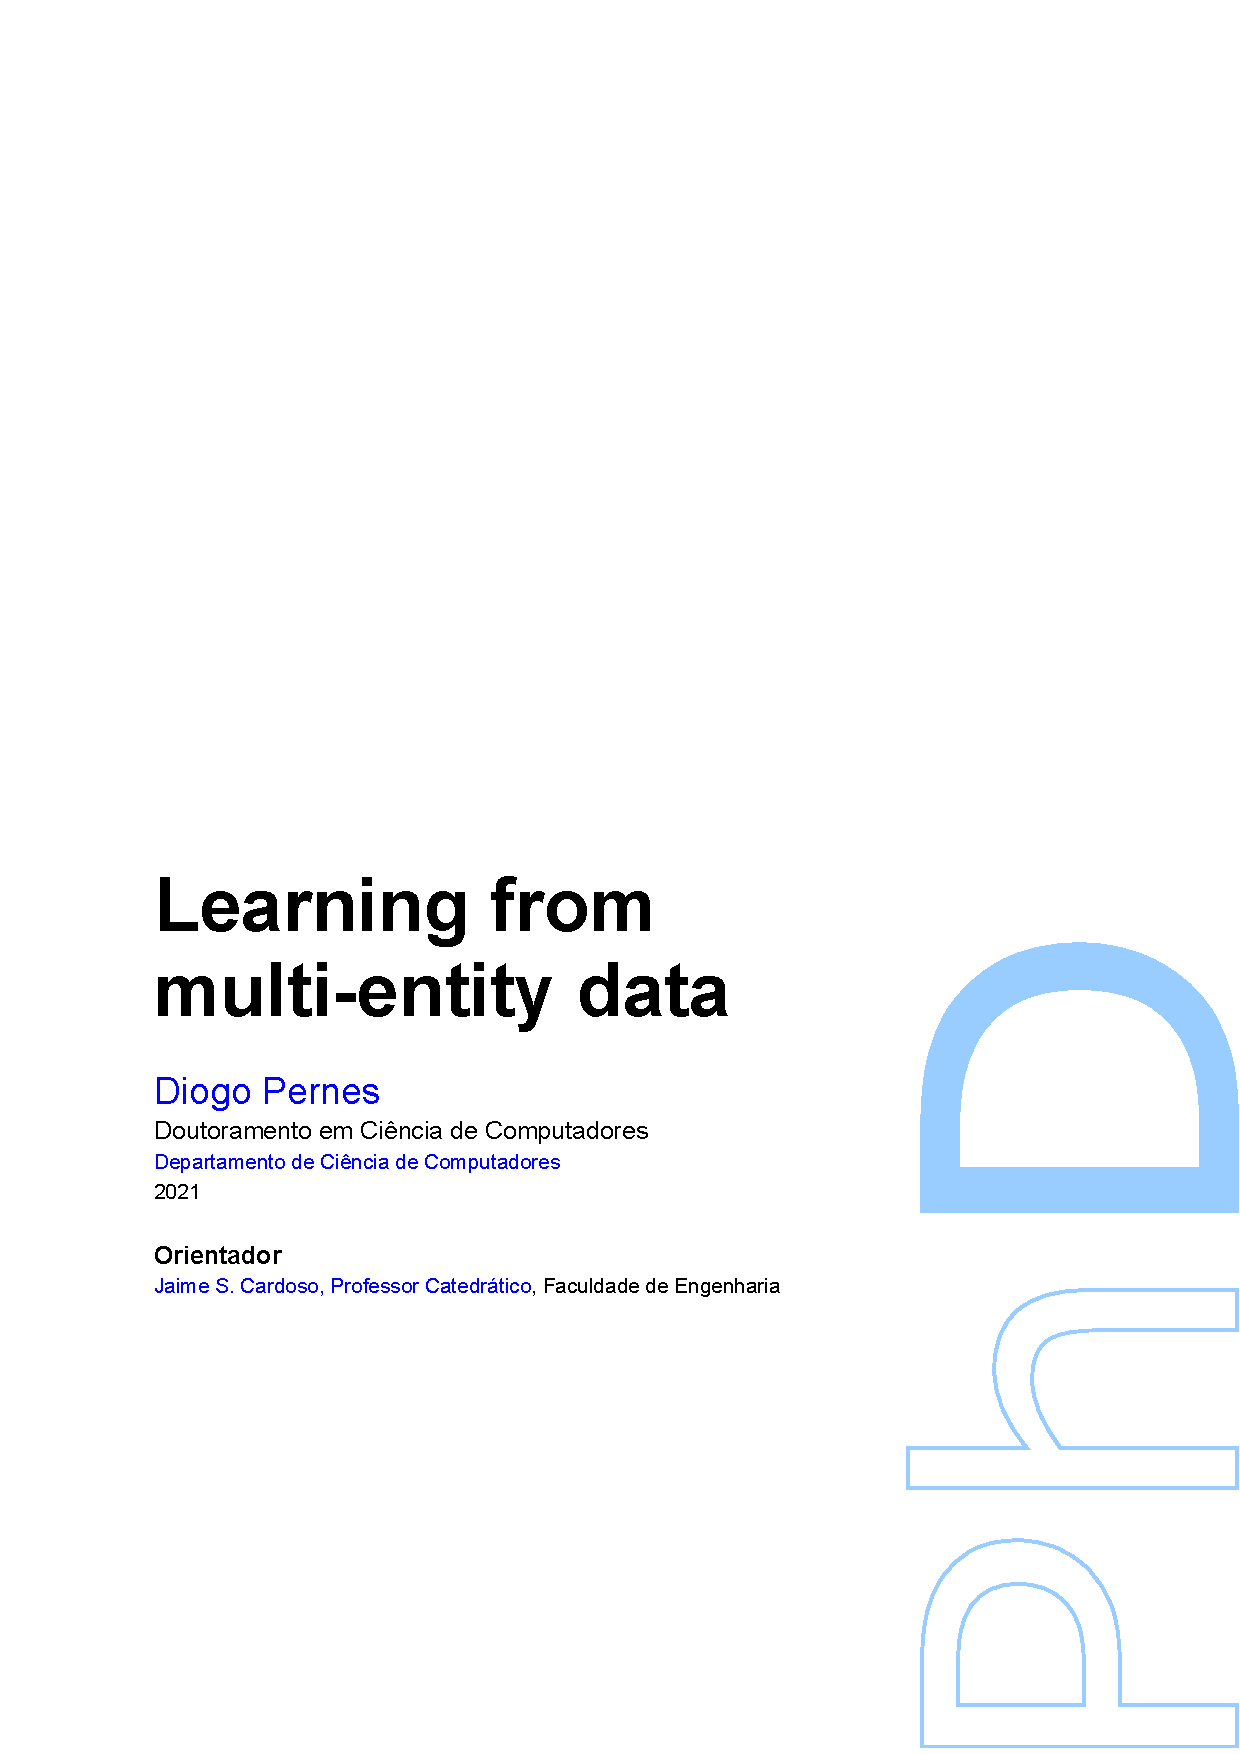
\includepdf[pages={1},pagecommand={},scale=1]{Front/main}
%\cleardoublepage
%\includepdf[pages={2},pagecommand={},scale=1]{Front/main}
%\cleardoublepage
%\pagestyle{fancy}

% Use roman page numbering style (i, ii, iii, iv...) for the pre-content pages
\frontmatter

% Title page
\maketitle

% Edit this file!

%-------------------------------------------------------------------------
%	QUOTATION PAGE
%-------------------------------------------------------------------------
\quotepage{Alan Turing}
{
	The original question, ‘Can machines think?’ I believe to be too meaningless to deserve discussion.
}

%-------------------------------------------------------------------------
%	ACKNOWLEDGEMENTS PAGE
%-------------------------------------------------------------------------
\begin{acknowledgements}
\begin{otherlanguage}{portuguese}
Esta tese foi financiada pela Fundação para a Ciência e a Tecnologia (FCT), no âmbito da bolsa de doutoramento SFRH/BD/129600/2017.

Gostaria de expressar o meu agradecimento ao INESC TEC, instituição de acolhimento do meu doutoramento, à Faculdade de Ciências da Universidade do Porto, pela oferta do programa doutoral, e à Faculdade de Engenharia da Universidade do Porto, por me ter proporcionado a honra e o enorme prazer de lecionar duas unidades curriculares de um dos seus planos de estudos.

A nível pessoal, manifesto a minha profunda gratidão ao meu orientador, Prof.\ Jaime S.\ Cardoso, inexcedível no apoio, disponibilidade, supervisão, paciência e compreensão em momentos difíceis, qualidades a que alia excelência científica inquestionável e amplamente reconhecida. Não posso também esquecer os meus professores Paula Malonek e Pedro Guedes de Oliveira, que muito me ajudaram e inspiraram no meu percurso académico anterior e me apoiaram e aconselharam na fase complicada que antecedeu o meu doutoramento.

Todos os atuais e anteriores membros do VCMI merecem a minha maior consideração e, em muitos casos, inestimável amizade. Trabalhar ao vosso lado e conviver convosco fez de mim uma pessoa melhor, tanto no plano profissional como pessoal. Um agradecimento especial aos coautores das minhas publicações, cujo contributo para esta tese foi absolutamente fundamental. Entre estes, tenho de destacar o Pedro Ferreira, não só pelo extenso trabalho que desenvolvemos em conjunto, mas também e sobretudo por ser um amigo insubstituível em todos os momentos.

Agradeço a todos os meus estudantes na FEUP, em particular àqueles que hoje tenho como amigos. Todas as horas que passámos, em aula e fora dela, ensinaram-me muito mais do que aquilo que vos lecionei. Espero que continuem a contar comigo e poder continuar a contar convosco.

Aos meus amigos de sempre e que nunca me falham, estando perto ou longe.

À Rita, por estar sempre comigo e me fazer desejar que assim seja para sempre. À minha família, o meu grande suporte. À minha mãe, pelo seu amor infinito e incondicional.

\vspace{11pt}

Ao meu pai e avós, com saudade imensa.

\end{otherlanguage}
\end{acknowledgements}

\addvspacetoc{0.3cm} % Add a gap in the Contents, for aesthetics


%-------------------------------------------------------------------------
%	ABSTRACT PAGE (PORTUGUESE)
%-------------------------------------------------------------------------
\begin{abstract}[
	thesistitle={Aprendizagem a partir de dados multi-entidade},
	title={Resumo},
	degree={Doutoramento em Ciência de Computadores},
	nameconnector={por}]
\begin{otherlanguage}{portuguese}

A maioria dos algoritmos de aprendizagem automática, em particular os concebidos para classificação supervisionada, assume que os dados nos quais irão ser treinados resultam de um processo de amostragem independente e identicamente distribuída. Este pressuposto ignora o facto de que, em muitos casos, o conjunto de treino disponível consiste numa coleção de subconjuntos, cada um deles proveniente da sua própria distribuição. O mesmo se aplica aos dados utilizados para teste e inferência, cuja distribuição associada difere frequentemente da observada durante o treino do modelo.

Nesta tese, abordamos, sob várias perspetivas, o problema de aprendizagem a partir de múltiplas distribuições. Em primeiro lugar, consideramos a situação em que várias fontes de dados coabitam no mesmo meio e originam sequências de dados. Neste contexto, demonstramos que é possível tirar partido das correlações existentes entre as várias fontes, obtendo-se um modelo generativo para estes dados cujo desempenho é superior ao resultante da aprendizagem a partir de cada uma das fontes separadamente.

Posteriormente, dedicamo-nos ao problema da generalização fora da distribuição de treino, isto é, ao desenvolvimento de modelos robustos quando testados em distribuições substancialmente diferentes da observada durante o treino. Inicialmente, consideramos o problema da adaptação de domínio a partir de múltiplas distribuições-fonte. Neste cenário, assume-se que, na fase de treino, estão disponíveis dados anotados provenientes de múltiplas distribuições-fonte e que se pretende obter um modelo de classificação com bom desempenho numa distribuição-alvo, fixa à partida, mas diferente de todas as distribuições-fonte e para a qual apenas estão disponíveis dados não anotados. No âmbito deste tema, investigamos diversas arquiteturas de redes neuronais para contagem de objetos em vídeos provenientes de múltiplas câmaras e propomos um novo algoritmo de adaptação de domínio para dados não sequenciais cujo desempenho supera o do estado da arte.

Finalmente, focamo-nos na generalização de domínio. Este problema difere da adapta-\allowbreak ção de domínio no sentido em que, desta vez, o domínio-alvo não é definido \emph{a priori}, pelo que, na fase de treino, não estão disponíveis quaisquer dados provenientes da distribuição-\allowbreak-alvo. O reconhecimento de língua gestual é a principal aplicação que utilizamos para motivar o problema e os algoritmos desenvolvidos, visto que um sistema de reconhecimento gestual realmente útil deve apresentar um bom desempenho independentemente do gestuante que o utiliza. Para este efeito, propomos dois algoritmos que permitem a obtenção de um classificador de gestos robusto a novos gestuantes. O primeiro destes consiste numa melhoria de um método pré-existente, baseado em redes neuronais adversárias. O segundo, que é também o que apresenta o melhor desempenho, utiliza um codificador automático variacional, que permite a aprendizagem de representações latentes independentes do gestuante e altamente discriminativas para a tarefa de classificação pretendida.

Esta tese é, assim, um trabalho abrangente na área de aprendizagem multi-entidade e multi-domínio. Como explicado anteriormente, tratamos vários problemas que se adequam a diferentes aplicações do mundo real, que frequentemente utilizamos para motivar e validar os algoritmos propostos. As contribuições aqui apresentadas resultaram em diversas publicações em revistas e conferências internacionais, que listamos no decorrer deste documento.


\end{otherlanguage}
\end{abstract}

%-------------------------------------------------------------------------
%	ABSTRACT PAGE
%-------------------------------------------------------------------------
\begin{abstract}

    Most machine learning algorithms, and particularly those conceived for supervised classification, assume that the data on which they are trained are independent and identically distributed (i.i.d.). This assumption ignores the fact that, in many circumstances, the available training data is a collection of sub-datasets, each one being originated at a distinct data source and hence being sampled from its own distribution. Furthermore, the data observed at test time often suffer from the same distribution shift problem, again violating the i.i.d.\ assumption.

    In this thesis, we address the problem of learning from multiple data distributions under various settings. First, we consider the case where multiple data sources are spread over a given medium and produce sequential data streams. Although the data distributions for each of the sources are different, we show that inter-source correlations can be exploited to learn a better-performing model for the generative distribution of each source.

    Afterward, we focus on out-of-distribution generalization, i.e.\ to the setting in which the test distribution is unknown or only partially known at training time. Initially, we consider the problem of multi-source domain adaptation. Here, annotated data from multiple data sources are combined to learn a classification model for a fixed target distribution, for which no labeled data is available at training time. We research several possible deep neural network architectures for object counting in videos from multiple cameras and propose a novel algorithm for multi-source domain adaptation for non-sequential data that achieves state-of-the-art results.

    Finally, we address domain generalization. This problem differs from domain adaptation in that the target domain is unknown, and therefore no data from this distribution is available at training time, neither labeled nor unlabeled. Sign language recognition is the main application considered here since a truly useful automatic sign language recognition system should be able to perform accurately regardless of the signer that is using it. We propose two algorithms to learn a signer-independent sign classifier. The first is an improvement over an existing method based on adversarial neural networks and the second and best-performing uses a variational autoencoder to learn highly discriminative signer-invariant representations.

    This thesis is then a broad-scope work focused on multi-entity and multi-domain learning. As explained before, we address multiple problem formulations that fit different practical applications, which are often used to motivate and validate the proposed algorithms. The contributions presented in this thesis resulted in publications in international journals and conferences, listed later in this document.

\end{abstract}

%-------------------------------------------------------------------------
%	LIST OF CONTENTS/FIGURES/TABLES
%-------------------------------------------------------------------------

\addvspacetoc{0.3cm}
\setcounter{tocdepth}{3}
\tableofcontents % Write out the Table of Contents

\listoffigures % Write out the List of Figures

%\listoftables % Write out the List of Tables

%\addvspacetoc{0.3cm}

%-------------------------------------------------------------------------
%	PHYSICAL CONSTANTS/OTHER DEFINITIONS
%-------------------------------------------------------------------------

%\begin{listofcontants}
%	\const{My little ponny test of magical rainbow}{$mn/mp$}
%    {$2.997\ 924\ 58\times10^{8}\ \mbox{ms}^{-\mbox{s}}$}
%   \const{Vaccuum permeability test of magical rainbow for a specific case of
%   condensed matter physics}
%   {$\epsilon_0$}{$2.997\ 924\ 58\times10^{8}\ \mbox{ms}^{-\mbox{s}}$}
%	\const{Speed of Light test of magical rainbow}{$c$}
%    {$2.997\ 924\ 58\times10^{8}\ \mbox{ms}^{-\mbox{s}}$}
%\end{listofcontants}


%-------------------------------------------------------------------------
%	SYMBOLS
%-------------------------------------------------------------------------

%\begin{listofsymbols}
%	\symb{$F_{\mu\nu}$}{Maxwell tensor}{F}
%	\symb{$a$}{distance}{m}
%	\\
%	\symb{$\omega$}{angular frequency}{rads$^{-1}$}
%\end{listofsymbols}


%-------------------------------------------------------------------------
%	NOTATION
%-------------------------------------------------------------------------

\newcommand\notationname{Notation and Conventions}
\addtotoc{\notationname}
\fancyhead[LO]{\textsc{\notationname}}

\input{Notation}



%-------------------------------------------------------------------------
%	ABBREVIATIONS
%-------------------------------------------------------------------------

\begin{glossary}
    \abbrev{AP}{access point}
    \abbrev{CNN}{convolutional neural network}
    \abbrev{CPD}{conditional probability distribution}
    \abbrev{CVAE}{conditional variational autoencoder}
    \abbrev{DA}{domain adaptation}
    \abbrev{DeSIRe}{deep signer invariant representations (model name)}
    \abbrev{DG}{domain generalization}
    \abbrev{DL}{deep learning}
    \abbrev{ELBO}{evidence lower bound}
    \abbrev{EM}{expectation-maximization}
    \abbrev{HMM}{hidden Markov model}
    \abbrev{LSTM}{long short-term memory}
    \abbrev{KL}{Kullback-Leibler}
    \abbrev{MAE}{mean absolute error}
    \abbrev{MAP}{maximum a posteriori}
    \abbrev{MDAN}{multi-source domain adversarial
networks}
    \abbrev{ME}{movement of epenthesis}
    \abbrev{MHMM}{mixture of hidden Markov models}
    \abbrev{MKLM}{Microsoft Kinect and Leap Motion (dataset)}
    \abbrev{MLLR}{maximum likelihood linear regression}
    \abbrev{MLP}{multi-layer perceptron}
    \abbrev{MODA}{multi-source mildly optimistic domain adaptation (model name)}
    \abbrev{MODA-FM}{MODA with FixMatch regularization (model name)}
    \abbrev{OOD}{out-of-distribution}
    \abbrev{PAD}{presentation attack detection}
    \abbrev{PAI}{presentation attack instrument}
    \abbrev{PAIS}{presentation attack instrument species}
    \abbrev{ReLU}{rectifier linear unit}
    \abbrev{RNN}{recurrent neural network}
    \abbrev{SOHMMM}{self-organizing hidden Markov model map}
    \abbrev{SOM}{self-organizing map}
    \abbrev{SpaMHMM}{sparse mixture of hidden Markov models}
    \abbrev{SLR}{sign language recognition}
    \abbrev{SSL}{self-supervised learning}
    \abbrev{STA}{wireless station}
    \abbrev{SVM}{support vector machine}
    \abbrev{t-SNE}{t-distributed stochastic neighbor embeddings}
    \abbrev{UBM}{universal background model}
    \abbrev{UDA}{unsupervised domain adaptation}
    \abbrev{VAE}{variational autoencoder}
    \abbrev{VSIA}{Visible Spectrum Iris Artefact (dataset)}
    \abbrev{wLBP}{weighted local binary pattern}
\end{glossary}


%-------------------------------------------------------------------------
%	DEDICATORY
%-------------------------------------------------------------------------

%\begin{dedicatory}
%	This thesis is dedicated to my family, for their love and support.
%\end{dedicatory}



%-------------------------------------------------------------------------
%	THESIS CONTENT - CHAPTERS
%-------------------------------------------------------------------------

\addvspacetoc{0.3cm}

% Begin numeric (1,2,3...) page numbering
\mainmatter

\pagestyle{fancy}
\renewcommand{\chaptermark}[1]{\markboth{\thechapter. \textsc{#1}}{}}
\fancyhead[LO]{\leftmark}

%%% -----------  ADD CHAPTERS HERE ------------------ %%%

% Chapter Template

% Main chapter title
%\chapter[toc version]{doc version}
\chapter{Background}

% Short version of the title for the header
%\chaptermark{version for header}

% Chapter Label
% For referencing this chapter elsewhere, use \ref{ChapterTemplate}
\label{chp:background}

% Write text in here
% Use \subsection and \subsubsection to organize text

\section{Introduction}
\label{sec:background_intro}
We will use deep neural networks and probabilistic models extensively throughout this thesis. Although the basic concepts of the former should be fairly familiar to most readers, the latter might be less widely known. Moreover, some of the tools and algorithms that we are going to use are not so trivial and therefore they should better be introduced first, for the sake of completeness and readability.

This chapter will then focus on providing a brief yet rigorous background on the aforementioned subject. We shall start by clarifying some notation and conventions we shall adopt (\Secref{sec:definitions}). Then we proceed with a short introduction to Bayesian networks, motivated by the factorization properties of joint probability functions (\Secref{}). Expectation-Maximization (EM) is presented as an efficient algorithm to learn probabilistic models with unobserved variables (\Secref{}). We then review the hidden Markov model (HMM), which will play a central role in Chapter \ref{chp:networked_data_streams}, and present the instantiation of the EM algorithm for this particular model (\Secref{}). The chapter is concluded with a brief introduction to variational inference (\Secref{}). Under this setting, the variational autoencoder will deserve special attention (\Secref{}), as it will be one of the models employed in Chapter \ref{chp:domain_generalization}.

\section{Useful definitions and conventions}
\label{sec:definitions}
In this section, we introduce some further notations and definitions that will be used throughout this document.

It is important to remark that the same notation is used to denote discrete and continuous random variables as well as to denote probability mass functions and probability density functions. Specifically, given a random variable $\rx$ defined in $\gX$, $p(\rx)$ denotes the probability mass of $\rx$, if $\gX$ is discrete, or the probability density of $\rx$, otherwise. In either case, the \emph{support} of $p(\rx)$ is defined as $\mathrm{Supp}(p(\rx)) \triangleq \lbrace x \in \gX: p(\rx=x) > 0 \rbrace$. Moreover, when we want to denote the probability (density) of some arbitrary but fixed value $x \in \gX$, we often use $p(x)$ as a short for $p(\rx=x)$.

The joint probability function of $\rx$ and $\ry$ is denoted by $p(\rx,\ry)$ and the corresponding conditionals of $\ry$ given $\rx$ and $\rx$ given $\ry$ are denoted by the usual $p(\ry \mid \rx)$ and $p(\rx \mid \ry)$, respectively. Again, $\rx$ and $\ry$ can be both discrete, both continuous, or one continuous and the other discrete. For three or more random variables the notation generalizes naturally.

The marginalization of $p(\rx,\ry)$ with respect to a discrete $\ry$ is written as:
\begin{equation}
  \sum_{\ry} p(\rx,\ry) \triangleq \sum_{y \in \gY} p(\rx,y) = p(\rx),
\end{equation}
and the marginalization of $p(\rx,\ry)$ with respect to a continuous $\rx$ is written as:
\begin{equation}
    \int p(\rx,\ry) \d \rx \triangleq \int_{\gX} p(x,\ry) \d x = p(\ry).
\end{equation}
Note that for brevity we omit the domain of the summation or integration, as this is defined implicitly by the set where the random variable is defined. The integral notation is also used for the marginalization with respect to random variables whose type is unspecified. Similarly, if $f(\rx)$ is a function of a random variable $\rx$,
\begin{equation}
    \sum_\rx f(\rx) \triangleq \sum_{x \in \gX} f(x) \quad \text{or} \quad \int f(\rx) \d \rx \triangleq \int_\gX f(x) \d x,
\end{equation}
depending on whether $\rx$ is discrete or continuous, respectively. Hence, we can write the \emph{expectation} of $f(\rx)$ with respect to $p(\rx)$ as:
\begin{equation}
    \E_{\rx \sim p(\rx)} \left[f(\rx)\right] \triangleq \sum_\rx f(\rx) p(\rx) \quad \text{or} \quad \E_{\rx \sim p(\rx)} \left[f(\rx)\right] \triangleq \int f(\rx) p(\rx) \d \rx,
\end{equation}
for a discrete or continuous $\rx$, respectively.

\section{Bayesian networks}
\label{sec:bayesian_networks}

Given $n$ random variables $\rx_1, \rx_2, \dots, \rx_n$, the \emph{chain rule of probability} allows the factorization of their joint distribution as:\footnote{The expression on the right-hand side of \eqref{eq:chain_rule} is not well defined outside the support of $p(\rx_1), p(\rx_1, \rx_2), \dots, p(\rx_1, \rx_2, \dots, \rx_{n-1})$. For those values, one has $p(\rx_1, \rx_2, \dots, \rx_n)=0$.}
\begin{equation}
    \label{eq:chain_rule}
    p(\rx_1,\rx_2,\dots,\rx_n) = p(\rx_1) \prod_{i=1}^n p(\rx_i \mid \rx_{i-1}, \rx_{i-2}, \dots, \rx_1).
\end{equation}
Starting from this product, we may build a directed graph with $n$ vertices, one for each random variable, where there exists an edge $i \rightarrow j$ if and only there is a factor where $\rx_i$ is conditioned on $\rx_j$. Such a graph is known as a \emph{Bayesian network}. From its definition, it is clear that the factorization in \eqref{eq:chain_rule} corresponds to the graph in \Figref{fig:complete_bayesian_net}. Clearly, a Bayesian network defines a bijection between random variables and graph nodes, so with a slight abuse of terminology we represent and refer to nodes by the random variable they are associated with, rather than by their index.

\begin{figure}
    \centering
    \begin{tikzpicture}[auto, node distance=3cm, every loop/.style={},thick,
            main node/.style={circle,draw,font=\sffamily\Large\bfseries},
            hidden node/.style={circle,draw,fill=lightgray,font=\sffamily\Large\bfseries},
            box node/.style={rectangle,dashed,draw,anchor=center},
            empty node/.style={rectangle,fill=white,anchor=center},]


            \node[main node,minimum size=1.5cm] (x1) {$\rx_1$};
            \node[main node,minimum size=1.5cm] (x2) [right of=x1] {$\rx_2$};
            \node[main node,minimum size=1.5cm] (x3) [right of=x2] {$\rx_3$};
            \node[empty node] (dots) [right of=x3] {$\dots$};
            \node[main node,minimum size=1.5cm] (xn) [right of=dots] {$\rx_n$};


            \draw[->]
            (x1) edge (x2)
            (x2) edge (x3)
            (x3) edge (dots)
            (dots) edge (xn)
            (x1) edge[bend right] (x3)
            (x1) edge[bend right] (dots)
            (x1) edge[bend right] (xn)
            (x2) edge[bend right] (dots)
            (x2) edge[bend right] (xn)
            (x3) edge[bend right] (xn);

    \end{tikzpicture}
    \caption{Bayesian network corresponding to \eqref{eq:chain_rule}.}
    \label{fig:complete_bayesian_net}
\end{figure}
Since the factorization in \eqref{eq:chain_rule} is general (i.e.\ it does not assume any conditional independence between random variables), the Bayesian network in \Figref{fig:complete_bayesian_net} is said to be \emph{complete}.

% Chapter Template

% Main chapter title
%\chapter[toc version]{doc version}
\chapter{Networked data streams}

% Short version of the title for the header
%\chaptermark{version for header}

% Chapter Label
% For referencing this chapter elsewhere, use \ref{ChapterTemplate}
\label{chp:networked_data_streams}

% Write text in here
% Use \subsection and \subsubsection to organize text


\begin{tcolorbox}
	\small{
		The content presented in this Chapter was partially published in or adapted from \cite{SpaMHMM, SOHMMM}.
	}
\end{tcolorbox}

\section{Motivation}
\label{sec:chp1_motivation}
A broad range of real-life settings can be well modeled by an arbitrary number of network connected entities that share and interact in the same medium and generate data streams in real-time. The streams produced by each of these entities form a set of time series with both intra- and inter-correlations between them. In neuroimaging studies, the brain can be regarded as a network: a connected system where nodes, or units, represent different specialized regions and links, or connections, represent communication pathways. From a functional perspective, communication is coded by temporal dependence between the activities of different brain areas (\citet{DeVicoFallani20130521}). Also team sports intrinsically involve fast, complex and interdependent events among a set of entities (the players), which interact as a team (\citet{Tora2017, Theagarajan2018}). The emergence of vehicular networks is also generating an ever-increasing amount of network data (\citet{Cheng2018}), where interactions between neighboring vehicles may be exploited to build more accurate and reliable learning algorithms. Thus, in all these scenarios the behavior of each individual entity is better understood if its context information (i.e.\ the behavior of the neighboring instances) is leveraged. However, the extraction of knowledge from these streams to support the decision-making process is still challenging. Moreover, conventional algorithms that assume ability to store and centralize all the data in memory at the same time are impractical for many applications (\citet{Gama2007}).

Modeling the generative process of distributed stream data is an unsupervised learning problem and, hence, a model can be learned directly from the large amounts of data that might be continuously produced or gathered at each network connected entity, without the requirement of any special human supervision or annotation. Moreover, generative models are powerful tools for a wide variety of problems that arise naturally in networked data streams, like anomaly and novelty detection, sequence forecasting, clustering, and network simulation. Hence, generative models for stream data have been developed and applied in several previous works (e.g.\ \citet{Laxman2008, Hayat2010, Hofmann2011}). However, to the best of our knowledge, this problem is seldom explored in the  distributed setting.

Given the distributed nature of network data and the high information rate that those streams could have, we argue that such generative model and/or the associated learning algorithm should ideally satisfy the following properties:
\begin{enumerate}
	\item Learning and inferring distributedly, i.e.\ each entity should be able to update its own model and perform inference on it without observing the streams or the models associated with the remaining entities.
	\item Learning online, i.e.\ in real-time and without the requirement of storing the whole dataset in memory.
	\item Leveraging contextual information by incorporating prior knowledge about similarities and dissimilarities among sets of entities.
	\item Universality, i.e.\ the model should be applicable to a wide variety of distributed stream data, of diverse nature.
\end{enumerate}
In this chapter, we present two solutions for this problem, each with its own advantages and drawbacks. Both are inspired on the concept of sparse representations, which expresses a signal/model $f$, defined over some independent variable $x$, as a linear combination of a few atoms from a prespecified and overcomplete dictionary of size $M$:
\begin{equation}
\label{sparse_coding}
f(x)=\sum_{m=1}^M s_m \phi_m(x),
\end{equation}
where $\phi_m(x)$ are the atoms and only a few of the scalars $s_m$ are non-zero, providing a sparse representation of $f(x)$.  Distributed sparse representation (\citet{Baron}) is an extension of the standard version that considers networks with $K$ nodes. At each node, the signal sensed at the same node has its sparsity property because of its intracorrelation, while, for networks with multiple nodes, signals received at different nodes also exhibit strong intercorrelation.
The intra- and inter-correlations lead to a joint sparse model. An interesting scenario in distributed sparse representation, which we exploit here, is when all signals/models share the common support but with different non-zero coefficients.

Our contributions in this chapter are summarized as follows: i) we extend an existing model based on a combination of self-organizing maps (SOM) and HMMs and evaluate it in the context of anomaly detection in Wi-Fi networks; ii) we present a novel algorithm that learns an entity-dependent model based on a mixture of shared HMMs; iii) we discuss how the two models intersect each other and, importantly, how the latter can be viewed as a particular case of a general family of generative models for distributed data.

\section{Hidden Markov Models on a Self-Organizing Map for Anomaly Detection in 802.11 Wireless Networks}
\label{sec:sohmmm}

\subsection{Related work}
A number of studies in the literature have integrated the SOM and HMM in different manners. In \citet{Ref15}, the spherical self-organizing map (S-SOM) is proposed, which uses HMM models as neurons (S-HMM-SOM) to classify the time-series data. Despite our work, the HMM models in \citet{Ref15} are discrete and the author applied the  Baum-Welch algorithm for updating the model parameters. In \citet{Ref16}, the authors extended the self-organizing mixture models for multivariate time-series, assuming that the time-series are generated by HMMs. This model, which is called a self-organizing hidden Markov model (SOHMM), uses constrained expectation maximization (EM) for HMM parameter estimation. The self-organization in this work is used for meteorological-state visualization. 

In another direction of work in \citet{Ref21}, a SOMM-based architecture is presented for hand-gesture recognition. The approach involves a combination of SOMs and Markov models for gesture-trajectory classification. In this work, the neurons on the SOM map correspond to the states of the Markov models. In \citet{Ref24}, the combination of the SOM and HMM (SOS-HMM: self-organizing structure of HMM) automatically extracts the structure of an HMM without any prior knowledge of the application domain. In this model, the macro-HMM is represented as a graph of macro-states, where each state represents a micro-HMM. In summary, each neuron in the SOM-HMM collaborative architecture is either an HMM by itself or a hidden state. In our work, each particular neuron on the SOM lattice is associated with an HMM. 

In \citet{Ref39}, a probabilistic self-organizing map called PrSOMS is presented for the clustering and visualization of dependent and non-identically distributed data. In this model, the SOM learning paradigm to produce topology-preserving maps is combined with the probabilistic-learning scheme of the HMM. The SOM is considered to be a grid, forming a discrete topology in which each cell represents a state; the parameters of the model are estimated by maximizing the likelihood of the sequential data set. In another direction of work in \citet{Ref41}, the effects of meteorological factors on the occurrence of strokes are investigated. The authors used the SOM to obtain weather patterns that would serve as states of the HMMs. They showed that HMMs with states given by the SOM are useful for describing a background process of stroke incidence. This approach considers the SOM as a front-end processor.

In \citet{Ref1,Ref37,Ref38}, the fusion and synergy of SOMs and HMMs are employed in biological-molecule studies to meet the increasing requirements imposed by the properties of deoxyribonucleic acid (DNA), ribonucleic acid (RNA), and protein chain molecules. The authors proposed a stochastic unsupervised-learning algorithm based on the integration of the SOM and HMM principles, called SOHMMM. The SOHMMM's characteristics and capabilities are demonstrated through two series of experiments, based on artificial sequence data and splice-junction gene sequences. However, in these papers, only the discrete-observation setting is addressed. Here, we extend the algorithm for multivariate Gaussian in order to fit the requirements of our anomaly-detection project.

Incremental learning of HMM parameters is the core function of the SOHMMM algorithm, which is based on a stochastic gradient-descent technique. The incremental learning of new data sequences allows HMM parameters to adapt as new data become available, without having to retrain from the start on all the accumulated training data. Various techniques in the literature address this topic. These techniques are classified according to the objective function, optimization technique, and target application, involving the block-wise and symbol-wise learning of parameters. The authors in \citet{Ref25} presented a comprehensive survey of techniques that are suitable for the incremental learning of HMM parameters, among which, the stochastic gradient-descent technique of the SOHMMM is referred to as one of the numerical-optimization methods.

Additionally, few efforts exist in the literature that exploit the SOM and HMM for anomaly-detection purposes \citet{Ref22,Ref23}. In \citet{Ref22}, the authors presented an intrusion-detection system in which the SOM determines the optimal measures of audit data and reduces them to an appropriate size for efficient modeling by the HMM. Similar to our previous work \citet{Ref5}, two types of HMM are utilized: a single model for all the users and individual models for each user. In another relevant work in \citet{Ref23}, the HMM and the SOM are investigated separately as intrusion-detection techniques. The testing results show that the HMM method using the events' transition property outperformed the SOM using the events' frequency property. Regarding the same subject of intrusion detection, the SOM and HMM have a collaborating connection in \citet{Ref22} and competitive roles in \citet{Ref23}.

In this work, we intend to benefit from the collaboration of these two techniques (SOM and HMM), as proposed by \citet{Ref38}, to extend previous anomaly-detection frameworks applying only HMM (\citet{Ref7,Ref6,Ref5}).

\section{SpaMHMM: Sparse Mixture of Hidden Markov Models}
\label{sec:spamhmm}

\subsection{Overview}

Inspired by the formulation of \eqref{sparse_coding}, we propose to model the generative distribution of the data coming from each of the $K$ nodes of a network as a sparse mixture obtained from a dictionary of generative distributions. Specifically, we shall model the distribution for each node as a sparse mixture over a `large' shared dictionary of HMMs, where each HMM corresponds to an individual atom from the dictionary.
The field knowledge about the similarities between nodes is summarized in an affinity matrix. The objective function of the learning process promotes reusing HMM atoms between similar nodes.
We now formalize these ideas.

\subsection{Model formulation}
\subsubsection{Definition}
\label{sec:definition}
Assume we have a set of nodes $\sY=\{1, ..., K\}$ connected by an undirected weighted graph $\gG$, expressed by a symmetric matrix $\mG \in \R^{K \times K}$. These nodes thus form a network, in which the weights are assumed to represent degrees of affinity between each pair of nodes (i.e.\ the greater the edge weight, the more the respective nodes \textit{like} to agree). The nodes $\ry$ in the graph produce $D$-dimensional sequences $\rmX = \left(\rvx^{(1)}, ...,\rvx^{(T)} \right)$, $\rvx^{(t)} \in \R^D$, whose conditional distribution we shall model using a mixture of HMMs:
\begin{equation}
\label{hmm_mix}
p(\rmX \mid \ry) = \sum_{\rz} p(\rz\mid\ry) p(\rmX \mid \rz),
\end{equation}
where $\rz \in \{1, ..., M\}$ is a latent random variable, being $M$ the size of the mixture. This is a particular realization of \eqref{sparse_coding} where $f$ is the probability density function $p(\rmX \mid \ry)$ and the coefficients $s_m$ correspond to the probabilities $p(\rz = m \mid \ry)$. Here, $p(\rmX \mid \rz)$ is the marginal distribution of observations of a standard first-order homogeneous HMM:
\begin{equation}
\label{hmm}
p(\rmX \mid \rz) = \sum_{\rvh} p(\rh^{(0)}\mid\rz) \prod_t p(\rh^{(t)}\mid\rh^{(t-1)},\rz) p(\rvx^{(t)}\mid\rh^{(t)},\rz),
\end{equation}
where $\rvh = \left(\rh^{(0)}, ...,\rh^{(T)} \right)$, $\rh^{(t)} \in \{1, ..., S\}$, is the sequence of hidden states of the HMM, being $S$ the number of hidden states. Note that the factorization in \eqref{hmm_mix} imposes conditional independence between the sequence $\rmX$ and the node $\ry$, given the latent variable $\rz$. This is a key assumption of this model, since this way the distributions for the observations in the nodes in $\sY$ share the same dictionary of HMMs, promoting parameter sharing among the $K$ mixtures.

\subsubsection{Inference}
\label{sec:inference}
Given an observed sequence $\mX$ and its corresponding node $y \in \sY$, the inference problem here consists in finding the likelihood $p(\rmX=\mX \mid \ry=y)$ (from now on, abbreviated as $p(\mX \mid y)$) as defined by  \twoeqrefs{hmm_mix}{hmm}. The marginals $p(\mX\mid\rz)$ of each HMM in the mixture may be computed efficiently, in $O(S^2T)$ time, using the Forward algorithm~\citet{Rabiner1986}. Then, $p(\mX \mid y)$ is obtained by applying \eqref{hmm_mix}, so inference in the overall model is done in at most $O(MS^2T)$ time. As we shall see, however, the mixtures we get after learning will often be sparse (see \Secref{sec:learning}), leading to an even smaller time complexity.

\subsubsection{Learning}
\label{sec:learning}
Given an i.i.d. dataset consisting of $N$ tuples $(\mX_i, y_i)$ of sequences of observations $\mX_i = \left(\vx_i^{(1)}, ...,\vx_i^{(T_i)} \right)$ and their respective nodes $y_i \in \sY$, the model defined by \twoeqrefs{hmm_mix}{hmm} may be easily trained using the Expectation-Maximization (EM) algorithm \citet{Dempster1977}, (locally) maximizing the usual log-likelihood objective:
\begin{equation}
\label{log_likelihood}
J(\theta) = \sum_{i=1}^N \log p(\mX_i \mid y_i, \theta),
\end{equation}
where $\theta$ represents all model parameters, namely:
\begin{enumerate}
	\item the $M$-dimensional mixture coefficients, $\valpha_k \coloneqq \left(p(\rz=1\mid\ry=k), ..., p(\rz=M\mid\ry=k)\right)$, for $k = 1,...,K$;
	\item the $S$-dimensional initial state probabilities, $\vpi_m \coloneqq \left(p(\rh^{(0)}=1 \mid \rz=m),...,p(\rh^{(0)}=S \mid \rz=m)\right)$, for $m = 1,...,M$;
	\item the $S \times S$ state transition matrices, $\mA^m$, where $\emA^m_{s,u} \coloneqq p(\rh^{(t)}=u \mid \rh^{(t-1)}=s, \rz=m)$, for $s,u = 1,...,S$ and $m = 1,...,M$;
	\item the emission probability means, $\vmu_{m,s} \in \mathbb{R}^D$, for $m = 1,...,M$ and $s = 1,...,S$;
	\item the emission probability diagonal covariance matrices, $\mI \vsigma^2_{m,s}$, where $\vsigma^2_{m,s} \in \mathbb{R}^{D}_{+}$, for $m = 1,...,M$ and $s = 1,...,S$.
\end{enumerate}

Here, we are assuming that the emission probabilities $p(\rx^{(t)}\mid\rh^{(t)},\rz)$ are Gaussian with diagonal covariances. This introduces almost no loss of generality, since the extension of this work to discrete observations or other types of continuous emission distributions is straightforward.

The procedure to maximize objective~\plaineqref{log_likelihood} using EM is described in \Algref{alg:mhmm}. The update formulas follow from the standard EM procedure and can be obtained by viewing this model as a Bayesian network or by following the derivation detailed in \Secref{sec:proof_em_noreg}. However, the objective \plaineqref{log_likelihood} does not take advantage of the known structure of $\gG$. In order to exploit this information, we introduce a regularization term, maximizing the following objective instead:
\begin{align}
\label{objective}
J_r(\theta) &= \frac{1}{N}\sum_{i=1}^N \log p(\mX_i \mid y_i, \theta) \nonumber\\ 
&\mathbin{\hphantom{=}}{}+ \frac{\reg}{2} \sum_{\substack{j,k=1,\\k\neq j}}^{K} \emG_{j,k} \E_{\rz \sim p(\rz \mid \ry=j, \theta)} [ p(\rz \mid \ry=k, \theta) ] \nonumber\\
&= \frac{1}{N}\sum_{i=1}^N \log p(\mX_i \mid y_i, \theta) + \frac{\reg}{2} \sum_{\substack{j,k=1,\\k\neq j}}^{K} \emG_{j,k} \valpha_j^\top \valpha_k,
\end{align}
where $\reg \geq 0$ controls the relative weight of the two terms in the objective. Note that this regularization term favors nodes connected by edges with large positive weights to have similar mixture coefficients and thus share mixture components. On the other hand, nodes connected by edges with large negative weights will tend to have orthogonal mixture coefficients, being described by disjoint sets of components. These observations agree with our prior assumption that the edge weights express degrees of similarity between each pair of nodes. Proposition \ref{prop_expectations} formalizes these statements and enlightens interesting properties about the expectations $\E_{\rz \sim p(\rz \mid \ry=j, \theta)} [ p(\rz \mid \ry=k, \theta)]$.
\begin{proposition}
	\label{prop_expectations}
	For any integer $M>1$, let $\sP_M$ be the set of all probability distributions over the set $\{1,2\cdots,M\}$. We have:
	\begin{enumerate}
		\item $\min_{p,q \in \sP_M} \E_{\rz\sim p} [ q(\rz) ] = 0$; \label{prop_min}
		\item $\argmin_{p,q \in \sP_M} \E_{\rz\sim p} [ q(\rz) ] = \{p,q \in \sP_M \mid \forall \, m \in \{1,...,M\}: p(\rz = m)q(\rz = m)=0\}$; \label{prop_argmin}
		\item $\max_{p,q \in \sP_M} \E_{\rz\sim p} [ q(\rz) ] = 1$; \label{prop_max}
		\item $\argmax_{p,q \in \sP_M} \E_{\rz\sim p} [ q(\rz) ] = \{p,q \in \sP_M \mid \exists \, m \in \{1,...,M\} : \, p(\rz = m)=q(\rz = m)=1\}$ \label{prop_argmax}.
	\end{enumerate}
\end{proposition}
\begin{proof}
	By the definition of expectation,
	\begin{equation}
	\label{prop_expdef}
	\E_{\rz\sim p} [ q(\rz) ] = \sum_{m=1}^M p(\rz=m) q(\rz=m).
	\end{equation}
	Statements \ref{prop_min} and \ref{prop_argmin} follow immediately from the fact that every term in the right-hand side of \plaineqref{prop_expdef} is non-negative and $M>1$. For the remaining, we rewrite \plaineqref{prop_expdef} as the dot product of two $M$-dimensional vectors $\valpha_p$ and $\valpha_q$, representing the two distributions $p$ and $q$, respectively, and we use the following linear algebra inequalities to build an upper bound for this expectation:
	\begin{equation}
	\label{prop_ineq}
	\E_{\rz\sim p} [ q(\rz) ] = \valpha_p ^\top \valpha_q \leq || \valpha_p ||_2 || \valpha_q ||_2 \leq || \valpha_p ||_1 || \valpha_q ||_1 =1,
	\end{equation}
	where $||\bcdot||_1$ and $||\bcdot||_2$ are the $\normlone$ and $\normltwo$ norms, respectively. Clearly, the equality $\E_{\rz\sim p} [ q(\rz) ] = 1$ holds if $p$ and $q$ are chosen from the set defined in statement \ref{prop_argmax}, where the distributions $p$ and $q$ are the same and they are non-zero for a single assignment of $\rz$. This proves statement \ref{prop_max}. Now, to prove statement \ref{prop_argmax}, it suffices to show that there are no other maximizers. The first inequality in \plaineqref{prop_ineq} is transformed into an equality if and only if $\valpha_p = \valpha_q$, which means $p \equiv q$. The second inequality becomes an equality when the $\normlone$ and $\normltwo$ norms of the vectors coincide, which happens if and only if the vectors have only one non-zero component, concluding the proof.
\end{proof}
Specifically, given two distinct nodes $j, k \in \sY$ , if $\emG_{j,k} > 0$, the regularization term for these nodes is maximum (and equal to $\emG_{j,k}$) when the mixtures for these two nodes are the same and have one single active component (i.e.\ one mixture component whose coefficient is non-zero). On the contrary, if $\emG_{j,k} < 0$, the term is maximized (and equal to zero) when the mixtures for the two nodes do not share any active components. In both cases, though, we conclude from Proposition \ref{prop_expectations} that we are favoring sparse mixtures. We see sparsity as an important feature since it allows the size $M$ of the dictionary of models to be large and therefore expressive without compromising our rational that the observations in a given node are well modeled by a mixture of only a few HMMs. This way, some components will specialize on describing the behavior of some nodes, while others will specialize on different nodes. Moreover, sparse mixtures yield faster inference, more interpretable models and (possibly) less overfitting.
By setting $\reg=0$, we clearly get the initial objective \plaineqref{log_likelihood}, where inter-node correlations are modeled only via parameter sharing. As $\reg \to \infty$, two interesting scenarios may be anticipated. If $\emG_{j,k} > 0, \, \forall j,k \in \sY,$ all nodes will tend do share the same single mixture component, i.e.\ we would be learning one single HMM to describe the whole network. If $\emG_{j,k} < 0, \, \forall j,k \in \sY,$ and $M \geq K$, each node would tend to learn its own HMM model independently from all the others. Again, in both scenarios, the obtained mixtures are sparse.

The objective function~\plaineqref{objective} can still be maximized via EM (see details in \Secref{sec:proof_em_reg}). However, the introduction of the regularization term in the objective makes it impossible to find a closed form solution for the update formula of the mixture coefficients. Thus, in the M-step, we need to resort to gradient ascent to update these parameters. In order to ensure that the gradient ascent iterative steps lead to admissible solutions, we adopt the following reparameterization from \citet{Yang2018}:
\begin{equation}
\label{normalization}
\alpha_{k,m} = \frac{\sigma \left(\beta_{k,m} \right)^2}{\sum_{l=1}^M \sigma \left( \beta_{k,l} \right)^2}, 
\end{equation}
for $k = 1, ..., K$ and $m = 1, ..., M$, and where $\sigma(\bcdot)$ is the rectifier linear (ReLU) function. This reparameterization clearly resembles the softmax function, but, contrarily to that one, admits sparse outputs. The squared terms in \eqref{normalization} aim only to make the optimization more stable. The optimization steps for the objective \plaineqref{objective} using this reparameterization are described in \Algref{alg:spamhmm}.

\begin{algorithm}
	\caption{EM algorithm for the mixture without regularization (MHMM).}
	\label{alg:mhmm}
	\begin{algorithmic}
		\State Inputs: The training set, consisting of $N$ tuples $(\mX_i,y_i)$, a set of initial parameters $\theta^{(0)}$ and the number of training iterations $\mathcal{I}$.
		\For{$j = 1, ..., \mathcal{I}$}
		\State Sufficient statistics:
		\begin{enumerate}
			\item $n_k \coloneqq \sum_i \1_{y_i=k}$, where $\1_\mathrm{(\bcdot)}$ is the indicator function, for $k=1,...,K$.
			\item Obtain the mixture posteriors $\eta_{i,m} \coloneqq p(\rz=m|\mX_i, y_i,\theta^{(j-1)})$, for $i=1,...,N$ and $m=1,...,M$, by computing  $\tilde{\eta}_{i,m} \coloneqq p(\mX_i|\rz=m, \theta^{(j-1)})p(\rz=m|y_i, \theta^{(j-1)})$ and normalizing it.
			\item Obtain the state posteriors $\gamma_{i,m,s}(t) \coloneqq p(\rh^{(t)}=s | \rz=m, \mX_i, \theta^{(j-1)})$ and $\xi_{i,m,s,u}(t) \coloneqq p(\rh^{(t-1)}=s, \rh^{(t)}=u | \rz=m, \mX_i, \theta^{(j-1)})$, for $i=1,...,N$, $m=1,...,M$ and $s,u=1,...,S$, as done in the Baum-Welch algorithm \citet{Baum1972}.
		\end{enumerate}
		\State M-step:
		\begin{enumerate}
			\item $\evalpha_{k,m} = \frac{\sum_i \eta_{i,m} \1_{y_i=k}}{n_k}$, for $k=1,...,K$ and $m=1,...,M$, obtaining $\valpha_k$.
			\item $\evpi_{m,s} = \frac{\sum_i \eta_{i,m} \gamma_{i,m,s}(0)}{\sum_i \eta_{i,m}}$, for $m=1,...,M$ and $s=1,...,S$, obtaining $\vpi_{m}$. 
			\item $\emA^m_{s,u} = \frac{\sum_i \eta_{i,m} \sum_{t=1}^{T_i} \xi_{i,m,s,u}(t)}{\sum_i \eta_{i,m} \sum_{t=0}^{T_i-1} \gamma_{i,m,s}(t)}$, for $m=1,...,M$ and $s,u=1,...,S$, obtaining $\mA^m$.
			\item $\vmu_{m,s} = \frac{\sum_i \eta_{i,m} \sum_{t=1}^{T_i} \gamma_{i,m,s}(t) \vx_i^{(t)}} {\sum_i \eta_{i,m} \sum_{t=1}^{T_i} \gamma_{i,m,s}(t)}$, for $m=1,...,M$ and $s=1,...,S$.
			\item $\vsigma^2_{m,s} = \frac{\sum_i \eta_{i,m} \sum_{t=1}^{T_i} \gamma_{i,m,s}(t) \left(\vx_i^{(t)} - \boldsymbol{\mu}^m_s\right)^2} {\sum_i \eta_{i,m} \sum_{t=1}^{T_i} \gamma_{i,m,s}(t)}$, for $m=1,...,M$ and $s=1,...,S$.
			\item $\theta^{(j)} = \bigcup_{k,m,s} \left\lbrace \boldsymbol{\alpha}_k, \vpi_{m}, \mA^m, \vmu_{m,s}, \vsigma^2_{m,s} \right\rbrace$.
		\end{enumerate}
		\EndFor  
	\end{algorithmic}
\end{algorithm}

\begin{algorithm}
	\caption{EM algorithm for the mixture with regularization (SpaMHMM).}
	\label{alg:spamhmm}
	\begin{algorithmic}
		\State Inputs: The training set, consisting of $N$ tuples $(\mX_i,y_i)$, the matrix $\mG$ describing the graph $\gG$, the regularization hyperparameter $\reg$, a set of initial parameters $\theta^{(0)}$, the number of training iterations $\mathcal{I}$, the number of gradient ascent iterations $\mathcal{J}$ to perform on each M-step, the learning rate $\rho$ for the gradient ascent.
		\For{$j=1,...,\mathcal{I}$}
		\State Sufficient statistics: same as in \Algref{alg:mhmm}.
		\State M-step:
		\For{$l=1,...,\mathcal{J}$}
		\begin{enumerate}
			\item $\psi_{k,m} \coloneqq \frac{1}{N}\sum_i (\eta_{i,m} - \alpha_{k,m}) \1_{y_i=k}$, for $k=1,...,K$ and $m=1,...,M$.
			\item $\omega_{k,m} \coloneqq \alpha_{k,m} \sum_{j \neq k} \emG_{j,k}\left(\alpha_{j,m} - \valpha_j \transp \valpha_k \right)$, for $k=1,...,K$ and $m=1,...,M$.
			\item $\delta_{k,m} \coloneqq \1_{\beta_{k,m} > 0} \frac{2\sigma'(\beta_{k,m})}{\sigma(\beta_{k,m})}\left(\psi_{k,m} + \reg \omega_{k,m}\right)$, where $\sigma'(\cdot)$ is the derivative of $\sigma(\cdot)$, for $k=1,...,K$ and $m=1,...,M$. 
			\item $\beta_{k,m} \leftarrow \beta_{k,m} + \rho \delta_{k,m}$, for $k=1,...,K$ and $m=1,...,M$.
			\item Use \eqref{normalization} to obtain $\alpha_{k,m}$, for $k=1,...,K$ and $m=1,...,M$.
		\end{enumerate}
		\EndFor
		\State Do steps 2) -- 6) in the M-step of \Algref{alg:mhmm}. 
		\EndFor
	\end{algorithmic}
\end{algorithm}

\section{Experimental Evaluation}
\label{sec:experiments}
The model was developed on top of the library hmmlearn~\citet{hmmlearn} for Python, which implements inference and unsupervised learning for the standard HMM using a wide variety of emission distributions. Both learning and inference use the hmmlearn API, with the appropriate adjustments for our models. For reproducibility purposes, we make our source code, pre-trained models and the datasets publicly available \footnote{\url{https://github.com/dpernes/spamhmm}}.

We evaluate four different models in our experiments: a model consisting of a single HMM (denoted as 1-HMM) trained on sequences from all graph nodes; a model consisting of $K$ HMMs trained independently (denoted as K-HMM), one for each graph node; a mixture of HMMs (denoted as MHMM) as defined in this work (\twoeqrefs{hmm_mix}{hmm}), trained to maximize the usual log-likelihood objective~\plaineqref{log_likelihood}; a mixture of HMMs (denoted as SpaMHMM) as the previous one, trained to maximize our regularized objective~\plaineqref{objective}.

Models 1-HMM, K-HMM and MHMM will be our baselines. We shall compare the performance of these models with that of SpaMHMM and, for the case of MHMM, we shall also verify if SpaMHMM actually produces sparser mixtures in general, as argued in \Secref{sec:learning}. In order to ensure a fair comparison, we train models with approximately the same number of possible state transitions. Hence, given an MHMM or SpaMHMM with $M$ mixture components and $S$ states per component, we train a 1-HMM with $\approx S\sqrt[]{M}$ states and a K-HMM with $\approx S\sqrt[]{M/K}$ states per HMM. We initialize the mixture coefficients in MHMM and SpaMHMM randomly, while the state transition matrices and the initial state probabilities are initialized uniformly. Means are initialized using $k$-means, with $k$ equal to the number of hidden states in the HMM, and covariances are initialized with the diagonal of the training data covariance. Models 1-HMM and K-HMM are trained using the Baum-Welch algorithm, MHMM is trained using \Algref{alg:mhmm} and SpaMHMM is trained using \Algref{alg:spamhmm}. However, we opted to use Adam \citet{Kingma2014} instead of \textit{vanilla} gradient ascent in the inner loop of \Algref{alg:spamhmm}, since its per-parameter learning rate proved to be beneficial for faster convergence.

\subsection{Anomaly detection in Wi-Fi networks}
\label{sec:wi_fi}
A typical Wi-Fi network infrastructure is constituted by $K$ access points (APs) distributed in a given space. The network users may alternate between these APs seamlessly, usually connecting to the closest one. There is a wide variety of anomalies that may happen during the operation of such network and their automatic detection is, therefore, of great importance for future mitigation plans. Some anomalous behaviors are: overloaded APs, failed or crashed APs, persistent radio frequency interference between adjacent APs, authentication failures, etc. However, obtaining reliable ground truth annotation of these anomalies in entire wireless networks is costly and time consuming. Under these circumstances, using data obtained through realistic network simulations is a common practice. 

In order to evaluate our model in the aforementioned scenario, we have followed the procedure of \citet{Anisa2017}, performing extensive network simulations in a typical Wi-Fi network setup (IEEE 802.11 WLANg 2.4 GHz in infrastructure mode) using OMNeT++~\citet{omnetpp} and INET~\citet{inet} simulators. Our network consists of 10 APs and 100 users accessing it. The pairwise distances between APs are known and fixed. Each sequence contains information about the traffic in a given AP during 10 consecutive hours and is divided in time slots of 15 minutes without overlap. Thus, every sequence has the same length, which is equal to 40 samples (time slots). Each sample contains the following 7 features: the number of unique users connected to the AP, the number of sessions within the AP, the total duration (in seconds) of association time of all current users, the number of octets transmitted and received in the AP and the number of packets transmitted and received in the AP. Anomalies typically occur for a limited amount of time within the whole sequence. However, in this experiment, we label a sequence as ``anomalous'' if there is at least one anomaly period in the sequence and we label it as ``normal'' otherwise. One of the simulations includes normal data only, while the remaining include both normal and anomalous sequences. In order to avoid contamination of normal data with anomalies that may occur simultaneously in other APs, we used the data of the normal simulation for training (150 sequences) and the remaining data for testing (378 normal and 42 anomalous sequences). 

In a Wi-Fi network, as users move in the covered area, they disconnect from one AP and they immediately connect to another in the vicinity. As such, the traffic in adjacent APs may be expected to be similar. Following this idea, the weight $\emG_{j,k}$, associated with the edge connecting nodes $j$ and $k$ in graph $\gG$, was set to the inverse distance between APs $j$ and $k$ and normalized so that $\max_{j,k} G_{j,k}=1$. As in \citet{Anisa2017}, sequences were preprocessed by subtracting the mean and dividing by the standard deviation and applying PCA, reducing the number of features to 3. For MHMM, we did 3-fold cross validation of the number of mixture components $M$ and hidden states per component $S$. We ended up using $M=15$ and $S=10$. We then used the same values of $M$ and $S$ for SpaMHMM and we did 3-fold cross validation for the regularization hyperparameter $\reg$ in the range $[10^{-4}, 1]$. The value $\reg=10^{-1}$ was chosen. We also cross-validated the number of hidden states in 1-HMM and K-HMM around the values indicated in \Secref{sec:experiments}. Every model was trained for 100 EM iterations or until the loss plateaus. For SpaMHMM, we did 100 iterations of the inner loop on each M-step, using a learning rate $\rho=10^{-3}$. We repeat training 10 times for each model, starting from different random initializations, in order to reduce the likelihood of erroneous results due to local minima trapping.

Models were evaluated by computing the average log-likelihood per sample on normal and anomalous test data, plotting the receiver operating characteristic (ROC) curves and computing the respective areas under the curves (AUCs). The small standard deviations in \Tableref{tbl:wifi_results} attest the robustness of the adopted initialization scheme and learning algorithms. \Figref{fig:roc} shows that the ROC curves for MHMM and SpaMHMM are very similar and that these models clearly outperform 1-HMM and K-HMM. This is confirmed by the AUC and log-likelihood results in \Tableref{tbl:wifi_results}. Although K-HMM achieved the best (lowest) average log-likelihood on anomalous data, this result is not relevant, since it also achieved the worst (lowest) average log-likelihood on normal data. This is in fact the model with the worst performance, as shown by its ROC and respective AUC.

The bad performance of K-HMM likely results mostly from the small amount of data that each of the $K$ models is trained with: in K-HMM, each HMM is trained with the data from the graph node (AP) that it is assigned to. The low log-likelihood value of the normal test data in this model confirms that the model does not generalize well to the test data and is probably highly biased towards the training data distribution. On the other hand, in 1-HMM there is a single HMM that is trained with the whole training set. However, the same HMM needs to capture the distribution of the data coming from all APs. Since each AP has its own typical usage profile, these data distributions are different and one single HMM may not be sufficiently expressive to learn all of them correctly. MHMM and SpaMHMM combine the advantages and avoid the disadvantages of both previous models. Clearly, since the mixtures for each node share the same dictionary of HMMs, every model in the mixture is trained with sequences from all graph nodes, at least in the first few training iterations. Thus, at this stage, the models may capture behaviors that are shared by all APs. As mixtures become sparser during training, some components in the dictionary may specialize on the distribution of a few APs. This avoids the problem observed in 1-HMM, which is unaware of the AP where a sequence comes from. We would also expect SpaMHMM to be sparser and have better performance than MHMM, but only the former supposition was true (see \Figref{fig:sparsity}). The absence of performance gains in SpaMHMM might be explained from the fact that this dataset consists of simulated data, where users are static (i.e.\ they do not swap between APs unless the AP where they are connected stops working) and so the assumption that closer APs have similar distributions does not bring any advantage.

\begin{figure}
	\centering
	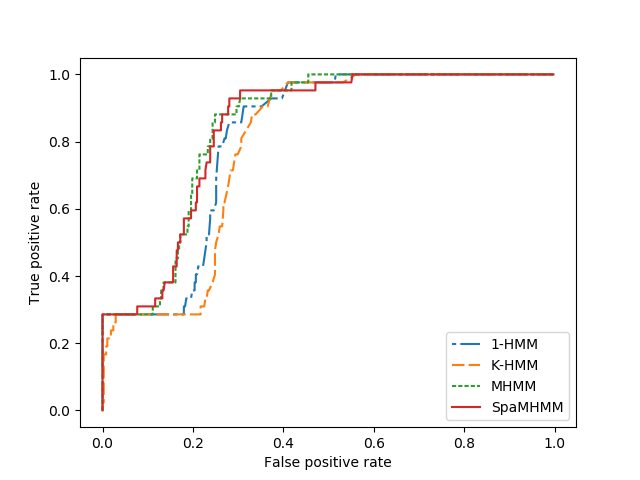
\includegraphics[width=0.8\linewidth]{ChapterTwo/roc.png}
	\caption{ROC curves for each model on the Wi-Fi dataset, for one of the 10 runs.}
	\label{fig:roc}
\end{figure}

\begin{table}
	\centering
	\begin{tabular}{l|r|r r}
		\multicolumn{1}{c}{} & \multicolumn{1}{c}{} & \multicolumn{2}{c}{Average log-likelihood} \\
		& \multicolumn{1}{c|}{AUC} & Normal data & Anomalous data \\
		\hline
		1-HMM & $0.806~(\pm 0.01)$ & $-6.36~(\pm 0.66)$ & $-129.40~(\pm 22.22)$ \\
		K-HMM & $0.776~(\pm 0.01)$ & $-22.09~(\pm 1.12)$ & $\mathbf{-130.36}~(\pm 26.30)$ \\
		MHMM & $\mathbf{0.830}~(\pm 0.01)$ & $-3.31~(\pm 0.21)$ & $-10.99~(\pm 1.10)$ \\
		SpaMHMM & $0.829~(\pm 0.01)$ & $\mathbf{-3.26}~(\pm 0.12)$ & $-11.29~(\pm 1.39)$ \\
	\end{tabular}
	\caption{AUC and average log-likelihood per sample for each model in the Wi-Fi dataset averaged over 10 training runs. Standard deviations are in brackets. Best results are in bold.}
	\label{tbl:wifi_results}
\end{table}

\subsection{Human motion forecasting}
\label{sec:h36m}
The human body is constituted by several interdependent parts, which interact as a whole producing sensible global motion patterns. These patterns may correspond to multiple activities like walking, eating, etc. Here, we use our model to make short-time prediction of sequences of human joint positions, represented as motion capture (mocap) data. The current state of the art methodologies use architectures based on deep recurrent neural networks (RNNs), achieving remarkable results both in short-time prediction \citet{Fragkiadaki2015, Martinez2017} and in long-term motion generation \citet{Jain2016, Pavllo2018}.

Our experiments were conducted on the Human3.6M dataset from \citet{Ionescu2011, Ionescu2014}, which consists of mocap data from 7 subjects performing 15 distinct actions. In this experiment, we have considered only 4 of those actions, namely ``walking'', ``eating'', ``smoking'' and ``discussion''. There, the human skeleton is represented with 32 joints whose position is recorded at 50 Hz. We build our 32x32-dimensional symmetric matrix $\mG$ representing the graph $\gG$ in the following sensible manner: $G_{j,k}=1$, if there is an actual skeleton connection between joints $j$ and $k$ (e.g.\  the elbow joint is connected to the wrist joint by the forearm); $G_{j,k}=1$, if joints $j$ and $k$ are symmetric (e.g.\  left and right elbows); $G_{j,k}=0$, otherwise.

\subsubsection{Forecasting}

We reproduced as much as possible the experimental setup followed in \citet{Fragkiadaki2015}. Specifically, we down-sampled the data by a factor of 2 and transformed the raw 3-D angles into an exponential map representation. We removed joints with constant exponential map, yielding a dataset with 22 distinct joints, and pruned our matrix $\mG$ accordingly. Training was performed using data from 6 subjects, leaving one subject (denoted in the dataset by ``S5'') for testing. We did 3-fold cross-validation on the training data of the action ``walking'' to find the optimal number of mixture components $M$ and hidden states $S$ for the baseline mixture MHMM. Unsurprisingly, since this model can hardly overfit in such a complex task, we ended up with $M=18$ and $S=12$, which were the largest values in the ranges we defined. Larger values are likely to improve the results, but the training time would become too large to be practical. For SpaMHMM, we used these same values of $M$ and $S$ and we did 3-fold cross validation on the training data of the action ``walking'' to fine-tune the value of $\reg$ in the range $[10^{-4}, 1]$. We ended up using $\reg=0.05$. The number of hidden states in 1-HMM was set to 51 and in K-HMM it was set to 11 hidden states per HMM. The same values were then used to train the models for the remaining actions. Every model was trained for 100 iterations of EM  or until the loss plateaus. For SpaMHMM, we did 100 iterations of the inner loop on each M-step, using a learning rate $\rho=10^{-2}$.

In order to generate predictions for a joint (node) $y$ starting from a given prefix sequence $\mX_{\text{pref}}$, we compute the posterior distribution $p(\rmX | \mX_{\text{pref}}, y)$ (see details in \Secref{sec:posterior_proof}) and we sample sequences from that posterior. Our evaluation method and metric again followed \citet{Fragkiadaki2015}. We fed our model with 8 prefix subsequences with 50 frames each (corresponding to 2 seconds) for each joint from the test subject and we predicted the following 10 frames (corresponding to 400 miliseconds). Each prediction was built by sampling 100 sequences from the posterior and averaging. We then computed the average mean angle error for the 8 sequences at different time horizons. 

Results are in \Tableref{tbl:h36m_results}. Among our models (1-HMM, K-HMM, MHMM and SpaMHMM), SpaMHMM outperformed the remaining in all actions except ``eating''. For this action in particular, MHMM was slightly better than SpaMHMM, probably due to the lack of symmetry between the right and left sides of the body, which was one of the prior assumptions that we have used to build the graph $\gG$. ``Smoking'' and ``discussion'' activities may also be highly non-symmetric, but results in our and others' models show that these activities are generally harder to predict than ``walking'' and ``eating'. Thus, here, the skeleton structure information encoded in $\gG$ behaves as a useful prior for SpaMHMM, guiding it towards better solutions than MHMM. The worse results for 1-HMM and K-HMM likely result from the same limitations that we have pointed out in \Secref{sec:wi_fi}: each component in K-HMM is inherently trained with less data than the remaining models, while 1-HMM does not make distinction between different graph nodes. Extending the discussion to the state of the art solutions for this problem, we note that SpaMHMM compares favorably with ERD, LSTM-3LR and SRNN, which are all RNN-based architectures. Moreover, ERD and LSTM-3LR were designed specifically for this task, which is not the case for SpaMHMM. This is also true for GRU supervised and QuaterNet, which clearly outperform all remaining models, including ours. This is unsurprising, since RNNs are capable of modeling more complex dynamics than HMMs, due to their intrinsic non-linearity and continuous state representation. This also allows their usage for long-term motion generation, in which HMMs do not behave well due their linear dynamics and lack of long-term memory. However, unlike GRU supervised and QuaterNet, SpaMHMM  models the probability distribution of the data directly, allowing its application in domains like novelty detection. Regarding sparsity, the experiments confirm that the SpaMHMM mixture coefficients are actually sparser than those of MHMM, as shown in \Figref{fig:sparsity}.

\begin{table*}
	\resizebox{\textwidth}{!}{
		\begin{tabular}{l|c c c c| c c c c| c c c c | c c c c}
			\multicolumn{1}{c}{} & \multicolumn{4}{c}{Walking} & \multicolumn{4}{c}{Eating} & \multicolumn{4}{c}{Smoking} & \multicolumn{4}{c}{Discussion} \\
			miliseconds & 80 & 160 & 320 & 400 & 80 & 160 & 320 & 400 & 80 & 160 & 320 & 400 & 80 & 160 & 320 & 400 \\
			\hline
			1-HMM & 0.91 & 1.04 & 1.22 & 1.31 & 1.00 & 1.08 & 1.15 & 1.21 & 1.45 & 1.55 & 1.70 & 1.75 & 1.19 & 1.42 & 1.55 & 1.56 \\
			K-HMM & 1.29 & 1.33 & 1.34 & 1.38 & 1.16 & 1.22 & 1.28 & 1.34 & 1.70 & 1.77 & 1.90 & 1.95 & 1.47 & 1.61 & 1.68 & 1.63 \\
			MHMM & \textbf{0.78} & \textbf{0.93} & 1.13 & 1.21 & \textbf{0.77} & \textbf{0.87} & \textbf{0.98} & \textbf{1.06} & 1.44 & 1.53 & 1.69 & 1.77 & 1.14 & 1.36 & 1.52 & 1.54 \\
			SpaMHMM & 0.80 & \textbf{0.93} & \textbf{1.11} & \textbf{1.18} & 0.81 & 0.90 & 0.99 & \textbf{1.06} & \textbf{1.29} & \textbf{1.39} & \textbf{1.61} & \textbf{1.67} & \textbf{1.09} & \textbf{1.30} & \textbf{1.44} & \textbf{1.49} \\
			\hline
			ERD \citet{Fragkiadaki2015} & 0.93 & 1.18 & 1.59 & 1.78 & 1.27 & 1.45 & 1.66 & 1.80 & 1.66 & 1.95 & 2.35 & 2.42 & 2.27 & 2.47 & 2.68 & 2.76 \\
			LSTM-3LR \citet{Fragkiadaki2015} & 0.77 & 1.00 & 1.29 & 1.47 & 0.89 & 1.09 & 1.35 & 1.46 & 1.34 & 1.65 & 2.04 & 2.16 & 1.88 & 2.12 & 2.25 & 2.23 \\
			SRNN \citet{Jain2016} & 0.81 & 0.94 & 1.16 & 1.30 & 0.97 & 1.14 & 1.35 & 1.46 & 1.45 & 1.68 & 1.94 & 2.08 & 1.22 & 1.49 & 1.83 & 1.93 \\
			GRU sup. \citet{Martinez2017} & 0.28 & 0.49 & 0.72 & 0.81 & 0.23 & 0.39 & 0.62 & 0.76 & 0.33 & 0.61 & 1.05 & 1.15 & 0.31 & 0.68 & 1.01 & 1.09 \\
			QuaterNet \citet{Pavllo2018} & \underline{0.21} & \underline{0.34} & \underline{0.56} & \underline{0.62} & \underline{0.20} & \underline{0.35} & \underline{0.58} & \underline{0.70} & \underline{0.25} & \underline{0.47} & \underline{0.93} & \underline{0.90} & \underline{0.26} & \underline{0.60} & \underline{0.85} & \underline{0.93}
	\end{tabular}}
	\caption{Mean angle error for short-term motion prediction on Human3.6M for different actions and time horizons. The results for ERD, LSTM-3LR, SRNN, GRU supervised and QuaterNet were extracted from \citet{Pavllo2018}. Best results among our models are in bold, best overall results are underlined.}
	\label{tbl:h36m_results}
\end{table*}

\begin{figure}
	\centering
	\begin{minipage}{.3\textwidth}
		\centering
		\begin{tikzpicture}
			\begin{axis}[
			ybar,
			bar width=10pt,
			width=120pt,
			height=180pt,
			xmin=Wi-Fi, xmax=Wi-Fi,
			symbolic x coords={Wi-Fi},
			xtick=data,
			ylabel=Sparsity,
			ymin=0, ymax=1,
			ymajorgrids,
			major grid style={dashed},
			yminorgrids,
			minor grid style={dashed},
			minor tick num=1,
			]
			\addplot[fill=white, error bars/.cd, y dir=both, y explicit] 
			coordinates {(Wi-Fi, 0.749) +- (Wi-Fi, 0.017)};
			\addplot[fill=lightgray, error bars/.cd, y dir=both, y explicit] 
			coordinates {(Wi-Fi, 0.755) +- (Wi-Fi, 0.022)};
			\legend{}
			\end{axis}
		\end{tikzpicture}
	\end{minipage}%
	\begin{minipage}{.7\textwidth}
		\centering
		\begin{tikzpicture}
			\begin{axis}[
			ybar,
			bar width=10pt,
			width=250pt,
			height=180pt,
			symbolic x coords={Walking,Eating,Smoking,Discussion},
			xtick=data,
			ymin=0, ymax=1,
			ymajorgrids,
			major grid style={dashed},
			yminorgrids,
			minor grid style={dashed},
			minor tick num=1,
			legend style={at={(0.75,0.9)},
				anchor=north,legend columns=1},
			]
			\addplot[fill=white] 
			coordinates {(Walking,0.535) (Eating,0.465) (Smoking,0.343) (Discussion,0.455)};
			\addplot[fill=lightgray] 
			coordinates {(Walking,0.576) (Eating,0.540) (Smoking,0.457) (Discussion,0.533)};
			\legend{MHMM,SpaMHMM}
			\end{axis}
		\end{tikzpicture}
	\end{minipage} 
	\caption{Relative sparsity (number of coefficients equal to zero / total number of coefficients) of the obtained MHMM and SpaMHMM models on the Wi-Fi dataset (left) and on the Human3.6M dataset for different actions (right). For the Wi-Fi dataset, the average value over the 10 training runs is shown together with the standard deviation. Both models for the Wi-Fi dataset have 150 coefficients. All models for the Human3.6M dataset have 396 coefficients.}
	\label{fig:sparsity}
\end{figure}

\subsubsection{Joint cluster analysis}
\label{sec:spamhmm_cluster}
We may roughly divide the human body in four distinct parts: upper body (head, neck and shoulders), arms, torso and legs. Joints that belong to the same part naturally tend to have coherent motion, so we would expect them to be described by more or less the same components in our mixture models (MHMM and SpaMHMM). Since SpaMHMM is trained to exploit the known skeleton structure, this effect should be even more apparent in SpaMHMM than in MHMM. In order to confirm this conjecture, we have trained MHMM and SpaMHMM for the action ``walking'' using four mixture components only, i.e.\ $M=4$, and we have looked for the most likely component (cluster) for each joint:
\begin{equation}
C_k = \argmax_{m \in \{1,...,M\}} p(\rz=m | \ry=k) = \argmax_{m \in \{1,...,M\}} \alpha_{k,m},
\end{equation}
where $C_k$ is, therefore, the cluster assigned to joint $k$. The results are in \Figref{fig:clusters}. From there we can see that MHMM somehow succeeds on dividing the body in two main parts, by assigning the joints in the torso and in the upper body mostly to the red/'+' cluster, while those in the hips, legs and feet are almost all assigned to the green/`\SmallTriangleUp' cluster. Besides, we see that in the vast majority of the cases, symmetric joints are assigned to the same cluster. These observations confirm that we have chosen the graph $\gG$ for this problem in an appropriate manner. However, some assignments are unnatural: e.g.\  one of the joints in the left foot is assigned to the red/`+' cluster and the blue/`$\circ$' cluster is assigned to one single joint, in the left forearm. We also observe that the distribution of joints per clusters is highly uneven, being the green/`\SmallTriangleUp' cluster the most represented by far. SpaMHMM, on the other hand, succeeds on dividing the body in four meaningful regions: upper body and upper spine in the green/`\SmallTriangleUp' cluster; arms in the blue/`$\circ$' cluster; lower spine and hips in the orange/`x' cluster; legs and feet in the red/`+' cluster. Note that the graph $\gG$ used to regularize SpaMHMM does not include any information about the body part that a joint belongs to, but only about the joints that connect to it and that are symmetric to it. Nevertheless, the model is capable of using this information together with the training data in order to divide the skeleton in an intuitive and natural way. Moreover, the distribution of joints per cluster is much more even in this case, what may also help to explain why SpaMHMM outperforms MHMM: by splitting the joints more or less evenly by the different HMMs in the mixture, none of the HMM components is forced to learn too many motion patterns. In MHMM, we see that the green/`+' component, for instance, is the most responsible to model the motion of almost all joints in the legs and hips and also some joints in the arms and the red/`+' component is the prevalent on the prediction of the motion patterns of the neck and left foot, which are presumably very different.

\begin{figure*}
	\centering
	\begin{minipage}{.5\textwidth}
		\centering
		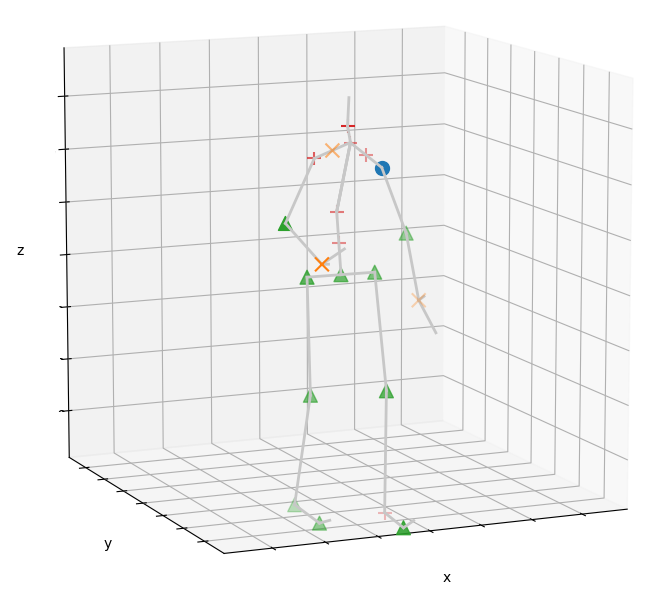
\includegraphics[width=0.8\linewidth]{ChapterTwo/mhmm_clusters}
	\end{minipage}%
	\begin{minipage}{.5\textwidth}
		\centering
		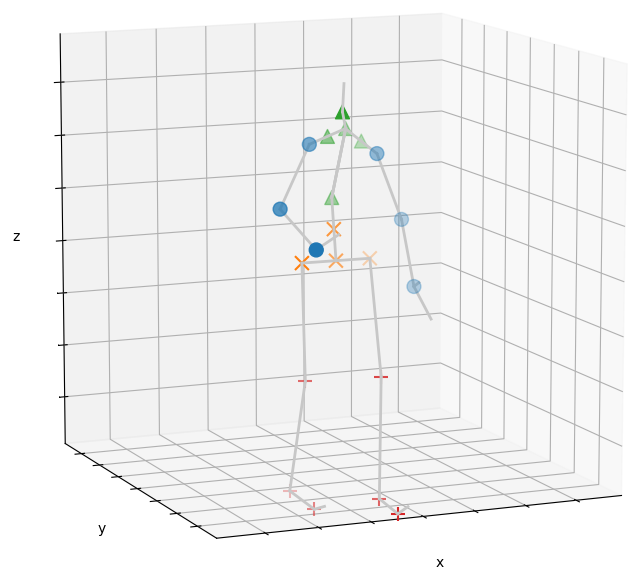
\includegraphics[width=0.8\linewidth]{ChapterTwo/spamhmm_clusters}
	\end{minipage}
	\caption{Assignments of joints to clusters in MHMM (left) and SpaMHMM (right). The different colors (blue, green, orange, red) and the respective symbols (`$\circ$', `\SmallTriangleUp', `x', `+') on each joint represent the cluster that the joint was assigned to. on each joint represent the cluster that the joint was assigned to.}
	\label{fig:clusters}
\end{figure*}

% Chapter Template

% Main chapter title
%\chapter[toc version]{doc version}
\chapter{Multi-source domain adaptation}

% Short version of the title for the header
%\chaptermark{version for header}

% Chapter Label
% For referencing this chapter elsewhere, use \ref{ChapterTemplate}
\label{chp:domain_adaptation}

% Write text in here
% Use \subsection and \subsubsection to organize text

\begin{tcolorbox}
	\small{
		Some parts of this chapter were originally published in or adapted from:
		\begin{itemize}
			\item[] \cite{ThesisFrancisco} \bibentry{ThesisFrancisco} (presented in \Secref{sec:da_sensors})
			\item[] \cite{MODAFM} \bibentry{MODAFM} (presented in \Secref{sec:modafm})
		\end{itemize}
		
		The Master's thesis \cite{ThesisFrancisco} was supervised by Jaime S. Cardoso and co-supervised by Diogo Pernes.
	}
\end{tcolorbox}

\section{Introduction}
\label{sec:chp3_intro}
In Chapter \ref{chp:networked_data_streams}, we have addressed the situation where the set of entities was the same at training and testing time. The goal there was to exploit inter-correlations between entities to learn better generative models for each individual entity. Now, we focus on the problem of learning a discriminative model for one particular entity (the \newterm{target}) for which no annotated data is available. Assuming some invariance properties, we can hope to accomplish this task by learning a discriminative model using the combination of annotated data from the remaining entities (the \newterm{sources}) and unlabeled data from the target entity. Since entities do not need to (and generally do not) correspond to physical objects and may refer to different contexts where the data was collected, they are more commonly called \newterm{domains} and the problem itself is known as \newterm{domain adaptation} (DA). In the following, we motivate the practical importance of this problem and summarize our contributions.

Supervised training of deep neural networks has achieved outstanding results on multiple learning tasks greatly due to the availability of large and rich annotated datasets. Unfortunately, annotating such large-scale datasets is often prohibitively time-consuming and expensive. Furthermore, in many practical cases, it is not possible to collect annotated data with the same characteristics as the test data, and, as a result, training and test data are drawn from distinct underlying distributions. As a consequence, the model performance tends to decrease significantly on the test data. The goal of DA algorithms is to minimize this gap by finding transferable knowledge from the source to the target domain. Sometimes, it is assumed that a small portion of labeled target data are available at training time -- a setting that is known as \newterm{semi-supervised} DA (e.g.\ \citet{Daume2010, Donahue2013, Kumar2010, Saito2019, Yao2015}). In this chapter, we focus mostly on the more challenging scenario, where no labeled target data are available for training -- known as \newterm{unsupervised} DA (e.g.\ \citet{Baktashmotlagh2013, Ganin2015, Kang2019, Long2016, Zhao2018}). The DA problem, in its semi-supervised and unsupervised variants, has received increased attention in recent years, both from theoretical (e.g.\ \citet{BenDavid2010, BenDavid2007, Blitzer2008, Cortes2014, Gopalan2013, Hoffman2018, Zhao2019}) and algorithmic perspectives (e.g.\ \citet{Ajakan2014, Becker2013, Fernando2013, Jhuo2012, Long2015, Louizos2015, Sun2016, Tzeng2017}). In many situations, the annotated training data may consist of a combination of distinct datasets, some of which may be closer or further away from the target data. Finding nontrivial ways of combining multiple datasets to approximate the target distribution and extracting relevant knowledge from such combination is the purpose of multi-source DA algorithms (e.g.\ \citet{Kim2017, Guo2018, Hoffman2018, Mansour2009, Sebag2019, Zhang2015, Zhao2018}) and is also our main focus in this chapter.

The remainder of the chapter is organized as follows: i) we formalize the problem and provide some useful background by reviewing some important theoretical results and state of the art algorithms (\Secref{sec:chp3_background}); ii) we discuss some exploratory solutions for this problem in the context of sensor networks (\Secref{sec:da_sensors}); and finally iii) we present our own novel algorithm for multi-source domain adaptation (\Secref{sec:modafm}).

\section{Background}
\label{sec:chp3_background}
We start by analyzing the problem of DA from a theoretical perspective and then we overview the main approaches that constitute the state of the art. Although some authors have considered the problem of DA for regression problems (e.g.\ \cite{Cortes2011}, \cite{Zhao2018}), the literature on classification is far more vast. Moreover, many of the results and methods explained in this section can be extended to regression problems with minor modifications. For these reasons, we shall focus our discussion mostly on classification.

\subsection{Theoretical foundation}
\label{sec:da_theory}

\subsubsection{Single source setting}
\label{sec:da_theory_ss}
\citet{BenDavid2010} developed a rigorous yet comprehensive theoretical model for domain adaptation that we summarize here. This formulation enlightens the intrinsic difficulties associated with this task and provides a deep foundation for many of the algorithms we discuss in this chapter and, particularly, to our own approach, presented in \Secref{sec:modafm}.

Before we present and discuss the most important results, let us introduce a few preliminary definitions. A \newterm{domain} $\gD$ is defined by a joint distribution $p_\gD(\rvx, \rvy)$ over input features $\rvx \in \gX$ and target variables $\rvy \in \gY$, where $\gX$ and $\gY$ denote the input and target spaces, respectively. For the domain adaptation task to be well defined, at least two domains must be considered: a \newterm{source} domain $\gS$, with joint distribution denoted by $p_\gS(\rvx, \rvy)$, from which abundant annotated data is usually available, and a \newterm{target} domain $\gT$, with joint distribution $p_\gT(\rvx, \rvy)$, from which scarce or even zero annotated data is available at training time. Following most classical results from statistical learning theory, \citet{BenDavid2010} focused on binary classification, thus $\gY = \{0, 1\}$. Under this setting, it is possible to define a \newterm{labeling function} $f_\gD: \gX \mapsto [0, 1]$ for each domain, given by $f_\gD(\vx) = p_\gD(\ry=1 \mid \vx)$. A \newterm{hypothesis} is any function $h: \gX \mapsto \{0,1\}$ and a set $\gH$ of these functions is called a \newterm{hypothesis class}. The expected absolute difference between $h$ and $f_\gD$ is called the \newterm{risk} (or \newterm{error}) of hypothesis $h$ (with respect to the labeling function $f_\gD$):
\begin{equation}
	\label{eq:risk}
	\epsilon(h,f_\gD) \triangleq \E_{\rvx \sim p_\gD} |h(\rvx) - f_\gD(\rvx)|.
\end{equation}
We use $\epsilon_\gS(h)$ and $\epsilon_\gT(h)$ as shorthands for $\epsilon(h,f_\gS)$ and $\epsilon(h,f_\gT)$ and refer to them as the source and target risks (or errors), respectively. The empirical estimates of these are denoted as $\widehat{\epsilon}_\gS(h)$ and $\widehat{\epsilon}_\gT(h)$, respectively.

Given two domains $\gD$ and $\gD'$ and a hypothesis class $\gH$, the $\gH$-divergence provides a distance measure between the marginal distributions of features in $\gD$ and $\gD'$ (according to $\gH$):
\begin{equation*}
	\label{eq:h_div}
	d_{\gH}(\gD,\gD') \triangleq \sup_{h \in \gH} 2 |\mathrm{Pr}_{\gD}(\1_h) - \mathrm{Pr}_{\gD'}(\1_h)|,
\end{equation*}
where $\1_h \triangleq \{\vx \in \gX: h(\vx)=1\}$ and $\mathrm{Pr}_{\gD}(\1_h)$ is the probability assigned by the distribution $p_\gD(\rvx)$ to the subset $\1_h \subseteq \gX$. As is often the case, when the true underlying marginal distributions are unknown or intractable but finite sets of (unlabeled) samples from both domains are available, an empirical $\gH$-divergence can be constructed by replacing the true probabilities $\mathrm{Pr}_{\gD}(\1_h)$ and $\mathrm{Pr}_{\gD'}(\1_h)$ by the respective empirical estimates. Remarkably, under weak conditions on the hypothesis class, computing this empirical $\gH$-divergence is equivalent to finding the hypothesis in $\gH$ that maximally discriminates between samples of the two domains. This result is enunciated formally in Lemma \ref{lemma:emp_h_div} and, as we shall see later, is exploited by adversarial-based approaches for domain adaptation.
\begin{lemma}
	\label{lemma:emp_h_div}
	(Lemma 2 from \citet{BenDavid2010}) Let $\gH$ be a hypothesis class such that if $h \in \gH$ then $1-h \in \gH$. Given two sets $\widehat{D}$ and $\widehat{D}'$ of $n$ samples each drawn from two domains $D$ and $D'$, the empirical $\gH$-divergence between $D$ and $D'$ is given by:
	\begin{equation}
		\widehat{d}_{\gH}(\gD,\gD') = 2 \left(1 - \min_{h \in \gH} \left[\frac{1}{n} \sum_{\vx: h(\vx)=1} \1_{\vx \in \widehat{\gD}} + \frac{1}{n} \sum_{\vx: h(\vx)=0} \1_{\vx \in \widehat{\gD}'}\right]\right).
	\end{equation}
\end{lemma}
Note that if the two sets $\widehat{\gD}$ and $\widehat{\gD}'$ can be discriminated perfectly by a hypothesis $h \in \gH$ (i.e.\ if there is an $h \in \gH$ such that $h(\vx) = 0$ if $x \in \widehat{\gD}$ and $h(\vx) = 1$ if $x \in \widehat{\gD}'$), then $\widehat{d}_{\gH}(\gD,\gD')$ is maximum and equal to 2.

For a hypothesis class $\gH$, we may define the \newterm{symmetric difference hypothesis class} $\gH \Delta \gH$ as:
\begin{equation}
\label{eq:h_delta_h}
\gH \Delta \gH \triangleq \{l: l(\vx) = h(\vx) \oplus h'(\vx), \; h, h' \in \gH\},
\end{equation}
where $\oplus$ denotes the ``exclusive or" (xor) operation. Combining this definition with \eqref{eq:h_div}, the definition of $\gH \Delta \gH$-divergence, which happens to play a major role in Theorem \ref{thm:da_bound_single_source}, follows immediately. This theorem is the main result in this section as it provides an upper bound for the target risk given the source risk and the $\gH \Delta \gH$-divergence between the source and target domains.
\begin{theorem}
	\label{thm:da_bound_single_source} (Theorem 2 from \citet{BenDavid2010}) Let $\gH$ be a hypothesis class with VC-dimension $d$. Consider $n$ unlabeled samples drawn from each of the two domains $\gS$ (source) and $\gT$ (target). Then, for every $h \in \gH$ and any $\delta \in (0,1)$, with probability at least $1-\delta$ over the choice of samples,
	\begin{equation}
		\label{eq:da_bound_single_source}
		\epsilon_\gT(h) \leq \epsilon_\gS(h) + \frac{1}{2} \widehat{d}_{\gH \Delta \gH}(\gS, \gT) + \lambda + 2\sqrt{\frac{2d\log(2n) + \log(\frac{2}{\delta})}{n}},
	\end{equation}
	where $\lambda \triangleq \min_{h \in \gH} \epsilon_\gS(h) + \epsilon_\gT(h)$.
\end{theorem}
This bound immediately confirms the intuition that a low target error can be achieved by training a classifier to minimize the error in the source domain, provided that the marginal distributions of features are similar (i.e.\ $\widehat{d}_{\gH \Delta \gH}(\gS, \gT)$ is small) and a low error on the combination of the two domains can be achieved (i.e.\ $\lambda$ is also small). A deeper and more complete interpretation of this bound shall be provided later on, when we take into account the fact that, by applying deep neural networks, we can not only construct rich hypothesis classes but also manipulate and learn feature representations. The latter observation suggests that this kind of the classifiers may also have an impact on the $\widehat{d}_{\gH \Delta \gH}(\gS, \gT)$ and $\lambda$ terms in \eqref{eq:da_bound_single_source}, which will indeed be the case.

\subsubsection{Multi-source setting}
\label{sec:da_theory_ms}
So far we have only considered the setting where a single source domain was available. However, in many practical cases, the annotated training dataset consists of a collection of subdatasets, each one belonging to its own domain. Therefore, it makes sense to consider $k$ distinct source domains $\gS_1, \gS_2, \dots, \gS_k$ and, in particular, to see how Theorem \ref{thm:da_bound_single_source} can be generalized to this setting.
\begin{theorem}
	\label{thm:da_bound_multi_source}
	(Theorem 2 from \citet{Zhao2018}) Let $\gH$ be a hypothesis class with VC-dimension $d$. Consider $n$ unlabeled samples drawn from the target domain $\gT$ and $n/k$ annotated samples drawn from each of the $k$ source domains $\gS_1, \gS_2, \dots, \gS_k$. Then, for every $h \in \gH$, any $\valpha \in [0,1]^k: \sum_{j=1}^k \evalpha_i = 1$, and any $\delta \in (0,1)$, with probability at least $1-\delta$ over the choice of samples,
	\begin{equation}
		\label{eq:da_bound_multi_source}
		\epsilon_\gT(h) \leq \sum_{j=1}^k \evalpha_j \left(\widehat{\epsilon}_{\gS_j}(h) + \frac{1}{2} \widehat{d}_{\gH \Delta \gH}(\gS_j, \gT)\right) + \lambda_\valpha + O \left(\sqrt{\frac{1}{n} \left(\log \frac{1}{\delta} +d \log \frac{n}{d} \right)} \right),
	\end{equation}
	where $\lambda_\valpha \triangleq \min_{h \in \gH} \epsilon_\gT(h) + \sum_{j=1}^k \evalpha_j \epsilon_{\gS_j}(h)$.
\end{theorem}
Unsurprisingly, the bound in Theorem \ref{thm:da_bound_multi_source} is essentially a convex combination of the bounds provided by Theorem \ref{thm:da_bound_single_source} for each individual source domain. Thus, the same interpretation applies here. Nonetheless, the source weights $\valpha$ provide an extra degree of freedom that should be taken into account. Depending on how much each source domain differs from the target, it may be beneficial to weight each source domain differently. Adjusting these weights is therefore an extra non-trivial task, exclusive to the multi-source setting, that may have a significant impact in the performance of the domain adaptation algorithm.

\subsection{State of the art}
\label{sec:da_sota}
We now do a brief overview of the most relevant DA algorithms, both in the single source and multi-source settings. 

As we have just seen from a theoretical point of view, the success of the DA task depends on how similar the target domain is to the source(s), which is equivalent to saying that some properties of the underlying distributions must be invariant across domains. Different DA algorithms can therefore be categorized according to the invariance properties they assume.

\subsubsection{Target shift}
\label{sec:target_shift_sota}
\begin{figure}
	\centering
	\begin{tikzpicture}[every loop/.style={},thick,
		main node/.style={circle,draw},font=\sffamily\Large\bfseries]
		
		\node[main node,minimum size=1.5cm] (D) {$\gD$};
		\node[main node,minimum size=1.5cm] (y) [right=1.5cm of D] {$\ry$};
		\node[main node,minimum size=1.5cm] (x) [right=1.5cm of y] {$\rvx$};
		
		\draw[->]
		(D) edge (y)
		(y) edge (x);
		
	\end{tikzpicture}
	\caption{Graphical representation of the target shift setting as a Bayesian network.}
	\label{fig:target_shift}
\end{figure}
In the \newterm{target shift} setting, only the marginal distribution of labels is allowed to vary across domains. A practical example where this assumption may be realistic is when the label $\ry$ represents having or not a certain disease and the input features $\rvx$ are symptoms. It is plausible to assume that the prevalence of the disease may vary over time or across different populations, but the probability of some symptom being present or absent given that one has or not the disease should remain constant. Thus, as represented in \Figref{fig:target_shift}, the joint distribution of any domain $\gD$ is assumed to factorize as $p_\gD(\rvx, \ry) = p(\rvx \mid \ry) p_\gD(\ry)$, where $p(\rvx \mid \ry)$ is domain-invariant. By further assuming that $\mathrm{Supp}(p_\gT(\ry)) \subseteq \mathrm{Supp}(p_\gS(\ry))$, we have:
\begin{align}
	p_\gT(\ry \mid \rvx) &\propto p(\rvx \mid \ry) p_\gT(\ry) \nonumber\\
	&= p(\rvx \mid \ry) p_\gS(\ry) \frac{p_\gT(\ry)}{p_\gS(\ry)} \nonumber\\
	&\propto p_\gS(\ry \mid \rvx) \frac{p_\gT(\ry)}{p_\gS(\ry)}.
\end{align}
Thus, if the class ratios $p_\gT(\ry)/p_\gS(\ry)$ are known, the problem of DA under target shift is solved by learning a probabilistic classifier on the source domain, reweighting it with the class ratios, and then normalizing the class scores. Therefore, the literature for DA under target shift focuses on estimating class ratios when these are unknown and cannot be estimated directly from the training data, due to the absence of labels for the target samples.

An elegant and simple solution for this problem was proposed by \citet{Lipton2018}. Specifically, for any classifier $h: \gX \mapsto \gY$ trained with labeled data from the source domain, the target shift assumption implies that $p_{\gT}(h(\rvx) \mid \ry) = p_{\gS}(h(\rvx) \mid \ry)$ and hence:
\begin{align}
p_{\gT}(h(\rvx)) &= \sum_{\ry} p_{\gT}(h(\rvx) \mid \ry) p_{\gT}(\ry) \nonumber\\
\allowdisplaybreaks
&= \sum_{\ry} p_{\gS}(h(\rvx) \mid \ry) p_{\gT}(\ry) \label{eq:estim_class_dist}\\
\allowdisplaybreaks
&= \sum_{\ry} p_{\gS}(h(\rvx), \ry) \frac{p_{\gT}(\ry)}{p_{\gS}(\ry)}. \label{eq:estim_class_ratio}
\end{align}
Note that $p_{\gS}(h(\rvx) \mid \ry)$, $p_{\gS}(h(\rvx), \ry)$, and $p_{\gS}(\ry)$ can all be estimated from labeled source samples and $p_{\gT}(h(\rvx))$ can be estimated from unlabeled target samples. Thus, one can either use \eqref{eq:estim_class_dist} to estimate $p_{\gT}(\ry)$ or \eqref{eq:estim_class_ratio} to estimate class ratios directly.

Other approaches involve learning class-dependent weights to match the mean conditional features of source data with the mean marginal features of target data in a reproducing kernel Hilbert space (e.g.\  \citet{Iyer2004}, \citet{Zhang2013}), or require density estimation to model $p(\rvx \mid \ry)$ (e.g.\ \citet{Chan2005}, \citet{Storkey2009}).

\subsubsection{Conditional shift}
\label{sec:cond_shift_sota}
\begin{figure}
	\centering
	\begin{tikzpicture}[every loop/.style={},thick,
	main node/.style={circle,draw},font=\sffamily\Large\bfseries]
	
	\node[main node,minimum size=1.5cm] (y) {$\ry$};
	\node[main node,minimum size=1.5cm] (x) [right=1.5cm of y] {$\rvx$};
	\node[main node,minimum size=1.5cm] (D) [right=1.5cm of x] {$\gD$};
	
	\draw[->]
	(y) edge (x)
	(D) edge (x);
	
	\end{tikzpicture}
	\caption{Graphical representation of the conditional shift setting as a Bayesian network.}
	\label{fig:cond_shift}
\end{figure}
In the \newterm{conditional shift} setting, the marginal distribution of labels is constant and the conditional of features given labels may change across domains. This scenario is represented in \Figref{fig:cond_shift}, from which it becomes clear that the joint distribution takes the form $p_{\gD}(\rvx, \ry) = p(\ry) p_{\gD}(\rvx \mid \ry)$, where $p(\ry)$ is domain-invariant. Besides being less realistic than other assumptions, DA under conditional shift is in general an ill-posed problem. Nonetheless, \citet{Zhang2013} show that identifiability of $p_{\gT}(\rvx \mid \ry)$ holds when it is assumed that, for any given $y$, $p_{\gT}(\rvx \mid y)$ only differs from $p_{\gS}(\rvx \mid y)$ in location and scale and derive a kernel-based approach to estimate these parameters.

\subsubsection{Concept shift}
\label{sec:concept_shift_sota}
\begin{figure}
	\centering
	\begin{tikzpicture}[every loop/.style={},thick,
	main node/.style={circle,draw},font=\sffamily\Large\bfseries]
	
	\node[main node,minimum size=1.5cm] (x) {$\rvx$};
	\node[main node,minimum size=1.5cm] (y) [right=1.5cm of x] {$\ry$};
	\node[main node,minimum size=1.5cm] (D) [right=1.5cm of y] {$\gD$};
	
	\draw[->]
	(x) edge (y)
	(D) edge (y);
	
	\end{tikzpicture}
	\caption{Graphical representation of the concept shift setting as a Bayesian network.}
	\label{fig:concept_shift}
\end{figure}
\newterm{Concept shift} refers to the situation where the marginal feature distributions $p(\rvx)$ are constant but the conditional distribution of the target variable $p_{\gD}(\ry \mid \rvx)$ is domain-dependent, thus $p_{\gD}(\rvx, \ry) = p(\rvx)p_{\gD}(\ry \mid \rvx)$, as implied by \Figref{fig:concept_shift}. When the change happens over time, this setting is also known as \newterm{concept drift} (\citet{Webb2018}). The literature on concept drift is vast and focuses mostly on the detection of its occurrence so that the model can be updated using new data. \citet{Gama2014} overview the most popular techniques to address this problem.

\subsubsection{Covariate shift}
\label{sec:cov_shift_sota}
\begin{figure}
	\centering
	\begin{tikzpicture}[every loop/.style={},thick,
	main node/.style={circle,draw},font=\sffamily\Large\bfseries]
	
	\node[main node,minimum size=1.5cm] (D) {$\gD$};
	\node[main node,minimum size=1.5cm] (x) [right=1.5cm of D] {$\rvx$};
	\node[main node,minimum size=1.5cm] (y) [right=1.5cm of x] {$\ry$};
	
	\draw[->]
	(D) edge (x)
	(x) edge (y);
	
	\end{tikzpicture}
	\caption{Graphical representation of the covariate shift setting as a Bayesian network.}
	\label{fig:cov_shift}
\end{figure}
\newterm{Covariate shift} is by far the most common assumption and therefore the most widely addressed setting in the DA literature. As implied by the graphical representation in \Figref{fig:cov_shift}, here the conditional distribution of labels given features is constant and the marginal distribution of features is domain-dependent. Thus, $p_\gD(\rvx, \ry) = p(\ry \mid \rvx) p_\gD(\rvx)$, where $p(\ry \mid \rvx)$ is constant across domains. This assumption might hold for instance in image classification problems where the domain shift is caused by different sensors or lighting conditions.

Since $p_\gT(\ry \mid \rvx) = p_\gS(\ry \mid \rvx)$, infinite labeled data from the source domain and a consistent estimator of this conditional distribution would solve this DA task. However, the former is obviously unrealistic and therefore the problem should be analyzed taking into account that the available data is finite. Let $\ell(\cdot, \cdot)$ be any loss function for the supervised learning problem. The goal is then to find an unbiased estimator of the target loss $\E_{\rvx, \ry \sim p_\gT} \ell(h(\rvx),\ry)$ when no labeled samples from the target domain are available. Following \citet{Sugiyama2007}, if the marginal densities $p_\gS(\rvx)$ and $p_\gT(\rvx)$ are known and assuming $\mathrm{Supp}(p_\gT(\rvx)) \subseteq \mathrm{Supp}(p_\gS(\rvx))$, this estimator can be obtained using \newterm{importance weights} $w(\rvx) \triangleq p_\gT(\rvx)/p_\gS(\rvx)$:
\begin{align}
	\E_{\rvx, \ry \sim p_\gT} \ell(h(\rvx),\ry) &= \sum_{\ry} \int l(h(\rvx),\ry) p_\gT(\rvx, \ry) d\rvx \nonumber\\
	&= \sum_{\ry} \int \ell(h(\rvx),\ry) p(\ry \mid \rvx) p_\gT(\rvx) d\rvx \nonumber\\
	&= \sum_{\ry} \int \frac{p_\gT(\rvx)}{p_\gS(\rvx)} \ell(h(\rvx),\ry)  p(\ry \mid \rvx) p_\gS(\rvx) d\rvx \nonumber\\
	&= \sum_{\ry} \int w(\rvx) \ell(h(\rvx),\ry)  p_\gS(\rvx, \ry) d\rvx \nonumber\\
	&= \E_{\rvx, \ry \sim p_\gS} w(\rvx) \ell(h(\rvx),\ry).
\end{align}
Hence, $(1/n) \sum_{i=1}^{n} w(\vx_i) \ell(h(\vx_i),y_i)$ is an unbiased estimator of the target loss, constructed using only source data, which can therefore be used as the loss for the supervised learning problem. When the marginal distributions are unknown and the feature space is low-dimensional, kernel density estimation techniques can be employed to estimate them (e.g.\ \citet{Shimodaira2000,Sugiyama2007,Cortes2010}). An alternative that removes the constraint on the support of the marginal target distribution is learning a transformation $T: \gX \mapsto \gX$ such that $p_{\gS}(T(\rvx)) = p_{\gT}(\rvx)$, which can be accomplished using optimal transport theory (\citet{Courty2015}). Later approaches aim to relax the covariate shift assumption by trying to align the joint source and target distributions (\citet{Courty2017}) and extend the same principles to the multi-source setting (\citet{Turrisi2020}).

For high-dimensional data (e.g.\ images), where the marginal distributions are typically unknown and hard to estimate from finite data, deep learning models play an important role by providing a successful tool learn semantically rich low-dimensional feature representations. It is then possible to learn a function $g:\gX \mapsto \gZ$ mapping input data to a new feature space $\gZ$ such that $p_{\gT}(g(\rvx))/p_{\gS}(g(\rvx)) \approx 1$, i.e.\ where the marginal feature distributions of the two domains coincide. This approach has the additional benefit of moving the overlapping support assumption to a lower-dimensional space, where it is less likely to be violated than in the original space (e.g.\ pixel space). In this new feature space the covariate shift has vanished and therefore any classifier $h:\gZ \mapsto \gY$ that achieves low error on the source domain will also perform well in the target. An alternative way of motivating these approaches follows from analyzing again the target risk bound provided in \eqref{eq:da_bound_single_source}. When we presented this bound, we assumed for simplicity that the feature space was fixed and therefore the upper bound would be minimized by minimizing the source risk. However, if the feature space can itself be optimized, the term $\widehat{d}_{\gH \Delta \gH}(\gS, \gT)$ can be minimized by finding a feature space where the source and target marginal distributions coincide. This idea has been exploited extensively in recent years, either by matching the distributions using maximum mean discrepancy (e.g.\ \citet{Long2015,Guo2018}) or, in most cases, using an adversarial neural network (e.g.\ \citet{Zhao2018,Ganin2015,Pei2018,Sebag2019}).

Adversarial-based DA was originally introduced by \citet{Ganin2015} and results from the observation that 
computing $\widehat{d}_{\gH \Delta \gH}(\gS, \gT)$ is equivalent to finding a classifier that maximally discriminates between samples of the source and target domains (Lemma \ref{lemma:emp_h_div}). Intuitively, if no classifier exists that can distinguish between source and target features, then the distributions of these two must coincide. Thus, if we have access to sets $\widehat{\gS}$ and $\widehat{\gT}$ of labeled samples from the source domain and unlabeled samples from the target, respectively, we can train a feature extractor network $g:\gX \mapsto \gZ$, a classifier $h:\gZ \mapsto \gY$, and a domain discriminator $d:\gZ \mapsto \{0,1\}$ to solve the following minimax problem\footnote{This objective is merely formal since the 0-1 loss is non-smooth and intractable. In practice, the usual classification losses are used instead.}:
\begin{equation}
	\label{eq:dann_obj}
	\min_{g,h} \max_d \quad \widehat{\epsilon}_\gS(h \circ g) + 1 - \left(\frac{1}{n} \sum_{\vx: d(g(\vx))=1} \1_{\vx \in \widehat{\gS}} + \frac{1}{n} \sum_{\vx: d(g(\vx))=0} \1_{\vx \in \widehat{\gT}}\right),
\end{equation}
where $\circ$ denotes function composition. Several variations to this idea have been proposed so far, aiming to extend it to the multi-source setting (\citet{Zhao2018}), or beyond the covariate shift assumption (\citet{Pei2018}), or both (\citet{Sebag2019}).

\subsubsection{Invariance of causal mechanisms}
\label{sec:causal_da_sota}
The settings we have discussed so far consider all features $\rvx$ as atomic and hence do not take into account how different features interact to produce the target variable $\ry$.  Other approaches drop this limitation by decomposing the feature vector into individual features $\rx_1,\rx_2,\dots,\rx_m$, taking into account the structure of the causal Bayesian network governing the data generating process, and using causal inference tools to identify the target distribution. These methods assume that the flow of cause and effect cannot be reversed by domain shift and therefore changes in distribution are due to different interventions in the same causal graph $\gG$ (e.g.\ presence of additional exogenous variables inducing non-causal associations between features and the target variable). \citet{Bareinboim2016} assume $\gG$ is known and all interventions are perfect (i.e.\ all interventions consist of edge removal operations) and derive conditions for identifiability of $p_\gT(\ry \mid \cdots)$ given $\gG$ and $p_\gS(\rvx, \ry)$. \citet{Rojas2018} and \citet{Magliacane2018} relax the covariate shift setting by assuming that there exists a strict subset $\bar{\rvx} \subset \rvx$ such that $p_\gD(\ry \mid \bar{\rvx})$ is domain-invariant and propose algorithms to infer $\bar{\rvx}$ given data from multiple source domains.

Despite being (arguably) more trustworthy than purely data-driven approaches, cau-\allowbreak sality-based methods still struggle to be applied in practice. First of all, they depend to some extent on $\gG$ being given. In many applications, domain knowledge is insufficient to build such a graph. Moreover, causal discovery algorithms, which aim to learn the structure of the graph from data, are computationally expensive and, given observational data, can only recover $\gG$ up to its Markov equivalence class, at least when no parametric assumptions are made  (\citet{Peters2014}). Furthermore, these methods are unsuitable to be applied to image data as no meaningful causal reasoning can be built in pixel space and even deep neural networks are still incapable of finding suitable representations for this goal (\citet{Scholkopf2021}).

\section{Adversarial domain adaptation for object counting in videos}
\label{sec:da_sensors}

\subsection{Motivation}
As different sensors are added to and excluded from a network, we should take into account the fact that the sensors used at training time are different from the ones where the model will make predictions. Since domain shifts between different sensors on a sensor network are usually substantial, it is imperative that robust domain adaptation methods are developed that take into account the constraints of the sensor network.

There is a lack of domain adaptation methods focusing on how to handle the temporal component of data. \citet{Chen2019} proposed an algorithm called Temporal Attentive Alignment for implementing DA in video datasets that explicitly attends to temporal dynamics and \citet{Liu2014} proposed a spatio-temporal DA model named TrCbrBoost for classifying land use. It should be noted, though, that both of these works only deal with a single-source-single-target setting, which is simpler than the multi-source case present when dealing with sensor networks.

For dealing with a multi-source setting, adversarial approaches have proven successful. \citet{Zhao2018} introduced an algorithm called multi-source domain adversarial networks (MDAN) that makes use of $k$ domain discriminators that aim to distinguish between the target and the $k$ source domains. MDAN showed superior performance when compared to other state of the art methods on the task of counting vehicles in images obtained from city cameras videos. Given the positive results obtained, and given the fact that MDAN does not consider the temporal component of the video frames, we consider it is worthy to investigate the adaptation of this model so that it can receive a temporal sequence as an input.

The setting where sensors correspond to video cameras is especially interesting since video data is very high-dimensional. Moreover, the fact that different cameras are located in different places, and therefore have distinct points of view, increases the domain shift and therefore makes this task even more challenging.

Here, we shall explore how to adapt the MDAN model so that both of its adversarial networks are LSTM-based. We decided to go with this type of network since it has already shown promising results in our task: \citet{Zhang2017} introduced an LSTM network architecture for counting vehicles in images obtained from city cameras and reported an improvement of the mean absolute error when compared to other state of the art methods.

\subsection{MDAN: Multi-source domain adversarial networks}
\label{sec:da_sensors_mdan}
We now review the MDAN model introduced by \citet{Zhao2018}. This model is motivated by the target risk bound provided in Theorem \ref{thm:da_bound_multi_source} and is an extension to the multi-source setting of the single source model by \citet{Ganin2015}. Specifically, the following formal objective is considered:
\begin{equation}
	\min_{g,h} \max_{j \in \{1,\cdots,k\}} \quad \widehat{\epsilon}_{\gS_j}(h \circ g) + \frac{1}{2} \widehat{d}_{\gH \Delta \gH}(\gS^g_j, \gT^g),
\end{equation}
where $g: \gX \mapsto \gZ$ and $h: \gZ \mapsto \gY$ are, as before, the feature extractor and the classifier networks and $\gS^g_j$ and $\gT^g$ are, respectively, the $j$-th source domain and the target domain representations in the new feature space $\gZ$ (i.e.\ $p_{\gD^g}(\rvx) \triangleq p_\gD(g(\rvx))$ for any domain $\gD$). Here, the empirical $\gH \Delta \gH$-divergence between $\gS^g_j$ and $\gT^g$ is also implemented with an adversarial domain discriminator $d_j:\gZ \mapsto \{0,1\}$ aiming to discriminate between samples of the two domains. Thus, the model comprises $k$ domain discriminator networks, i.e.\ one for each source domain. This objective is therefore identical to \eqref{eq:dann_obj} with the only difference that, since here there are multiple source domains, the model is optimized for the hardest source domain at each training iteration. In this formulation, $\valpha$ in \eqref{eq:da_bound_multi_source} is a one-hot vector whose active component corresponds to the hardest source domain. Because the bound holds for any convex combination of source domains, the authors also explore a soft-max version of this problem, where smaller positive weights are assigned to the easier source domains:
\begin{equation}
\min_{g,h} \quad \frac{1}{\gamma} \log \sum_{j=1}^{k} \exp \left( \gamma( \widehat{\epsilon}_{\gS_j}(h \circ g) + \frac{1}{2} \widehat{d}_{\gH \Delta \gH}(\gS^g_j, \gT^g)) \right).
\end{equation}
Here, $\gamma > 0$ is a hyperparameter controlling the softness of the max operation ($\gamma \to \infty$ corresponds to the hard-max).

\subsection{FCN-rLSTM: Spatio-temporal deep neural network for object counting}
\label{sec:da_sensors_fcn_rltsm}

\citet{Zhang2017} proposed FCN-rLSTM, a deep neural network architecture for counting vehicles in low-quality videos captured by city cameras that will constitute the backbone of our models. 

Although each video frame contains all the information required to identify the number of vehicles in it, issues with the quality of the collected data can make vehicle counting a difficult problem, namely low resolution, vehicle occlusion, and different vehicle scales, particularly noticeable when the camera is too close to the road. Thus, assuming that the frame rate is sufficiently large when compared to the vehicles speed, leveraging information from the previous frames should help improving the accuracy of the prediction for the current frame. For this reason, FCN-rLSTM combines a fully convolutional network with a recurrent module, which preserves memory from the previous frames in LSTM cells. This is a density-based estimation method, being able to deal well with low frame rates, low resolutions, and vehicle occlusions, but having difficulty in accounting for different vehicle scales.

\begin{figure}
	\centering
	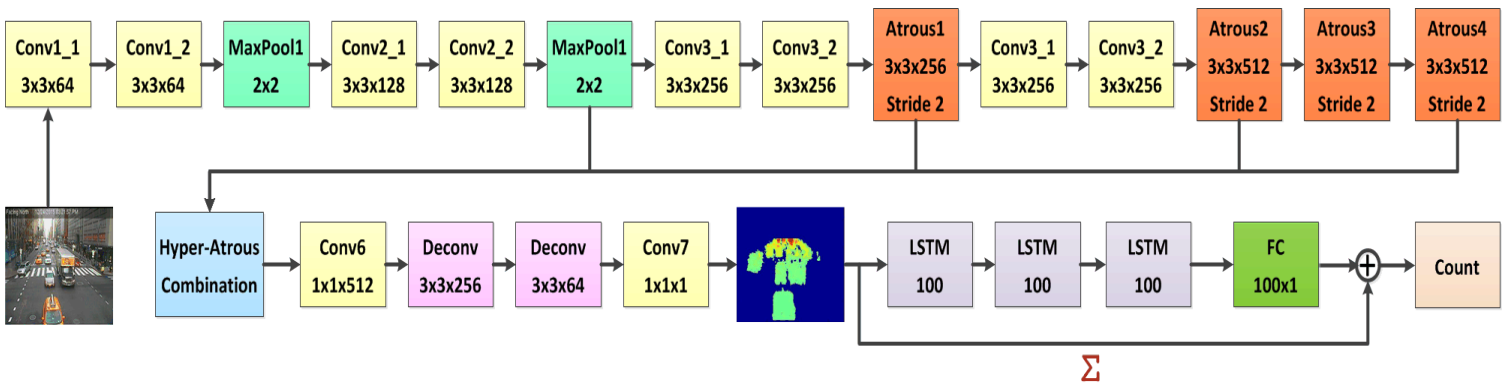
\includegraphics[width=0.9\linewidth]{ChapterThree/fcn_rlstm.png}
	\caption{Architecture of the FCN-rLSTM model (reprinted from \citet{Zhang2017}).}
	\label{fig:fcn_rlstm}
\end{figure}

\Figref{fig:fcn_rlstm} shows the full architecture of this model, from which it can be observed that the convolutional part outputs a density map $\widehat{\mD}$ which is then fed through a recurrent subnetwork responsible for producing the predicted vehicle count $\widehat{y}^{(t)}$. Training this model then implies that each input frame $\mX^{(t)}$ is annotated with the corresponding ground-truth density map $\mD^{(t)}$ and vehicle count $y^{(t)}$. The loss function is defined as:
\begin{equation}
	L(\vtheta) = \frac{1}{n} \sum_{i=1}^{n} ||\widehat{\mD}^{(t)}_i - \mD^{(t)}_i||^2_F + \frac{\lambda_c}{n} \sum_{i=1}^{n} ||\widehat{y}^{(t)}_i - y^{(t)}_i||^2,
\end{equation}
where $||\cdot||_F$ is the Frobenius norm, $\lambda_c > 0$ is a hyperparameter controlling the relative weight of the vehicle counting loss, and the dependency of $\widehat{\mD}^{(t)}_i$ and $\hat{y}^{(t)}_i$ on the network parameters $\vtheta$ is omitted to ease the notation.
% Chapter Template

% Main chapter title
%\chapter[toc version]{doc version}
\chapter{Domain generalization}

% Short version of the title for the header
%\chaptermark{version for header}

% Chapter Label
% For referencing this chapter elsewhere, use \ref{ChapterTemplate}
\label{chp:domain_generalization}

% Write text in here
% Use \subsection and \subsubsection to organize text

\begin{tcolorbox}
	\small{
		Some parts of this chapter were originally published in or adapted from:
		\begin{itemize}
			\item[] \cite{DeSIRe} \bibentry{DeSIRe} (presented in \Secref{sec:desire})
			\item[] \cite{AdvSInvConf} \bibentry{AdvSInvConf} (presented in \Secref{sec:adv_signer_inv})
			\item[] \cite{AdvSInvJournal} \bibentry{AdvSInvJournal} (idem)
			\item[] \cite{AdvInvAttack} \bibentry{AdvInvAttack} (\Secref{sec:adv_inv_attack})
		\end{itemize}

		The first two authors contributed equally in \cite{DeSIRe} and \cite{AdvSInvConf}. Both conceived the models and designed and conducted the experiments, with the supervision of Rebelo and Cardoso. The work in \cite{AdvSInvJournal} extends \cite{AdvSInvConf} by including a more exhaustive experimental evaluation. In \cite{AdvInvAttack}, Diogo Pernes contributed on the development of the proposed methodology, together with the first two authors, who formalized the problem and conducted all experiments. Cardoso supervised the work.
	}
\end{tcolorbox}

\section{Introduction}
\label{sec:chp4_intro}
In Chapters \ref{chp:networked_data_streams} and \ref{chp:domain_adaptation}, the target entities/domains were known at training time. In Chapter \ref{chp:networked_data_streams}, we exploited the correlations between different but related entities to augment the amount of data available for each of those and hence improve the in-distribution generalization. Chapter \ref{chp:domain_adaptation} was dedicated to the problem of domain adaptation, whose purpose is to improve the out-of-distribution (OOD) generalization in a specific target domain for which no labeled data is available.

In this chapter, we shall continue focusing on OOD generalization. However, now, the target domain is unknown and, therefore, no data from this domain is available at training time, neither labeled nor unlabeled. The purpose, then, is to use labeled data from multiple source domains to build a discriminative model that generalizes well to unknown OOD target domains -- a problem known as \emph{domain generalization} (\citet{Blanchard2011, Muandet2013}). Our main assumption to accomplish this goal is that the set of features that are relevant for the learning task are domain-invariant. Formally, we assume that, for each domain $\gD$, there exists a bijection $b_\gD: \gX \mapsto \gZ \times \gW$, where $\gZ$ is the domain-invariant space of features used for classification and $\gW$ are domain-specific auxiliary features carrying no relevant signal for the considered learning task. Thus, for $(\rz, \rw) \triangleq b_\gD(\rvx)$, we assume that $p_\gD(\ry \mid \rx) = p(\ry \mid \rz)$, i.e.\ the optimal classifier for any domain $\gD$ can be reconstructed from features in $\gZ$ and a domain-invariant classifier $p(\ry \mid \rz)$.  This formulation is closely related to the covariate shift assumption for domain adaptation, described in \secref{sec:cov_shift_sota}.

A computer vision application where this problem is particularly relevant is sign language recognition (SLR). Large inter-signer variability in the manual signing process of sign languages is one of the challenges associated with this task. Due to this issue, models trained on data from a given set of signers often fail to generalize well when tested on previously unseen signers. Since, ideally, an SLR system should be able to recognize the gestures of any signer, this problem should be tackled with domain generalization (DG) techniques. For this reason, SLR will be the main application considered in this chapter. Nonetheless, we will also show that the same principles can be applied successfully to develop a fingerprint presentation attack detection method that exhibits robust performance on detecting unseen attacks.

The remainder of this chapter is organized as follows: i) we start by presenting the state of the art for DG (\secref{sec:dg_sota}); ii) we present a novel adversarial-based approach for DG in the context of SLR (\secref{sec:adv_signer_inv}); iii) we show how this methodology can be successfully adapted to address the problem of iris presentation attack detection (\secref{sec:adv_iris_attack}); iv) we present a novel reconstruction-based algorithm for DG (\secref{sec:desire}).

\section{State of the art}
\label{sec:dg_sota}
\citet{Zhou2021} divide the algorithms for domain generalization as heterogeneous and homogeneous, depending on whether the label space varies (heterogeneous DG) or not (homogeneous DG). The former case is also known as \emph{zero-shot} domain generalization and its goal is in general to learn a feature representation that can be used in the target domain to recognize new classes. The latter, which will be the focus of this chapter, is closely related to domain adaptation, so there is a significant intersection between the two. \citet{Albuquerque2019} presented an upper bound for the generalization error that is essentially an upper bound for multi-source domain adaptation, similar to the bound by \citet{Zhao2018} (Theorem~\ref{thm:da_bound_multi_source}) and to our own (Theorem~\ref{thm:target_risk_bound}).

The theoretical proximity between the two problems motivates the existence of similar algorithms to tackle them. As a matter of fact, many algorithms for DG follow the paradigm of domain alignment, which we have discussed extensively in the context of DA. \citet{Li2018} use an adversarial autoencoder and maximum mean discrepancy over its latent space to learn domain-invariant features. \citet{Ghifary2015} address the same problem through a multi-output autoencoder, which is trained to transform samples from one domain into samples from the remaining domains with the same label. \citet{Motiian2017} proposed a unified framework to address the problems of domain adaptation and generalization. They use a contrastive $\normltwo$-loss in the latent space that pushes together samples from different domains and the same class while pulling apart samples from different classes. Several other approaches extend the idea of domain adversarial networks (\citet{Ganin2015}) to the problem of domain generalization, by using domain classifiers and minimax training to learn domain-invariant features. Some of those use a single multi-class classifier to classify samples into one of $k$ source domains (e.g.\ \citet{Aslani2020, Matsuura2020}) and others employ $k$ binary domain discriminators trained in a one-vs-all manner (e.g.\ \citet{Shao2019, YaLi2018}).

Ensemble learning has also been widely applied to the problem of domain generalization. \citet{Zheng2014} train support vector machines (SVMs) with a single positive example and a few negative examples (known as \emph{exemplar-SVMs}) and use the most confident classifiers in an ensemble to make the final prediction. More recent approaches replace the SVM with deep neural networks and build ensembles of domain-specific networks, either by weighting all the predictions equally (e.g.\ \citet{Innocente2018, Zhou2020}) or by using the output of a domain classifier as sample-dependent ensemble weights (\citet{Wang2020a}).

Self-supervised learning (SSL) techniques are becoming increasingly popular in machine learning and have also been applied to the problem of DG. SSL refers to the task of learning from free labels, i.e.\ it consists of standard supervised learning for tasks where the labels can be extracted automatically from the data, without the need of manual annotation. Examples of SSL tasks are predicting the next word in a sentence, image colorization (\citet{Zhang2016}), predicting the relative position of image patches (\citet{Doersch2015}), predicting if a video is being played forward or backward (\citet{Wei2018}), etc. The idea motivating SSL is that the features learned by pretraining the model on self-supervised tasks provide good initializations for the model, which can then be finetuned for the desired task using a smaller amount of annotated data. In the scope of DG, SSL provides useful features regardless of the target task, reducing the overfitting to domain-specific biases (\citet{Zhou2021}). This idea was followed by \citet{Carlucci2019} and \citet{Wang2020b}, who trained a network to solve the Jigsaw puzzle (i.e.\ to place nine shuffled image patches back into their correct positions) as an auxiliary task to enhance domain generalization.

For a more complete review of DG theory and algorithms, please see \citet{Wang2021} and \citet{Zhou2021}.

\section{Adversarial domain generalization for signer-independent sign language recognition}
\label{sec:adv_signer_inv}

\subsection{Introduction}
Sign language is an integral form of communication and, currently, considered the standard education method of deaf people worldwide. It is a visual means of communication, with its own lexicon and grammar, that combines articulated hand gestures along with facial expressions to convey meaning. Deaf people have difficulty in speaking and learning spoken languages like hearing people. However, with sign language, they are able to communicate as efficiently and seamlessly. The population of sign language speakers is extended to family and friends of the deaf, interpreters and the curious, who learn the language by their own initiative. As most hearing people are unfamiliar with sign language, deaf people find it difficult to interact with the hearing majority. The result is the isolation of deaf communities from the overall society.

In this regard, automatically analyzing and recognizing sign language has become one of the key problems in the human computer-interaction field. SLR systems are meant to automatically translate signs into the corresponding text or speech. This is important not only to bridge the communication gap between deaf and hearing people but also to increase the amount of content the deaf can access, such as the creation of educational tools or games for deaf people and visual dictionaries of sign language.

The SLR problem has been addressed in the literature by means of wearable devices (e.g.\ data gloves or similar equipments) or vision-based systems (\citet{Ahdal2012}). Vision-based systems, either those using color or depth information, face the problem of the inherently noisy and ambiguous nature of the input data. Data gloves yield more reliable and descriptive features. Nevertheless, vision-based SLR systems are arguably the most natural choice for real-world applications. Vision-based SLR is less invasive since there is no need to wear cumbersome devices that may affect the natural signing movement.

Several vision-based SLR methodologies have been proposed over the last twenty years, with increasing progress in the recognition performance. An important part of this recent progress was achieved thanks to the emergence of deep learning approaches and more specifically with CNNs (\citet{Pigou2015, Koller2016, Wu2016, Neverova2016, Kumar2017}).

A practical SLR system must operate in a signer-independent scenario. That is, the signer of the probe must not be seen during the training process of the models. Although current SLR systems demonstrate excellent performance for signer-dependent settings, their recognition rates typically decrease significantly when the signer is new to the system. This performance drop is the result of the large inter-signer variability in the manual signing process of sign languages.

Although the appearance of manual signs is well-defined in sign language dictionaries, in practice, variations may arise due to regional and social factors, and also from age, gender, education and family background. This can lead to significant variations in manual signs performed by different signers, and pose challenging problems for developing robust signer-independent SLR systems. \Figref{fig:inter_signer_variations} illustrates inter-signer variability by showing six different signers performing the same gestures.

\begin{figure}[t]
    \centering
    \subfloat{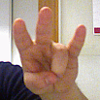
\includegraphics[width=0.15\textwidth]{ChapterFour/1.png}}
    \hfill
    \subfloat{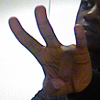
\includegraphics[width=0.15\textwidth]{ChapterFour/4.png}}
    \hfill
    \subfloat{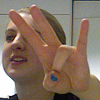
\includegraphics[width=0.15\textwidth]{ChapterFour/3.png}}
    \\\vspace{0.4cm}
    \subfloat{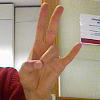
\includegraphics[width=0.15\textwidth]{ChapterFour/2.png}}
    \hfill
    \subfloat{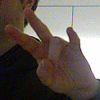
\includegraphics[width=0.15\textwidth]{ChapterFour/5.png}}
    \hfill
    \subfloat{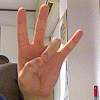
\includegraphics[width=0.15\textwidth]{ChapterFour/6.png}}
    \caption{Inter-signer variability: it is possible to observe not only phonological variations (e.g.\ different handshapes, palm orientations, and sign locations) but also a large physical variability (e.g.\ different hand sizes) when six signers are performing the same sign.}
    \label{fig:inter_signer_variations}
\end{figure}

Borrowing from recent works on adversarial neural networks (\citet{Goodfellow2014, Feutry2018}) and domain transfer (\citet{Ganin2015}), we introduce a deep neural network along with a novel adversarial training objective to specifically tackle the signer-independent SLR problem. The underlying idea is to preserve as much information as possible about the signs, while discarding the signer-specific information that is implicitly present in the manual signing process. For this purpose, the proposed deep model is composed by an \emph{encoder} network, which maps from the input images to latent representations, as well as two discriminative classifiers operating on top of these underlying representations, namely the \emph{sign-classifier} network and the \emph{signer-classifier} network. While the former is trained to predict the sign labels, the latter is trained to identify the signer. In addition, the parameters of the encoder network are optimized to minimize the loss of the sign-classifier while trying to fool the signer-classifier network. This adversarial and competitive training scheme encourages the learned representations to be signer-invariant and highly discriminative for the sign classification task. To further constrain the latent representations to be signer-invariant, we introduce an additional training objective that operates on the hidden representations of the encoder network in order to enforce the latent distributions of different signers to be as similar as possible.

Although this adversarial training framework is similar to those initially introduced by \citet{Ganin2015}, in the context of domain adaptation, and then by \citet{Feutry2018} to learn anonymized representations, our main contributions on top of these works are two-fold: i) the application of the adversarial training concept to the signer-independent SLR problem and ii) a novel adversarial training objective that differs from the ones of \citet{Ganin2015} and \citet{Feutry2018} in two ways. First, our training objective is minimum if and only if the adversarial classifier (i.e.\ the signer-classifier) produces a uniform distribution over the domains (i.e.\ signer identities). Second, we introduce an additional term to the adversarial training objective that further discourages the learned representations of retaining any signer-specific information, by explicitly imposing similarity in the latent distributions of different signers.

The remainder of this section is organized as follows. \Secref{sec:adv_signer_inv_rel_work} presents the related work on SLR. The proposed model along with its adversarial training scheme are fully described in \secref{sec:adv_signer_inv_method}. Experimental results and conclusions are reported in sections~\ref{sec:adv_signer_inv_experiments} and \ref{sec:adv_signer_inv_conclusion}, respectively.

\subsection{Related Work}
\label{sec:adv_signer_inv_rel_work}
We have discussed some of the most relevant approaches for DG in \secref{sec:dg_sota}, so now we shall focus our attention on the specific problem of SLR. This has become an appealing topic in modern society because such systems can ideally be used to reduce the communication barriers that exist between deaf and hearing people.
SLR approaches can be broadly divided into: (i) isolated, which address the recognition of single signs either using static images or video (\citet{Marin2014, Marin2016}), and (ii) continuous, which correspond to the recognition of sentences represented as a sequence of signs (\citet{DanGuo2017, DanGuo2018, Wang2018}). Although most recent works focus on the continuous SLR and its associated problems (e.g.\ large vocabulary size), static SLR is still a challenging task, especially under unconstrained scenarios. One of the biggest challenges is related to the large inter-signer variability, which is in fact the focus of this work.

According to the amount of data required from the test signers, previously signer-independent SLR works can be broadly divided into two main groups: (i) signer adaptation approaches, where a previous trained model is adapted to a new signer by using a small amount of signer specific data, and (ii) truly signer independent methodologies, in which a generic model robust for new test signers is built without using data of those test signers.

The former signer adaptation approaches were greatly inspired by speaker adaptation methods from the speech recognition research. \citet{Agris2006} used maximum likelihood linear regression (MLLR) and maximum a posteriori (MAP) estimation for signer adaptation. In a subsequent work (\citet{Agris2008a}), they extended their work by combining the eigenvoice approach by \citet{Kuhn2000} with MLLR and MAP to adapt trained hidden Markov models (HMMs) to new signers. MLLR and MAP were the basic adaptation strategies, and the eigenvoice approach provided constraints to reduce the number of free parameters to be adapted. More recently, \citet{Kim2016} investigated the potential of several signer normalization techniques (e.g.\ speed normalization) and different deep neural network adaptation strategies for the signer-independence problem. They found that while signer normalization is ineffective, a simple neural network adaptation strategy, such as fine-tuning the signer-specific neural networks on the adaptation data, is very effective.

The aforementioned methods are all supervised adaptation approaches, in the sense that the adaptation data from the new signer must be labeled. However, in practice, collecting labeled data may be a cumbersome and time-consuming task. To overcome this issue, a few works have resorted to unsupervised adaptation strategies. \citet{Yin2015} proposed a two-step weakly supervised metric learning framework to perform signer adaptation with some unlabeled sign data of the new signer. In the first step, a generic metric is learnt from the available labeled data of several different signers. In the second step, the generic metric is adapted to the new signer by considering clustering and manifold constraints along with the collected unlabeled data.

Although signer adaptation is a reasonable approach, there is still the need to collect either labeled or unlabeled data to retrain and adapt the model to a new signer. Therefore, a truly signer-independent approach, which does not require any data from the new signers, would be the ideal solution for a practical SLR system. Examples of such works can be found are those by \citet{Zieren2005, Shanableh2011, Agris2008b, Kong2014, Kelly2010, Dahmani2014, Yin2016}. Most of them involved a huge feature engineering effort in order to build normalized feature descriptors robust to the physical variations of the signers (e.g.\ height, hand size and length of the arm) and different acquisition conditions (e.g.\ distance to the camera). Afterwards, most of these works use HMMs or their variants for sign recognition. It is the example of the work proposed by \citet{Agris2008b}, in which a set of 11 regional features are extracted (e.g.\ 2-D coordinates, hand blobs area, orientation of the main axis, inertia ratio, eccentricity and compactness) and then normalized according to the head position and shoulders distance of the signer. \citet{Kelly2010} introduced a novel signer-independent hand posture feature descriptor, along with an eigenspace size function which represents both qualitative and quantitative properties of a visual shape. \citet{Kong2014} gave particular importance to the movement of epenthesis (ME), which appears as the transition movement that connects successive signs. Concretely speaking, they removed the ME by using a segment and merge approach to decrease the inter-signer variations in ME and used a two-layer conditional random field classifier for sign recognition. More recently, \citet{Yin2016} proposed an interesting and alternative approach that relies on distance metric learning. In particular, the metric is learnt by constraining the distances between the training samples and generic references of the sign classes. The references are constructed by signer invariant representations of each sign class (i.e.\ the average of all samples within the specific class). Afterwards, a two-step iterative optimization strategy is employed to obtain more appropriate references and update the corresponding distance metric alternately.

Although the aforementioned methods have promoted a significant evolution in the signer-independent research, there are still many opportunities for improvement. A major weakness across all the methods is related to the fact that representation and metric learning are not performed jointly. It is well known that the recent success of deep learning approaches, particularly those using CNNs, in tasks like object detection and recognition, has been extended to the SLR problem. The underlying motivation is to automatically learn multiple levels of representations directly from the data (\citet{Pigou2015, Koller2016, Wu2016, Neverova2016, Kumar2017}). However, none of these explicitly constrains the learned representations to be signer invariant.

\section{Methodology}
\label{sec:adv_signer_inv_method}

The ultimate goal of our model is to learn signer-invariant latent representations that preserve the relevant part of the information about the signs while discarding the signer-specific traits that may hamper the sign classification task. To accomplish this purpose, we introduce a deep neural network along with an adversarial training scheme that is able to learn feature representations that combine both sign discriminativeness and signer-invariance.

More specifically, let $\{(\mX_{i},y_{i},s_{i})\}_{i=1}^{n}$ be a labeled dataset of $n$ samples, where $\mX_{i}$ represents the $i$-th colour image, and $y_{i} \in \gY$ and $s_{i} \in \{1,2,\dots,k\}$ denote the corresponding class (sign) label and signer identity, respectively. To induce the model to learn signer-invariant representations, the proposed model comprises three distinct sub-networks:
\begin{itemize}
    \item an encoder network, which aims at learning an encoding function $g(\cdot;\vtheta_g): \gX \mapsto \gZ$, parameterized by $\vtheta_g$, that maps from an input image $\mX \in \gX$ to a latent representation $\vz \in \gZ$;
    \item a sign-classifier network, which operates on top of this underlying latent representation $\vz$ to learn our task-specific function $h(\cdot; \vtheta_h): \gZ \mapsto \gY$, parameterized by $\vtheta_h$, that maps latent vectors into the predicted probabilities of each sign class;
    \item a signer-classifier network, with the purpose of learning a signer-specific function $d(\cdot; \vtheta_d): \gZ \mapsto \{1,2,\dots,k\}$, parameterized by $\vtheta_d$, that maps the same hidden representation $\vz$ into the corresponding signer identity.
\end{itemize}

During the learning stage, the parameters of both classifiers are optimized in order to minimize their errors on their specific tasks on the training set. In addition, the parameters of the encoder network are optimized in order to minimize the loss of the sign-classifier network while forcing the signer-classifier to be a random guessing predictor. In the course of this adversarial training procedure, the learned latent representations $\vz$ are encouraged to be signer-invariant and highly discriminative for sign classification. To further discourage the latent representations of retaining any signer-specific traits, we introduce an additional training objective that enforces the latent distributions of different signers to be as similar as possible.

\subsubsection{Architecture}
As illustrated in \Figref{fig:model_archi}, the architecture of the proposed model is composed by three main sub-networks or blocks, i.e. an encoder, a sign-classifier, and a signer-classifier.

The encoder network attempts to learn a mapping from an input image $\mX$ to a latent representation $\vz$. It consists of a sequence of three pairs of consecutive $3\times 3$ convolutional layers with Rectified  Linear  Units (ReLUs) as non-linearities. For downsampling, the last convolutional layer of each pair has a stride of 2. The number of filters starts as 32 and is doubled after each convolutional pair. The dense layer on top of the encoder network has 128 neurons. On top of that, there is a fully-connected layer, also with a ReLU, outputting the desired signer-invariant latent representations $\vz$.

Taking the latent representations $\vz$ as input, the sign-classifier block is composed by a sequence of three fully-connected layers, with ReLUs as the non-linear functions, for predicting the sign class $\hat{y} \triangleq h(\vz; \vtheta_h)$. The number of nodes of each hidden layer was set to 128. The last fully-connected layer has a softmax activation function which outputs the probabilities for each sign class.

The signer-classifier network has exactly the same topology as the sign-classifier. However, it maps the latent representations $\vz$ to the predicted signer identity $\hat{s} \triangleq d(\vz; \vtheta_d)$. Therefore, the number of nodes of the output layer equals the number of signers in the training set.


\begin{figure*}[t]
\centering
\tikzset{every picture/.style={line width=0.75pt}} %set default line width to 0.75pt

\scalebox{0.6}{










\tikzset{every picture/.style={line width=0.9pt}} %set default line width to 0.75pt

\begin{tikzpicture}[x=0.9pt,y=0.9pt,yscale=-1,xscale=1]
%uncomment if require: \path (0,637); %set diagram left start at 0, and has height of 637

%Shape: Rectangle [id:dp7817430644997849]
\draw  [draw opacity=0][fill={rgb, 255:red, 226; green, 223; blue, 223 }  ,fill opacity=0.46 ][dash pattern={on 4.5pt off 4.5pt}] (89.57,241.83) -- (263.45,241.83) -- (263.45,367) -- (89.57,367) -- cycle ;
%Shape: Rectangle [id:dp43448545781433445]
\draw  [draw opacity=0][fill={rgb, 255:red, 124; green, 163; blue, 233 }  ,fill opacity=0.27 ][dash pattern={on 4.5pt off 4.5pt}] (342,9) -- (521,9) -- (521,93.23) -- (342,93.23) -- cycle ;
%Shape: Rectangle [id:dp47448290384115754]
\draw  [draw opacity=0][fill={rgb, 255:red, 226; green, 223; blue, 223 }  ,fill opacity=0.46 ][dash pattern={on 4.5pt off 4.5pt}] (88.57,60.83) -- (262.45,60.83) -- (262.45,186) -- (88.57,186) -- cycle ;
%Shape: Trapezoid [id:dp7544890433922595]
\draw   (129.83,89.34) -- (166.92,100.47) -- (166.92,161) -- (129.83,172.13) -- cycle ;
%Shape: Rectangle [id:dp07852532899632947]
\draw   (225.83,108) -- (225.83,153.36) -- (210.91,153.36) -- (210.91,108) -- cycle ;
%Straight Lines [id:da6483299081027241]
\draw    (167.27,131.14) -- (208.91,131.24) ;
\draw [shift={(210.91,131.24)}, rotate = 180.14] [fill={rgb, 255:red, 0; green, 0; blue, 0 }  ][line width=0.75]  [draw opacity=0] (8.93,-4.29) -- (0,0) -- (8.93,4.29) -- cycle    ;

%Straight Lines [id:da3383332186453154]
\draw    (64.69,131.46) -- (126.8,131.67) ;
\draw [shift={(128.8,131.68)}, rotate = 180.19] [fill={rgb, 255:red, 0; green, 0; blue, 0 }  ][line width=0.75]  [draw opacity=0] (8.93,-4.29) -- (0,0) -- (8.93,4.29) -- cycle    ;

%Straight Lines [id:da8976159443553993]
\draw    (225.86,131.46) -- (306.79,131.35) ;


%Shape: Rectangle [id:dp39844785350453726]
\draw   (373.93,38.03) -- (373.93,83.38) -- (359.01,83.38) -- (359.01,38.03) -- cycle ;
%Shape: Rectangle [id:dp5960148926786581]
\draw   (412.75,38.03) -- (412.75,83.38) -- (397.84,83.38) -- (397.84,38.03) -- cycle ;
%Shape: Rectangle [id:dp2968748699957451]
\draw   (451.86,45.72) -- (451.86,76.69) -- (436.94,76.69) -- (436.94,45.72) -- cycle ;
%Straight Lines [id:da38135442637321804]
\draw    (374.47,60.94) -- (396.84,60.84) ;
\draw [shift={(398.84,60.83)}, rotate = 539.75] [fill={rgb, 255:red, 0; green, 0; blue, 0 }  ][line width=0.75]  [draw opacity=0] (8.93,-4.29) -- (0,0) -- (8.93,4.29) -- cycle    ;

%Straight Lines [id:da5103446228646831]
\draw    (413.57,60.94) -- (435.94,60.84) ;
\draw [shift={(437.94,60.83)}, rotate = 539.75] [fill={rgb, 255:red, 0; green, 0; blue, 0 }  ][line width=0.75]  [draw opacity=0] (8.93,-4.29) -- (0,0) -- (8.93,4.29) -- cycle    ;

%Shape: Rectangle [id:dp21504155648063916]
\draw  [draw opacity=0][fill={rgb, 255:red, 255; green, 199; blue, 199 }  ,fill opacity=0.46 ][dash pattern={on 4.5pt off 4.5pt}] (342.06,150.9) -- (520.25,150.9) -- (520.25,235.13) -- (342.06,235.13) -- cycle ;
%Shape: Rectangle [id:dp5629086137047858]
\draw   (374.93,179.92) -- (374.93,225.28) -- (360.01,225.28) -- (360.01,179.92) -- cycle ;
%Shape: Rectangle [id:dp11383387176162141]
\draw   (414.75,179.92) -- (414.75,225.28) -- (399.84,225.28) -- (399.84,179.92) -- cycle ;
%Shape: Rectangle [id:dp8834314863600405]
\draw   (453.86,187.61) -- (453.86,218.59) -- (438.94,218.59) -- (438.94,187.61) -- cycle ;
%Straight Lines [id:da7960584409422926]
\draw    (375.47,202.84) -- (397.84,202.74) ;
\draw [shift={(399.84,202.73)}, rotate = 539.75] [fill={rgb, 255:red, 0; green, 0; blue, 0 }  ][line width=0.75]  [draw opacity=0] (8.93,-4.29) -- (0,0) -- (8.93,4.29) -- cycle    ;

%Straight Lines [id:da26603179330471005]
\draw    (414.57,202.84) -- (436.94,202.74) ;
\draw [shift={(438.94,202.73)}, rotate = 539.75] [fill={rgb, 255:red, 0; green, 0; blue, 0 }  ][line width=0.75]  [draw opacity=0] (8.93,-4.29) -- (0,0) -- (8.93,4.29) -- cycle    ;

%Straight Lines [id:da645470302869213]
\draw    (306.79,131.35) -- (307.07,60.72) -- (357,60.99) ;
\draw [shift={(359,61)}, rotate = 180.31] [fill={rgb, 255:red, 0; green, 0; blue, 0 }  ][line width=0.75]  [draw opacity=0] (8.93,-4.29) -- (0,0) -- (8.93,4.29) -- cycle    ;

%Straight Lines [id:da6326177139350364]
\draw    (306.79,131.35) -- (306.74,202.61) -- (357.56,202.5) ;
\draw [shift={(359.56,202.5)}, rotate = 539.88] [fill={rgb, 255:red, 0; green, 0; blue, 0 }  ][line width=0.75]  [draw opacity=0] (8.93,-4.29) -- (0,0) -- (8.93,4.29) -- cycle    ;

%Straight Lines [id:da43094599217232044]
\draw [color={rgb, 255:red, 208; green, 2; blue, 27 }  ,draw opacity=1 ] [dash pattern={on 4.5pt off 4.5pt}]  (452.06,60.88) -- (552.61,60.84) ;
\draw [shift={(554.61,60.83)}, rotate = 539.98] [fill={rgb, 255:red, 208; green, 2; blue, 27 }  ,fill opacity=1 ][line width=0.75]  [draw opacity=0] (8.93,-4.29) -- (0,0) -- (8.93,4.29) -- cycle    ;

%Rounded Rect [id:dp20102262667247417]
\draw  [color={rgb, 255:red, 208; green, 2; blue, 27 }  ,draw opacity=1 ][dash pattern={on 4.5pt off 4.5pt}] (555.16,198.96) .. controls (555.16,197.16) and (556.62,195.71) .. (558.41,195.71) -- (621.75,195.71) .. controls (623.55,195.71) and (625,197.16) .. (625,198.96) -- (625,208.69) .. controls (625,210.48) and (623.55,211.94) .. (621.75,211.94) -- (558.41,211.94) .. controls (556.62,211.94) and (555.16,210.48) .. (555.16,208.69) -- cycle ;
%Straight Lines [id:da7107772326187543]
\draw [color={rgb, 255:red, 208; green, 2; blue, 27 }  ,draw opacity=1 ] [dash pattern={on 4.5pt off 4.5pt}]  (454.25,202.67) -- (552.78,203.37) ;
\draw [shift={(554.78,203.38)}, rotate = 180.41] [fill={rgb, 255:red, 208; green, 2; blue, 27 }  ,fill opacity=1 ][line width=0.75]  [draw opacity=0] (8.93,-4.29) -- (0,0) -- (8.93,4.29) -- cycle    ;

%Straight Lines [id:da7856916848123423]
\draw [color={rgb, 255:red, 208; green, 2; blue, 27 }  ,draw opacity=1 ] [dash pattern={on 4.5pt off 4.5pt}]  (147.5,166.88) -- (147.51,201.24) ;
\draw [shift={(147.51,203.24)}, rotate = 269.99] [fill={rgb, 255:red, 208; green, 2; blue, 27 }  ,fill opacity=1 ][line width=0.75]  [draw opacity=0] (8.93,-4.29) -- (0,0) -- (8.93,4.29) -- cycle    ;

%Straight Lines [id:da899109719860808]
\draw [color={rgb, 255:red, 208; green, 2; blue, 27 }  ,draw opacity=1 ] [dash pattern={on 4.5pt off 4.5pt}]  (217.9,153.87) -- (218.43,202) ;
\draw [shift={(218.45,204)}, rotate = 269.36] [fill={rgb, 255:red, 208; green, 2; blue, 27 }  ,fill opacity=1 ][line width=0.75]  [draw opacity=0] (8.93,-4.29) -- (0,0) -- (8.93,4.29) -- cycle    ;

%Straight Lines [id:da36002582240035363]
\draw [color={rgb, 255:red, 0; green, 0; blue, 0 }  ,draw opacity=1 ][line width=0.75]    (186.6,226.85) .. controls (188.27,228.52) and (188.27,230.18) .. (186.6,231.85) .. controls (184.93,233.52) and (184.93,235.18) .. (186.6,236.85) -- (186.6,239.85) -- (186.6,239.85)(183.6,226.85) .. controls (185.27,228.52) and (185.27,230.18) .. (183.6,231.85) .. controls (181.93,233.52) and (181.93,235.18) .. (183.6,236.85) -- (183.6,239.85) -- (183.6,239.85) ;


%Rounded Rect [id:dp28118263286951617]
\draw  [color={rgb, 255:red, 208; green, 2; blue, 27 }  ,draw opacity=1 ][dash pattern={on 4.5pt off 4.5pt}] (556.16,55.96) .. controls (556.16,54.16) and (557.62,52.71) .. (559.41,52.71) -- (622.75,52.71) .. controls (624.55,52.71) and (626,54.16) .. (626,55.96) -- (626,65.69) .. controls (626,67.48) and (624.55,68.94) .. (622.75,68.94) -- (559.41,68.94) .. controls (557.62,68.94) and (556.16,67.48) .. (556.16,65.69) -- cycle ;
%Straight Lines [id:da5356763271282314]
\draw [color={rgb, 255:red, 208; green, 2; blue, 27 }  ,draw opacity=1 ] [dash pattern={on 4.5pt off 4.5pt}]  (591.52,72.62) -- (591.71,101.6) ;

\draw [shift={(591.51,70.62)}, rotate = 89.63] [fill={rgb, 255:red, 208; green, 2; blue, 27 }  ,fill opacity=1 ][line width=0.75]  [draw opacity=0] (8.93,-4.29) -- (0,0) -- (8.93,4.29) -- cycle    ;
%Straight Lines [id:da9155638065763507]
\draw [color={rgb, 255:red, 208; green, 2; blue, 27 }  ,draw opacity=1 ] [dash pattern={on 4.5pt off 4.5pt}]  (590.12,215.42) -- (590.31,244.4) ;

\draw [shift={(590.11,213.42)}, rotate = 89.63] [fill={rgb, 255:red, 208; green, 2; blue, 27 }  ,fill opacity=1 ][line width=0.75]  [draw opacity=0] (8.93,-4.29) -- (0,0) -- (8.93,4.29) -- cycle    ;
%Straight Lines [id:da7191094178180941]
\draw [color={rgb, 255:red, 0; green, 0; blue, 0 }  ,draw opacity=1 ][line width=0.75]    (186.6,187.85) .. controls (188.27,189.52) and (188.27,191.18) .. (186.6,192.85) .. controls (184.93,194.52) and (184.93,196.18) .. (186.6,197.85) -- (186.6,200.85) -- (186.6,200.85)(183.6,187.85) .. controls (185.27,189.52) and (185.27,191.18) .. (183.6,192.85) .. controls (181.93,194.52) and (181.93,196.18) .. (183.6,197.85) -- (183.6,200.85) -- (183.6,200.85) ;


%Straight Lines [id:da9896530377071313]
\draw [color={rgb, 255:red, 208; green, 2; blue, 27 }  ,draw opacity=1 ] [dash pattern={on 4.5pt off 4.5pt}]  (147.51,226.56) -- (147.5,259.88) ;

\draw [shift={(147.51,224.56)}, rotate = 90.02] [fill={rgb, 255:red, 208; green, 2; blue, 27 }  ,fill opacity=1 ][line width=0.75]  [draw opacity=0] (8.93,-4.29) -- (0,0) -- (8.93,4.29) -- cycle    ;
%Shape: Trapezoid [id:dp6458709768563871]
\draw   (672,269.5) -- (683,272.8) -- (683,304.2) -- (672,307.5) -- cycle ;
%Shape: Rectangle [id:dp1901046474760686]
\draw   (226.83,273) -- (226.83,318.36) -- (211.91,318.36) -- (211.91,273) -- cycle ;
%Straight Lines [id:da8673211689855849]
\draw    (168.27,296.14) -- (209.91,296.24) ;
\draw [shift={(211.91,296.24)}, rotate = 180.14] [fill={rgb, 255:red, 0; green, 0; blue, 0 }  ][line width=0.75]  [draw opacity=0] (8.93,-4.29) -- (0,0) -- (8.93,4.29) -- cycle    ;

%Straight Lines [id:da3618642920648949]
\draw    (65.69,296.46) -- (127.8,296.67) ;
\draw [shift={(129.8,296.68)}, rotate = 180.19] [fill={rgb, 255:red, 0; green, 0; blue, 0 }  ][line width=0.75]  [draw opacity=0] (8.93,-4.29) -- (0,0) -- (8.93,4.29) -- cycle    ;

%Rounded Rect [id:dp5531536926433998]
\draw  [color={rgb, 255:red, 208; green, 2; blue, 27 }  ,draw opacity=1 ][dash pattern={on 4.5pt off 4.5pt}] (129.28,207.86) .. controls (129.28,205.77) and (130.98,204.07) .. (133.07,204.07) -- (231.08,204.07) .. controls (233.17,204.07) and (234.86,205.77) .. (234.86,207.86) -- (234.86,219.21) .. controls (234.86,221.31) and (233.17,223) .. (231.08,223) -- (133.07,223) .. controls (130.98,223) and (129.28,221.31) .. (129.28,219.21) -- cycle ;
%Straight Lines [id:da5399866438305847]
\draw [color={rgb, 255:red, 208; green, 2; blue, 27 }  ,draw opacity=1 ] [dash pattern={on 4.5pt off 4.5pt}]  (218.58,225.21) -- (219.12,273.33) ;

\draw [shift={(218.56,223.21)}, rotate = 89.36] [fill={rgb, 255:red, 208; green, 2; blue, 27 }  ,fill opacity=1 ][line width=0.75]  [draw opacity=0] (8.93,-4.29) -- (0,0) -- (8.93,4.29) -- cycle    ;
%Straight Lines [id:da6744189660599909]
\draw [color={rgb, 255:red, 208; green, 2; blue, 27 }  ,draw opacity=1 ] [dash pattern={on 4.5pt off 4.5pt}]  (532.07,202.88) -- (532.47,295.68) -- (552.87,295.68) ;
\draw [shift={(554.87,295.68)}, rotate = 180] [fill={rgb, 255:red, 208; green, 2; blue, 27 }  ,fill opacity=1 ][line width=0.75]  [draw opacity=0] (8.93,-4.29) -- (0,0) -- (8.93,4.29) -- cycle    ;
\draw [shift={(532.07,202.88)}, rotate = 89.75] [color={rgb, 255:red, 208; green, 2; blue, 27 }  ,draw opacity=1 ][fill={rgb, 255:red, 208; green, 2; blue, 27 }  ,fill opacity=1 ][line width=0.75]      (0, 0) circle [x radius= 3.35, y radius= 3.35]   ;
%Rounded Rect [id:dp27586876312894315]
\draw  [color={rgb, 255:red, 208; green, 2; blue, 27 }  ,draw opacity=1 ][dash pattern={on 4.5pt off 4.5pt}] (554.76,291.36) .. controls (554.76,289.56) and (556.22,288.11) .. (558.01,288.11) -- (621.35,288.11) .. controls (623.15,288.11) and (624.6,289.56) .. (624.6,291.36) -- (624.6,301.09) .. controls (624.6,302.88) and (623.15,304.34) .. (621.35,304.34) -- (558.01,304.34) .. controls (556.22,304.34) and (554.76,302.88) .. (554.76,301.09) -- cycle ;
%Straight Lines [id:da05722319267703546]
\draw [color={rgb, 255:red, 208; green, 2; blue, 27 }  ,draw opacity=1 ] [dash pattern={on 4.5pt off 4.5pt}]  (590.37,307.67) -- (590.56,336.65) ;

\draw [shift={(590.36,305.67)}, rotate = 89.63] [fill={rgb, 255:red, 208; green, 2; blue, 27 }  ,fill opacity=1 ][line width=0.75]  [draw opacity=0] (8.93,-4.29) -- (0,0) -- (8.93,4.29) -- cycle    ;
%Shape: Trapezoid [id:dp41106407745048745]
\draw   (130.83,255.34) -- (167.92,266.47) -- (167.92,327) -- (130.83,338.13) -- cycle ;
%Shape: Rectangle [id:dp5258454923666749]
\draw   (683,319) -- (683,353) -- (671.91,353) -- (671.91,319) -- cycle ;

% Text Node
\draw (46.68,132.11) node   {$\boldsymbol{X}_{i}$};
% Text Node
\draw (48.35,213.89) node  [align=left] {\textbf{{\large .}}\\\textbf{{\large .}}\\\textbf{{\large .}}};
% Text Node
\draw (145.74,72.5) node  [align=left] {{\small \textit{Encoder network:}}};
% Text Node
\draw (215.7,74.44) node   {$h(\boldsymbol{X}\mathrm{;}\mathnormal{\theta _{h}})$};
% Text Node
\draw (387.48,20.66) node  [align=left] {{\small \textit{Sign-classifier:}}};
% Text Node
\draw (448.89,20.95) node   {$f(\boldsymbol{z}\mathrm{;}\mathnormal{\theta _{f}})$};
% Text Node
\draw (393.24,162.34) node  [align=left] {{\small \textit{Signer-classifier:}}};
% Text Node
\draw (456.63,161.64) node   {$g(\boldsymbol{z}\mathrm{;}\mathnormal{\theta _{g}})$};
% Text Node
\draw (589.25,204.03) node   {${\textstyle \mathcal{\textcolor[rgb]{0.82,0.01,0.11}{L}}\textcolor[rgb]{0.82,0.01,0.11}{_{\mathrm{signer}}}}$};
% Text Node
\draw (489.39,48.2) node   {$p( y_{i} |\boldsymbol{z}_{i} ;\mathnormal{\theta _{f}})$};
% Text Node
\draw (247.56,124.01) node   {$\boldsymbol{z}_{i}$};
% Text Node
\draw (179.66,212.92) node   {${\textstyle \mathcal{\textcolor[rgb]{0.82,0.01,0.11}{L}}\textcolor[rgb]{0.82,0.01,0.11}{_{\mathrm{transfer}}}}$};
% Text Node
\draw (590.25,61.03) node   {${\textstyle \mathcal{\textcolor[rgb]{0.82,0.01,0.11}{L}}\textcolor[rgb]{0.82,0.01,0.11}{_{\mathrm{sign}}}}$};
% Text Node
\draw (593,110.17) node   {$y_{i}$};
% Text Node
\draw (591.6,252.97) node   {$s_{i}$};
% Text Node
\draw (47.68,297.11) node   {$\boldsymbol{X}_{j}$};
% Text Node
\draw (145.74,355.5) node  [align=left] {{\small \textit{Encoder network:}}};
% Text Node
\draw (215.7,357.44) node   {$h(\mathbf{X}\mathrm{;}\mathnormal{\theta _{h}})$};
% Text Node
\draw (588.85,295.43) node   {${\textstyle \mathcal{\textcolor[rgb]{0.82,0.01,0.11}{L}}\textcolor[rgb]{0.82,0.01,0.11}{_{\mathrm{adv}}}}$};
% Text Node
\draw (591.85,345.22) node   {$\mathcal{U}(\mathrm{s})$};
% Text Node
\draw (755,289) node  [align=left] {{\scriptsize Block of convolutional layers}};
% Text Node
\draw (738,335.5) node  [align=left] {{\scriptsize Fully-connected layer}};
% Text Node
\draw (53.96,327) node [scale=0.9]  {$\mathnormal{s_{j} \neq s_{i}}$};
% Text Node
\draw (489.89,190.7) node   {$p( s_{i} |\boldsymbol{z}_{i} ;\mathnormal{\theta _{g}})$};


\end{tikzpicture}




}

\caption{The architecture of the proposed signer-invariant neural network. It comprises three main sub-networks or blocks, i.e. an \textit{encoder}, a \textit{sign-classifier} and a \textit{signer-classifier}.}
\label{fig:model_archi}
\end{figure*}


\subsubsection{Adversarial training}
By definition, signer-invariant representations discard all signer-specific information and, as such, no function (i.e.\ classifier) exists that maps such representations into the correct signer identity. This naturally leads to an adversarial problem, in which: (i) a signer-classifier network $d(\cdot; \vtheta_d)$ receives latent representations $\vz \triangleq g(\mX;\vtheta_g)$ from an encoder network $g(\cdot;\vtheta_g)$ and tries to predict the signer identity $s$ corresponding to image $\mX$ and (ii) the encoder network tries to fool the signer-classifier network while still providing good representations for the sign-classifier network $h(\cdot; \vtheta_h)$, which in turn receives the same representations $\vz$ and aims to predict the sign label $y$ corresponding to image $\mX$.

Therefore, the signer-classifier network shall be trained to minimize the negative log-likelihood of correct signer predictions:
\begin{equation}
\label{eq:signer_loss}
\min_{\vtheta_d} \; \left\lbrace L_{\text{signer}}(\vtheta_g, \vtheta_d) \triangleq -\frac{1}{n}\sum_{i=1}^n \log p(s_i \mid g(\mX_{i}; \vtheta_g); \theta_d) \right\rbrace
\end{equation}

In the perspective of the encoder, the predictions of the sign-classifier should be as accurate as possible and the predictions of the signer-classifier should be kept close to uniform, meaning that this latter model is not capable of doing better than random guessing the signer identity. Formally, this may be translated into the following constrained objective:
\begin{align}
\label{eq:sign_loss}
&\min_{\vtheta_g, \vtheta_h} \; \left\lbrace L_{\text{sign}}(\vtheta_g, \vtheta_h)\triangleq-\frac{1}{n}\sum_{i=1}^n \log p(y_i \mid g(\mX_{i}; \vtheta_g); \vtheta_h)\right\rbrace,\\
\label{eq:kl_obj}
&\text{subject to } \; \frac{1}{n}\sum_{i=1}^n \KL(\gU(\rs) || p(\rs \mid g(\mX_{i}; \vtheta_h); \vtheta_g) \leq \epsilon,
\end{align}
where $\KL$ is the Kullback-Leibler (KL) divergence and $\gU(\rs)$ denotes the discrete uniform distribution on the random variable $\rs$, defined over the set of signer identities $\{1, 2, \dots, k\}$ in the training set. Here, $\epsilon \geq 0$ determines how far from uniform the signer-classifier predictions are allowed to be (as measured by the KL divergence). The choice of the uniform distribution implies the underlying assumption that the training set is balanced relatively to the number of examples per signer (which should be true for most practical datasets). When this is not the case, the empirical distribution of signer identities in the training set may be used instead.

The inequality constraint~\plaineqref{eq:kl_obj} may be rewritten as:
\begin{equation}
\label{eq:adv_loss}
L_{\text{adv}}(\vtheta_g, \vtheta_d) \triangleq \frac{1}{nk}\sum_{i=1}^n \sum_{\rs} \log p(\rs \mid g(\mX_{i}; \vtheta_g); \vtheta_d) \leq \epsilon + \log k,
\end{equation}
and the constrained optimization problem may be equivalently formulated as:
\begin{equation}
\label{eq:tr_obj}
\min_{\vtheta_g, \vtheta_h}  \left\lbrace L(\vtheta_g, \vtheta_h, \vtheta_d) \triangleq L_{\text{sign}}(\vtheta_g, \vtheta_h) + \mu_d L_{\text{adv}}(\vtheta_g, \vtheta_d) \right\rbrace,
\end{equation}
where $\mu_d \geq 0$ depends on $\epsilon$ and $L_{\text{adv}}$ plays the role of an adversarial loss with respect to the signer classification loss $L_{\text{signer}}$.

This objective and the structure of our model are similar to those used by \citet{Ganin2015}, in the context of domain adaptation, and by \citet{Feutry2018}, to learn anonymized representations for privacy purposes. However, the former uses the negative signer classification loss as the adversarial term (i.e.\ $L_{\text{adv}} \leftarrow -L_{\text{signer}}$), which is not lower bounded, leading to high gradients and more difficult optimization. The latter addresses this problem by replacing this term with the absolute difference between the adversarial loss as defined in \eqref{eq:adv_loss} and the signer classification loss (i.e.\ $L_{\text{adv}} \leftarrow |L_{\text{adv}} - L_{\text{signer}}|$). This option has a nice information theoretic interpretation as being an empirical upper-bound for the mutual information between the distribution of signer identities and the distribution of latent representations. Nonetheless, there exist infinitely many (non-uniform) distributions for which this loss vanishes. Our choice, besides being clearly lower bounded by the entropy of the uniform distribution, $\log k$, is minimum if and only if $p(\rs \mid g(\mX_{i}; \vtheta_g); \vtheta_d) \equiv \gU(\rs)$, $\forall i$, meaning that the signer-classifier block is completely agnostic relatively to the signer identities of the training samples.

\subsubsection{Signer-transfer training objective}
To further encourage the latent representations $\vz$ to be signer-invariant, we introduce an additional term in objective~\plaineqref{eq:tr_obj}, the so-called signer-transfer loss $L_{\text{transfer}}$. The core idea of $L_{\text{transfer}}$ is to match first order statistics of different signers earlier in the network. For this purpose, let $g^{(l)}(\cdot;\vtheta_g)$ be the $l$-th layer of the encoder network, $l \in \{1,...,m\}$, and consider the distance $\gD^{(l)}(s, s'; \vtheta_g)$ between two distinct signers $s$ and $s'$, defined as:
\begin{equation}
\label{eq:sign_transfer_pairwise_loss}
\gD^{(l)}(s, s'; \vtheta_g) \triangleq \Big|\Big| \frac{1}{n_s} \sum_{i=1}^n g^{(l)}(\mX_{i}; \vtheta_g) \1_{s_i = s} - \frac{1}{n_{s'}}\sum_{j=1}^n g^{(l)}(\mX_{j}; \vtheta_g) \1_{s_j = s'} \Big|\Big|_2^2,
\end{equation}
where $||\bcdot||_2$ is the $\normltwo$-norm, and $n_s$ and $n_{s'}$ denote the number of training examples for signers $s$ and $s'$, respectively. Accordingly, the signer-transfer loss at the $l$-th layer is the sum of the pairwise distances between all signers, i.e.:
\begin{equation}
L_{\text{transfer}}^{(l)}(\vtheta_g) \triangleq \sum_{\substack{s,s'=1 \\ s' \neq s}}^k \gD^{(l)}(s,s'; \vtheta_g).
\end{equation}
The overall signer-transfer loss $L_{\text{transfer}}$ is then a weighted sum of the losses computed at each layer of the encoder network:
\begin{equation}
\label{eq:signer_transfer_loss}
L_{\text{transfer}}(\vtheta_g) \triangleq \sum_{l=1}^{m} \beta^{(l)} L_{\text{transfer}}^{(l)}(\vtheta_g),
\end{equation}
where $\beta^{(l)}\geq 0$ is a hyperparameter that controls the relative importance of the loss obtained at the $l$-th layer.
By combining \plaineqref{eq:tr_obj} and \plaineqref{eq:signer_transfer_loss}, the encoder and sign-classifier networks are trained to minimize the following loss function:
\begin{equation}
\label{eq:enc_sign_loss}
\min_{\vtheta_g, \vtheta_h} \left\lbrace L(\vtheta_g, \vtheta_h, \vtheta_d) \triangleq L_{\text{sign}}(\vtheta_g, \vtheta_h) + \mu_d L_{\text{adv}}(\vtheta_g, \vtheta_d) +
\mu_t L_{\text{transfer}}(\vtheta_g) \right\rbrace,
\end{equation}
where $\mu_t \geq 0$ is the weight that controls the relative importance of the signer-transfer term.

Summing up, the adversarial training procedure is organized by alternating between the minimization of objective~\plaineqref{eq:enc_sign_loss} and the minimization of objective~\plaineqref{eq:signer_loss}.

\subsection{Experiments}
\label{sec:adv_signer_inv_experiments}

\subsubsection{Datasets}
The experimental evaluation of the proposed model was performed using two publicly available SLR databases: the Jochen-Triesch database (\citet{Triesch2001}) and the Microsoft Kinect and Leap Motion American sign language (MKLM) database (\citet{Marin2014, Marin2016}).

Jochen-Triesch is a static hand posture database, which consists of 10 hand posture signs performed by a total of 24 subjects against three types of backgrounds: uniform light, uniform dark and complex (see \Figref{fig:jochen_triesch}). There exist three images for each subject and sign, one for each background type. The images of the Jochen-Triesch database are in grey-scale with a resolution of $128\times 128$ pixels. Experiments on the Jochen-Triesch dataset were conducted using an available standard evaluation protocol for this dataset \cite{Just_2006}, in which 8 subjects are used for the training and the remaining 16 subjects are used for testing. For tuning the hyperparameters of the models, the training set is further divided, also with signer independence, in $80\%$ for training and $20\%$ for validation.

MKLM is a balanced dataset of 10 classes, representing 10 static gestures from the American sign language (see \Figref{fig:mklm}). Each sign was performed by 14 different people, and repeated 10 times, which results in a total of 1400 gestures. Contrary to the Jochen-Triesch database, there is no standard evaluation protocol for the MKLM database. To maximize the usage of the data in the evaluation process, the performance of the models was assessed using a five-fold cross validation scheme with signer independence. This evaluation scheme yields at each split a training set composed by 10 signers, a validation set of 2 signers and a test set with the remaining 2 signers.

In order to extract the manual signs from the noisy background of the images, the automatic hand detection algorithm (\citet{Ferreira2018}) is used as a pre-processing step. The images are then cropped, resized to the average sign size of the training set, and normalized to be in the range $[-1,1]$.

\begin{figure}[t]
    \centering
    \def\altura{0.065}
    \begin{subfigure}{0.45\textwidth}
        \centering
        \setlength{\fboxsep}{0pt}
        \fbox{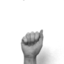
\includegraphics[height=\altura\textheight, keepaspectratio]{ChapterFour/triesch_1.png}}
        \fbox{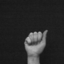
\includegraphics[height=\altura\textheight, keepaspectratio]{ChapterFour/triesch_2.png}}
        \fbox{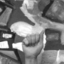
\includegraphics[height=\altura\textheight, keepaspectratio]{ChapterFour/triesch_3.png}} \\\vspace{3px}
        \fbox{
\includegraphics[height=\altura\textheight, keepaspectratio]{ChapterFour/triesch_4.png}}
        \fbox{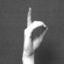
\includegraphics[height=\altura\textheight, keepaspectratio]{ChapterFour/triesch_5.png}}
        \fbox{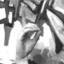
\includegraphics[height=\altura\textheight, keepaspectratio]{ChapterFour/triesch_6.png}} \\\vspace{3px}
        \fbox{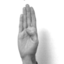
\includegraphics[height=\altura\textheight, keepaspectratio]{ChapterFour/triesch_7.png}}
        \fbox{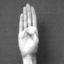
\includegraphics[height=\altura\textheight, keepaspectratio]{ChapterFour/triesch_8.png}}
        \fbox{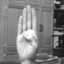
\includegraphics[height=\altura\textheight, keepaspectratio]{ChapterFour/triesch_9.png}}
        \caption{Jochen-Triesch}
        \label{fig:jochen_triesch}
    \end{subfigure}
    \quad
    \begin{subfigure}{0.45\textwidth}
        \centering
        \setlength{\fboxsep}{0pt}
        \fbox{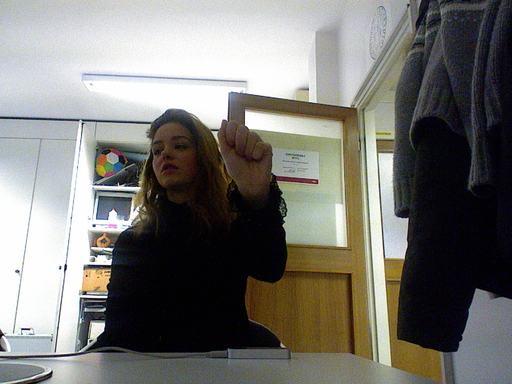
\includegraphics[height=\altura\textheight, keepaspectratio]{ChapterFour/MKLM_1.png}}
        \fbox{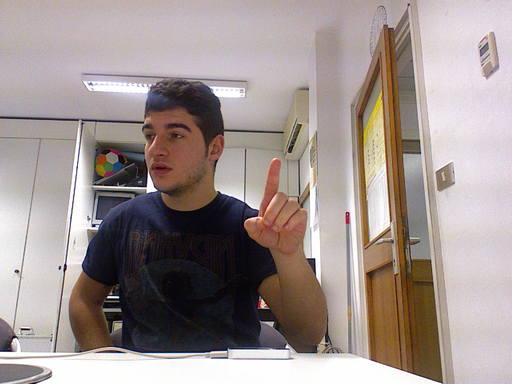
\includegraphics[height=\altura\textheight, keepaspectratio]{ChapterFour/MKLM_2.png}}
        \fbox{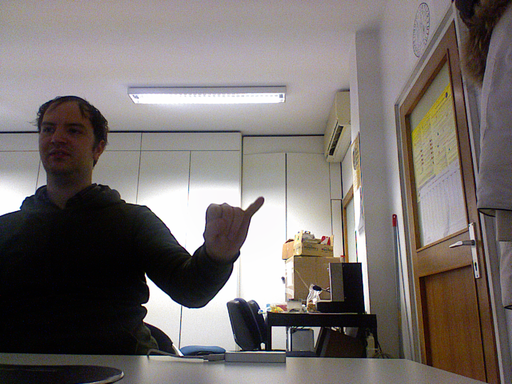
\includegraphics[height=\altura\textheight, keepaspectratio]{ChapterFour/MKLM_3.png}} \\\vspace{3px}
        \fbox{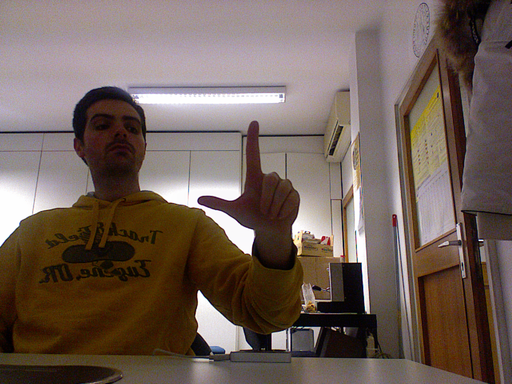
\includegraphics[height=\altura\textheight, keepaspectratio]{ChapterFour/MKLM_4.png}}
        \fbox{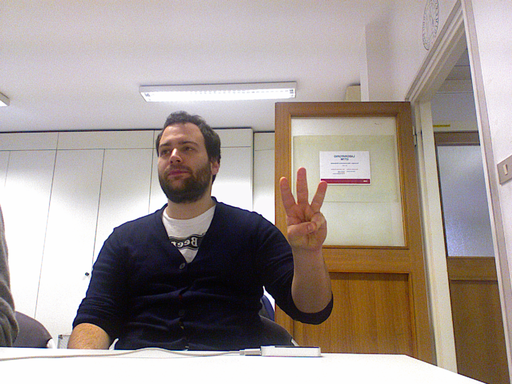
\includegraphics[height=\altura\textheight, keepaspectratio]{ChapterFour/MKLM_6.png}}
        \fbox{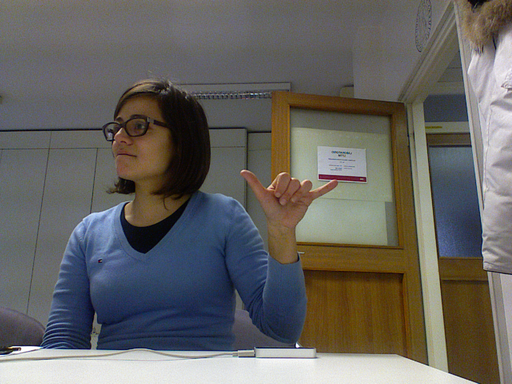
\includegraphics[height=\altura\textheight, keepaspectratio]{ChapterFour/MKLM_7.png}} \\\vspace{3px}
        \fbox{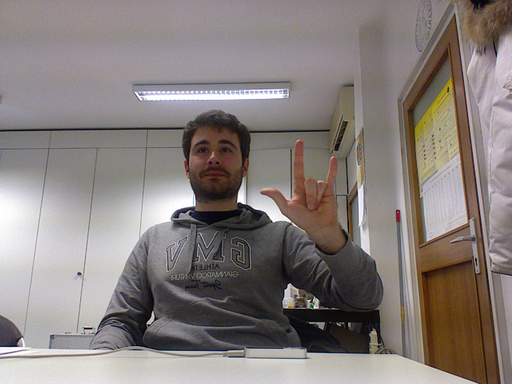
\includegraphics[height=\altura\textheight, keepaspectratio]{ChapterFour/MKLM_8.png}}
        \fbox{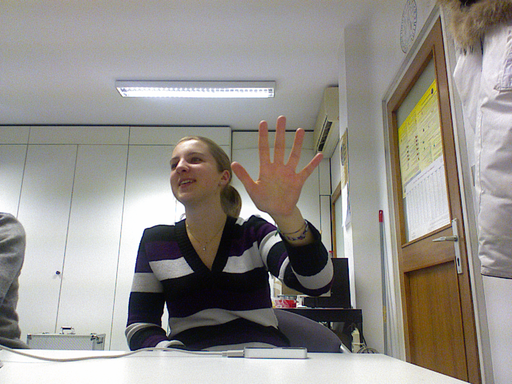
\includegraphics[height=\altura\textheight, keepaspectratio]{ChapterFour/MKLM_9.png}}
        \fbox{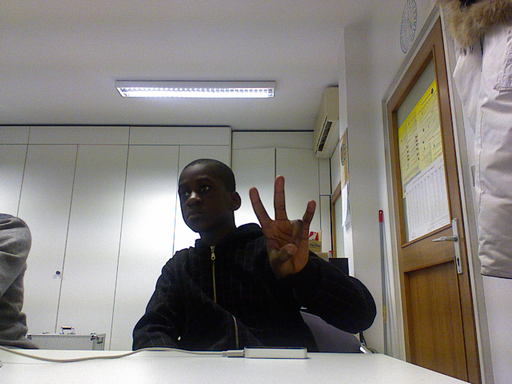
\includegraphics[height=\altura\textheight, keepaspectratio]{ChapterFour/MKLM_10.png}}
        \caption{MKLM}
        \label{fig:mklm}
    \end{subfigure}
    \caption{Illustrative samples of the two datasets used in the experiments.}
    \label{fig:datasets}
\end{figure}

\subsubsection{Baselines}
Throughout this section, the proposed model is compared with state of the art methods for each dataset. Nevertheless, to further attest the robustness of the proposed model, two different baselines are also implemented:
\begin{itemize}
    \item (Baseline 1) A CNN trained from scratch with $\normltwo$ regularization. For a fair comparison, the architecture of the baseline CNN corresponds to the architecture of the encoder network followed by the sign-classifier network of the proposed model.
    \item (Baseline 2) A CNN with the baseline 1 topology, but trained with the triplet loss (\citet{Schroff2015}).
\end{itemize}
Here, the triplet loss concept is explored in order to impose signer-independence in the representation space and, hence, build up a more robust baseline. The underlying idea is to minimize the distance between an \textit{anchor} and a \textit{positive} latent representation, $\vz_{y_{i}, s_{i}}$ and $\vz_{y_{p}, s_{p}}$, respectively; while maximizing the distance between the anchor $\vz_{y_{i}, s_{i}}$ and a \textit{negative} representation $\vz_{y_{n}, s_{n}}$. It is important to note that while anchor and positive latent representations have to be from the same sign class, their signer identity may or not change. On the other hand, anchor and negative representations are from different sign classes, whereas their signer identity may also change. In order to train baseline 2 in an end-to-end fashion for sign classification, the overall loss function to be minimized is a trade-off between the triplet loss $L_{\text{triplet}}$, defined below, and the classification loss $L_{\text{sign}}$:
\begin{equation}
L_{\text{triplet}} \triangleq \frac{1}{n}\sum_{i=1}^{n}\Big[||\vz_{y_{i}, s_{i}}-\vz_{y_{p}, s_{p}}||^2_2 - ||\vz_{y_{i}, s_{i}}-\vz_{y_{n}, s_{n}}||^2_2 + \alpha\Big],
\end{equation}
where $y_{p}=y_{i}$ and $y_{n} \neq y_{i}$ and the margin $\alpha$ enforced between \emph{positive} and \emph{negative} pairs was fixed at $\alpha=1$. In addition, following \citet{Schroff2015}, we adopted an \emph{online} triplet generation strategy, by selecting the hardest positive/negative samples within every mini-batch. The overall loss for this model is therefore $L_{\text{sign}} + \rho L_{\text{triplet}}$, where $\rho \geq 0$ is a hyperparameter.

All deep models were implemented in PyTorch and trained with the Adam optimization algorithm using a batch size of 32 samples. For reproducibility purposes, the source code as well as the weights of the trained models are publicly available online\footnote{\url{https://github.com/pmmf/SI-SLR}}. The hyperparameters that are common to all the implemented models (i.e.\ learning rate and $\normltwo$ regularization weight) as well as some hyperparameters that are specific to the proposed model (i.e.\ $\mu_d$ and $\mu_t$) and to the implemented baseline~2 (i.e.\ $\rho$) were optimized by means of a grid search approach and cross-validation on the training set (see \Tableref{tab:hyperparam} for more details). The signer-transfer penalty $L_{\text{transfer}}$ is applied to the last two layers of the encoder network with a relative weight of 1.

\begin{table}[t]
    \centering
        \begin{tabular}{c|c|c}
            Hyperparameters                    & Symbol & Set                \\ \hline
            Leaning rate                                & --      & \{$1\text{e}^{-04}$,$1\text{e}^{-03}$\}             \\
            $\normltwo$-norm coefficient                              & --       & \{$1\text{e}^{-05}$,$1\text{e}^{-04}$\}             \\
            $L_{\text{triplet}}$ weight                 & $\rho$                & \{0.1,0.5,1,5,10\}                  \\
            $L_{\text{adv}}$ weight                 & $\mu_d$                & \{0.1,0.5,0.8,1,3\}                  \\
            $L_{\text{transfer}}$ weight                 & $\mu_t$                & $\{1.5\text{e}^{-04}$,$2\text{e}^{-04}$,$4\text{e}^{-04}$,$1\text{e}^{-03}\}$
        \end{tabular}
    \caption{Hyperparameter sets for the proposed adversarial model and baselines.}
    \label{tab:hyperparam}
\end{table}

\subsubsection{Results and discussion}
Experiments on the Jochen-Triesch and MKLM databases are summarized in \Tableref{tab:adv_signer_inv_results}. We compare our method with other state of the art approaches that have published results on these datasets (\citet{Dahmani2014, Just2006, Kelly2010, Marin2014, Ferreira2018}). The results on the Jochen-Triesch database are presented in terms of average classification accuracy in the overall test set as well as against each specific background type (i.e.\ uniform and complex). For the MKLM database, the table shows the average classification accuracy computed across all test splits, as well as the minimum and maximum accuracy value achieved by each method.

\begin{table}[t]
    \centering
    \resizebox{\linewidth}{!}{
    \begin{tabular}{c|c c c|c c c}
                & \multicolumn{3}{c|}{Jochen Triesch} & \multicolumn{3}{c}{MKLM}\\
                & Uniform  Bg.      & Complex Bg.        & Both  & Avg. $\pm$ std.  & min         & max        \\ \hline
                \citet{Just2006}       & 92.79           & 81.25           & 87.92         & -- & -- & --\\
                \citet{Kelly2010} & 91.80 & -- & -- & -- & -- & --\\
                \citet{Dahmani2014} & 93.10 & -- & -- & -- & -- & --\\
                \citet{Marin2014}  & -- & --  & -- & 89.71 & -- & --\\
                \citet{Ferreira2018} & -- & --  & -- & 93.17 & -- & -- \\
                \hline
                CNN (baseline 1)                            & 97.50           & 74.38           & 89.79   & 89.90 \footnotesize{$\pm 8.81$}            & 73.00                & 98.00\\
                CNN with triplet loss (baseline 2)          & 98.13           & 75.63           & 90.63 & 91.40 \footnotesize{$\pm 3.93$}             & 86.50                & 96.50\\
                Proposed method       &      \textbf{98.75}     & \textbf{ 91.25}
                &   \textbf{96.25} &    \textbf{94.80} \footnotesize{$\pm 3.53$}      &   \textbf{89.50}
                &  \textbf{100.00}
    \end{tabular}}
    \caption{Classification accuracy (\%) of the proposed adversarial method and baselines on Jochen-Triesch and MKLM datasets.}
    \label{tab:adv_signer_inv_results}
\end{table}

The most relevant observation is the superior performance of the proposed model. Specifically, the proposed model provides the best overall classification accuracy on both SLR databases, clearly outperforming both implemented baselines and all the previous state of the art models. In Jochen-Triesch, the most challenging data are the images with complex background, where the proposed model surpasses all the remaining by a large margin. In addition, by analyzing the standard deviation as well as the minimum and maximum accuracy values, it is possible to observe that the proposed model is the method with the lowest variability, yielding consistently high accuracy rates across all test splits of the MKLM dataset. These results attest the robustness of the proposed model and its capability of better dealing with the large inter-signer variability that exists in the manual signing process of sign languages. Interestingly, the obtained results also reveal that the implemented baselines are in fact fairly strong models, both of them outperforming most of the state of the art methods on both datasets.

\Tableref{tab:loss_terms} illustrates the effect of each proposed training scheme by itself. For this purpose, the proposed model was trained either (i) with just the adversarial procedure, without the signer-transfer $L_{\text{transfer}}$ loss, or (ii) with just the $L_{\text{transfer}}$ penalty on the encoder network without adversarial training. The results clearly demonstrate the complementary effect between the two training procedures, as their combination provides the best overall classification accuracy. Interestingly, each training scheme outperforms on its own both baselines and state of the art methods.

\begin{table}[t]
    \centering
    \begin{small}
        \begin{tabular}{c|c c : c }
            & Adversarial ($L_{\text{adv}}$) only  & Signer-transfer ($L_{\text{transfer}}$) only & Both \\ \hline
            Jochen-Triesch                              & 95.21            & 94.38                & \textbf{96.25}        \\
            MKLM            & 94.00            & 94.10                & \textbf{94.80}
        \end{tabular}
    \end{small}
    \caption{\centering The effect of each training procedure in the proposed model. The results in the last column are replicated from \Tableref{tab:joint_table} as they include both training procedures.}
    \label{tab:loss_terms}
\end{table}

\subsubsection{Latent space visualization}
\label{sec:adv_signer_inv_tsne}
To further demonstrate the effectiveness of the proposed model in promoting signer-invariant latent representation spaces, we show in \Figref{fig:adv_signer_inv_tsne} a visual inspection of the latent representations through the t-distributed stochastic neighbor embedding (t-SNE, \citet{Maaten2008}). These plots clearly demonstrate the better capability of the proposed model of imposing signer-independence in the latent representations. The proposed model yields a latent representation space in which representations of different signers and same class are close to each other and well mixed, while it keeps latent representations of different classes far apart. By analyzing the t-SNE plot of baseline 1, it is possible to observe that the latent representations of different signers and the same class tend to be far apart in the latent space. In addition, there is some overlapping between clusters of different classes. Although baseline 2 (CNN with the triplet loss) promoted slightly improvements over the standard baseline CNN, the proposed model achieved by far the best signer-invariance and class separability.

\begin{figure}
    \centering
    \begin{subfigure}[t]{0.32\textwidth}
        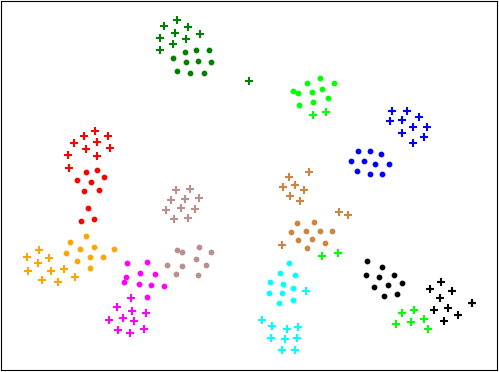
\includegraphics[width=\textwidth]{ChapterFour/tsne_baseline.png}
        \caption{CNN -- baseline 1}
        \label{fig:adv_signer_inv_tsne_a}
    \end{subfigure}
    %\hfill%
    \begin{subfigure}[t]{0.32\textwidth}
        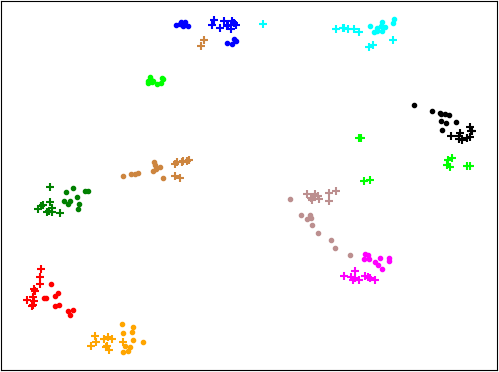
\includegraphics[width=\textwidth]{ChapterFour/tsne_triplet.png}
        \caption{CNN with triplet loss -- baseline 2}
        \label{fig:adv_signer_inv_tsne_b}
    \end{subfigure}
    %\hfill%
    \begin{subfigure}[t]{0.32\textwidth}
        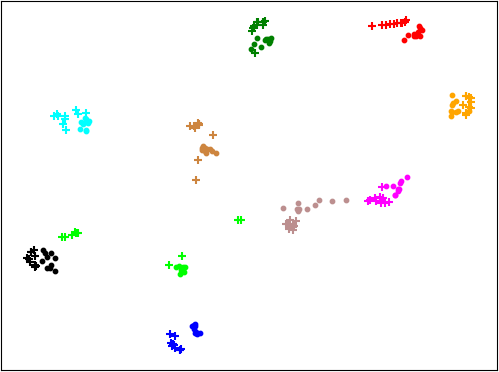
\includegraphics[width=\textwidth]{ChapterFour/tsne_proposed.png}
        \caption{Proposed model}
        \label{fig:adv_signer_inv_tsne_c}
    \end{subfigure}
    \caption{\centering Two-dimensional projection of the latent representation space using the t-distributed stochastic neighbor embedding (t-SNE). Markers $\bullet$ and $\textbf{+}$ represent 2 different test signers, while the different colors denote the 10 sign classes.}
    \label{fig:adv_signer_inv_tsne}
\end{figure}

%-------------------------------------------------------------------------
\subsection{Conclusion}
\label{sec:adv_signer_inv_conclusion}

This paper presents a novel adversarial training objective, based on representation learning and deep neural networks, specifically designed to tackle the signer-independent SLR problem. The underlying idea is to learn signer-invariant latent representations that preserve as much information as possible about the signs, while discarding the signer-specific traits that are irrelevant for sign recognition. For this purpose, we introduce  an adversarial training procedure for simultaneously training an \textit{encoder} and a \textit{sign-classifier} over the target sign variables, while preventing the latent representations of the \textit{encoder} to be predictive of the signer identities. To further discourage the underlying representations of retaining any signer-specific information, we propose an additional training objective that enforces the latent distributions of different signers to be as similar as possible.
Experimental results demonstrate the effectiveness of the proposed model in several SLR databases.

\section{Adversarial domain generalization for iris presentation attack detection}
\label{sec:adv_iris_attack}
In this section, we show how our adversarial domain generalization model for signer-invariant SLR (presented in \Secref{sec:adv_signer_inv}) can be adapted to a specific biometrics-related application.

\subsection{Introduction}
\label{sec:adv_iris_attack_intro}
Biometric recognition systems are considered reliable enough to be deployed in government and civilian applications. The shift from controlled samples acquisition to a more autonomous one increased the vulnerabilities of these systems. Unfortunately, presentation attack detection (PAD) measures had not grown robustly along with this quick evolution and several weak points can be exploited when performing unsupervised biometric identification as such in mobile biometrics, for example. Successful spoofing attempts have been made public in a matter of days, or even hours, after the release of high-tech devices equipped with biometric recognition. The iris recognition sensor of Samsung S8 was reportedly spoofed by German researchers by simply printing a photo of the authorised user and placing a contact lens in it (\citet{cccsamsung2017}). More recently, the quick hack of Samsung Galaxy S10 ultrasonic fingerprint sensor suggests no presentation attack detection measures of any kind. It is fair to conclude that industry does not share the same enthusiasm as academic community on anti-spoofing measures denoted by the good amount of research continuously produced (\citet{raghavendra2015VSIA,czajka2018irisPADreview,Galbally2019,scherhag2019}).

Fortunately, exceptions are starting to show in commercial products, like the recent case of the Apple iPhone `Face ID'' case~\footnote{www.biometricupdate.com/201812/android-devices-facial-recognition-fooled-by-3d-printed-head-but-not-face-id} or the FaceTec ZoOm® technology (\citet{facetec102019}). Undoubtedly this change is motivated and supported by initiatives that encourage the development and `open testing' of spoofing coutermeasures such as `The National Voluntary Laboratory Accreditation Program'' (NVLAP) from NIST \footnote{The NVLAP provides third-party accreditation to testing and calibration laboratories in response to legislative actions or requests from government agencies or private-sector organizations. NVLAP-accredited laboratories are assessed against the management and technical requirements from ISO/IEC 17025:2017.}

Nevertheless, research-wise there are still open problems to address. Here, we focus on the fact that most PAD techniques are based on falsely optimistic evaluation methodologies (\citet{sequeira2016realistic}): traditionally, the classification models are designed and then evaluated using datasets comprising \emph{bona fide} presentations and a specific species of presentation attack instruments (PAI). The case when a PAI in the test set is significantly different from the ones used for training is overlooked. What if such sample has a higher probability to circumvent the system than the ones drawn from the original training dataset? To solve this research question it is necessary to develop robust methods to cope with sophisticated and unseen attacks as our eventual intruders become more capable and successfully develop new spoofing techniques.

The aforementioned problem has in fact been addressed before regarding iris, fingerprint and face (often targeted under the open-set or anomaly detection contexts). However, it still remains a challenging topic. Despite the importance of iris as a biometric trait for recognition purposes, in our view, the study of iris PAD generalization problem to unseen PAI species (PAIS) has not been yet fully studied in literature.

The remainder of this section is organized as follows: i) we start by summarizing the related work on the topic (\Secref{sec:adv_iris_attack_rel_work}); ii) we formalize the problem and emphasize the necessary modifications that had to be done to the model presented in \Secref{sec:adv_signer_inv} to adapt it to this new application (\Secref{sec:adv_iris_attack_method}); iii) we present experimental results that confirm the effectiveness of the model (\Secref{sec:adv_iris_attack_experiments}); iv) we conclude this section with some final remarks (\Secref{sec:adv_iris_attack_conclusion}).

\subsection{Related work}
\label{sec:adv_iris_attack_rel_work}

Recent PAD methods in general, and iris-focused ones in particular, have demonstrated remarkable performances. However, a methodological limitation can be pointed as it is recurrently found that these results are obtained when training and test data comprise the same type of attacks, i.e.\ the same PAIS. This problem has been addressed and proved that the performance rates of these PAD methods typically decrease significantly when the PAIS is new to the system (\citet{marasco2011robustness,bowyer2014cosmetic,sequeira2016realistic}). This performance drop may be result of the large inter-`PAI-species' variability. A practical PAD system must operate in a `PAI-species'-independent scenario, which means that the type of PAIS of the test set must not be seen during the training routine of the models. This problem is one of the crucial problems for the development of real-world PAD systems and it has frequently been tackled in literature as an open-set or anomaly detection problem.

The pioneer work that raised the evaluation of PAD methods across different types and unseen PAIS appeared in the fingerprint domain with the work of \citet{marasco2011robustness}. \citet{rattani2015openset} and \citet{sequeira2015fingerprint}, despite using different approaches, both relied on the idea of enforcing the knowledge of the bona fide presentations over the attacks to better deal with unseen PAIS. \citet{bowyer2014cosmetic} studied the evaluation of a binary classification on contact lenses iris spoofing attacks. By using an unseen type on the test set the authors showed that using the same lens types in both the training and testing data can give a very misleading idea of the accuracy of the method.

A step forward was made by combining methodologies designed for print and contact lenses attack (\citet{sequeira2014ildmma}). Eventually, the construction of a new database comprising several types of iris PAIS (\citet{raghavendra2015VSIA}) allowed new evaluation scenarios. \citet{sequeira2016realistic} state that whenever a new PAIS is presented in the test step, the performance of the classifier drops significantly and that an improvement can be obtained when a one-class classifier is trained only with bona fide presentations.

One-class classification was also used for face by \citet{kittler2017faceanomaly}. With the rise of deep learning (DL) techniques, PAD methods have been proposed applying deep representations for iris, face and fingerprint (\citet{menotti2015deep,pinto2018counteracting}), following the same binary approach. Recent works investigate the robustness of DL fingerprint PAD methods to deal with unseen PAI species (\citet{tolosana2018towards}).

Until recently, most of the proposed approaches, either assume overly optimistic assumptions about the attacker  (binary classification approaches) or only use part of the data (and therefore, of the knowledge) available at training time to design the models (one-class approaches). Therefore, the goal of this work is to present an iris PAD method that uses the information of both bona fide and available attack presentations and is robust to unseen PAI species. This objective will be achieved by enforcing the learning of the task of distinguishing the bona fide from the attack presentations while at the same time ensuring the invariance between the different type of the PAI species.

\subsection{Methodology}
\label{sec:adv_iris_attack_method}
The approach adopted here coincides in most aspects with the one described in \Secref{sec:adv_signer_inv}, so we shall focus on describing the slight differences that exist. Now, the data consists of $\{\mX^{(\text{bf})}_i\}_{i=1}^{n_{\text{bf}}} \cup \{(\mX^{(\text{a})}_i,s_i)\}_{i=1}^{n_{\text{a}}}$, i.e.\ there is one set containing $n_{\text{bf}}$ bona fide examples and another one containing $n_{\text{a}}$ attack examples. Each attack example $\mX^{(\text{a})}_i$ is annotated with the corresponding PAI species label $s_i \in \{1,2,\dots,k\}$.

In this problem, we are solely interested in classifying samples as bona fide or attack, thus $h(\cdot;\vtheta_h)$ (formerly designated as sign-classifier) is now a binary classifier. More importantly, we want to obtain latent representations that are invariant to the PAI species, but the latent representations of bona fide examples should be easily separable from these. Thus, now, only the attack samples are fed through adversarial classifier $d(\cdot;\vtheta_d)$ (formerly designated as signer-classifier) and used for the adversarial training routine. For the same reason, the transfer loss $L_{\text{transfer}}$ approximating first-order statistics only applies to these samples too. \Figref{fig:adv_iris_model} presents the model architecture and hopefully makes the differences between this and our previous model even clearer.

\begin{figure*}[!hbt]
\centering
\tikzset{every picture/.style={line width=0.75pt}} %set default line width to 0.75pt

\scalebox{0.8}{

\tikzset{every picture/.style={line width=0.75pt}} %set default line width to 0.75pt

\begin{tikzpicture}[x=0.75pt,y=0.75pt,yscale=-1,xscale=1]
%uncomment if require: \path (0,637); %set diagram left start at 0, and has height of 637

%Shape: Rectangle [id:dp43448545781433445]
\draw  [draw opacity=0][fill={rgb, 255:red, 124; green, 163; blue, 233 }  ,fill opacity=0.27 ][dash pattern={on 4.5pt off 4.5pt}] (342,9) -- (521,9) -- (521,93.23) -- (342,93.23) -- cycle ;
%Shape: Rectangle [id:dp39844785350453726]
\draw   (373.93,38.03) -- (373.93,83.38) -- (359.01,83.38) -- (359.01,38.03) -- cycle ;
%Shape: Rectangle [id:dp5960148926786581]
\draw   (412.75,38.03) -- (412.75,83.38) -- (397.84,83.38) -- (397.84,38.03) -- cycle ;
%Shape: Rectangle [id:dp2968748699957451]
\draw   (451.86,45.72) -- (451.86,76.69) -- (436.94,76.69) -- (436.94,45.72) -- cycle ;
%Straight Lines [id:da38135442637321804]
\draw    (374.47,60.94) -- (396.84,60.84) ;
\draw [shift={(398.84,60.83)}, rotate = 539.75] [fill={rgb, 255:red, 0; green, 0; blue, 0 }  ][line width=0.75]  [draw opacity=0] (8.93,-4.29) -- (0,0) -- (8.93,4.29) -- cycle    ;

%Straight Lines [id:da5103446228646831]
\draw    (413.57,60.94) -- (435.94,60.84) ;
\draw [shift={(437.94,60.83)}, rotate = 539.75] [fill={rgb, 255:red, 0; green, 0; blue, 0 }  ][line width=0.75]  [draw opacity=0] (8.93,-4.29) -- (0,0) -- (8.93,4.29) -- cycle    ;

%Shape: Rectangle [id:dp21504155648063916]
\draw  [draw opacity=0][fill={rgb, 255:red, 255; green, 199; blue, 199 }  ,fill opacity=0.46 ][dash pattern={on 4.5pt off 4.5pt}] (342.06,123.9) -- (520.25,123.9) -- (520.25,208.13) -- (342.06,208.13) -- cycle ;
%Shape: Rectangle [id:dp5629086137047858]
\draw   (374.93,152.92) -- (374.93,198.28) -- (360.01,198.28) -- (360.01,152.92) -- cycle ;
%Shape: Rectangle [id:dp11383387176162141]
\draw   (414.75,152.92) -- (414.75,198.28) -- (399.84,198.28) -- (399.84,152.92) -- cycle ;
%Shape: Rectangle [id:dp8834314863600405]
\draw   (453.86,160.61) -- (453.86,191.59) -- (438.94,191.59) -- (438.94,160.61) -- cycle ;
%Straight Lines [id:da7960584409422926]
\draw    (375.47,175.84) -- (397.84,175.74) ;
\draw [shift={(399.84,175.73)}, rotate = 539.75] [fill={rgb, 255:red, 0; green, 0; blue, 0 }  ][line width=0.75]  [draw opacity=0] (8.93,-4.29) -- (0,0) -- (8.93,4.29) -- cycle    ;

%Straight Lines [id:da26603179330471005]
\draw    (414.57,175.84) -- (436.94,175.74) ;
\draw [shift={(438.94,175.73)}, rotate = 539.75] [fill={rgb, 255:red, 0; green, 0; blue, 0 }  ][line width=0.75]  [draw opacity=0] (8.93,-4.29) -- (0,0) -- (8.93,4.29) -- cycle    ;

%Straight Lines [id:da43094599217232044]
\draw [color={rgb, 255:red, 208; green, 2; blue, 27 }  ,draw opacity=1 ] [dash pattern={on 4.5pt off 4.5pt}]  (452.06,60.88) -- (552.61,60.84) ;
\draw [shift={(554.61,60.83)}, rotate = 539.98] [fill={rgb, 255:red, 208; green, 2; blue, 27 }  ,fill opacity=1 ][line width=0.75]  [draw opacity=0] (8.93,-4.29) -- (0,0) -- (8.93,4.29) -- cycle    ;

%Rounded Rect [id:dp20102262667247417]
\draw  [color={rgb, 255:red, 208; green, 2; blue, 27 }  ,draw opacity=1 ][dash pattern={on 4.5pt off 4.5pt}] (555.16,171.96) .. controls (555.16,170.16) and (556.62,168.71) .. (558.41,168.71) -- (621.75,168.71) .. controls (623.55,168.71) and (625,170.16) .. (625,171.96) -- (625,181.69) .. controls (625,183.48) and (623.55,184.94) .. (621.75,184.94) -- (558.41,184.94) .. controls (556.62,184.94) and (555.16,183.48) .. (555.16,181.69) -- cycle ;
%Straight Lines [id:da7107772326187543]
\draw [color={rgb, 255:red, 208; green, 2; blue, 27 }  ,draw opacity=1 ] [dash pattern={on 4.5pt off 4.5pt}]  (454.25,175.67) -- (552.78,176.37) ;
\draw [shift={(554.78,176.38)}, rotate = 180.41] [fill={rgb, 255:red, 208; green, 2; blue, 27 }  ,fill opacity=1 ][line width=0.75]  [draw opacity=0] (8.93,-4.29) -- (0,0) -- (8.93,4.29) -- cycle    ;

%Straight Lines [id:da7856916848123423]
\draw [color={rgb, 255:red, 208; green, 2; blue, 27 }  ,draw opacity=1 ] [dash pattern={on 4.5pt off 4.5pt}]  (147.5,197.88) -- (147.35,220.67) ;
\draw [shift={(147.33,222.67)}, rotate = 270.39] [fill={rgb, 255:red, 208; green, 2; blue, 27 }  ,fill opacity=1 ][line width=0.75]  [draw opacity=0] (8.93,-4.29) -- (0,0) -- (8.93,4.29) -- cycle    ;

%Straight Lines [id:da36002582240035363]
\draw [color={rgb, 255:red, 0; green, 0; blue, 0 }  ,draw opacity=1 ][line width=0.75]    (251.6,223.85) .. controls (253.27,225.52) and (253.27,227.18) .. (251.6,228.85) .. controls (249.93,230.52) and (249.93,232.18) .. (251.6,233.85) -- (251.6,236.85) -- (251.6,236.85)(248.6,223.85) .. controls (250.27,225.52) and (250.27,227.18) .. (248.6,228.85) .. controls (246.93,230.52) and (246.93,232.18) .. (248.6,233.85) -- (248.6,236.85) -- (248.6,236.85) ;


%Rounded Rect [id:dp28118263286951617]
\draw  [color={rgb, 255:red, 208; green, 2; blue, 27 }  ,draw opacity=1 ][dash pattern={on 4.5pt off 4.5pt}] (556.16,55.96) .. controls (556.16,54.16) and (557.62,52.71) .. (559.41,52.71) -- (622.75,52.71) .. controls (624.55,52.71) and (626,54.16) .. (626,55.96) -- (626,65.69) .. controls (626,67.48) and (624.55,68.94) .. (622.75,68.94) -- (559.41,68.94) .. controls (557.62,68.94) and (556.16,67.48) .. (556.16,65.69) -- cycle ;
%Straight Lines [id:da5356763271282314]
\draw [color={rgb, 255:red, 208; green, 2; blue, 27 }  ,draw opacity=1 ] [dash pattern={on 4.5pt off 4.5pt}]  (591.52,72.62) -- (591.71,101.6) ;

\draw [shift={(591.51,70.62)}, rotate = 89.63] [fill={rgb, 255:red, 208; green, 2; blue, 27 }  ,fill opacity=1 ][line width=0.75]  [draw opacity=0] (8.93,-4.29) -- (0,0) -- (8.93,4.29) -- cycle    ;
%Straight Lines [id:da9155638065763507]
\draw [color={rgb, 255:red, 208; green, 2; blue, 27 }  ,draw opacity=1 ] [dash pattern={on 4.5pt off 4.5pt}]  (590.12,188.42) -- (590.31,217.4) ;

\draw [shift={(590.11,186.42)}, rotate = 89.63] [fill={rgb, 255:red, 208; green, 2; blue, 27 }  ,fill opacity=1 ][line width=0.75]  [draw opacity=0] (8.93,-4.29) -- (0,0) -- (8.93,4.29) -- cycle    ;
%Straight Lines [id:da7191094178180941]
\draw [color={rgb, 255:red, 0; green, 0; blue, 0 }  ,draw opacity=1 ][line width=0.75]    (123.6,100.85) .. controls (125.27,102.52) and (125.27,104.18) .. (123.6,105.85) .. controls (121.93,107.52) and (121.93,109.18) .. (123.6,110.85) -- (123.6,113.85) -- (123.6,113.85)(120.6,100.85) .. controls (122.27,102.52) and (122.27,104.18) .. (120.6,105.85) .. controls (118.93,107.52) and (118.93,109.18) .. (120.6,110.85) -- (120.6,113.85) -- (120.6,113.85) ;


%Rounded Rect [id:dp5531536926433998]
\draw  [color={rgb, 255:red, 208; green, 2; blue, 27 }  ,draw opacity=1 ][dash pattern={on 4.5pt off 4.5pt}] (133.28,226.86) .. controls (133.28,224.77) and (134.98,223.07) .. (137.07,223.07) -- (235.08,223.07) .. controls (237.17,223.07) and (238.86,224.77) .. (238.86,226.86) -- (238.86,238.21) .. controls (238.86,240.31) and (237.17,242) .. (235.08,242) -- (137.07,242) .. controls (134.98,242) and (133.28,240.31) .. (133.28,238.21) -- cycle ;
%Straight Lines [id:da6744189660599909]
\draw [color={rgb, 255:red, 208; green, 2; blue, 27 }  ,draw opacity=1 ] [dash pattern={on 4.5pt off 4.5pt}]  (532.07,175.88) -- (532.47,268.68) -- (552.87,268.68) ;
\draw [shift={(554.87,268.68)}, rotate = 180] [fill={rgb, 255:red, 208; green, 2; blue, 27 }  ,fill opacity=1 ][line width=0.75]  [draw opacity=0] (8.93,-4.29) -- (0,0) -- (8.93,4.29) -- cycle    ;
\draw [shift={(532.07,175.88)}, rotate = 89.75] [color={rgb, 255:red, 208; green, 2; blue, 27 }  ,draw opacity=1 ][fill={rgb, 255:red, 208; green, 2; blue, 27 }  ,fill opacity=1 ][line width=0.75]      (0, 0) circle [x radius= 3.35, y radius= 3.35]   ;
%Rounded Rect [id:dp27586876312894315]
\draw  [color={rgb, 255:red, 208; green, 2; blue, 27 }  ,draw opacity=1 ][dash pattern={on 4.5pt off 4.5pt}] (554.76,264.36) .. controls (554.76,262.56) and (556.22,261.11) .. (558.01,261.11) -- (621.35,261.11) .. controls (623.15,261.11) and (624.6,262.56) .. (624.6,264.36) -- (624.6,274.09) .. controls (624.6,275.88) and (623.15,277.34) .. (621.35,277.34) -- (558.01,277.34) .. controls (556.22,277.34) and (554.76,275.88) .. (554.76,274.09) -- cycle ;
%Straight Lines [id:da05722319267703546]
\draw [color={rgb, 255:red, 208; green, 2; blue, 27 }  ,draw opacity=1 ] [dash pattern={on 4.5pt off 4.5pt}]  (590.37,280.67) -- (590.56,309.65) ;

\draw [shift={(590.36,278.67)}, rotate = 89.63] [fill={rgb, 255:red, 208; green, 2; blue, 27 }  ,fill opacity=1 ][line width=0.75]  [draw opacity=0] (8.93,-4.29) -- (0,0) -- (8.93,4.29) -- cycle    ;
%Shape: Rectangle [id:dp5258454923666749]
\draw   (683,267) -- (683,301) -- (671.91,301) -- (671.91,267) -- cycle ;
%Shape: Rectangle [id:dp18819058590818738]
\draw  [draw opacity=0][fill={rgb, 255:red, 226; green, 223; blue, 223 }  ,fill opacity=0.46 ][dash pattern={on 4.5pt off 4.5pt}] (110,9) -- (260.3,9) -- (260.3,93.23) -- (110,93.23) -- cycle ;
%Shape: Rectangle [id:dp12041639376004776]
\draw   (153.93,38.03) -- (153.93,83.38) -- (139.01,83.38) -- (139.01,38.03) -- cycle ;
%Shape: Rectangle [id:dp8185093400372612]
\draw   (192.75,38.03) -- (192.75,83.38) -- (177.84,83.38) -- (177.84,38.03) -- cycle ;
%Straight Lines [id:da46781806052292585]
\draw    (154.47,60.94) -- (176.84,60.84) ;
\draw [shift={(178.84,60.83)}, rotate = 539.75] [fill={rgb, 255:red, 0; green, 0; blue, 0 }  ][line width=0.75]  [draw opacity=0] (8.93,-4.29) -- (0,0) -- (8.93,4.29) -- cycle    ;

%Straight Lines [id:da8380691205174686]
\draw    (193.57,60.94) -- (215.94,60.84) ;
\draw [shift={(217.94,60.83)}, rotate = 539.75] [fill={rgb, 255:red, 0; green, 0; blue, 0 }  ][line width=0.75]  [draw opacity=0] (8.93,-4.29) -- (0,0) -- (8.93,4.29) -- cycle    ;

%Shape: Rectangle [id:dp7823549329526485]
\draw   (232.75,38.03) -- (232.75,83.38) -- (217.84,83.38) -- (217.84,38.03) -- cycle ;
%Straight Lines [id:da8112293131002832]
\draw    (232.57,60.94) -- (302,61) ;
\draw [shift={(302,61)}, rotate = 0.05] [color={rgb, 255:red, 0; green, 0; blue, 0 }  ][fill={rgb, 255:red, 0; green, 0; blue, 0 }  ][line width=0.75]      (0, 0) circle [x radius= 3.35, y radius= 3.35]   ;

%Straight Lines [id:da3383332186453154]
\draw    (74.69,60.46) -- (136.8,60.67) ;
\draw [shift={(138.8,60.68)}, rotate = 180.19] [fill={rgb, 255:red, 0; green, 0; blue, 0 }  ][line width=0.75]  [draw opacity=0] (8.93,-4.29) -- (0,0) -- (8.93,4.29) -- cycle    ;

%Shape: Rectangle [id:dp4074002721672936]
\draw  [draw opacity=0][fill={rgb, 255:red, 226; green, 223; blue, 223 }  ,fill opacity=0.46 ][dash pattern={on 4.5pt off 4.5pt}] (111,124) -- (261.3,124) -- (261.3,208.23) -- (111,208.23) -- cycle ;
%Shape: Rectangle [id:dp5490194067870466]
\draw   (154.93,153.03) -- (154.93,198.38) -- (140.01,198.38) -- (140.01,153.03) -- cycle ;
%Shape: Rectangle [id:dp5328143148819742]
\draw   (193.75,153.03) -- (193.75,198.38) -- (178.84,198.38) -- (178.84,153.03) -- cycle ;
%Straight Lines [id:da5553578784490631]
\draw    (155.47,175.94) -- (177.84,175.84) ;
\draw [shift={(179.84,175.83)}, rotate = 539.75] [fill={rgb, 255:red, 0; green, 0; blue, 0 }  ][line width=0.75]  [draw opacity=0] (8.93,-4.29) -- (0,0) -- (8.93,4.29) -- cycle    ;

%Straight Lines [id:da013990047318108267]
\draw    (194.57,175.94) -- (216.94,175.84) ;
\draw [shift={(218.94,175.83)}, rotate = 539.75] [fill={rgb, 255:red, 0; green, 0; blue, 0 }  ][line width=0.75]  [draw opacity=0] (8.93,-4.29) -- (0,0) -- (8.93,4.29) -- cycle    ;

%Shape: Rectangle [id:dp8533827475188887]
\draw   (233.75,153.03) -- (233.75,198.38) -- (218.84,198.38) -- (218.84,153.03) -- cycle ;
%Straight Lines [id:da9882205897592524]
\draw    (233.57,175.94) -- (358,175.67) ;
\draw [shift={(360,175.67)}, rotate = 539.87] [fill={rgb, 255:red, 0; green, 0; blue, 0 }  ][line width=0.75]  [draw opacity=0] (8.93,-4.29) -- (0,0) -- (8.93,4.29) -- cycle    ;

%Straight Lines [id:da787593595255915]
\draw    (75.69,175.46) -- (137.8,175.67) ;
\draw [shift={(139.8,175.68)}, rotate = 180.19] [fill={rgb, 255:red, 0; green, 0; blue, 0 }  ][line width=0.75]  [draw opacity=0] (8.93,-4.29) -- (0,0) -- (8.93,4.29) -- cycle    ;

%Shape: Rectangle [id:dp9669269547137105]
\draw  [draw opacity=0][fill={rgb, 255:red, 226; green, 223; blue, 223 }  ,fill opacity=0.46 ][dash pattern={on 4.5pt off 4.5pt}] (110,256) -- (260.3,256) -- (260.3,340.23) -- (110,340.23) -- cycle ;
%Shape: Rectangle [id:dp042461560729392334]
\draw   (153.93,267.03) -- (153.93,312.38) -- (139.01,312.38) -- (139.01,267.03) -- cycle ;
%Shape: Rectangle [id:dp05976855107797907]
\draw   (192.75,267.03) -- (192.75,312.38) -- (177.84,312.38) -- (177.84,267.03) -- cycle ;
%Straight Lines [id:da15536321808735676]
\draw    (154.47,289.94) -- (176.84,289.84) ;
\draw [shift={(178.84,289.83)}, rotate = 539.75] [fill={rgb, 255:red, 0; green, 0; blue, 0 }  ][line width=0.75]  [draw opacity=0] (8.93,-4.29) -- (0,0) -- (8.93,4.29) -- cycle    ;

%Straight Lines [id:da390775000910931]
\draw    (193.57,289.94) -- (215.94,289.84) ;
\draw [shift={(217.94,289.83)}, rotate = 539.75] [fill={rgb, 255:red, 0; green, 0; blue, 0 }  ][line width=0.75]  [draw opacity=0] (8.93,-4.29) -- (0,0) -- (8.93,4.29) -- cycle    ;

%Shape: Rectangle [id:dp6405433268349929]
\draw   (232.75,267.03) -- (232.75,312.38) -- (217.84,312.38) -- (217.84,267.03) -- cycle ;
%Straight Lines [id:da12900931641427915]
\draw    (74.69,289.46) -- (136.8,289.67) ;
\draw [shift={(138.8,289.68)}, rotate = 180.19] [fill={rgb, 255:red, 0; green, 0; blue, 0 }  ][line width=0.75]  [draw opacity=0] (8.93,-4.29) -- (0,0) -- (8.93,4.29) -- cycle    ;

%Straight Lines [id:da6895522275561663]
\draw [color={rgb, 255:red, 208; green, 2; blue, 27 }  ,draw opacity=1 ] [dash pattern={on 4.5pt off 4.5pt}]  (186.17,198.54) -- (186.01,221.33) ;
\draw [shift={(186,223.33)}, rotate = 270.39] [fill={rgb, 255:red, 208; green, 2; blue, 27 }  ,fill opacity=1 ][line width=0.75]  [draw opacity=0] (8.93,-4.29) -- (0,0) -- (8.93,4.29) -- cycle    ;

%Straight Lines [id:da7826731128924016]
\draw [color={rgb, 255:red, 208; green, 2; blue, 27 }  ,draw opacity=1 ] [dash pattern={on 4.5pt off 4.5pt}]  (226.17,197.88) -- (226.01,220.67) ;
\draw [shift={(226,222.67)}, rotate = 270.39] [fill={rgb, 255:red, 208; green, 2; blue, 27 }  ,fill opacity=1 ][line width=0.75]  [draw opacity=0] (8.93,-4.29) -- (0,0) -- (8.93,4.29) -- cycle    ;

%Straight Lines [id:da04218018142765656]
\draw [color={rgb, 255:red, 208; green, 2; blue, 27 }  ,draw opacity=1 ] [dash pattern={on 4.5pt off 4.5pt}]  (147.49,243.87) -- (147.33,266.67) ;

\draw [shift={(147.5,241.88)}, rotate = 90.39] [fill={rgb, 255:red, 208; green, 2; blue, 27 }  ,fill opacity=1 ][line width=0.75]  [draw opacity=0] (8.93,-4.29) -- (0,0) -- (8.93,4.29) -- cycle    ;
%Straight Lines [id:da31456133747342974]
\draw [color={rgb, 255:red, 208; green, 2; blue, 27 }  ,draw opacity=1 ] [dash pattern={on 4.5pt off 4.5pt}]  (185.49,243.87) -- (185.33,266.67) ;

\draw [shift={(185.5,241.88)}, rotate = 90.39] [fill={rgb, 255:red, 208; green, 2; blue, 27 }  ,fill opacity=1 ][line width=0.75]  [draw opacity=0] (8.93,-4.29) -- (0,0) -- (8.93,4.29) -- cycle    ;
%Straight Lines [id:da5649357265644332]
\draw [color={rgb, 255:red, 208; green, 2; blue, 27 }  ,draw opacity=1 ] [dash pattern={on 4.5pt off 4.5pt}]  (226.49,243.87) -- (226.33,266.67) ;

\draw [shift={(226.5,241.88)}, rotate = 90.39] [fill={rgb, 255:red, 208; green, 2; blue, 27 }  ,fill opacity=1 ][line width=0.75]  [draw opacity=0] (8.93,-4.29) -- (0,0) -- (8.93,4.29) -- cycle    ;
%Straight Lines [id:da21749981772402482]
\draw    (302,176) -- (302,66.83) ;
\draw [shift={(302,64.83)}, rotate = 450] [fill={rgb, 255:red, 0; green, 0; blue, 0 }  ][line width=0.75]  [draw opacity=0] (8.93,-4.29) -- (0,0) -- (8.93,4.29) -- cycle    ;

%Straight Lines [id:da8956250937163148]
\draw [color={rgb, 255:red, 0; green, 0; blue, 0 }  ,draw opacity=1 ][line width=0.75]    (123.6,224.85) .. controls (125.27,226.52) and (125.27,228.18) .. (123.6,229.85) .. controls (121.93,231.52) and (121.93,233.18) .. (123.6,234.85) -- (123.6,237.85) -- (123.6,237.85)(120.6,224.85) .. controls (122.27,226.52) and (122.27,228.18) .. (120.6,229.85) .. controls (118.93,231.52) and (118.93,233.18) .. (120.6,234.85) -- (120.6,237.85) -- (120.6,237.85) ;


%Straight Lines [id:da9131455128555723]
\draw [color={rgb, 255:red, 0; green, 0; blue, 0 }  ,draw opacity=1 ][line width=0.75]    (251.6,100.85) .. controls (253.27,102.52) and (253.27,104.18) .. (251.6,105.85) .. controls (249.93,107.52) and (249.93,109.18) .. (251.6,110.85) -- (251.6,113.85) -- (251.6,113.85)(248.6,100.85) .. controls (250.27,102.52) and (250.27,104.18) .. (248.6,105.85) .. controls (246.93,107.52) and (246.93,109.18) .. (248.6,110.85) -- (248.6,113.85) -- (248.6,113.85) ;


%Straight Lines [id:da34712918534938386]
\draw [color={rgb, 255:red, 0; green, 0; blue, 0 }  ,draw opacity=1 ][line width=0.75]    (679.6,310.85) .. controls (681.27,312.52) and (681.27,314.18) .. (679.6,315.85) .. controls (677.93,317.52) and (677.93,319.18) .. (679.6,320.85) -- (679.6,323.85) -- (679.6,323.85)(676.6,310.85) .. controls (678.27,312.52) and (678.27,314.18) .. (676.6,315.85) .. controls (674.93,317.52) and (674.93,319.18) .. (676.6,320.85) -- (676.6,323.85) -- (676.6,323.85) ;


%Straight Lines [id:da3483077683758504]
\draw    (302,61) -- (358,61) ;
\draw [shift={(360,61)}, rotate = 180] [fill={rgb, 255:red, 0; green, 0; blue, 0 }  ][line width=0.75]  [draw opacity=0] (8.93,-4.29) -- (0,0) -- (8.93,4.29) -- cycle    ;


% Text Node
\draw (58.68,60.11) node   {$\boldsymbol{X}^{(\text{bf})}_{i}$};
% Text Node
\draw (61.35,230.89) node  [align=left] {\textbf{{\large .}}\\\textbf{{\large .}}\\\textbf{{\large .}}};
% Text Node
\draw (448.89,20.95) node   {$h(\boldsymbol{z}\mathrm{;}\boldsymbol{\theta} _{h})$};
% Text Node
\draw (456.63,134.64) node   {$d(\boldsymbol{z}\mathrm{;}\boldsymbol{\theta} _{d})$};
% Text Node
\draw (589.25,177.03) node   {${\textstyle \mathcal{\textcolor[rgb]{0.82,0.01,0.11}{L}}\textcolor[rgb]{0.82,0.01,0.11}{_{\mathrm{species}}}}$};
% Text Node
\draw (495.39,48.2) node   {$p( \ry \mid \boldsymbol{z}_{i} ;\boldsymbol{\theta} _{h})$};
% Text Node
\draw (249.56,53.01) node   {$\boldsymbol{z}_{i}$};
% Text Node
\draw (183.66,231.92) node   {${\textstyle \mathcal{\textcolor[rgb]{0.82,0.01,0.11}{L}}\textcolor[rgb]{0.82,0.01,0.11}{_{\mathrm{transfer}}}}$};
% Text Node
\draw (590.25,61.03) node   {${\textstyle \mathcal{\textcolor[rgb]{0.82,0.01,0.11}{L}}\textcolor[rgb]{0.82,0.01,0.11}{_{\mathrm{task}}}}$};
% Text Node
\draw (593,110.17) node   {$y_{i}$};
% Text Node
\draw (591.6,225.97) node   {$s_{j}$};
% Text Node
\draw (588.85,268.43) node   {${\textstyle \mathcal{\textcolor[rgb]{0.82,0.01,0.11}{L}}\textcolor[rgb]{0.82,0.01,0.11}{_{\mathrm{adv}}}}$};
% Text Node
\draw (591.85,318.22) node   {$\mathcal{U}(\mathrm{s})$};
% Text Node
\draw (738,283.5) node  [align=left] {{\scriptsize Fully-connected layer}};
% Text Node
\draw (52.96,329) node [scale=0.7]  {$\mathnormal{s_{k} \neq s_{j}}$};
% Text Node
\draw (495.89,163.7) node   {$p( \rs \mid \boldsymbol{z}_{j} ;\boldsymbol{\theta} _{d})$};
% Text Node
\draw (232.7,17.44) node   {$g(\boldsymbol{X}\mathrm{;}\boldsymbol{\theta} _{g})$};
% Text Node
\draw (59.68,175.11) node   {$\boldsymbol{X}^{(\text{a})}_{j}$};
% Text Node
\draw (250.56,168.01) node   {$\boldsymbol{z}_{j}$};
% Text Node
\draw (233.7,132.44) node   {$g(\boldsymbol{X}\mathrm{;}\boldsymbol{\theta} _{g})$};
% Text Node
\draw (58.68,289.11) node   {$\boldsymbol{X}^{(\text{a})}_{k}$};
% Text Node
\draw (234.7,329.44) node   {$g(\boldsymbol{X}\mathrm{;}\boldsymbol{\theta} _{g})$};
% Text Node
\draw (725,316.5) node  [align=left] {{\scriptsize Shared weights}};
\end{tikzpicture}
}
\caption{Block diagram of the proposed species-invariant neural network.}
\label{fig:adv_iris_model}
\end{figure*}


\subsection{Experiments}
\label{sec:adv_iris_attack_experiments}
We use the Visible Spectrum Iris Artefact (VSIA) Database (\citet{raghavendra2015VSIA}) in our experiments. This dataset comprises five different presentations combining print and electronic screen attacks: i) Print Attack (PA); ii) iPad Electronic Screen Attack (ESA); iii) Samsung Galaxy Tab ESA; (iv) combined PA \& ESA using iPad; and v) combined PA \& ESA using Samsung Pad. The methods are evaluated by leaving out one PAI species for testing. The training set is therefore divided in one specie for validation and the remaining used for training. Also the same set of samples are used for testing across the different experiments to allow precise comparison of the results. Following \citet{sequeira2016realistic}, weighted local binary pattern features (wLBP, \citet{zhang2010contact}) were extracted in a preprocessing step and fed as input to the network, which in this case consists of an MLP.

Our model was compared to a baseline consisting of the same classifier without the PAI species classifier and adversarial training and to an SVM operating on top of the same wLBP features (\citet{sequeira2016realistic}). Results are in \Tableref{tab:pad_accuracy}. Comparing the accuracy for each attack, it can be observed that uniquely replacing the SVM with an MLP does not result in an improvement. This can be explained by the fact that the dataset has a very limited size and therefore the MLP method tends to overfit due to the lack of training samples. It was not for no reason that SVMs ruled for a long time in the pattern recognition domain. However, the proposed adversarial approach outperformed the SVM for most attacks and on average as well.

For further results and details about the experiments, please see \citet{AdvInvAttack}.

\begin{table}[t]
    \centering
    \begin{small}
        \begin{tabular}{c|c c c c c:c}
            & Attack i)
            & Attack ii)
            & Attack iii)
            & Attack iv)
            & Attack v)
            & Avg. \\ \hline

            wLBP+SVM~\cite{sequeira2016realistic}
            &78.85     &90.39     &\bf 98.08 &\bf 95.68 & 97.12     & 92.02 \\
            Baseline wLBP+MLP
            &78.00     &\bf 93.00  &94.50    &90.00   &95.50     &90.20 \\
            Proposed wLBP+$\text{MLP}_\text{adv}$
            &\bf82.00  &\bf 93.00  &98.00   &94.50   &\bf 97.50  &\bf 93.00
        \end{tabular}
    \end{small}
    \caption{Presentation attack detection accuracy (\%) in the VSIA dataset.}
    \label{tab:pad_accuracy}
\end{table}

\subsection{Conclusion}
\label{sec:adv_iris_attack_conclusion}
This work proposed a method to improve the robustness and generalization capacity of an iris PAD method to new attacks. The goal of the proposed model is to learn latent representations invariant to the PAI species that preserve relevant information about the PAD properties while discarding the `PAI-species'-specific aspects that may hamper the PAD classification task. The proposed regularization strategies made the PAD method `PAI-species'-independent and robust to new test PAIS.
The experiments were based in comparing a baseline MLP and an MLP trained with adversarial strategies using as input highly discriminative features (wLBP) extracted from the images. When comparing the baseline MLP to an SVM classifier the results are quite similar or even worse. This can be explained simply by the fact that the dataset has a very limited size and the MLP method will overfit.
However, applying the adversarial regularization strategy significantly improved the PAD robustness of the method. The obtained results clearly suggest that the application of deep learning techniques with additional strategies will provide breakthroughs in this challenge.

\section{DeSIRe: Deep Signer-Invariant Representations for Sign Language Recognition}
\label{sec:desire}

\subsection{Introduction}
In \Secref{sec:adv_signer_inv}, we introduced a method for domain generalization which uses adversarial neural networks to align the marginal distributions of multiple source domains. The method showed promising results for both visual (\Secref{sec:adv_signer_inv}) and non-visual data (\Secref{sec:adv_iris_attack}). Here, we again focus our attention on vision problems and, specifically, on solving the problem of signer-independent SLR.

To specifically tackle the signer-independent SLR problem, we now present DeSIRe, a novel deep neural network that aims to learn \textbf{De}ep \textbf{S}igner-\textbf{I}nvariant \textbf{Re}presentations. The underlying idea is to explicitly enforce the model to automatically learn highly discriminative signer-invariant feature representations from the data by aligning and regularizing conditional distributions in a latent space. To accomplish this goal, the DeSIRe model consists of two main modules or components, namely a conditional variational autoencoder (CVAE) and a classifier. Specifically, the main task of the CVAE is to explicitly impose signer independence on the learned latent representations. This is achieved by encouraging the CVAE to learn latent representations whose conditional posterior distribution, given the image and its sign label, is independent of the signer identity. Accordingly, the learned latent representations will preserve as much information as possible about the class (sign), and discard the irrelevant parts that are signer-specific. In addition, the CVAE acts as a teacher model for the classifier since the distribution over latent representations is used to regularize the hidden representations of the classifier. These hidden representations are then fed into a multilayer perceptron (MLP) for sign recognition. The result is a signer-independent model robust to new test signers.

The remainder of this section is organized as follows: The proposed signer-independent deep neural network along with the proposed loss function and regularization schemes are fully described in Section \ref{sec:proposed_method}. Section \ref{sec:experiments} reports the experimental evaluation of the proposed methodology, in which a comparison with state-of-the-art and baseline methods is performed. Finally, conclusions and some topics for future work are presented in Section \ref{sec:conclusion}.

\subsection{The DeSIRe model}

The high-level block diagram of the proposed DeSIRe model is depicted in Figure \ref{fig:model_archi}. As it is possible to observe, it is composed by a CVAE and a classifier. In our model, the underlying idea of the CVAE is to learn an invertible mapping to a space where the signer-specific information is disentangled from the discriminative properties of the sign class. The CVAE can be thought as a teacher model for the classifier, as the distribution over latent representations $\rvz$ is used to regularize the hidden representations $\tilde{\vz}$ of the classifier. These hidden representations $\tilde{\vz}$ are then fed into a multilayer perceptron (MLP) for a robust signer-independent SLR.

Specifically, the CVAE consists of an encoder and a decoder network, parameterized by $\vtheta_e$ and $\vtheta_d$, respectively. The purpose of the encoder network is to learn a distribution $q(\rvz \mid \rmX, \ry, \rs; \vtheta_e)$ which approximates the true posterior distribution of the latent code $\rvz$ given the image $\rmX$, the class label $\ry$ and the signer identity $\rs$. By conditioning the posterior distribution on $\rs$ and $\ry$, we are empowering the encoder by learning a domain and class-dependent transformation. Here, the key idea is to learn latent codes whose conditional posterior distribution is independent of the signer identity, that is $q(\rvz \mid \rmX, \ry, \rs; \vtheta_e) \equiv q(\rvz \mid \rmX, \ry; \vtheta_e)$. Equivalently, latent codes are conditionally independent of the signer identity given the image and its class if and only if:
\begin{equation}
    \label{eq:independence}
    q(\rvz \mid \rmX, \ry, \rs=s; \vtheta_e) \equiv q(\rvz \mid \rmX, \ry, \rs=s'; \vtheta_e),
\end{equation}
for any two distinct signers $s$ and $s'$. In order to promote this signer-independence property, the loss function includes a term that penalizes deviations from this equality. However, if no additional care is taken, this condition would compete with the reconstruction objective since reconstructing an image implies preserving as much information about the image as possible, including signer-specific information. Therefore, the signer identity is sampled uniformly at random and fed as an additional input to the decoder network. By this mean, the decoder shall provide a disentangled representation of the signer identity which, combined with the signer-invariant latent code $\vz$, will be used to reconstruct the original sample.

Intuitively, as the latent vector $\vz$ is sampled from $q(\rvz \mid \rmX, \ry, \rs; \vtheta_e)$, the latent representations $\vz$ will preserve as much information as possible about the class (sign), and discard the irrelevant parts that are characteristic of each signer. The loss function is defined in such a manner that it encourages similarity between the latent codes $\vz$ and the hidden representations $\tilde{\vz}$ of the classifier module. The classifier is then trained on these signer-invariant representations for a robust signer-independent SLR. Formally, $h(\cdot; \vtheta_h): \gZ \mapsto \gY$ represents our task-specific function, parameterized by $\vtheta_h$, that maps from the hidden representation to the predicted sign class $\hat{y}$, and $g(\cdot; \vtheta_g): \gX \mapsto \gZ$ denotes an encoding function, parameterized by $\vtheta_g$, that maps the input images to the corresponding hidden representations.

\subsubsection{Loss function}
\label{sec:desire_loss}
Training the proposed DeSIRe model is achieved by minimizing the following loss function with respect to parameters $\Theta=\{\vtheta_{e},\vtheta_{d},\vtheta_{g},\vtheta_{h}\}$:
\begin{equation}
    L(\Theta) \triangleq L_{\text{CVAE}}(\vtheta_{d},\vtheta_{e}) + \lambda_{1} L_{\text{emb}}(\vtheta_{e},\vtheta_{f}) + \lambda_{2} L_{\text{class}}(\vtheta_{f},\vtheta_{g}),
\end{equation}
where $\lambda_{1},\lambda_{2}\geq 0$ are the weights that control the interaction between the loss terms.

The ultimate goal of the CVAE loss, $L_{\text{CVAE}}$, is to explicitly impose signer independence by learning latent representations which are conditionally independent from the signer identity. In this regard, $L_{\text{CVAE}}$ is defined by:
\begin{equation}
    L_{\text{CVAE}}(\vtheta_{d},\vtheta_{e}) \triangleq L_{\text{rec}}(\vtheta_{d}) + \alpha_{1} L_{\text{prior}}(\vtheta_{e}) + \alpha_{2} L_{\text{signer\_inv}}(\vtheta_{e}),
\end{equation}
where $\alpha_{1},\alpha_{2}\geq 0$ are hyperparameters that control the relative importance of each loss term. The first two terms, $L_{\text{rec}}$ and $L_{\text{prior}}$, correspond to the loss function of a standard CVAE, containing some special modifications for promoting signer-independence in the latent space. The reconstruction loss $L_{\text{rec}}$ encourages the decoder to learn how to reconstruct the input data $\rmX$. For the decoder, we assume that the conditional likelihood of the data $\rmX$ given the latent code $\rvz$ and the signer identity $\rs$ follows a Gaussian distribution. Accordingly, as explained in \Secref{sec:background_cvae}, the reconstruction loss corresponds to the mean-squared error between a training image and a generated image. Here, however, instead of working with pairs of ground-truth images together with their respective reconstructions, we make a slight modification that further promotes signer-invariant encodings. Let $\mX^{(r)}_{y,s}$ denote the $r$-th image of signer $s$ and sign class $y$. Specifically, we compute the mean-squared error between the $j$-th $d$-dimensional training image $\mX^{(r_{j})}_{y_{j},s_{j}}$ and the generated $d$-dimensional image $\vmu_d(\vz_{i},s_{j}; \theta_{d})$ which is produced by the decoder when fed with the encoding $\vz_{i}$ of the $i$-th training image $\mX^{(r_{i})}_{y_{i},s_{i}}$ and with the signer identity $s_j$ of the $j$-th training image:
\begin{equation}
    \label{eq:loss_rec}
    L_{\text{rec}}(\vtheta_{d}) \triangleq \frac{1}{n d} \sum_{i=1}^{n}||\mX^{(r_{j})}_{y_{j},s_{j}}-\vmu_d(\vz_{i},s_{j}; \theta_{d})||^2_2,
\end{equation}
where $y_{j}=y_{i}$, $\vz_{i}$ is sampled from $q(\rvz_{i} \mid \mX^{(r_{i})}_{y_{i},s_{i}}, y_{i}, s_{i}; \theta_e)$ using the reparameterization trick \plaineqref{eq:reparam_trick}, $s_{j}$ is sampled from a distribution $w(\rs \mid s_{i})$, defined below, and $r_{j}$ is sampled uniformly from the set of available repetitions:
\begin{equation}
    w(\rs \mid s_{i}) \triangleq
    \begin{cases}
        1-\rho, \quad \rs=s_{i}, \\
        \frac{\rho}{k-1}, \quad \rs \in \{1,2,\dots,k\} \setminus \lbrace s_{i} \rbrace.
    \end{cases}
\end{equation}
Here, as before, $\{1,2,\dots,k\}$ is the set of signer identities in the training data and $\rho \in [0, 1]$ is a hyperparameter. By sampling the identity $s_{j}$ of the ground-truth image from $w(\rs \mid s_{i})$, decoder will be trained to reconstruct an image of a different subject (but same sign class) than the one that was used to produce the encoding. This will happen in a proportion $\rho$ of the cases. This procedure further discourages the latent codes to preserve signer-specific information and therefore aims to reduce inter-signer variability. On the other hand, by sampling the sign repetition $r_{j}$, the decoder will also be trained to reconstruct a distinct image of the same person and sign class as the image that produced the encoding. Here, the purpose is to gain robustness to intra-signer variability. Although less problematic than the former, this type of variability is also relevant since the same signer does not always repeat the same sign in exactly the same way. Moreover, different image acquisition conditions (e.g.\ background, illumination, distance to the camera, etc.) from one repetition to another also result in intra-signer variability.

The $L_{\text{prior}}$ term corresponds to the KL divergence between the posterior and the prior as commonly used in a standard CVAE:
\begin{align}
    \label{eq:loss_prior}
    L_{\text{prior}}(\vtheta_{e}) &\triangleq \frac{1}{nl} \sum_{i=1}^n \KL(q(\rvz_{i} \mid \mX^{(r_{i})}_{y_{i},s_{i}}, y_{i}, s_{i}; \vtheta_e) || \gN(\rvz_{i}; 0, \mI)) \nonumber\\
    &= \frac{1}{2nl} \sum_{i=1}^n \sum_{j=1}^l \left(\mu_{e,i,j}^2 + \sigma_{e,i,j}^2 -1 - \log \sigma_{e,i,j}^2\right),
\end{align}
where $l$ is the dimension of the latent space and $\mu_{e,i,j}$ and $\sigma_{e,i,j}$ denote the $j$-th elements of the vectors $\vmu_{e}(\mX_i, y_i, s_i; \vtheta_e)$ and $\vsigma_{e}(\mX_i, y_i, s_i; \vtheta_e)$, respectively.

An explicit constraint for signer-independence is also introduced in the CVAE loss function. $L_{\text{signer\_inv}}$ encourages the conditional posterior distribution of latent codes $\rvz$, given the image $\rmX$ and its class $\ry$, to be independent of the signer identity $\rs$. This loss is defined as the KL divergence between conditional posterior distributions of $\rvz$, conditioned on the same class but also on different signer identities:
\begin{align}
    \label{eq:loss_signer_inv}
    \mathcal{L}_{\text{signer\_inv}}(\vtheta_{e}) &\triangleq \frac{1}{nl} \sum_{i=1}^{n}\KL\left(q(\rvz_{i} \mid \mX^{(r_{i})}_{y_{i},s_{i}}, y_{i}, s_{i}; \vtheta_e) \big| \big| q(\rvz_{k} \mid \mX^{(r_{k})}_{y_{k},s_{k}}, y_{k}, s_{k}; \vtheta_e)\right) \nonumber\\
    &=\frac{1}{2nl}~\sum_{i=1}^{n}\sum_{j=1}^{l} \Biggl(\frac{(\mu_{e,i,j} - \mu_{e,k,j})^2}{\sigma_{e,k,j}^2} + \frac{\sigma_{e,i,j}^2}{\sigma_{e,k,j}^2} -1 + \log \sigma_{e,k,j}^2 - \log \sigma_{e,i,j}^2 \Biggr),
\end{align}
where $y_{k}=y_{i}$ and $s_k$ is sampled uniformly from $\{1,2,\dots,k\} \setminus \lbrace s_i \rbrace$. The second equality follows from the fact that both distributions are Gaussian and so their KL divergence may be computed analytically, as in \eqref{eq:loss_prior}.

The signer-invariant latent representations $\rvz$ learned by the CVAE are then used to regularize the hidden representations $\vh$ of the classifier. Such regularization is promoted by the $L_{\text{emb}}$ loss term, which encourages the latent representations of the CVAE and the classifier to be as similar as possible. Following this idea, the embedding loss $L_{\text{emb}}$ is defined to minimize the expected mean-squared error between $\rvz$ and $\vh$, that is:
\begin{equation}
    \label{eq:emb_loss}
    L_{\text{emb}}(\vtheta_e, \vtheta_g) \triangleq \frac{1}{nl} \sum_{i=1}^{n} \E_{\rvz_{i} \sim q(\rvz \mid \mX^{(r_{i})}_{y_{i},s_{i}}, y_{i}, s_{i}; \vtheta_e)}||\rvz_i-\tilde{\vz}_i||^2.
\end{equation}
In practice, we replace \eqref{eq:emb_loss} by its Monte Carlo approximation with one sample, which yields:
\begin{equation}
    L_{\text{emb}}(\vtheta_e, \vtheta_g) \approx \frac{1}{nl} \sum_{i=1}^{n}||\vz_i-\tilde{\vz}_i||^2,
\end{equation}
where $\vz_i$ is sampled from $q(\rvz_{i} \mid \mX^{(r_{i})}_{y_{i},s_{i}}, y_{i}, s_{i}; \vtheta_e)$, again using the reparameterization trick \plaineqref{eq:reparam_trick}. This approximation has an extra regularizing effect on the classifier network, by introducing some stochastic noise in its training routine.

Finally, the classification loss, $L_{\text{class}}$, trains the model to predict the output sign labels and corresponds to the categorical cross-entropy, defined by:
\begin{equation}
    \label{eq:desire_loss_class}
    L_{\text{class}}(\vtheta_{g},\vtheta_{h}) \triangleq -\frac{1}{n} \sum_{i=1}^{n}\log p(y_{i} \mid \mX^{(r_{i})}_{y_{i}, s_{i}};\vtheta_{g},\vtheta_{h}),
\end{equation}
where $p(y \mid \mX; \vtheta_{g},\vtheta_{h})$ is the predicted probability that a given image $\mX$ belongs to its ground-truth class $y$, according to the current classifier parameters $\vtheta_{g}$ and $\vtheta_{h}$.

A full schematic of the DeSIRe model including all loss terms is presented in Appendix~\ref{sec:desire_arch}. A few training heuristics which were employed to improve the training of the model are described in Appendix~\ref{sec:desire_training_strat}.

\subsubsection{Inference}
\label{sec:desire_inference}
During the training stage, the CVAE module plays the role of a teacher model for the classifier. Accordingly, the CVAE can be discarded at inference time. Therefore, inference in DeSIRe simply consists of a forward pass through the classifier network, such that $\hat{y} \triangleq \argmax h(\tilde{\vz}; \vtheta_h)$ and $\tilde{\vz} = g(\mX; \vtheta_g)$.

\subsection{Experiments}
\label{sec:desire_experiments}

For reproducibility purposes, For reproducibility purposes, the source code as well as the weights of the trained models are publicly available online\footnote{https://github.com/pmmf/DeSIRe}. Further details about the training of the model and

\subsubsection{Datasets}
We use the same datasets and follow the same experimental protocol as in our previous model, described in \Secref{sec:adv_signer_inv_experiments}. Additionally, we also evaluate our model in a subset of the CorSiL database.

CorSiL is a dataset for Portuguese sign language and expressiveness recognition. Its SLR subset comprises 182 isolated signs and 40 continuous sequences, which we have further refined by selecting 31 isolated signs from 11 distinct signers, with each sign being repeated 3 times for each signer. All signs
were performed in a free and natural signing environment. This variability, together with the large number of sign classes, makes this dataset a
challenging one. A few samples are shown in \Figref{fig:corsil}. We use six signers for training, one signer for validation and the remaining four signers are used for testing.

\begin{figure}[t]
    \centering
    \begin{minipage}[t]{0.3\columnwidth}
        \begin{tikzpicture}[spy using outlines={circle,red,magnification=4,size=1.4cm, connect spies}]
            \node {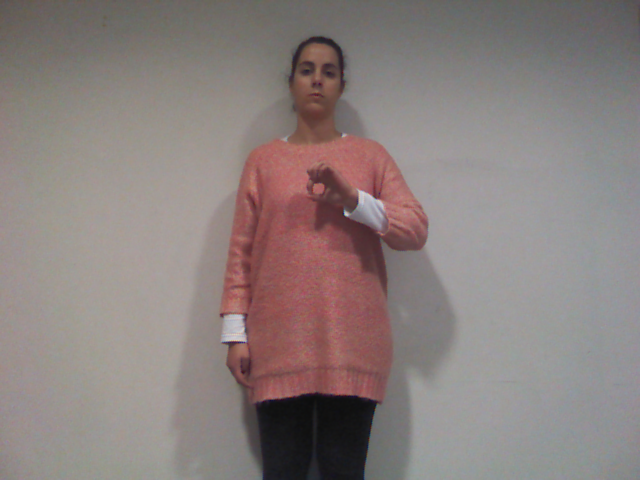
\includegraphics[interpolate=true, height=0.50\columnwidth]{ChapterFour/1_psl.png}};
            \spy on (0.05,0.23) in node [left] at (1.6,0.9);
        \end{tikzpicture}
    \end{minipage}
    \hspace{0.00mm}
    \begin{minipage}[t]{0.3\columnwidth}
        \begin{tikzpicture}[spy using outlines={circle,red,magnification=4,size=1.4cm, connect spies}]
            \node {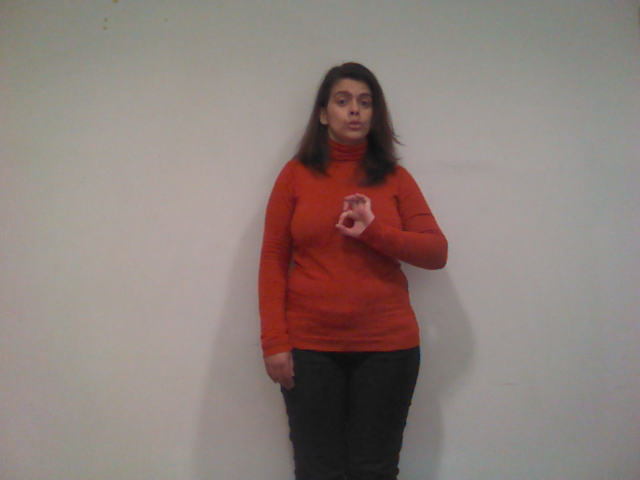
\includegraphics[interpolate=true, height=0.50\columnwidth]{ChapterFour/2_psl.png}};
            \spy on (0.16,0.07) in node [left] at (1.6,0.9);
        \end{tikzpicture}
    \end{minipage}
    \hspace{0.00mm}
    \begin{minipage}[t]{0.3\columnwidth}
        \begin{tikzpicture}[spy using outlines={circle,red,magnification=4,size=1.4cm, connect spies}]
            \node {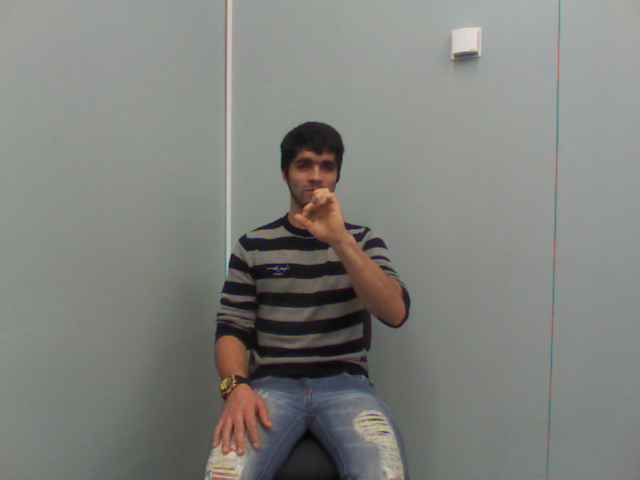
\includegraphics[interpolate=true, height=0.50\columnwidth]{ChapterFour/3_psl.png}};
            \spy on (0.02,0.08) in node [left] at (1.6,0.9);
        \end{tikzpicture}
    \end{minipage}
    \\
    \begin{minipage}[t]{0.3\columnwidth}
        \begin{tikzpicture}[spy using outlines={circle,red,magnification=4,size=1.4cm, connect spies}]
            \node {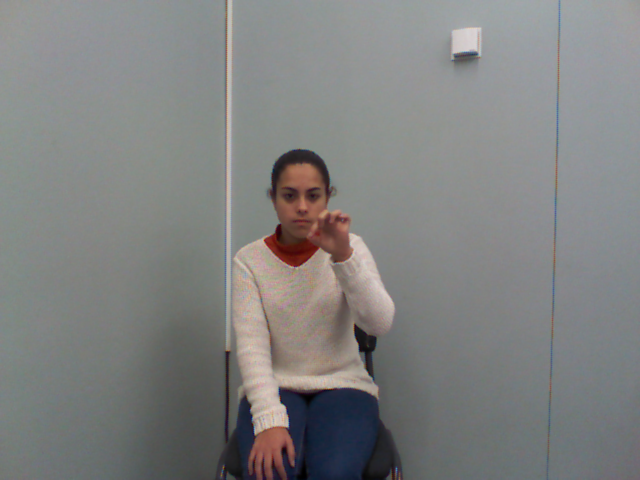
\includegraphics[interpolate=true, height=0.50\columnwidth]{ChapterFour/4_psl.png}};
            \spy on (0.04,0.05) in node [left] at (1.6,0.9);
        \end{tikzpicture}
    \end{minipage}
    \hspace{0.00mm}
    \begin{minipage}[t]{0.3\columnwidth}
        \begin{tikzpicture}[spy using outlines={circle,red,magnification=4,size=1.4cm, connect spies}]
            \node {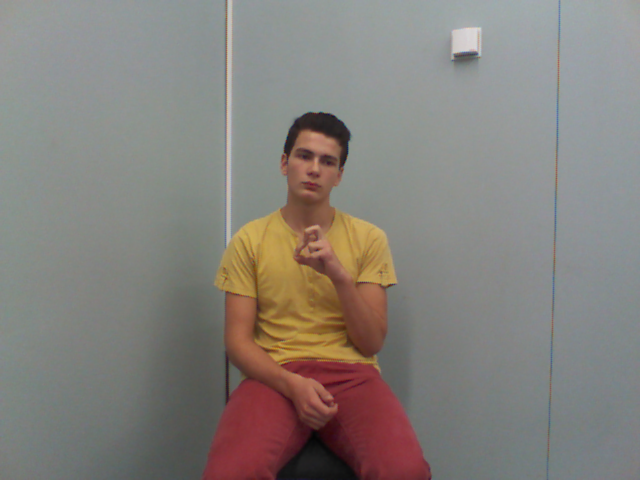
\includegraphics[interpolate=true, height=0.50\columnwidth]{ChapterFour/5_psl.png}};
            \spy on (0.001,-0.05) in node [left] at (1.6,0.9);
        \end{tikzpicture}
    \end{minipage}
    \hspace{0.00mm}
    \begin{minipage}[t]{0.3\columnwidth}
        \begin{tikzpicture}[spy using outlines={circle,red,magnification=4,size=1.4cm, connect spies}]
            \node {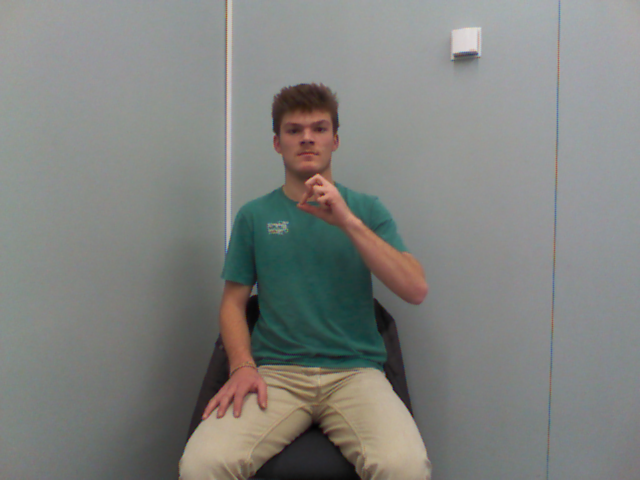
\includegraphics[interpolate=true, height=0.50\columnwidth]{ChapterFour/6_psl.png}};
            \spy on (0.02,0.17) in node [left] at (1.6,0.9);
        \end{tikzpicture}
    \end{minipage}
    \caption{Illustration of the inter-signer variability using some samples of the CorSiL database. The six signers are performing the sign ``eight" of the Portuguese sign language.}
    \label{fig:corsil}
\end{figure}

\subsubsection{Baselines}
In addition to the baselines used in \Secref{sec:adv_signer_inv_experiments} and to our previous model, we implemented two further models for comparison here:
\begin{itemize}
    \item DANN, by \citet{Ganin2015}, which we have already discussed extensively. The application of this method to our problem implied two main changes in the original method: i) the binary domain-classifier (source vs. target domain) was extended to $k$ classes (number of signers in the training data); ii) since our data is fully annotated (sign classes and signer identities are always available), training was performed in a fully supervised fashion.
    \item DTML, by \citet{Hu2016}, a reconstruction-based domain adaption algorithm. The implementation of this methodology for our particular task also implied the generalization of the original model from one single domain to $k$ source domains.
\end{itemize}

\subsubsection{Results and discussion}

\Tableref{tab:desire_jt_mklm_results} shows the classification accuracy of the proposed DeSIRe model and the two aforementioned baselines on Jochen-Triesch and MKLM datasets. For easy comparison, we replicate the results from \Tableref{tab:adv_signer_inv_results} for our adversarial model (\Secref{sec:adv_signer_inv}). The results for the remaining baselines are omitted since they are the same as before and inferior to those of our adversarial model.

\begin{table}[t]
    \centering
    \resizebox{\linewidth}{!}{
        \begin{tabular}{c|c c c|c c c}
            & \multicolumn{3}{c|}{Jochen Triesch} & \multicolumn{3}{c}{MKLM}\\
            & Uniform  Bg.      & Complex Bg.        & Both  & Avg. $\pm$ std.  & min         & max        \\ \hline
            DANN \cite{Ganin2015} & 98.13 & 83.75  & 93.33 & 94.30 \footnotesize{$\pm 2.49$} & 91.50 & 96.50 \\
            DTML \cite{Hu2016} & 98.75 & 85.63  & 94.38 & 94.10 \footnotesize{$\pm 3.84$} & 87.00 & 97.50 \\
            \hline
            Proposed adv.\ model (\Secref{sec:adv_signer_inv})       &      98.75     & 91.25
            &   96.25 &    94.80 \footnotesize{$\pm 3.53$}      &  89.50
            &  \textbf{100.00}    \\
            DeSIRe & \textbf{99.69} & \textbf{92.50} & \textbf{97.29} & \textbf{96.80} \footnotesize{$\pm 2.38$} & \textbf{93.00} & 99.00
    \end{tabular}}
    \caption{Classification accuracy (\%) of DeSIRe and baselines on Jochen-Triesch and MKLM datasets.}
    \label{tab:desire_jt_mklm_results}
\end{table}

A first observation is the superior performance of DeSIRe. It is also worth mentioning that our previous model for domain generalization outperformed DANN and DTML in most settings. Nevertheless, the proposed model achieved by far the best overall classification accuracy. Another interesting observation is the performance of DeSIRe against complex backgrounds, which even exceeds that of our previous model. These results demonstrate the robustness of the proposed model to inter-signer variability as well as its capability of dealing with the large intra-signer variability of this dataset. As previously explained in \Secref{sec:desire_loss}, the robustness to intra-signer variability is mostly due to the proposed sampling scheme of the sign repetition introduced to the decoder network, which enforces the learned latent representations to discard this type of variability. Another important reason that may explain the superiority of DeSIRe is the fact that this model aligns class-conditional distributions, rather than marginal ones. Since all signers have labeled data and, for these datasets, the marginal class distributions are balanced across signers, aligning marginal feature distributions is less problematic here than in the problem of domain adaptation. Anyway, the explicit alignment of conditional distributions is preferable since it promotes class clustering in the latent space.

The classification accuracy for sign classification in the CorSiL database is presented in \Tableref{tab:desire_corsil_results}. As the SI-PSL database contains a large number of sign classes (31), the results are presented in terms of top-1, top-3 and top-5 classification accuracy. As shown in the table, the proposed DeSIRe model outperformed both the implemented baselines and the state of the art domain adaption methods in all the three classification metrics. However, it should be noticed that, regardless of the employed methodology, the overall performance in this database is significantly below that obtained in the other two databases. These results attest to the difficulty of the classification task on the presented database and should encourage further research on signer-independent SLR.

\begin{table}[t]
    \centering
    \begin{tabular}{c|c c c}
            & Top-1  & Top-3 & Top-5 \\\hline
            DANN \cite{Ganin2015} & 48.66             & 75.54                    & 83.33           \\
            DTML \cite{Hu2016} & 39.25            & 68.01                    & 79.84            \\
            \hline
            CNN (baseline 1)                              & 45.97           & 74.73          & 85.75        \\
            CNN with triplet loss (baseline 2)            &  42.74          & 72.31          & 81.99       \\
            Proposed adv.\ model (\Secref{sec:adv_signer_inv}) & 49.13 & 76.01 & 85.19 \\
            DeSIRe         & \textbf{51.88}  & \textbf{76.61} & \textbf{87.90}        \\
    \end{tabular}
    \caption{Classification accuracy (\%) of DeSIRe and baselines on the CorSiL dataset.}
    \label{tab:desire_corsil_results}
\end{table}

Since DeSIRe is a rather complex model, with multiple loss terms and techniques to enhance its performance, we believe it is highly instructive to provide a more thorough analysis of its training behavior and further experimental results. Both are presented in Appendix~\ref{appendix:desire}. Specifically, we present a qualitative and quantitative analysis of the learned latent representations in Appendices \ref{sec:desire_tsne} and \ref{sec:desire_clusters}, respectively. We illustrate the interaction of the multiple loss terms in Appendix~\ref{sec:desire_training_behav}. A hyperparameter sensitivity analysis is conducted in Appendix~\ref{sec:desire_hyperparam}.

\section{Conclusion}
\label{sec:desire_conclusion}
This paper addresses the topic of signer-independent sign language recognition. To tackle this problem, we propose a novel end-to-end deep neural network along with a well-designed loss function that explicitly models signer-invariant latent representations from the data. Specifically, the proposed model is composed by two main modules: (i) a conditional variational autoencoder (CVAE), and (ii) a classifier. The purpose of the CVAE module is to learn latent representations of the input data, whose conditional posterior distribution, given the image and its sign label, is independent of the signer identity. During the training stage, the CVAE plays the role of a teacher model for the classifier, since the conditional posterior distribution over latent representations is used to regularize the hidden representations of the classifier. These signer-invariant hidden representations are then used for a robust signer-independent SLR recognition. Experimental results demonstrate the robustness of the proposed model to new test signers. The proposed model provides quite promising results, outperforming the implemented baseline methods and current state-of-the-art SLR and domain adaptation methods in different SLR databases. Extending the proposed DeSIRe model to dynamic signs (i.e.\ video) is an interesting direction for future work.

% Add others as needed


%-------------------------------------------------------------------------
%	THESIS CONTENT - APPENDICES
%-------------------------------------------------------------------------

\appendix % Cue to tell LaTeX that the following 'chapters' are Appendices

%%% -----------  ADD APPENDIX HERE ------------------ %%%

% Appendix Template

\chapter{SpaMHMM -- supplementary material} % Main appendix title

\label{appendix:spamhmm} % Change X to a consecutive letter; for referencing this appendix elsewhere, use \ref{AppendixX}

\section{Derivation of the EM learning algorithms for MHMM and SpaMHMM}

\subsection{EM for MHMM (\Algref{alg:mhmm})}
\label{sec:proof_em_noreg}
\Algref{alg:mhmm} follows straightforwardly from applying EM to the model defined by \twoeqrefs{eq:spamhmm_density}{eq:spamhmm_hmm} with the objective \plaineqref{eq:spamhmm_log_likelihood}. As explained in \secref{sec:background_em}, for table CPDs, the E-step consists in finding expected sufficient statistics $M(x, u)$ and $M(u)$, as defined in \twoeqrefs{eq:?}{eq:?} for each $(x, u) \in \mathrm{Val}(\rx,  \parents_\gG(\rx))$, where $\gG$ is the Bayesian network in \Figref{fig:spamhmm_bayesian_net}. Thus, in our setting, those equations yield:
\begingroup
\allowdisplaybreaks
\begin{align}
	&M(z,y) = \sum_{i=1}^{n} p(y, z \mid \vx_i, y_i) = \sum_{i=1}^{n} p(z \mid \vx_i, y_i) \1_{y_i=y}, \\
	&M(y) = \sum_{i=1}^{n} p(y \mid \vx_i, y_i) = \sum_{i=1}^{n} \1_{y_i=y}, \\
	&M(\rh^{(0)}=h, z) = \sum_{i=1}^{n} p(\rh^{(0)}=h, z \mid \vx_i, y_i) = \sum_{i=1}^{n} p(\rh^{(0)}=h \mid \vx_i, y_i, z) p(z \mid \vx_i, y_i) \nonumber\\
	&\hphantom{M(\rh^{(0)}=h,z)} = \sum_{i=1}^{n} p(\rh^{(0)}=h \mid \vx_i, y_i) p(z \mid \vx_i, y_i), \\
	&M(z) = \sum_{i=1}^{n} p(z \mid \vx_i, y_i), \\
	&M(\rh^{(t)}=h', \rh^{(t-1)}=h, z) = \sum_{i=1}^{n} p(\rh^{(t)}=h', \rh^{(t-1)}=h, z \mid \vx_i, y_i) \nonumber\\
	&\hphantom{M(\rh^{(t-1)}=h, } = \sum_{i=1}^{n} p(\rh^{(t)}=h' \mid \rh^{(t-1)}=h, \vx_i, z) p(\rh^{(t-1)}=h \mid \vx_i, z) p(z \mid \vx_i, y_i), \\
	&M(\rh^{(t-1)}=h, z) = \sum_{i=1}^{n} p(\rh^{(t-1)}=h, z \mid \vx_i, y_i) \nonumber\\
	&\hphantom{M(\rh^{(t-1)}=h, z)} = \sum_{i=1}^{n} p(\rh^{(t-1)}=h \mid \vx_i, z) p(z \mid \vx_i, y_i).
\end{align}
\endgroup
These equations allow us to compute the following updates in the M-step:
\begin{align}
	\evalpha^{(y)}_z = \frac{M(y,z)}{M(y)} \quad \text{and} \quad \evpi^{(z)}_h = \frac{M(\rh^{(0)}=h, z)}{M(z)}.
\end{align}
For the state transition matrices update, the same idea applies after summing over the sequence length:
\begin{equation}
	\emA^{(z)}_{h,h'} = \frac{\sum_{t=1}^T M(\rh^{(t)}=h', \rh^{(t-1)}=h, z)}{\sum_{t=1}^T M(\rh^{(t-1)}=h, z)}.
\end{equation}
Now, defining $n_y$, $\eta^{(z)}_i$, $\gamma^{(z)}_{i,h}(t)$, and $\xi^{(z)}_{i,h,h'}(t)$ as in \Algref{alg:mhmm}, the update formulas for $\evalpha^{(y)}_z$, $\evpi^{(z)}_h$, and $\emA^{(z)}_{h,h'}$ become as defined in that algorithm.

Deriving the update equations for the means and covariances of the Gaussian emission distributions is not so simple, since these are not table CPDs and therefore the procedure we have just used is no longer valid. Nonetheless, the desired equations can be obtained by explicitly maximizing the ELBO with respect to these parameters. As we have seen in \secref{sec:background_em},
\begin{equation}
	\label{eq:mhmm_elbo}
	\mathrm{ELBO} = \sum_{i=1}^{n} \E_{(\rvh_i,\rz_i) \sim q} \log p(\mX_i, \rvh_i, \rz_i \mid y_i; \Theta),
\end{equation}
where $q(\rvh_i,\rz_i) = p(\rvh_i, \rz_i \mid \vx_i, y_i; \Theta^{(-)})$, being $\Theta^{(-)}$ the set of current values for all parameters. We are solely interested in maximizing the ELBO with respect to the parameters $\vmu^{(z)}_h$ and $\vsigma^{(z)}_h$, so we can plug in the expression for the joint $p(\vx_i, \rvh_i, \rz_i \mid y_i; \Theta)$ and ignore all terms that do not depend on these parameters:
\begin{align}
	\label{eq:mhmm_elbo_gaussian_params}
	\mathrm{ELBO} &= \sum_{i=1}^n \sum_{\rvh_i, \rz_i} q(\rvh_i,\rz_i) \log \left[p(\rz_i \mid y_i) p(\rh^{(0)}_i \mid \rz_i) \prod_t p(\rh^{(t)}_i \mid \rh^{(t-1)}_i, \rz_i) p(\vx^{(t)}_i \mid \rh^{(t)}_i, \rz_i) \right] \nonumber\\
	&= \sum_{i=1}^n \sum_{\rh^{(t)}_i, \rz_i} \sum_{t=1}^{T_i} q(\rh^{(t)}_i, \rz_i) \log p(\vx^{(t)}_i \mid \rh^{(t)}_i, \rz_i) + \text{const}.
\end{align}
Now, all that remains is computing the gradient of the ELBO with respect to the parameters and solving for the critical points:
\begin{align}
&\nabla_{\vmu^{(z)}_h} \mathrm{ELBO} = \sum_{i=1}^n \sum_{t=1}^{T_i} \frac{q(\rh^{(t)}_i=h, z)}{p(\vx^{(t)}_i \mid \rh^{(t)}_i=h, z)} \nabla_{\vmu^{(z)}_h} p(\vx^{(t)}_i \mid \rh^{(t)}_i=h, z) \nonumber\\
&\hphantom{\nabla_{\vmu^{(z)}_h} \mathrm{ELBO}} = \sum_{i=1}^n  \sum_{t=1}^{T_i} q(\rh^{(t)}_i=h, z) \frac{\vx^{(t)}_i - \vmu^{(z)}_h}{{\vsigma^{(z)}_h}^2}, \\
&\nabla_{\vsigma^{(z)}_h} \mathrm{ELBO} = \sum_{i=1}^n \sum_{t=1}^{T_i} \frac{q(\rh^{(t)}_i=h, z)}{p(\vx^{(t)}_i \mid \rh^{(t)}_i=h, z)} \nabla_{\vsigma^{(z)}_h} p(\vx^{(t)}_i \mid \rh^{(t)}_i=h, z) \nonumber\\
&\hphantom{\nabla_{\vsigma^{(z)}_h} \mathrm{ELBO}} = \sum_{i=1}^n  \sum_{t=1}^{T_i} q(\rh^{(t)}_i=h, z) \left(\frac{(\vx^{(t)}_i - \vmu^{(z)}_h)^2}{{\vsigma^{(z)}_h}^3} - \frac{1}{\vsigma^{(z)}_h}\right),
\end{align}
where vector division and exponentiation should be interpreted as elementwise operations. Finally, solving for the critical points yields:
\begin{align}
&\vmu^{(z)}_h = \frac{\sum_{i=1}^n  \sum_{t=1}^{T_i} q(\rh^{(t)}_i=h, z) \vx^{(t)}_i}{\sum_{i=1}^n  \sum_{t=1}^{T_i} q(\rh^{(t)}_i=h, z)} \nonumber\\
&\hphantom{\vmu^{(z)}_h} = \frac{\sum_{i=1}^n p(z \mid \mX_i, y_i; \Theta^{(-)}) \sum_{t=1}^{T_i} p(\rh^{(t)}=h \mid \mX_i, z; \Theta^{(-)}) \vx^{(t)}_i}{\sum_{i=1}^n p(z \mid \mX_i, y_i; \Theta^{(-)}) \sum_{t=1}^{T_i} p(\rh^{(t)}=h \mid \mX_i, z; \Theta^{(-)})}, \\
&{\vsigma^{(z)}_h}^2 = \frac{\sum_{i=1}^n  \sum_{t=1}^{T_i} q(\rh^{(t)}_i=h, z) (\vx^{(t)}_i - \vmu^{(z)}_h)^2}{\sum_{i=1}^n  \sum_{t=1}^{T_i} q(\rh^{(t)}_i=h, z)} \nonumber\\
&\hphantom{{\vsigma^{(z)}_h}^2} = \frac{\sum_{i=1}^n p(z \mid \mX_i, y_i; \Theta^{(-)}) \sum_{t=1}^{T_i} p(\rh^{(t)}=h \mid \mX_i, z; \Theta^{(-)}) (\vx^{(t)}_i - \vmu^{(z)}_h)^2}{\sum_{i=1}^n p(z \mid \mX_i, y_i; \Theta^{(-)}) \sum_{t=1}^{T_i} p(\rh^{(t)}=h \mid \mX_i, z; \Theta^{(-)})}.
\end{align}
Again, the formulas in \Algref{alg:mhmm} follow by plugging $\eta^{(z)}_i$ and $\gamma^{(z)}_{i,h}(t)$ into the expressions above. $\quad \square$

\subsection{EM for SpaMHMM (\Algref{alg:spamhmm})}
\label{sec:proof_em_reg}
We start by showing that the E-step is unaffected by the regularization term in \eqref{eq:spamhmm_objective} and then we will derive the update equations for the M-step.

As is a common practice in EM and variational methods, let $q(\rz, \rvh)$ be an arbitrary distribution over the hidden variables of our model whose support is contained in the support of $p$. Then,
\begin{align}
	J_r(\Theta) &= \frac{1}{n}\sum_{i=1}^n \log \E_{(\rz_i, \rvh_i) \sim q} \left[ \frac{p(\mX_i \mid y_i; \Theta)}{q(\rz_i, \rvh_i)} \right] + \reg R(\gG; \Theta) \nonumber\\
	&\geq  \frac{1}{n}\sum_{i=1}^n \E_{(\rz_i, \rvh_i) \sim q} \log \left[ \frac{p(\mX_i \mid y_i; \Theta)}{q(\rz_i, \rvh_i)} \right] + \reg R(\gG; \Theta).
\end{align}
where the inequality is a direct result of Jensen's inequality and $R(\gG; \Theta)$ is our regularization term, as defined in \eqref{eq:spamhmm_objective}. We are therefore interested in maximizing this lower bound with respect to both $\Theta$ and $q$. Since $R(\gG; \Theta)$ does not depend on $q$, maximization with respect to this distribution while fixing $\Theta = \Theta^{(-)}$ yields $q(\rz_i, \rvh_i) = p(\rz_i, \rvh_i \mid \mX_i, y_i; \Theta^{(-)})$, as for the case of standard (i.e. unregularized) EM. Thus,
\begin{equation}
	J_r(\Theta) \geq \frac{1}{n} \mathrm{ELBO}(\Theta) + \lambda R(\gG; \Theta) + \text{const},
\end{equation}
where the ELBO takes the exact same form as in \eqref{eq:mhmm_elbo}. 

Now all that remains is the maximization of this lower bound with respect to $\Theta$. After noting that some parameters are constrained to sum up to 1, we could build the following Lagrangian and solve for the critical points:
\begin{align}
	L(\Theta, \Lambda) = & \frac{1}{n} \mathrm{ELBO}(\Theta) + \lambda R(\gG; \Theta) + \sum_{y=1}^k \mu_y\left(1 - ||\valpha^{(y)}||_{1}\right) \nonumber\\
	&+ \sum_{z=1}^m \sum_{h=1}^s \nu^{(z)}_h \left(1 - \sum_{h'=1}^s \emA^{(z)}_{h,h'}\right) 
	+ \sum_{z=1}^m \varrho_z \left(1 - ||\vpi_z||_{1}\right),
\end{align}
where $\Lambda \triangleq \bigcup_{h,y,z} \{\mu_y, \nu^{(z)}_h, \varrho_z\}$ is the set of all Lagrange multipliers. Since $R(\gG; \Theta)$ only depends on the mixture coefficients $\valpha^{(y)}$, the update equations for all parameters except those are exactly the same as in \Algref{alg:mhmm}. 

Unfortunately, setting $\nabla L = 0$ yields a system of equations that is non-linear in $\valpha^{(y)}$ and no analytical solution can be found. However, we can resort to the reparametrization defined in \eqref{eq:spamhmm_normalization} and update the new parameters $\vbeta^{(y)}$ by performing gradient ascent over the unconstrained lower bound. Thus, computing the required gradient concludes the derivation of the algorithm.

Now we only care about the dependency of the ELBO on the mixture coefficients, so, following the same idea as in \eqref{eq:mhmm_elbo_gaussian_params}, we can write:
\begin{align}
	\mathrm{ELBO} &= \frac{1}{n}\sum_{i=1}^n \sum_{\rz_i} q(\rz_i) \log p(\rz_i \mid y_i) + \text{const} \nonumber\\
	&= \frac{1}{n}\sum_{i=1}^n \sum_{z=1}^m q(z) \log \evalpha^{(y_i)}_{z} + \text{const},
\end{align}
and therefore,
\begin{equation}
	\frac{\partial \mathrm{ELBO}}{\partial \evalpha^{(y)}_{z}} = \frac{1}{n}\sum_{i=1}^n \frac{q(z)}{\evalpha^{(y)}_{z}} \1_{y_i=y}, \quad
	\frac{\partial R}{\partial \evalpha^{(y)}_{z}} = \frac{1}{2}\sum_{\substack{y'=1,\\y'\neq y}}^{k} \emG_{y,y'} \evalpha^{(y')}_{z}.
\end{equation}
Finally, by the chain rule,
\begin{align}
	&\frac{\partial \mathrm{ELBO}}{\partial \evbeta^{(y)}_{z}} = \sum_{z'=1}^{m} \frac{\partial \mathrm{ELBO}}{\partial \evalpha^{(y)}_{z'}} \frac{\partial \evalpha^{(y)}_{z'}}{\partial \evbeta^{(y)}_{z}} \nonumber\\
	&\hphantom{\frac{\partial \mathrm{ELBO}}{\partial \evbeta^{(y)}_{z}}} = \frac{1}{n} \sum_{i=1}^n \left(q(z) - \evalpha^{(y)}_{z}\right) \1_{y_i = y \wedge \evbeta^{(y)}_{z} > 0} \nonumber\\
	&\hphantom{\frac{\partial \mathrm{ELBO}}{\partial \evbeta^{(y)}_{z}}} = \frac{1}{n} \sum_{i=1}^n \left(p(z \mid \mX_i, y_i; \Theta^{(-)}) - \evalpha^{(y)}_{z}\right) \1_{y_i = y \wedge \evbeta^{(y)}_{z} > 0}, \\
	&\frac{\partial R}{\partial \evbeta^{(y)}_{z}} = \sum_{z'=1}^{m} \frac{\partial R}{\partial \evalpha^{(y)}_{z'}} \frac{\partial \evalpha^{(y)}_{z'}}{\partial \evbeta^{(y)}_{z}} \nonumber\\
	&\hphantom{\frac{\partial R}{\partial \evbeta^{(y)}_{z}}} = \evalpha^{(y)}_{z} \sum_{\substack{y'=1,\\y'\neq y}}^{k} \emG_{y,y'} \left(\evalpha^{(y')}_{z} - {\valpha^{(y')}} \transp \valpha^{(y)} \right) \1_{\evbeta^{(y)}_{z} > 0},
\end{align}
and considering $\psi^{(y)}_{z}$, $\omega^{(y)}_{z}$, and $\delta^{(y)}_z$ as defined in \Algref{alg:spamhmm} and the gradient ascent update rule the formulas follow. $\quad \square$

\section{Posterior distribution of observations}
\label{sec:posterior_proof}
In this section, we show how to obtain the posterior distribution $p(\rmX \mid \mX_\text{pref}, y)$ of sequences $\rmX \triangleq \left(\rvx^{(1)}, ...,\rvx^{(t)}\right)$ given an observed prefix sequence $\mX_\text{pref} \triangleq \left(\vx^{(-t_\text{pref}+1)}, ...,\vx^{(0)}\right)$, both coming from the graph node $y$. We start by writing this posterior as a marginalization with respect to the latent variable $\rz$:
\begin{align}
\label{mhmm_posterior}
p(\rmX \mid \mX_\text{pref}, y) &= \sum_{\rz} p(\rmX, \rz \mid \mX_\text{pref}, y)\nonumber\\
&= \sum_{\rz} p(\rmX \mid \mX_\text{pref}, y, \rz) p(\rz \mid \mX_\text{pref}, y) \nonumber\\
&= \sum_{\rz} p(\rmX \mid \mX_\text{pref}, \rz) p(\rz \mid \mX_\text{pref}, y),
\end{align}
where the last equality follows from the fact that the observations $\rmX$ are conditionally independent of the graph node $\ry$ given the latent variable $\rz$. The posterior $p(\rz \mid \mX_\text{pref}, y)$ may be obtained as done in \Algref{alg:mhmm}:
\begin{equation}
p(\rz \mid \mX_\text{pref}, y) \propto p(\mX_\text{pref} \mid \rz)p(\rz \mid y).
\end{equation}
We now focus on the computation of $p(\rmX \mid \mX_\text{pref}, \rz)$. Let $\rvh_\text{pref} \triangleq \left(\rh^{(-t_\text{pref}+1)}, ...,\rh^{(-1)}\right)$ and $\rvh \triangleq \left(\rh^{(0)}, ...,\rh^{(t)}\right)$, then:
\begin{align}
p(\rmX \mid \mX_\text{pref}, \rz) &= \sum_{\rvh_\text{pref}, \rvh} p(\rmX, \rvh_\text{pref}, \rvh \mid \mX_\text{pref}, \rz) \nonumber\\
&= \sum_{\rvh_\text{pref}, \rvh} p(\rmX \mid \rvh_\text{pref}, \rvh, \mX_\text{pref}, \rz) p(\rvh_\text{pref}, \rvh \mid \mX_\text{pref}, \rz) \nonumber\\
&= \sum_{\rvh_\text{pref}, \rvh} p(\rmX \mid \rvh, \rz) p(\rvh_\text{pref} \mid \rvh, \mX_\text{pref}, \rz) p(\rvh \mid \mX_\text{pref}, \rz) \nonumber\\
&= \sum_{\rvh} p(\rmX \mid \rvh, \rz) p(\rvh \mid \mX_\text{pref}, \rz) \nonumber\\
&= \sum_{\rvh} p(\rh^{(0)} \mid \mX_\text{pref}, \rz) \prod_{\tau=1}^{t} p(\rh^{(\tau)} \mid \rh^{(\tau-1)}, \rz) p(\rvx^{(\tau)} \mid \rh^{(\tau)}, \rz),
\end{align}
where we have used the independence assumptions that characterize the HMM. Here, the initial state posteriors $p(\rh^{(0)} \mid \mX_\text{pref}, \rz)$ are actually the final state posteriors for the sequence $\mX_\text{pref}$ for each HMM in the mixture, so they can also be computed as indicated \Algref{alg:mhmm}.

Thus, we conclude that inference in the posterior model $p(\rmX \mid \mX_\text{pref}, y)$ corresponds to inference in a (Spa)MHMM where the original mixture coefficients and initial state probabilites are replaced with their respective posteriors, $p(\rz \mid \mX_\text{pref}, y)$ and $p(\rh^{(0)} \mid \mX_\text{pref}, \rz)$. All remaining parameters are unchanged.
% Appendix Template

\chapter{Tackling unsupervised domain adaptation with optimism and consistency -- supplementary material} % Main appendix title
\chaptermark{Tackling UDA with optimism and consistency -- supp. material}

\label{appendix:modafm} % Change X to a consecutive letter; for referencing this appendix elsewhere, use \ref{AppendixX}

\section{Proof of Theorem \ref{thm:target_risk_bound}}
\label{sec:thm_proof}

The presented bound is an immediate consequence of two theorems of \cite{BenDavid2010, Blitzer2008}, which we present here as lemmas:

\begin{lemma}
	\label{lemma:bound_mixture}
	(Lemma 4 from \citet{Blitzer2008}) Let $\gH$ be a hypothesis class with VC-dimension $d$. For each $j \in \{1,2,...,k\}$, consider a labeled set of $n/k$ samples drawn from the source domain $\gS_j$. For any $h \in \gH$ and any $\valpha \in \Delta$, with probability at least $1-\delta$ over the choice of samples,
	
	\begin{equation}
	|\widehat{\epsilon}_\valpha(h) - \epsilon_\valpha(h)| \leq 2\sqrt{\frac{k}{n} \left(2d\log(2(n+1)) + \log \frac{4}{\delta}\right) \sum_{j=1}^k \evalpha_j^2}.
	\end{equation}
\end{lemma}

\begin{lemma}
	\label{lemma:bound_single_source}
	(Theorem 2 from \citet{BenDavid2010}) Let $\gH$ be a hypothesis class with VC-dimension $d$. Consider $n$ unlabeled samples drawn from each of the two domains $\gS$ (source) and $\gT$ (target). Then, for every $h \in \gH$, with probability at least $1-\delta$ over the choice of samples,
	
	\begin{equation}
	\epsilon_\gT(h) \leq \epsilon_\gS(h) + \frac{1}{2} \widehat{d}_{\gH \Delta \gH}(\gS, \gT) + 2\sqrt{\frac{1}{n} \left( 2d\log(2n) + \log \frac{2}{\delta} \right)} + \lambda,
	\end{equation}    
	where $\lambda = \min_{h \in \gH} \epsilon_\gS(h) + \epsilon_\gT(h)$.
\end{lemma}

Proving our result is now straightforward. We can apply Lemma \ref{lemma:bound_single_source} taking $\gS_\valpha$ as the source domain. Note that $\epsilon_{S_\valpha}(h) = \sum_{j=1}^k \evalpha_j \epsilon_{S_j}(h)$ for any $h \in \gH$, and therefore $\lambda_\valpha = \min_{h \in \gH}\, \sum_{j=1}^k \evalpha_j\epsilon_{\gS_j}(h) + \epsilon_{\gT}(h)$. Combining the obtained bound with Lemma \ref{lemma:bound_mixture} through the union bound yields the desired result. $\square$

\section{Model overview}
\label{sec:model_overview}

\tikzset{every picture/.style={line width=0.75pt}} %set default line width to 0.75pt      
\begin{figure}[h!]
	\centering
	\hspace*{-0.30in}
	\scalebox{.69}{\begin{tikzpicture}[x=0.75pt,y=0.75pt,yscale=-1,xscale=1]
%uncomment if require: \path (0,392); %set diagram left start at 0, and has height of 392

%Shape: Rectangle [id:dp3324670647624888]
\draw  [draw opacity=0][fill={rgb, 255:red, 245; green, 166; blue, 35 }  ,fill opacity=0.27 ][dash pattern={on 4.5pt off 4.5pt}] (404.28,161.03) -- (463.28,161.03) -- (463.28,234.03) -- (404.28,234.03) -- cycle ;
%Shape: Rectangle [id:dp8725257093919785]
\draw  [draw opacity=0][fill={rgb, 255:red, 124; green, 163; blue, 233 }  ,fill opacity=0.27 ][dash pattern={on 4.5pt off 4.5pt}] (404.31,10.33) -- (493.98,10.33) -- (493.98,122.69) -- (404.31,122.69) -- cycle ;
%Shape: Rectangle [id:dp7324245449252831]
\draw  [draw opacity=0][fill={rgb, 255:red, 255; green, 199; blue, 199 }  ,fill opacity=0.46 ][dash pattern={on 4.5pt off 4.5pt}] (477.64,147) -- (567.31,147) -- (567.31,259.36) -- (477.64,259.36) -- cycle ;
%Shape: Rectangle [id:dp6062966359758601]
\draw  [draw opacity=0][fill={rgb, 255:red, 245; green, 166; blue, 35 }  ,fill opacity=0.27 ][dash pattern={on 4.5pt off 4.5pt}] (404.28,273.03) -- (463.28,273.03) -- (463.28,346.03) -- (404.28,346.03) -- cycle ;
%Shape: Rectangle [id:dp630018718197102]
\draw  [draw opacity=0][fill={rgb, 255:red, 139; green, 87; blue, 42 }  ,fill opacity=0.27 ][dash pattern={on 4.5pt off 4.5pt}] (299.28,273.36) -- (358.28,273.36) -- (358.28,346.36) -- (299.28,346.36) -- cycle ;
%Shape: Rectangle [id:dp6477196776803296]
\draw  [draw opacity=0][fill={rgb, 255:red, 226; green, 223; blue, 223 }  ,fill opacity=0.46 ][dash pattern={on 4.5pt off 4.5pt}] (234.52,57.63) -- (337.85,57.63) -- (337.85,209.3) -- (234.52,209.3) -- cycle ;
%Shape: Rectangle [id:dp8132847865870008]
\draw  [draw opacity=0][fill={rgb, 255:red, 184; green, 233; blue, 134 }  ,fill opacity=0.46 ][dash pattern={on 4.5pt off 4.5pt}] (74.45,194.3) -- (165.45,194.3) -- (165.45,234) -- (74.45,234) -- cycle ;
%Shape: Trapezoid [id:dp5704780838781891]
\draw   (266.83,91.34) -- (303.92,102.47) -- (303.92,163) -- (266.83,174.13) -- cycle ;
%Straight Lines [id:da9939618725818478]
\draw    (214.2,133.63) -- (262.8,133.63) ;
\draw [shift={(265.8,133.68)}, rotate = 180] [fill={rgb, 255:red, 0; green, 0; blue, 0 }  ][line width=0.08]  [draw opacity=0] (8.93,-4.29) -- (0,0) -- (8.93,4.29) -- cycle    ;
%Straight Lines [id:da34915626003255906]
\draw    (304,133.5) -- (380.79,133.5) ;
%Shape: Rectangle [id:dp3470774888051449]
\draw   (466.18,40.03) -- (466.18,85.38) -- (433.01,85.38) -- (433.01,40.03) -- cycle ;
%Straight Lines [id:da8554977587366552]
\draw    (465.98,62.76) -- (508.94,62.76) ;
\draw [shift={(511.94,62.83)}, rotate = 180] [fill={rgb, 255:red, 0; green, 0; blue, 0 }  ][line width=0.08]  [draw opacity=0] (8.93,-4.29) -- (0,0) -- (8.93,4.29) -- cycle    ;
%Straight Lines [id:da8625467456853719]
\draw    (380.79,133.35) -- (380.79,62.72) -- (430,62.72) ;
\draw [shift={(433,63)}, rotate = 180] [fill={rgb, 255:red, 0; green, 0; blue, 0 }  ][line width=0.08]  [draw opacity=0] (8.93,-4.29) -- (0,0) -- (8.93,4.29) -- cycle    ;
%Straight Lines [id:da6458708868066732]
\draw    (380.79,133.35) -- (380.79,204.61) -- (427.1,204.61) ;
\draw [shift={(430.1,204.98)}, rotate = 180] [fill={rgb, 255:red, 0; green, 0; blue, 0 }  ][line width=0.08]  [draw opacity=0] (8.93,-4.29) -- (0,0) -- (8.93,4.29) -- cycle    ;
%Shape: Rectangle [id:dp6014736791644808]
\draw   (155.01,224.06) -- (84.94,224.06) -- (84.94,204.67) -- (154.97,204.67) -- cycle ;
%Straight Lines [id:da5827721753553903]
\draw    (139,144) -- (139,202) ;
\draw [shift={(138.5,205)}, rotate = 270] [fill={rgb, 255:red, 0; green, 0; blue, 0 }  ][line width=0.08]  [draw opacity=0] (8.93,-4.29) -- (0,0) -- (8.93,4.29) -- cycle    ;
%Straight Lines [id:da6247068144527612]
\draw    (94.5,176) -- (94.5,201) ;
\draw [shift={(94.5,204)}, rotate = 270] [fill={rgb, 255:red, 0; green, 0; blue, 0 }  ][line width=0.08]  [draw opacity=0] (8.93,-4.29) -- (0,0) -- (8.93,4.29) -- cycle    ;
%Straight Lines [id:da8673602947674643]
\draw    (119.5,224) -- (119.5,251.5) ;
\draw [shift={(120,254.5)}, rotate = 270] [fill={rgb, 255:red, 0; green, 0; blue, 0 }  ][line width=0.08]  [draw opacity=0] (8.93,-4.29) -- (0,0) -- (8.93,4.29) -- cycle    ;
%Shape: Circle [id:dp6579495722327415]
\draw   (208.77,133.63) .. controls (208.77,132.13) and (209.99,130.92) .. (211.49,130.92) .. controls (212.98,130.92) and (214.2,132.13) .. (214.2,133.63) .. controls (214.2,135.13) and (212.98,136.35) .. (211.49,136.35) .. controls (209.99,136.35) and (208.77,135.13) .. (208.77,133.63) -- cycle ;
%Shape: Circle [id:dp10338753824617153]
\draw   (183.69,35.97) .. controls (183.69,34.47) and (184.9,33.25) .. (186.4,33.25) .. controls (187.9,33.25) and (189.11,34.47) .. (189.11,35.97) .. controls (189.11,37.47) and (187.9,38.68) .. (186.4,38.68) .. controls (184.9,38.68) and (183.69,37.47) .. (183.69,35.97) -- cycle ;
%Straight Lines [id:da16206023412720572]
\draw    (166.57,132.97) -- (184.4,132.97) ;
%Shape: Circle [id:dp05237936348106498]
\draw   (184.4,132.97) .. controls (184.4,131.47) and (185.62,130.25) .. (187.11,130.25) .. controls (188.61,130.25) and (189.83,131.47) .. (189.83,132.97) .. controls (189.83,134.47) and (188.61,135.68) .. (187.11,135.68) .. controls (185.62,135.68) and (184.4,134.47) .. (184.4,132.97) -- cycle ;
%Straight Lines [id:da7376138719283598]
\draw    (158.2,268.97) -- (184.4,268.97) ;
%Shape: Circle [id:dp3094036765477939]
\draw   (184.4,268.97) .. controls (184.4,267.47) and (185.62,266.25) .. (187.11,266.25) .. controls (188.61,266.25) and (189.83,267.47) .. (189.83,268.97) .. controls (189.83,270.47) and (188.61,271.68) .. (187.11,271.68) .. controls (185.62,271.68) and (184.4,270.47) .. (184.4,268.97) -- cycle ;
%Straight Lines [id:da3613846415308859]
\draw  [dash pattern={on 0.84pt off 2.51pt}]  (189.11,35.97) -- (207.97,132.97) ;
%Straight Lines [id:da3089522793482711]
\draw  [dash pattern={on 0.84pt off 2.51pt}]  (207.97,132.97) -- (189.83,132.97) ;
%Straight Lines [id:da4153933780669705]
\draw  [dash pattern={on 0.84pt off 2.51pt}]  (187.11,266.25) -- (208.77,133.63) ;
%Shape: Rectangle [id:dp5754001882772488]
\draw   (540.18,181.03) -- (540.18,226.38) -- (507.01,226.38) -- (507.01,181.03) -- cycle ;
%Shape: Rectangle [id:dp7123673461660205]
\draw   (440.73,182.36) -- (440.73,225.07) -- (429.39,225.07) -- (429.39,182.36) -- cycle ;
%Straight Lines [id:da6347532395825457]
\draw    (441.2,204.98) -- (504.3,204.98) ;
\draw [shift={(507.3,204.98)}, rotate = 540] [fill={rgb, 255:red, 0; green, 0; blue, 0 }  ][line width=0.08]  [draw opacity=0] (8.93,-4.29) -- (0,0) -- (8.93,4.29) -- cycle    ;
%Shape: Circle [id:dp6082756784936818]
\draw   (511.94,62.83) .. controls (511.94,61.34) and (513.16,60.12) .. (514.66,60.12) .. controls (516.16,60.12) and (517.37,61.34) .. (517.37,62.83) .. controls (517.37,64.33) and (516.16,65.55) .. (514.66,65.55) .. controls (513.16,65.55) and (511.94,64.33) .. (511.94,62.83) -- cycle ;
%Shape: Circle [id:dp4428999659320625]
\draw   (533.5,27.95) .. controls (533.5,26.45) and (534.71,25.23) .. (536.21,25.23) .. controls (537.71,25.23) and (538.93,26.45) .. (538.93,27.95) .. controls (538.93,29.44) and (537.71,30.66) .. (536.21,30.66) .. controls (534.71,30.66) and (533.5,29.44) .. (533.5,27.95) -- cycle ;
%Shape: Circle [id:dp8670498891603877]
\draw   (533.61,62.83) .. controls (533.61,61.34) and (534.82,60.12) .. (536.32,60.12) .. controls (537.82,60.12) and (539.04,61.34) .. (539.04,62.83) .. controls (539.04,64.33) and (537.82,65.55) .. (536.32,65.55) .. controls (534.82,65.55) and (533.61,64.33) .. (533.61,62.83) -- cycle ;
%Shape: Circle [id:dp6677450010623003]
\draw   (534.16,99.61) .. controls (534.16,98.11) and (535.38,96.9) .. (536.88,96.9) .. controls (538.38,96.9) and (539.59,98.11) .. (539.59,99.61) .. controls (539.59,101.11) and (538.38,102.33) .. (536.88,102.33) .. controls (535.38,102.33) and (534.16,101.11) .. (534.16,99.61) -- cycle ;
%Straight Lines [id:da01358818166711151]
\draw    (538.93,27.95) -- (571.11,27.95) ;
\draw [shift={(574.11,28.17)}, rotate = 180] [fill={rgb, 255:red, 0; green, 0; blue, 0 }  ][line width=0.08]  [draw opacity=0] (8.93,-4.29) -- (0,0) -- (8.93,4.29) -- cycle    ;
%Straight Lines [id:da6660202702118951]
\draw    (539.04,63.04) -- (571.22,63.04) ;
\draw [shift={(574.22,63.06)}, rotate = 180] [fill={rgb, 255:red, 0; green, 0; blue, 0 }  ][line width=0.08]  [draw opacity=0] (8.93,-4.29) -- (0,0) -- (8.93,4.29) -- cycle    ;
%Straight Lines [id:da06989855647404064]
\draw    (539.59,99.61) -- (571.78,99.61) ;
\draw [shift={(574.78,99.83)}, rotate = 180] [fill={rgb, 255:red, 0; green, 0; blue, 0 }  ][line width=0.08]  [draw opacity=0] (8.93,-4.29) -- (0,0) -- (8.93,4.29) -- cycle    ;
%Straight Lines [id:da37283517620059836]
\draw  [dash pattern={on 0.84pt off 2.51pt}]  (517.37,62.83) -- (533.5,27.95) ;
%Straight Lines [id:da5766114105445679]
\draw  [dash pattern={on 0.84pt off 2.51pt}]  (517.37,62.83) -- (533.61,62.83) ;
%Straight Lines [id:da8288863342105754]
\draw  [dash pattern={on 0.84pt off 2.51pt}]  (517.37,65.83) -- (534.16,99.61) ;
%Straight Lines [id:da2535799757628039]
\draw    (540.42,204.86) -- (578.75,204.83) ;
\draw [shift={(581.75,204.83)}, rotate = 540] [fill={rgb, 255:red, 0; green, 0; blue, 0 }  ][line width=0.08]  [draw opacity=0] (8.93,-4.29) -- (0,0) -- (8.93,4.29) -- cycle    ;
%Shape: Circle [id:dp046803690942768705]
\draw   (581.75,204.83) .. controls (581.75,203.33) and (582.96,202.12) .. (584.46,202.12) .. controls (585.96,202.12) and (587.18,203.33) .. (587.18,204.83) .. controls (587.18,206.33) and (585.96,207.54) .. (584.46,207.54) .. controls (582.96,207.54) and (581.75,206.33) .. (581.75,204.83) -- cycle ;
%Shape: Circle [id:dp41016927833886907]
\draw   (603.5,167.95) .. controls (603.5,166.45) and (604.71,165.23) .. (606.21,165.23) .. controls (607.71,165.23) and (608.93,166.45) .. (608.93,167.95) .. controls (608.93,169.44) and (607.71,170.66) .. (606.21,170.66) .. controls (604.71,170.66) and (603.5,169.44) .. (603.5,167.95) -- cycle ;
%Straight Lines [id:da09506613547421505]
\draw    (608.93,168.15) -- (641.11,168.15) ;
\draw [shift={(644.11,168.17)}, rotate = 180] [fill={rgb, 255:red, 0; green, 0; blue, 0 }  ][line width=0.08]  [draw opacity=0] (8.93,-4.29) -- (0,0) -- (8.93,4.29) -- cycle    ;
%Straight Lines [id:da8022228162896732]
\draw  [dash pattern={on 0.84pt off 2.51pt}]  (587.37,202.83) -- (603.5,167.95) ;
%Shape: Circle [id:dp4538983623578463]
\draw   (602.81,204.43) .. controls (602.81,202.94) and (604.02,201.72) .. (605.52,201.72) .. controls (607.02,201.72) and (608.24,202.94) .. (608.24,204.43) .. controls (608.24,205.93) and (607.02,207.15) .. (605.52,207.15) .. controls (604.02,207.15) and (602.81,205.93) .. (602.81,204.43) -- cycle ;
%Straight Lines [id:da16194011976448786]
\draw    (608.24,204.64) -- (640.42,204.64) ;
\draw [shift={(643.42,204.66)}, rotate = 180] [fill={rgb, 255:red, 0; green, 0; blue, 0 }  ][line width=0.08]  [draw opacity=0] (8.93,-4.29) -- (0,0) -- (8.93,4.29) -- cycle    ;
%Straight Lines [id:da5107264369592]
\draw  [dash pattern={on 0.84pt off 2.51pt}]  (586.57,204.43) -- (602.81,204.43) ;
%Shape: Rectangle [id:dp3024311812148579]
\draw   (440.73,294.36) -- (440.73,337.07) -- (429.39,337.07) -- (429.39,294.36) -- cycle ;
%Straight Lines [id:da10062012888191751]
\draw    (441.2,316.98) -- (479.74,316.98) ;
\draw [shift={(482.74,317.28)}, rotate = 180] [fill={rgb, 255:red, 0; green, 0; blue, 0 }  ][line width=0.08]  [draw opacity=0] (8.93,-4.29) -- (0,0) -- (8.93,4.29) -- cycle    ;
%Straight Lines [id:da8589281888606779]
\draw [color={rgb, 255:red, 208; green, 2; blue, 27 }  ,draw opacity=1 ] [dash pattern={on 4.5pt off 4.5pt}]  (632.56,60.88) -- (666.27,60.97) ;
\draw [shift={(669.27,60.98)}, rotate = 180] [fill={rgb, 255:red, 208; green, 2; blue, 27 }  ,fill opacity=1 ][line width=0.08]  [draw opacity=0] (8.93,-4.29) -- (0,0) -- (8.93,4.29) -- cycle    ;
%Straight Lines [id:da2768876954063071]
\draw [color={rgb, 255:red, 208; green, 2; blue, 27 }  ,draw opacity=1 ] [dash pattern={on 4.5pt off 4.5pt}]  (590.06,100.38) -- (693.48,100.03) ;
%Rounded Rect [id:dp8632849648308387]
\draw  [color={rgb, 255:red, 208; green, 2; blue, 27 }  ,draw opacity=1 ][dash pattern={on 4.5pt off 4.5pt}] (668.66,51.06) .. controls (668.66,48.59) and (670.67,46.58) .. (673.14,46.58) -- (709.59,46.58) .. controls (712.06,46.58) and (714.07,48.59) .. (714.07,51.06) -- (714.07,64.5) .. controls (714.07,66.98) and (712.06,68.98) .. (709.59,68.98) -- (673.14,68.98) .. controls (670.67,68.98) and (668.66,66.98) .. (668.66,64.5) -- cycle ;
%Straight Lines [id:da5420395815668599]
\draw [color={rgb, 255:red, 206; green, 2; blue, 27 }  ,draw opacity=1 ] [dash pattern={on 4.5pt off 4.5pt}]  (693.5,73.5) -- (693.48,100.03) ;
\draw [shift={(693.5,70.5)}, rotate = 90] [fill={rgb, 255:red, 206; green, 2; blue, 27 }  ,fill opacity=1 ][line width=0.08]  [draw opacity=0] (8.93,-4.29) -- (0,0) -- (8.93,4.29) -- cycle    ;
%Straight Lines [id:da7608878923801714]
\draw [color={rgb, 255:red, 208; green, 2; blue, 27 }  ,draw opacity=1 ] [dash pattern={on 4.5pt off 4.5pt}]  (634.3,27.66) -- (772.89,28.16) ;
\draw [shift={(775.89,28.17)}, rotate = 180] [fill={rgb, 255:red, 208; green, 2; blue, 27 }  ,fill opacity=1 ][line width=0.08]  [draw opacity=0] (8.93,-4.29) -- (0,0) -- (8.93,4.29) -- cycle    ;
%Shape: Rectangle [id:dp3006596095680114]
\draw   (334.73,294.69) -- (334.73,337.4) -- (323.39,337.4) -- (323.39,294.69) -- cycle ;
%Straight Lines [id:da3160571047315086]
\draw    (334.8,317.7) -- (426.11,317.7) ;
\draw [shift={(429.11,317.28)}, rotate = 540] [fill={rgb, 255:red, 0; green, 0; blue, 0 }  ][line width=0.08]  [draw opacity=0] (8.93,-4.29) -- (0,0) -- (8.93,4.29) -- cycle    ;
%Shape: Circle [id:dp7194955012675206]
\draw  [fill={rgb, 255:red, 0; green, 0; blue, 0 }  ,fill opacity=1 ] (377.44,317.3) .. controls (377.44,315.8) and (378.66,314.58) .. (380.16,314.58) .. controls (381.65,314.58) and (382.87,315.8) .. (382.87,317.3) .. controls (382.87,318.8) and (381.65,320.01) .. (380.16,320.01) .. controls (378.66,320.01) and (377.44,318.8) .. (377.44,317.3) -- cycle ;
%Straight Lines [id:da7991153199949488]
\draw    (280.11,317.28) -- (319.01,317.28) ;
\draw [shift={(322.01,317.64)}, rotate = 180] [fill={rgb, 255:red, 0; green, 0; blue, 0 }  ][line width=0.08]  [draw opacity=0] (8.93,-4.29) -- (0,0) -- (8.93,4.29) -- cycle    ;
%Straight Lines [id:da8934806393385226]
\draw [color={rgb, 255:red, 208; green, 2; blue, 27 }  ,draw opacity=1 ] [dash pattern={on 4.5pt off 4.5pt}]  (543.03,316.76) -- (661.93,316.65) ;
\draw [shift={(664.93,316.65)}, rotate = 540] [fill={rgb, 255:red, 208; green, 2; blue, 27 }  ,fill opacity=1 ][line width=0.08]  [draw opacity=0] (8.93,-4.29) -- (0,0) -- (8.93,4.29) -- cycle    ;
%Straight Lines [id:da8739773170593568]
\draw [color={rgb, 255:red, 206; green, 2; blue, 27 }  ,draw opacity=1 ] [dash pattern={on 4.5pt off 4.5pt}]  (690.64,214.5) -- (689.93,304.29) ;
\draw [shift={(689.9,307.29)}, rotate = 270] [fill={rgb, 255:red, 206; green, 2; blue, 27 }  ,fill opacity=1 ][line width=0.08]  [draw opacity=0] (8.93,-4.29) -- (0,0) -- (8.93,4.29) -- cycle    ;
%Straight Lines [id:da9433693688601523]
\draw [color={rgb, 255:red, 208; green, 2; blue, 27 }  ,draw opacity=1 ] [dash pattern={on 4.5pt off 4.5pt}]  (730.46,167.9) -- (760.48,168.14) ;
%Straight Lines [id:da39470738648267667]
\draw [color={rgb, 255:red, 206; green, 2; blue, 27 }  ,draw opacity=1 ] [dash pattern={on 4.5pt off 4.5pt}]  (760.48,168.14) -- (759.33,315.95) ;
%Straight Lines [id:da39924566327442346]
\draw [color={rgb, 255:red, 208; green, 2; blue, 27 }  ,draw opacity=1 ] [dash pattern={on 4.5pt off 4.5pt}]  (713.18,315.9) -- (759.33,315.95) ;
\draw [shift={(710.18,315.9)}, rotate = 0.06] [fill={rgb, 255:red, 208; green, 2; blue, 27 }  ,fill opacity=1 ][line width=0.08]  [draw opacity=0] (8.93,-4.29) -- (0,0) -- (8.93,4.29) -- cycle    ;
%Straight Lines [id:da9228463793017965]
\draw [color={rgb, 255:red, 206; green, 2; blue, 27 }  ,draw opacity=1 ] [dash pattern={on 4.5pt off 4.5pt}]  (380.16,321.9) -- (380,370.51) ;
%Straight Lines [id:da6355384414978655]
\draw [color={rgb, 255:red, 208; green, 2; blue, 27 }  ,draw opacity=1 ] [dash pattern={on 4.5pt off 4.5pt}]  (383.03,370.26) -- (780.3,369.91) ;
%Straight Lines [id:da4284488438447509]
\draw [color={rgb, 255:red, 206; green, 2; blue, 27 }  ,draw opacity=1 ] [dash pattern={on 4.5pt off 4.5pt}]  (780.34,43.18) -- (780.3,369.91) ;
\draw [shift={(780.34,40.18)}, rotate = 90] [fill={rgb, 255:red, 206; green, 2; blue, 27 }  ,fill opacity=1 ][line width=0.08]  [draw opacity=0] (8.93,-4.29) -- (0,0) -- (8.93,4.29) -- cycle    ;
%Straight Lines [id:da32403247566083837]
\draw [color={rgb, 255:red, 206; green, 2; blue, 27 }  ,draw opacity=1 ] [dash pattern={on 4.5pt off 4.5pt}]  (816.76,43.18) -- (816.5,72.98) ;
\draw [shift={(816.79,40.18)}, rotate = 90] [fill={rgb, 255:red, 206; green, 2; blue, 27 }  ,fill opacity=1 ][line width=0.08]  [draw opacity=0] (8.93,-4.29) -- (0,0) -- (8.93,4.29) -- cycle    ;
%Rounded Rect [id:dp41902234381405545]
\draw  [color={rgb, 255:red, 208; green, 2; blue, 27 }  ,draw opacity=1 ][dash pattern={on 4.5pt off 4.5pt}] (664.86,310.86) .. controls (664.86,308.39) and (666.87,306.38) .. (669.34,306.38) -- (705.79,306.38) .. controls (708.26,306.38) and (710.27,308.39) .. (710.27,310.86) -- (710.27,324.3) .. controls (710.27,326.78) and (708.26,328.78) .. (705.79,328.78) -- (669.34,328.78) .. controls (666.87,328.78) and (664.86,326.78) .. (664.86,324.3) -- cycle ;
%Rounded Rect [id:dp8001822557956106]
\draw  [color={rgb, 255:red, 208; green, 2; blue, 27 }  ,draw opacity=1 ][dash pattern={on 4.5pt off 4.5pt}] (775.86,22.26) .. controls (775.86,19.79) and (777.87,17.78) .. (780.34,17.78) -- (816.79,17.78) .. controls (819.26,17.78) and (821.27,19.79) .. (821.27,22.26) -- (821.27,35.7) .. controls (821.27,38.18) and (819.26,40.18) .. (816.79,40.18) -- (780.34,40.18) .. controls (777.87,40.18) and (775.86,38.18) .. (775.86,35.7) -- cycle ;
%Shape: Circle [id:dp9453416661337655]
\draw  [fill={rgb, 255:red, 0; green, 0; blue, 0 }  ,fill opacity=1 ] (378.07,133.35) .. controls (378.07,131.85) and (379.29,130.64) .. (380.79,130.64) .. controls (382.29,130.64) and (383.5,131.85) .. (383.5,133.35) .. controls (383.5,134.85) and (382.29,136.07) .. (380.79,136.07) .. controls (379.29,136.07) and (378.07,134.85) .. (378.07,133.35) -- cycle ;
%Straight Lines [id:da8365903176966143]
\draw [color={rgb, 255:red, 206; green, 2; blue, 27 }  ,draw opacity=1 ] [dash pattern={on 4.5pt off 4.5pt}]  (380.7,264.3) -- (380.68,290.83) ;
\draw [shift={(380.7,261.3)}, rotate = 90] [fill={rgb, 255:red, 206; green, 2; blue, 27 }  ,fill opacity=1 ][line width=0.08]  [draw opacity=0] (8.93,-4.29) -- (0,0) -- (8.93,4.29) -- cycle    ;
%Rounded Rect [id:dp48514433427707604]
\draw  [color={rgb, 255:red, 208; green, 2; blue, 27 }  ,draw opacity=1 ][dash pattern={on 4.5pt off 4.5pt}] (357.66,240.46) .. controls (357.66,237.99) and (359.67,235.98) .. (362.14,235.98) -- (398.59,235.98) .. controls (401.06,235.98) and (403.07,237.99) .. (403.07,240.46) -- (403.07,253.9) .. controls (403.07,256.38) and (401.06,258.38) .. (398.59,258.38) -- (362.14,258.38) .. controls (359.67,258.38) and (357.66,256.38) .. (357.66,253.9) -- cycle ;
%Straight Lines [id:da707144301277151]
\draw    (130.6,35.68) -- (183.4,35.68) ;

% Text Node
\draw (117.68,44.61) node    {$ \begin{array}{l}
x_{s} \ \sim \mathcal{S}_{j} \ \\
( j\in \{1,2,...,M\})
\end{array}$};
% Text Node
\draw (286.74,74.5) node   [align=left] {\textit{feat. extractor}};
% Text Node
\draw (283.7,190.44) node    {$g( \cdot ,\mathnormal{\theta _{g}})$};
% Text Node
\draw (450.48,22.66) node   [align=left] {\textit{classifier}};
% Text Node
\draw (139.68,132.11) node    {$x_{t} \ \sim \mathcal{T}$};
% Text Node
\draw (79,156.4) node [anchor=north west][inner sep=0.75pt]    {$\xi \ \in \Xi $};
% Text Node
\draw (119.95,214.3) node    {$\omega $};
% Text Node
\draw (123.68,267.11) node    {$\omega ( x_{t} ,\ \xi )$};
% Text Node
\draw (427.33,94.07) node [anchor=north west][inner sep=0.75pt]    {$h( \cdot ,\mathnormal{\theta _{h}})$};
% Text Node
\draw (524.14,164) node   [align=left] {\textit{domain disc.}};
% Text Node
\draw (502,233.73) node [anchor=north west][inner sep=0.75pt]    {$d( \cdot ,\mathnormal{\theta _{d}})$};
% Text Node
\draw (434.61,171.29) node   [align=left] {\textit{{\small grad. rev.}}};
% Text Node
\draw (575.94,17.23) node [anchor=north west][inner sep=0.75pt]    {$p( y_{s} |x_{s})$};
% Text Node
\draw (575.94,52.62) node [anchor=north west][inner sep=0.75pt]    {$p(\tilde{y} |x_{t})$};
% Text Node
\draw (575.94,90.29) node [anchor=north west][inner sep=0.75pt]    {$\tilde{y}$};
% Text Node
\draw (645.94,158.57) node [anchor=north west][inner sep=0.75pt]    {$p( d=0|x_{s})$};
% Text Node
\draw (645.94,192.22) node [anchor=north west][inner sep=0.75pt]    {$p( d=1|x_{t})$};
% Text Node
\draw (434.81,282.89) node   [align=left] {\textit{{\small grad. rev.}}};
% Text Node
\draw (691.37,57.35) node    {${\textstyle \mathcal{\textcolor[rgb]{0.82,0.01,0.11}{L}}\textcolor[rgb]{0.82,0.01,0.11}{_{\text{cons}}}}$};
% Text Node
\draw (799.86,27.36) node    {${\textstyle \mathcal{\textcolor[rgb]{0.82,0.01,0.11}{L}}\textcolor[rgb]{0.82,0.01,0.11}{_{\text{class}}}}$};
% Text Node
\draw (809.13,78.44) node [anchor=north west][inner sep=0.75pt]    {$y_{s}$};
% Text Node
\draw (328.81,284.22) node   [align=left] {\textit{softmax}};
% Text Node
\draw (374.67,300.57) node [anchor=north west][inner sep=0.75pt]    {$\alpha $};
% Text Node
\draw (261.67,307.24) node [anchor=north west][inner sep=0.75pt]    {$\beta \ $};
% Text Node
\draw (686.91,315.84) node    {${\textstyle \mathcal{\textcolor[rgb]{0.82,0.01,0.11}{L}}\textcolor[rgb]{0.82,0.01,0.11}{_{\text{disc}}}}$};
% Text Node
\draw (487,311.07) node [anchor=north west][inner sep=0.75pt]    {$\alpha _{\text{grad. rev.}}$};
% Text Node
\draw (364.6,238.97) node [anchor=north west][inner sep=0.75pt]    {$||\alpha ||^{2}_{2}$};


\end{tikzpicture}
}
	\caption{Block diagram representing the proposed model (MODA-FM).}
	\label{fig:model_diagram}
\end{figure}

To enhance clarity, a detailed schematic of our model and loss terms is shown in \Figref{fig:model_diagram}. The three main blocks are the feature extractor $g(\cdot, \vtheta_g)$, the classifier $h(\cdot, \vtheta_h)$, and the domain discriminator $d(\cdot, \vtheta_d)$. It is worth noting the usage of gradient reversal layers at the input of the domain discriminator and before the $\valpha$ that is used in the discriminator loss $\gL_\text{disc}$. As explained in \Secref{sec:da_sensors_grad_rev}, the usage of this layer allows the model to be trained using standard backpropagation and stochastic gradient descent (or any of its variants) over all model parameters.

\section{Experiments -- further results and details}

\subsection{Label distributions}
\label{sec:label_dist}
As remarked throughout this work and formally discussed and proven in \cite{Zhao2019}, having different marginal label distributions across source and target domains poses difficulties to the DA task and, under this scenario, domain-invariant representations can increase the error on the target domain. Since we claim that the adopted consistency regularization can help mitigate this issue, it is relevant to observe the distributions of labels across domains in the datasets used in this work, which are shown in Figures \ref{fig:digits_dist}, \ref{fig:office_dist}, and \ref{fig:amazon_dist}.\footnote{The histogram for the DomainNet dataset is not provided since the number of classes (345) is too large, making the plot barely interpretable.} We also provide the pairwise Jensen-Shannon distances for the label distributions of all domains in Tables~\ref{tab:digits_js},~\ref{tab:office_js},~\ref{tab:amazon_js},~and~\ref{tab:domainnet_js}. The Jensen-Shannon distance is convenient since it is a metric (so it is symmetric, non-negative and zero if and only if the two distributions coincide) and upper bounded by $\sqrt{\log 2}\,(\approx 0.8326)$. Therefore, it provides a comprehensive measure to evaluate the dissimilarity between two distributions.

In the digits datasets~(\Figref{fig:digits_dist}, \Tableref{tab:digits_js}), MNIST and MNIST-M have very similar label distributions and SynthDigits has an almost uniform label´ distribution. SVHN has the most skewed distribution, which is radically different from the remaining. Thus, this is the most challenging domain from this perspective. In Office-31~(\Figref{fig:office_dist}, \Tableref{tab:office_js}), label distributions across domains differ significantly. In the Amazon Reviews dataset~(\Figref{fig:amazon_dist}, \Tableref{tab:amazon_js}), the label distribution is almost uniform for all domains. Finally, in DomainNet~(\Tableref{tab:domainnet_js}), the label distributions are highly dissimilar across all domains. Interestingly, domains \textit{inf} and \textit{pnt} are the most distant from all remaining domains and \textit{qdr} is the closest one.

\begin{figure}
	\centering
	\begin{subfigure}[b]{0.24\textwidth}
		\centering
		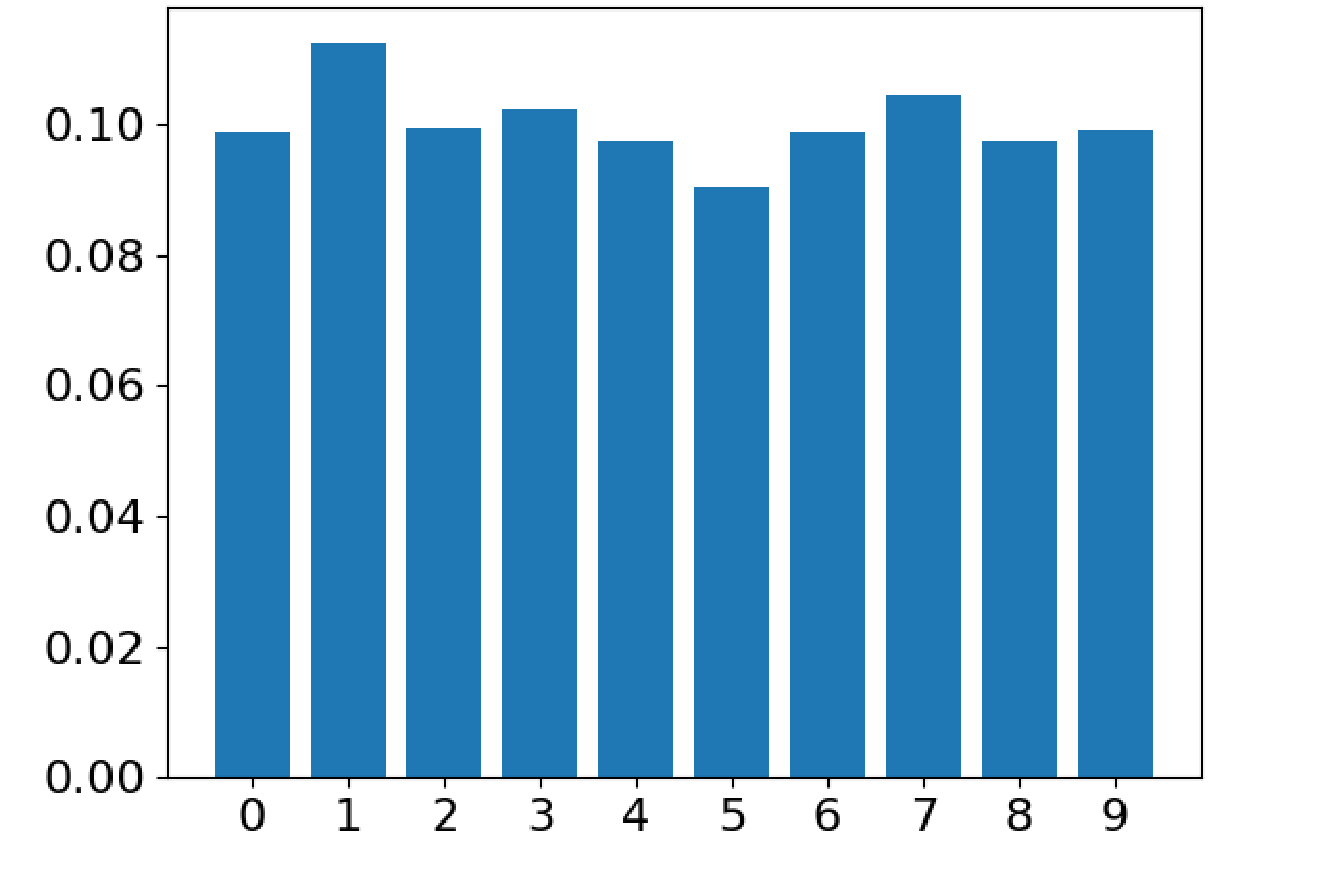
\includegraphics[width=\textwidth]{ChapterThree/mnist_dist}
		\caption{MNIST}
	\end{subfigure}
	\hfill
	\begin{subfigure}[b]{0.24\textwidth}  
		\centering 
		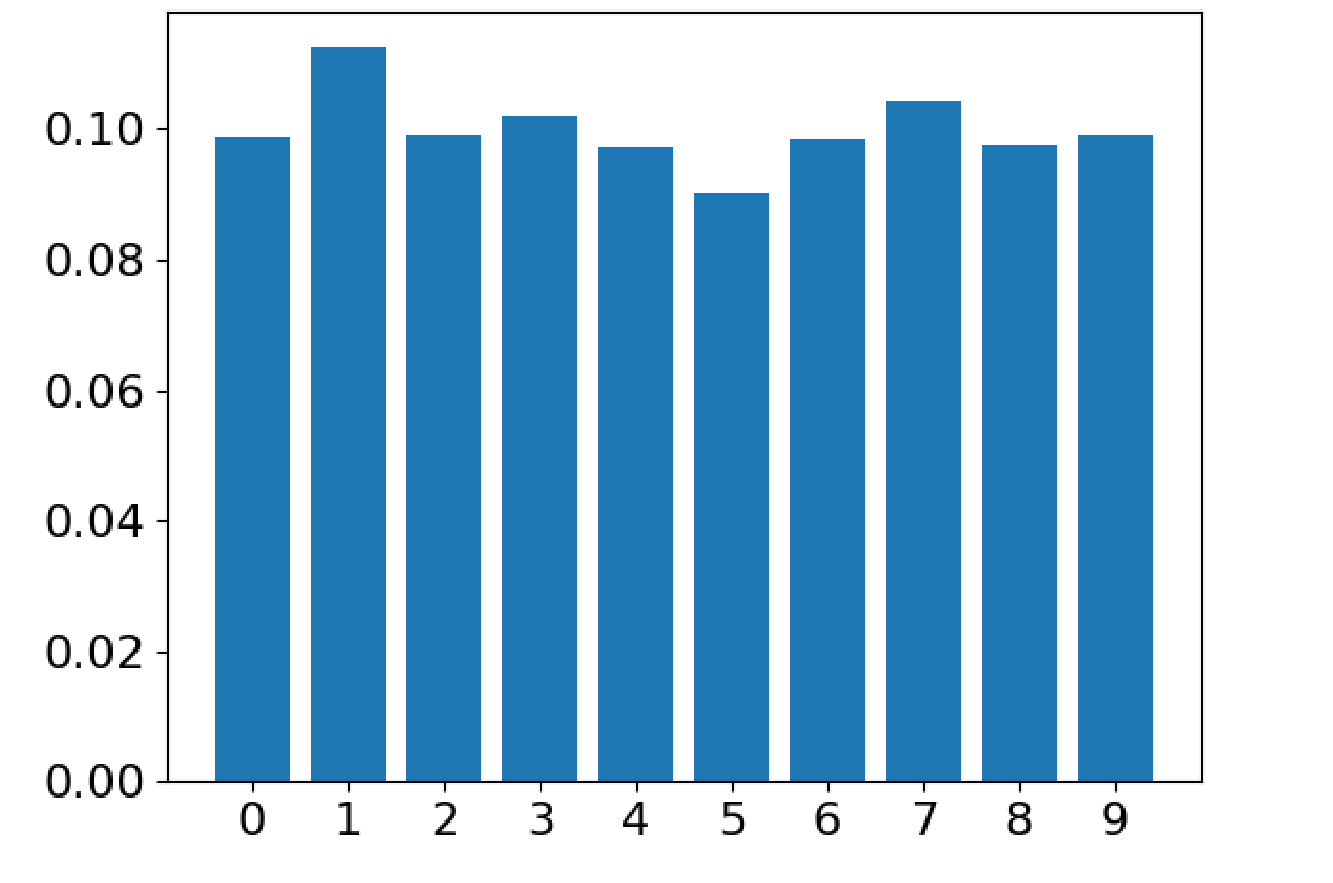
\includegraphics[width=\textwidth]{ChapterThree/mnist_m_dist}
		\caption{MNIST-M}
	\end{subfigure}
	\hfill
	\begin{subfigure}[b]{0.24\textwidth}   
		\centering 
		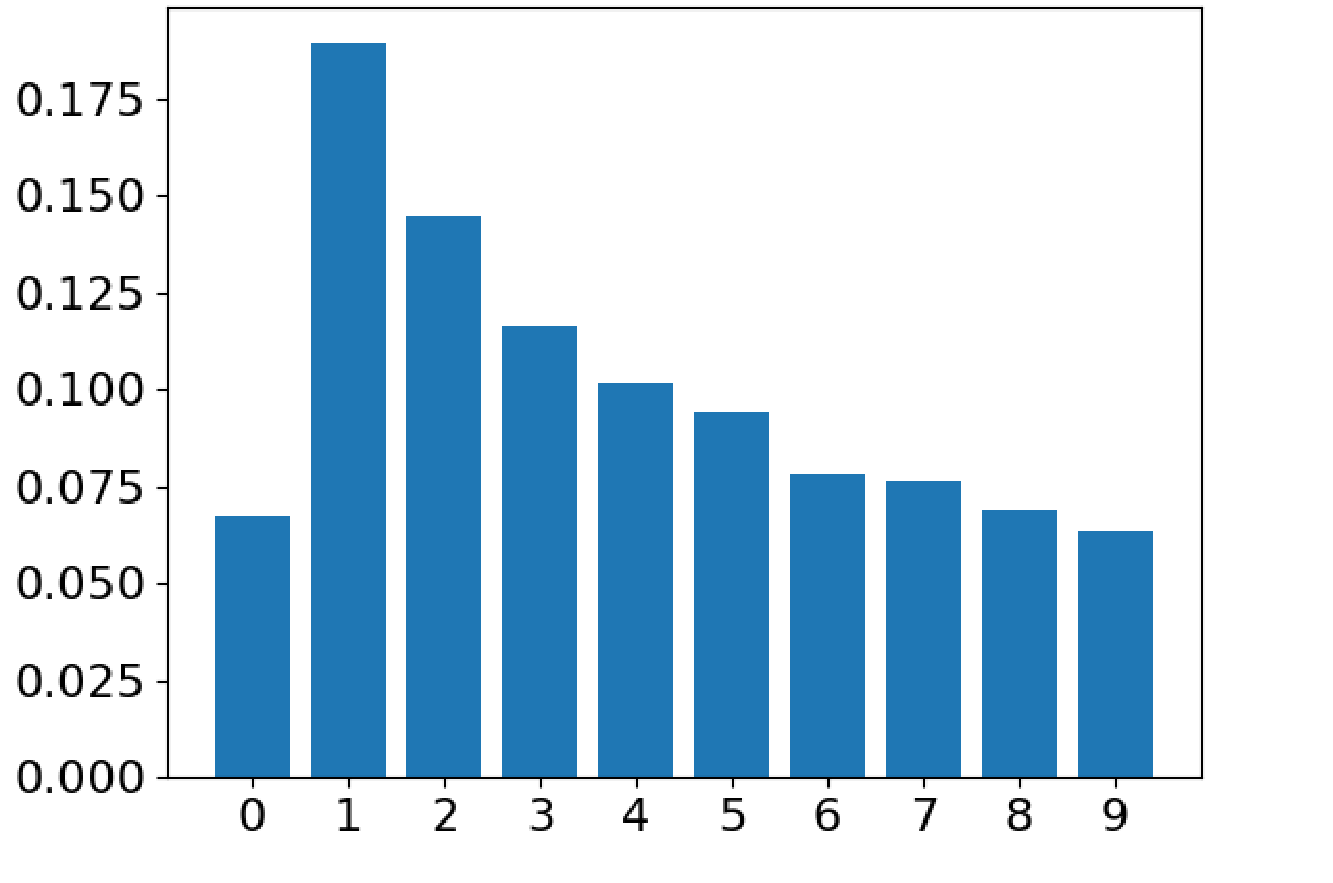
\includegraphics[width=\textwidth]{ChapterThree/svhn_dist}
		\caption{SVHN}
	\end{subfigure}
	\hfill
	\begin{subfigure}[b]{0.24\textwidth}   
		\centering 
		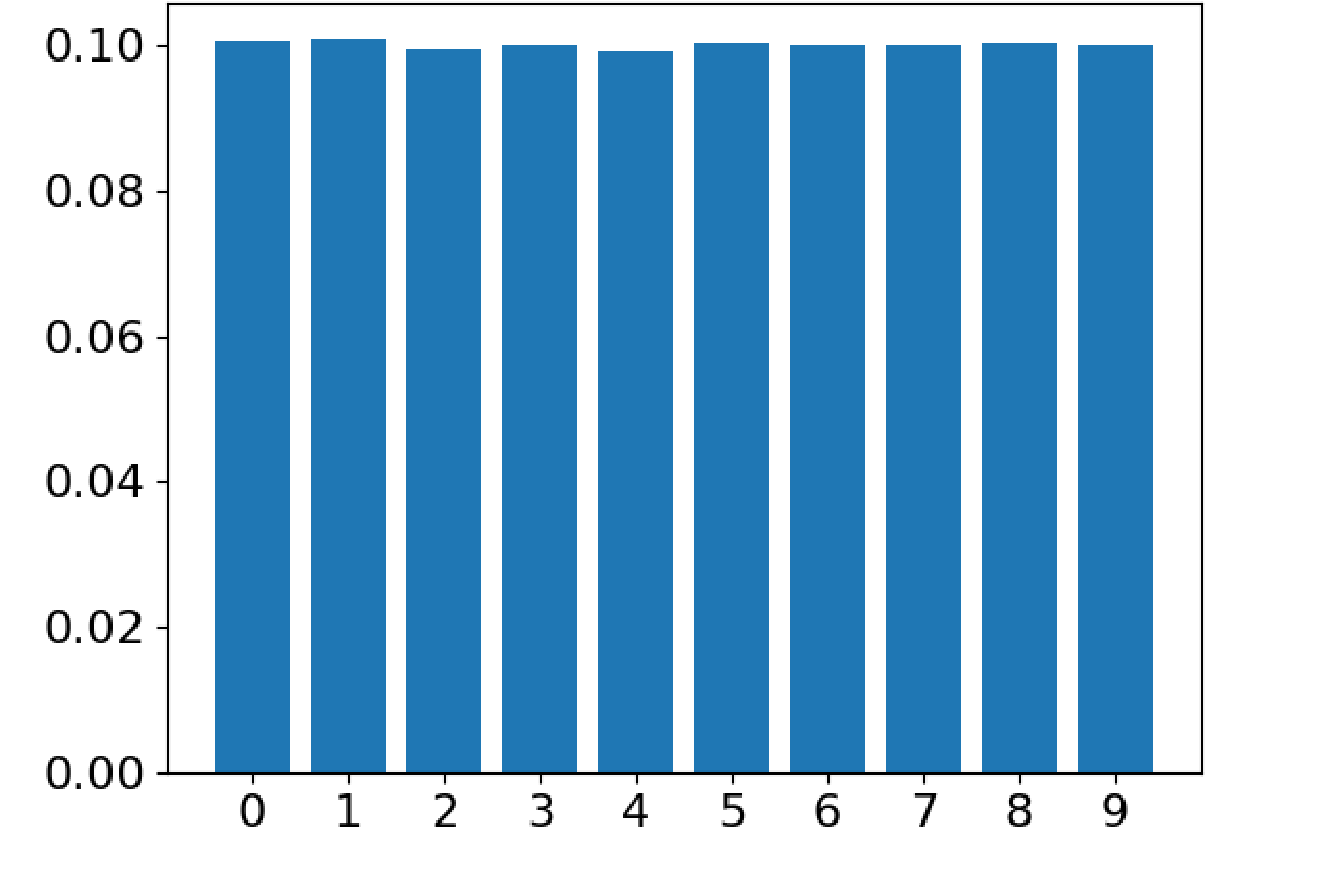
\includegraphics[width=\textwidth]{ChapterThree/synthdigits_dist}
		\caption{SynthDigits}
	\end{subfigure}
	\caption{Label distributions in the digits datasets.} 
	\label{fig:digits_dist}
\end{figure}

\begin{table}
	\centering
	\caption{Jensen-Shannon distances between the label distributions of each pair of digits domains. On each column, the largest distance is in bold and the smallest is underlined.}
	\small
	\begin{tabular}{l|cccc}
		& MNIST                & MNIST-M              & SVHN & SynthDigits \\ \hline
		MNIST       & $0$                  & $\underline{2.73 \cdot 10^{-4}}$ & $\underline{1.17 \cdot 10^{-1}}$     & $\underline{1.83 \cdot 10^{-2}}$            \\
		MNIST-M     & $\underline{2.73 \cdot 10^{-4}}$ & $0$                  & $\underline{1.17 \cdot 10^{-1}}$     & $1.84 \cdot 10^{-2}$            \\
		SVHN        & $\boldsymbol{1.17 \cdot 10^{-1}}$ & $\boldsymbol{1.17 \cdot 10^{-1}}$ & $0$                      & $\boldsymbol{1.26 \cdot 10^{-1}}$            \\
		SynthDigits & $1.83 \cdot 10^{-2}$ & $1.84 \cdot 10^{-2}$ & $\boldsymbol{1.26 \cdot 10^{-1}}$     & $0$ \\ \hline
		Average & $4.51 \cdot 10^{-2}$ &  $4.52 \cdot 10^{-2}$ & $1.20 \cdot 10^{-1}$ & $5.42 \cdot 10^{-2}$
	\end{tabular}
	\label{tab:digits_js}
\end{table}

\begin{figure}
	\centering
	\begin{subfigure}[b]{0.35\textwidth}
		\centering
		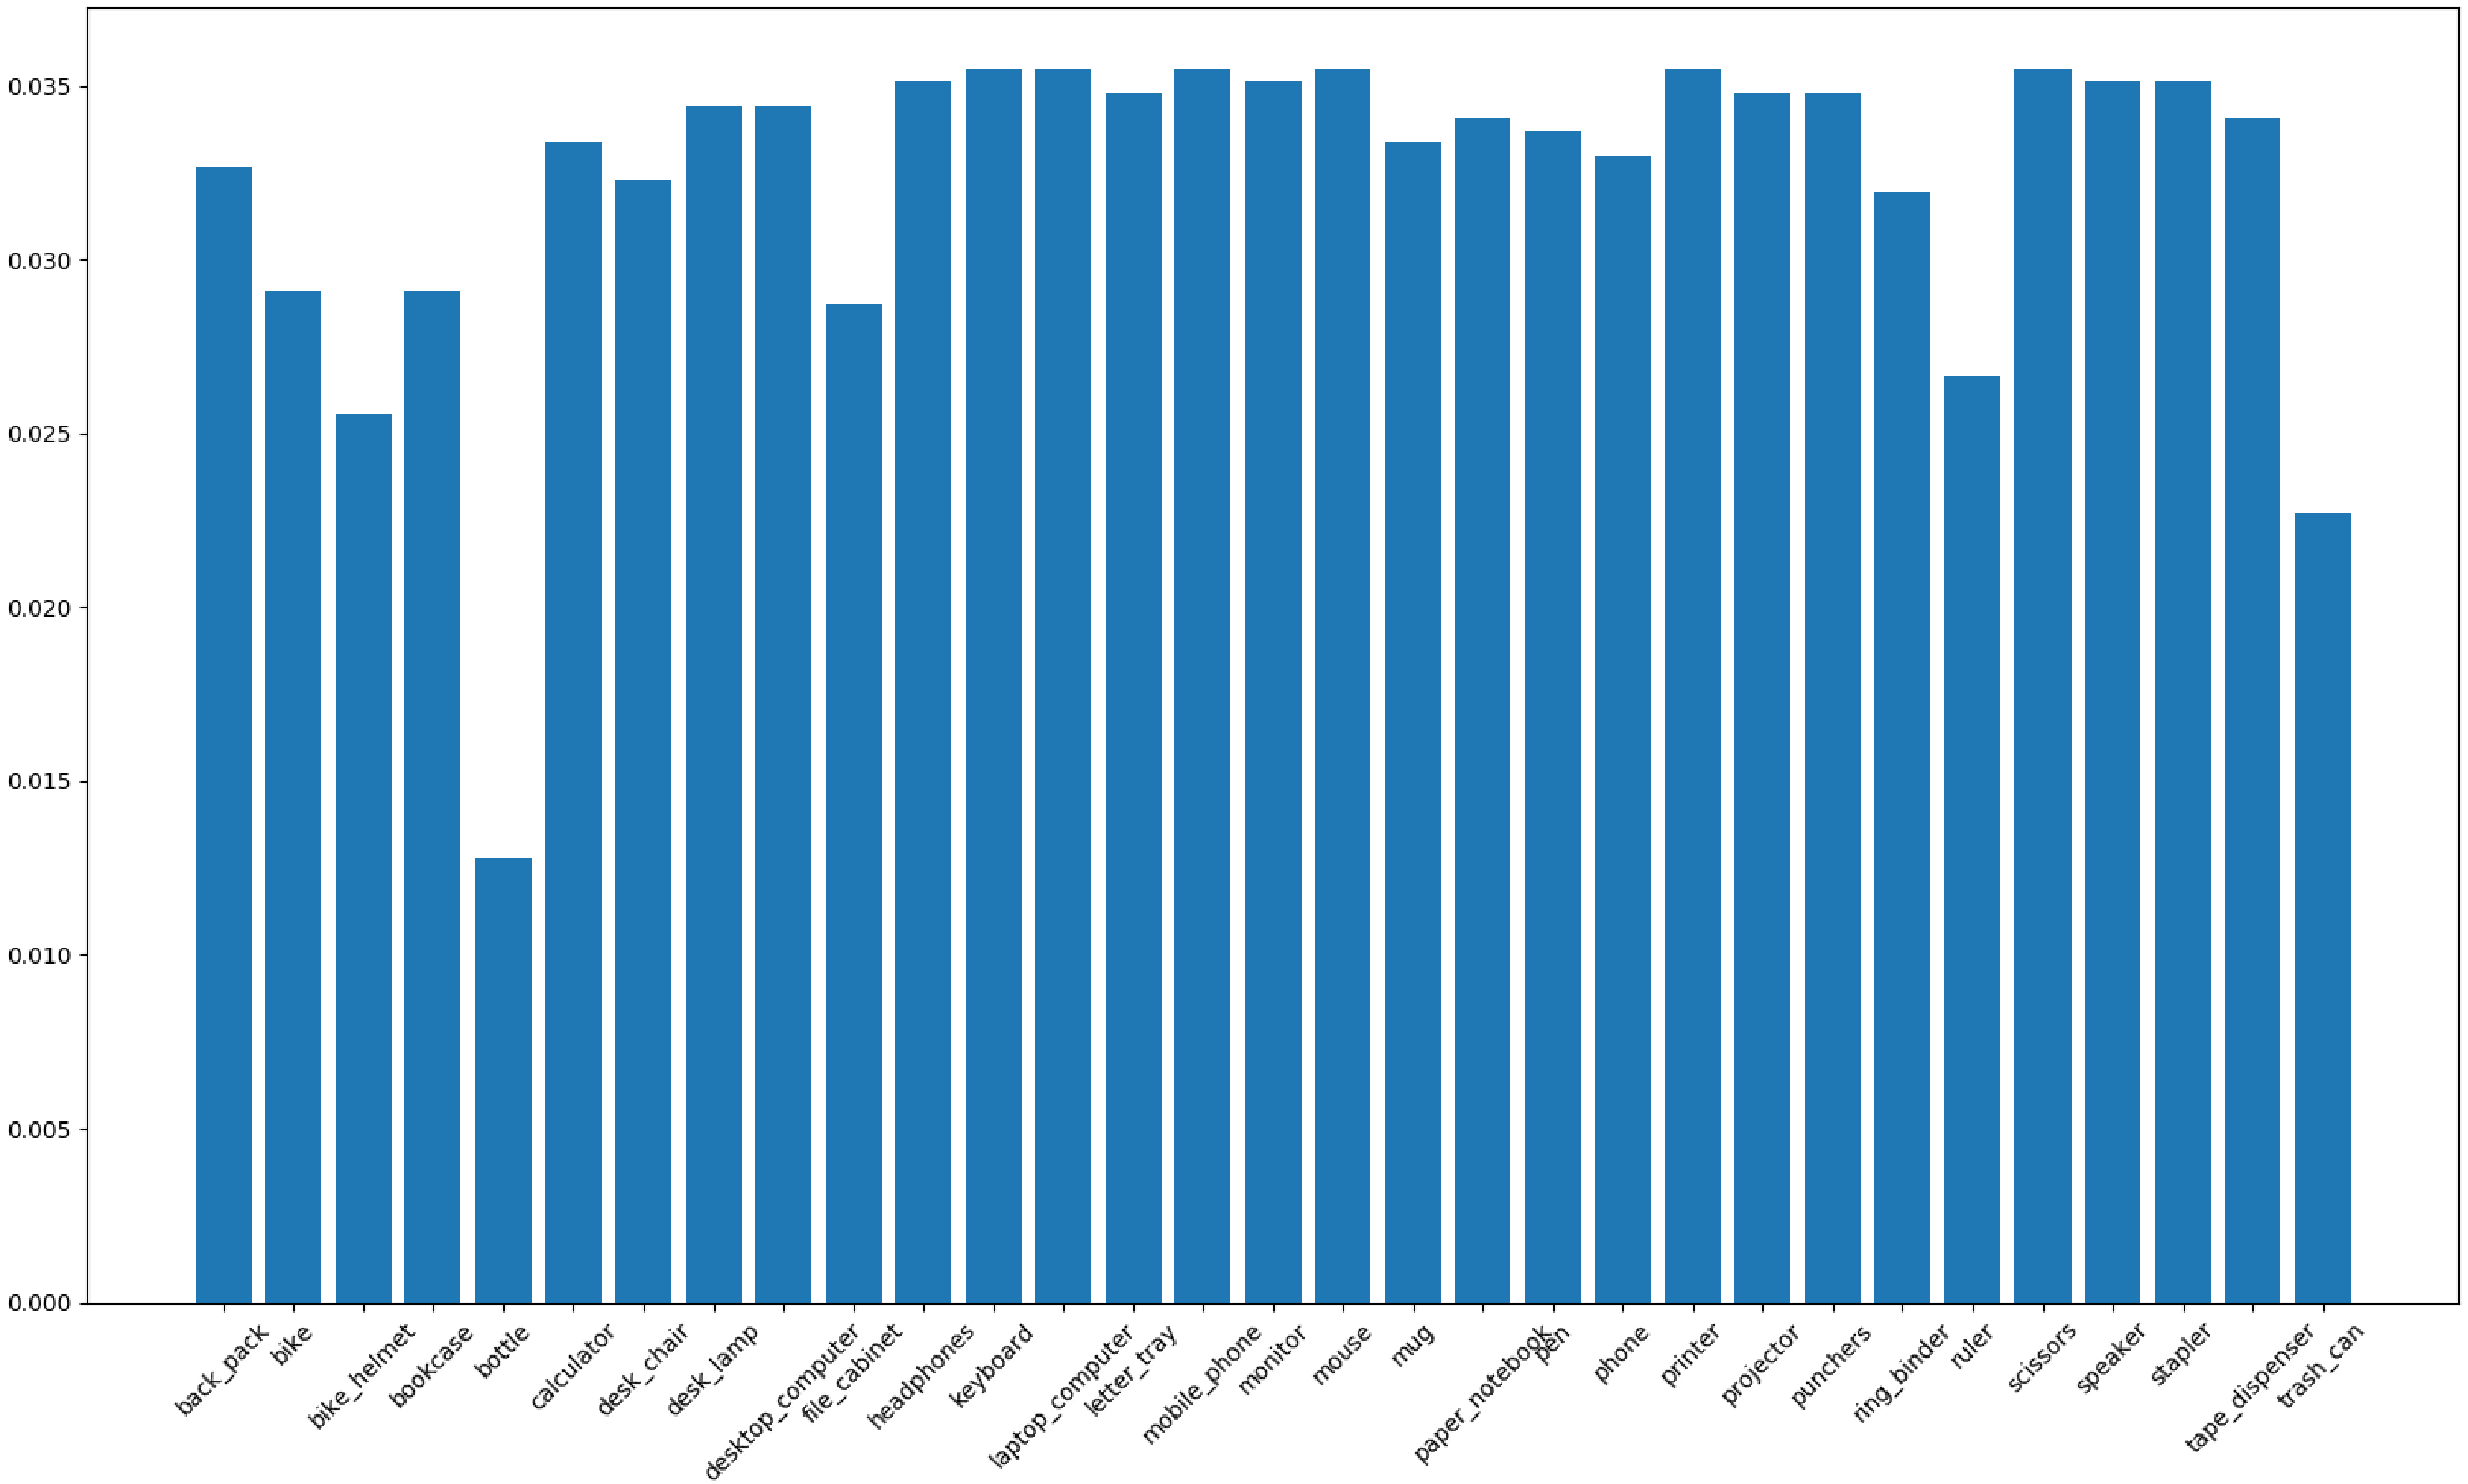
\includegraphics[width=\textwidth]{ChapterThree/amazon_dist}
		\caption{Amazon}
	\end{subfigure}
	\;%\hspace{-0.5cm}
	\begin{subfigure}[b]{0.35\textwidth}  
		\centering 
		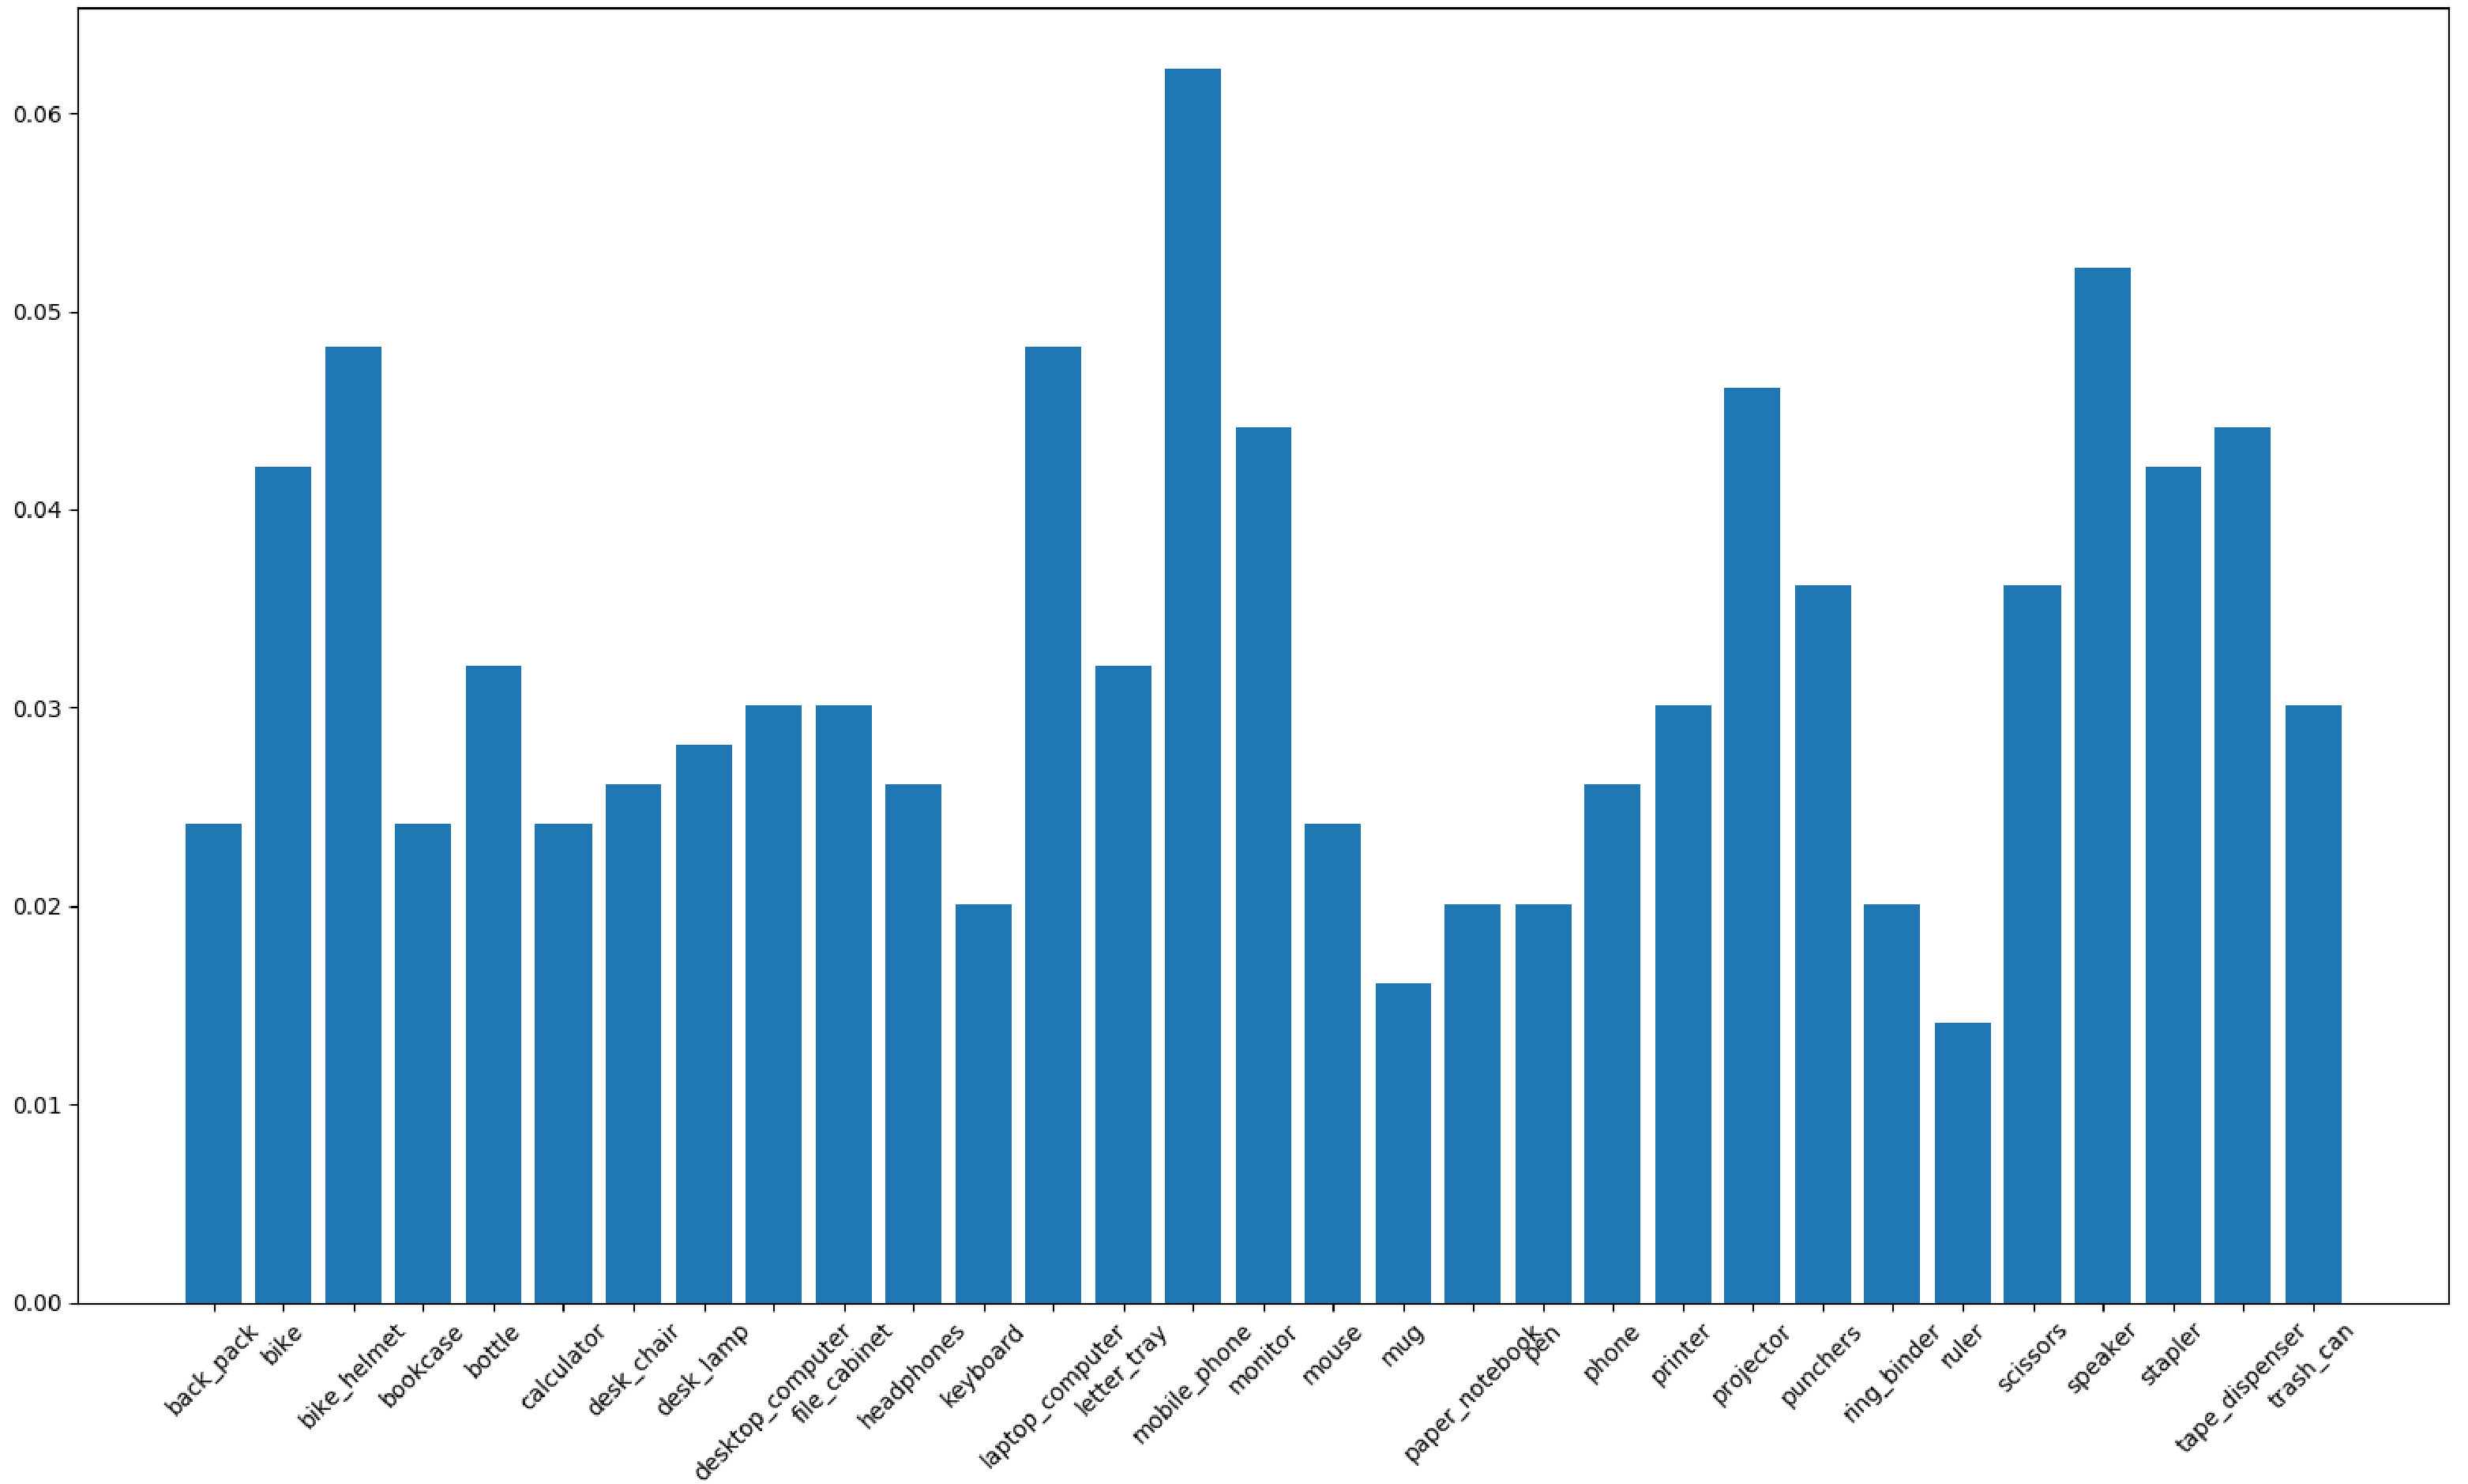
\includegraphics[width=\textwidth]{ChapterThree/dslr_dist}
		\caption{DSLR}
	\end{subfigure}
	\vskip\baselineskip
	\begin{subfigure}[b]{0.35\textwidth}   
		\centering 
		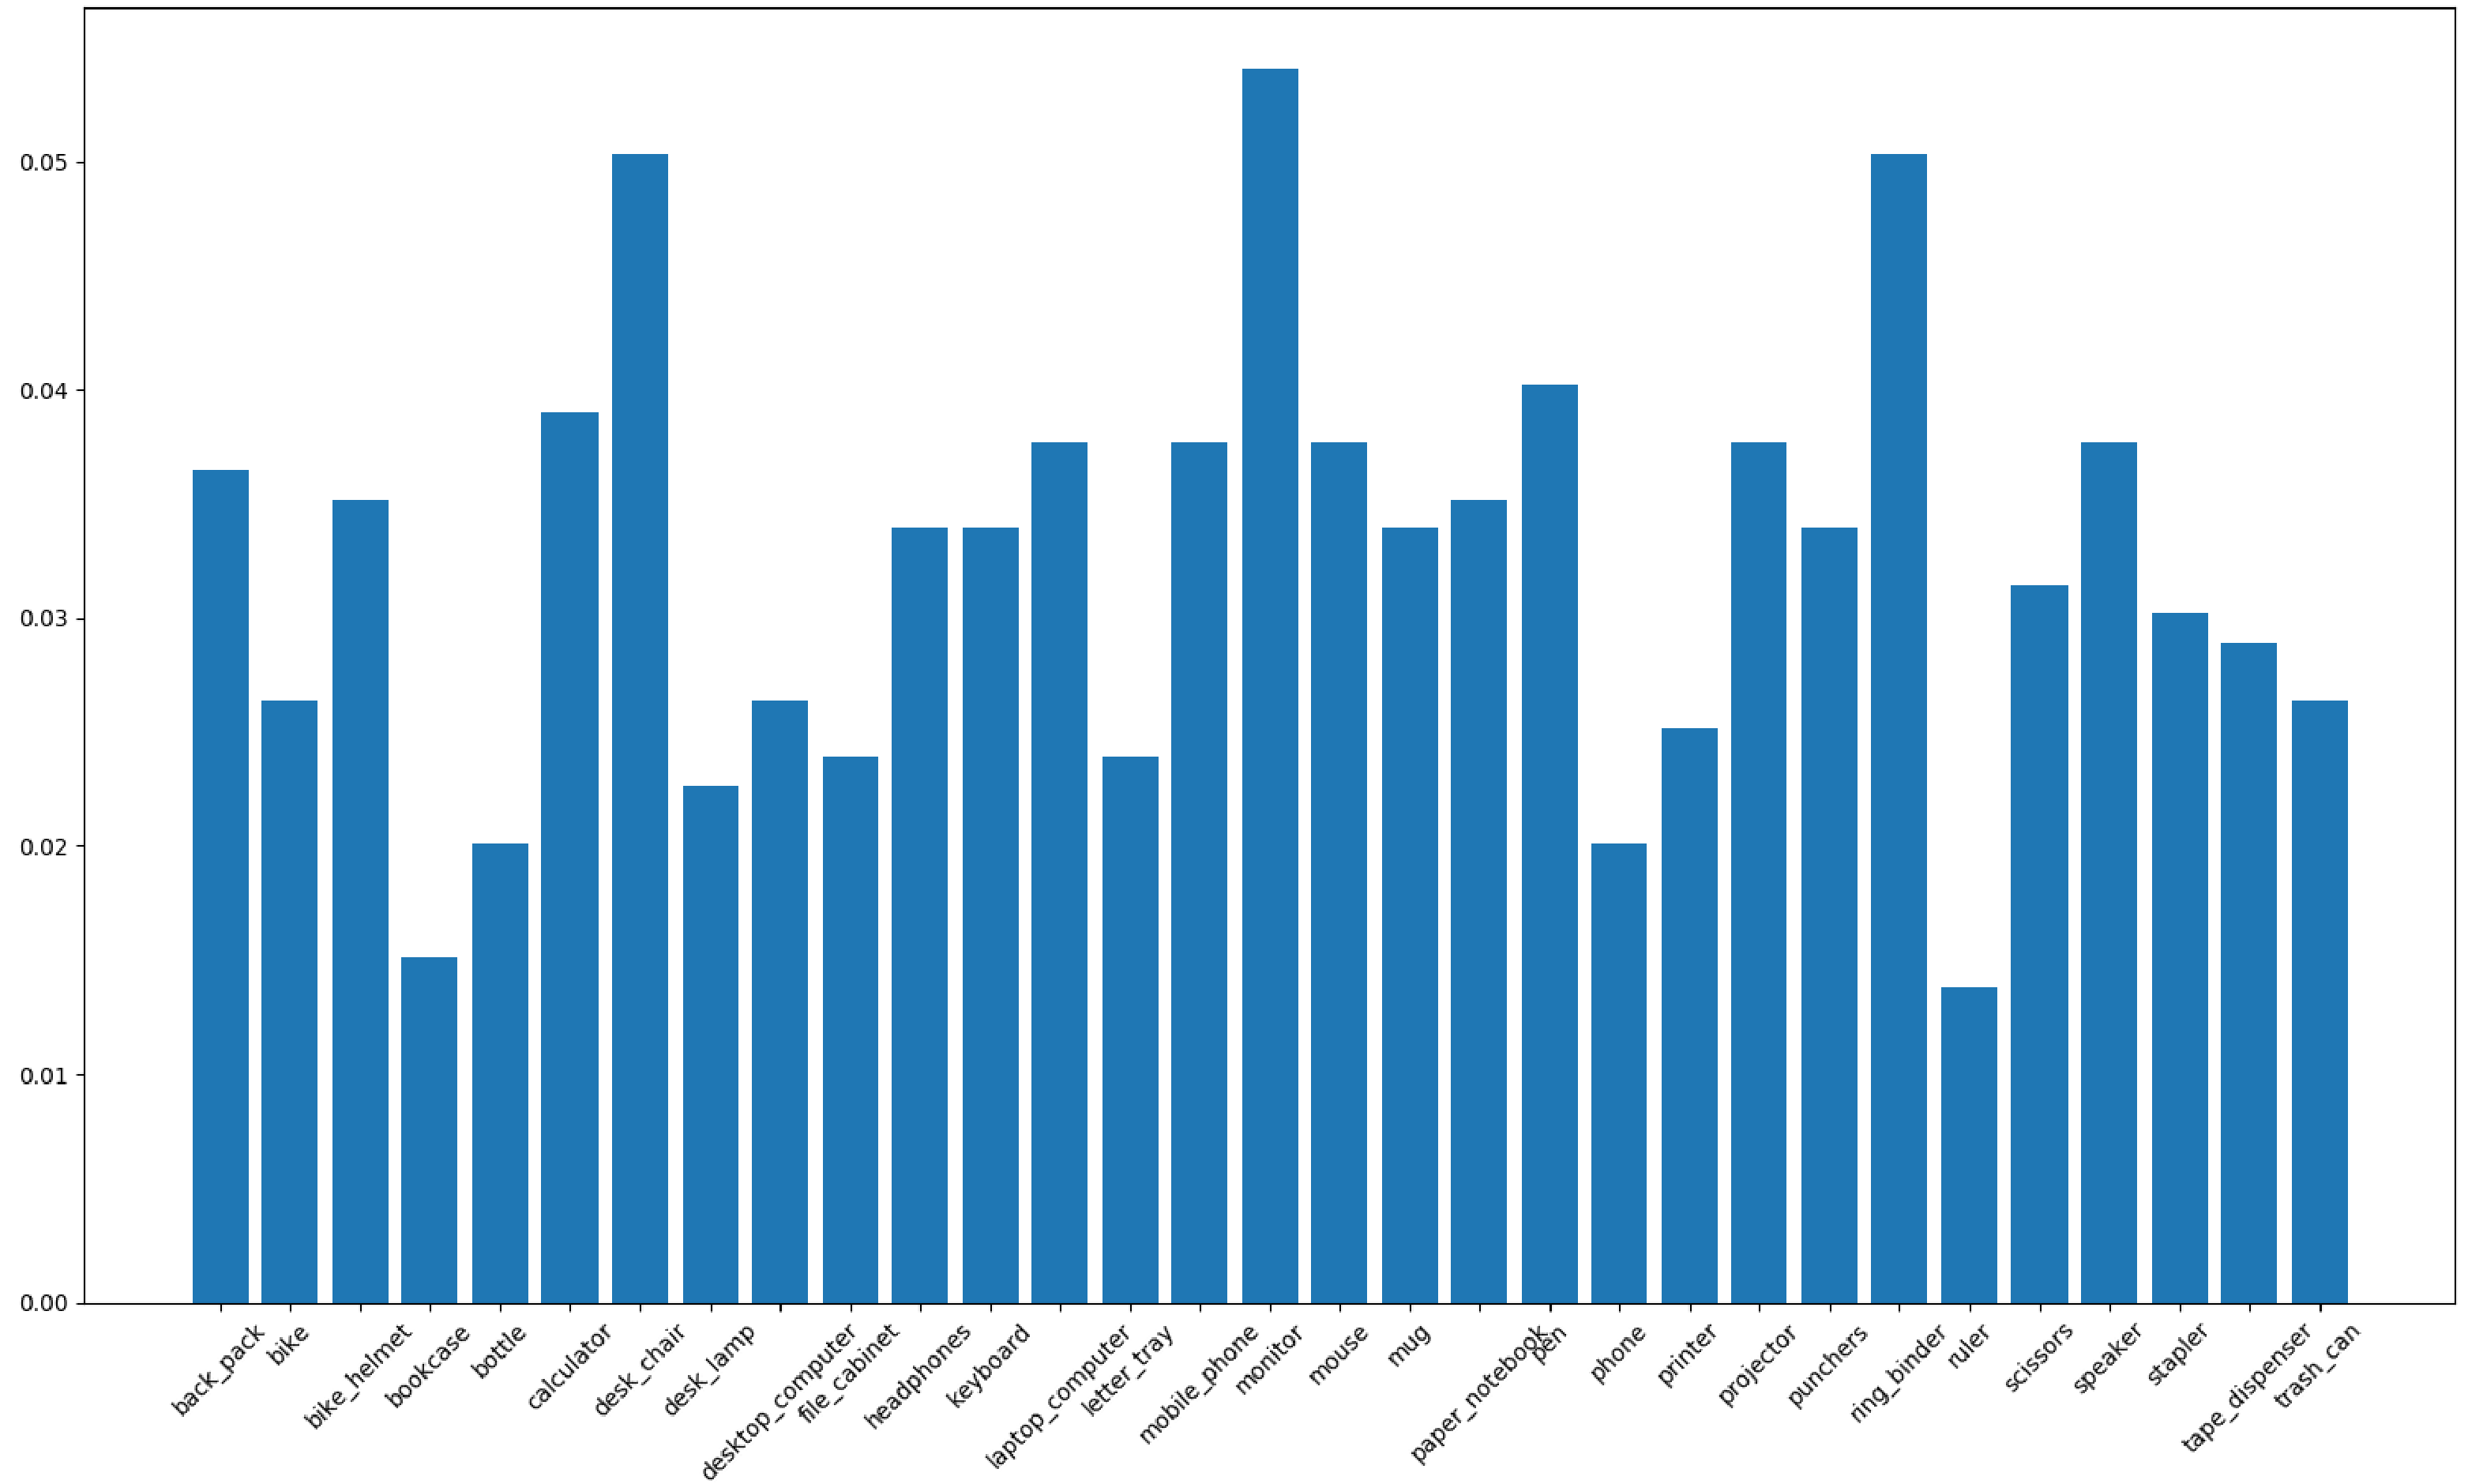
\includegraphics[width=\textwidth]{ChapterThree/webcam_dist}
		\caption{Webcam}
	\end{subfigure}
	\caption{Label distributions in Office-31.} 
	\label{fig:office_dist}
\end{figure}

\begin{table}
	\centering
	\caption{Jensen-Shannon distances between the label distributions of each pair of domains in Office-31. On each column, the largest distance is in bold.}
	\small
	\begin{tabular}{l|ccc}
		& Amazon                    & DSLR                      & Webcam                    \\ \hline
		Amazon & 0                         & $1.33 \cdot 10^{-1}$      & $9.76 \cdot 10^{-2}$      \\
		DSLR   & $\boldsymbol{1.33 \cdot 10^{-1}}$ & 0                         & $\boldsymbol{1.45 \cdot 10^{-1}}$ \\
		Webcam & $9.76 \cdot 10^{-2}$      & $\boldsymbol{1.45 \cdot 10^{-1}}$ & 0 \\ \hline
		Average & $1.15 \cdot 10^{-1}$ & $1.39 \cdot 10^{-1}$ & $1.21 \cdot 10^{-1}$
	\end{tabular}
	\label{tab:office_js}
\end{table}

\begin{figure}
	\centering
	\begin{subfigure}[b]{0.24\textwidth}
		\centering
		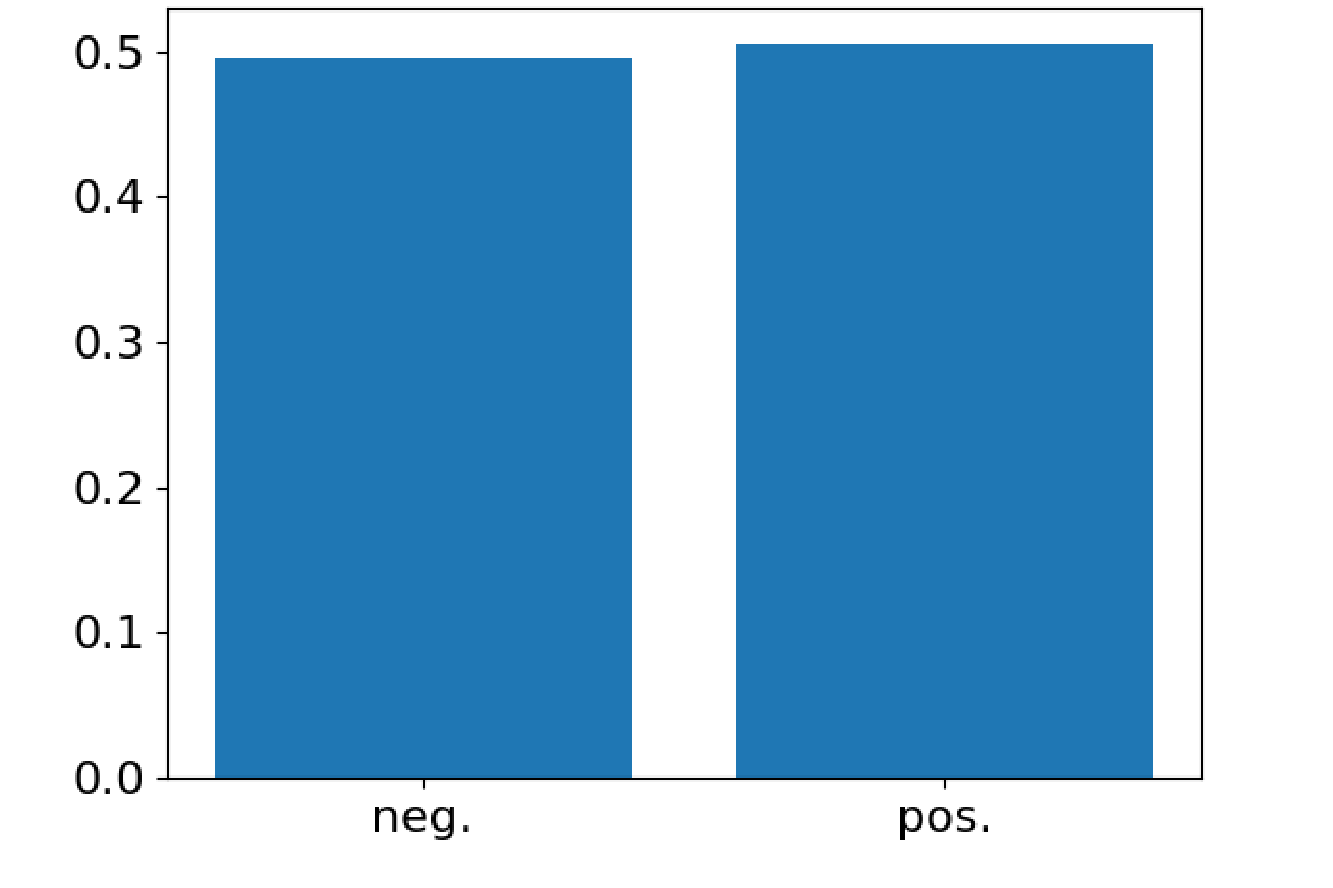
\includegraphics[width=\textwidth]{ChapterThree/books_dist}
		\caption{Books}
	\end{subfigure}
	\hfill
	\begin{subfigure}[b]{0.24\textwidth}  
		\centering 
		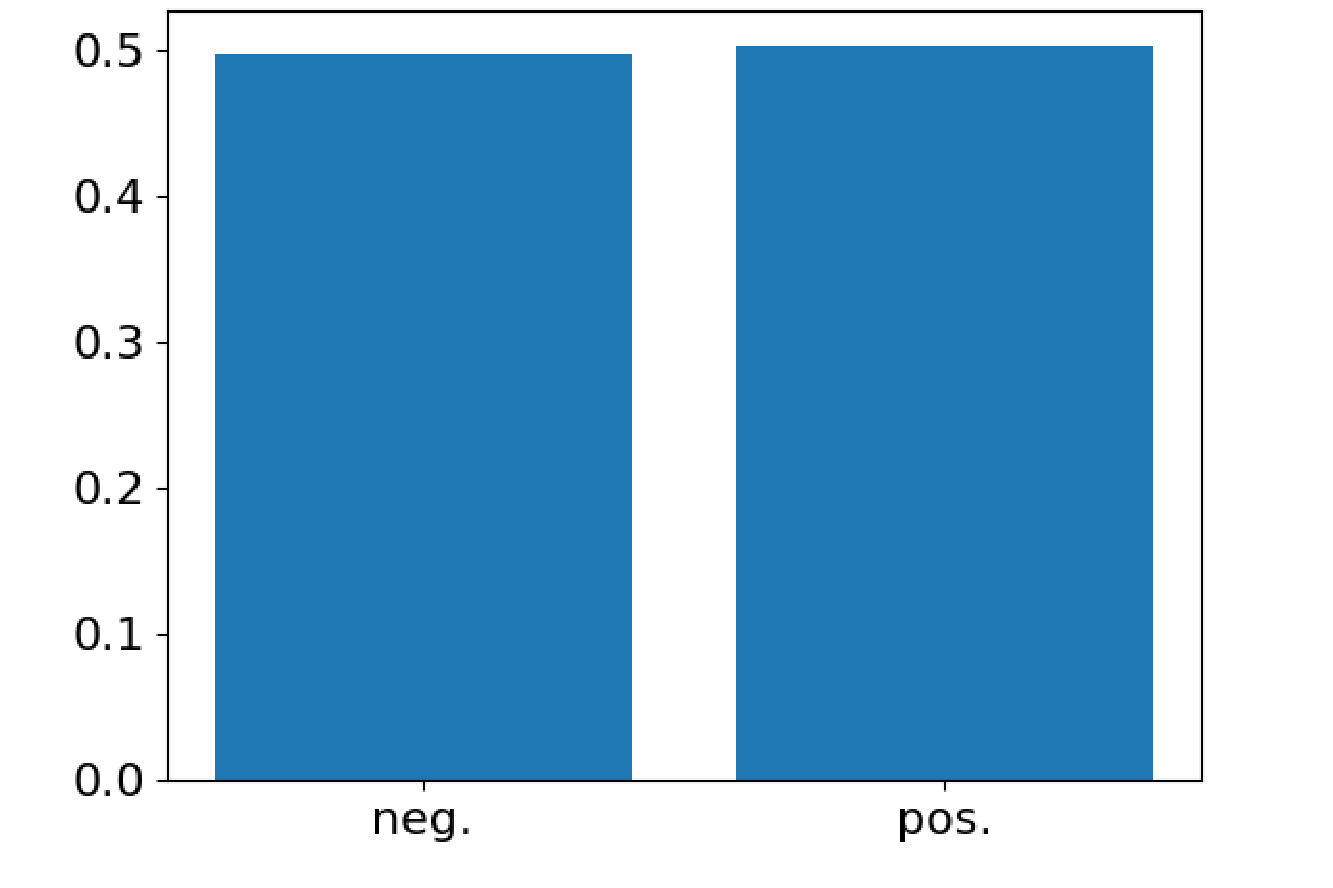
\includegraphics[width=\textwidth]{ChapterThree/dvd_dist}
		\caption{DVD}
	\end{subfigure}
	\hfill
	\begin{subfigure}[b]{0.24\textwidth}   
		\centering 
		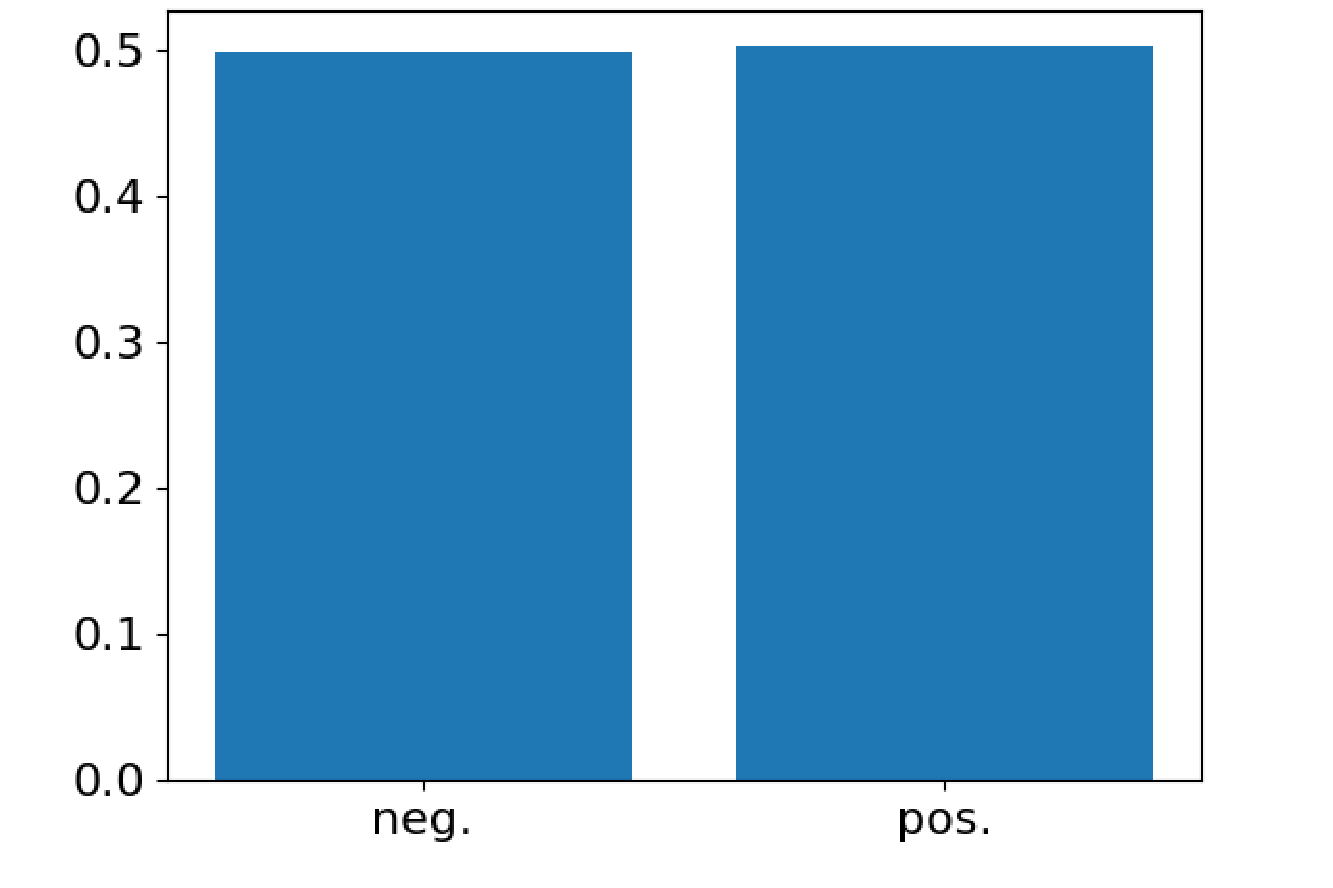
\includegraphics[width=\textwidth]{ChapterThree/electronics_dist}
		\caption{Electronics}
	\end{subfigure}
	\hfill
	\begin{subfigure}[b]{0.24\textwidth}   
		\centering 
		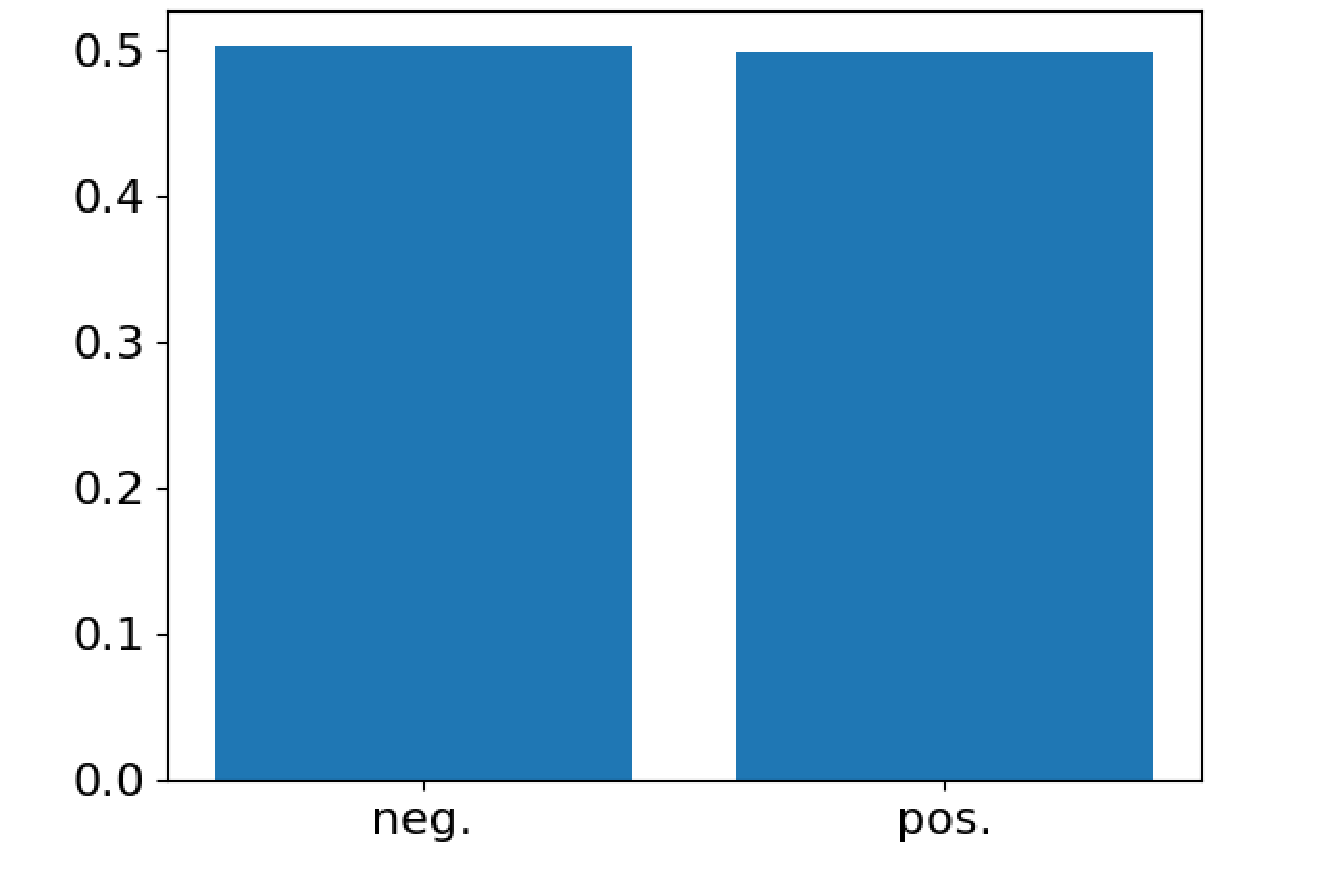
\includegraphics[width=\textwidth]{ChapterThree/kitchen_dist}
		\caption{Kitchen}
	\end{subfigure}
	\caption{Label distributions in Amazon Reviews.} 
	\label{fig:amazon_dist}
\end{figure}

\begin{table}
	\centering
	\caption{Jensen-Shannon distances between the label distributions of each pair of domains in Amazon Reviews. On each column, the largest distance is in bold and the smallest is underlined.}
	\small
	\begin{tabular}{l|cccc}
		& Books                & DVD                  & Electronics          & Kitchen              \\ \hline
		Books       & 0                    & $1.67 \cdot 10^{-3}$ & $1.93 \cdot 10^{-3}$ & $\boldsymbol{5.09 \cdot 10^{-3}}$ \\
		DVD         & $\underline{1.67 \cdot 10^{-3}}$ & 0                    & $\underline{2.53 \cdot 10^{-4}}$ & $3.42 \cdot 10^{-3}$ \\
		Electronics & $1.93 \cdot 10^{-3}$ & $\underline{2.53 \cdot 10^{-4}}$ & 0                    & $\underline{3.17 \cdot 10^{-3}}$ \\
		Kitchen     & $\boldsymbol{5.09 \cdot 10^{-3}}$ & $\boldsymbol{3.42 \cdot 10^{-3}}$ & $\boldsymbol{3.17 \cdot 10^{-3}}$ & 0 \\ \hline
		Average & $2.90 \cdot 10^{-3}$ & $1.78 \cdot 10^{-3}$ & $1.78 \cdot 10^{-3}$ & $3.89 \cdot 10^{-3}$
	\end{tabular}
	\label{tab:amazon_js}
\end{table}

\begin{table}
	\centering
	\caption{Jensen-Shannon distances between the label distributions of each pair of domains in the DomainNet dataset. On each column, the largest distance is in bold and the smallest is underlined.}
	\small
	\hspace*{-0.50in}
	\begin{tabular}{l|cccccc}
		& \textit{clp}                & \textit{inf}              & \textit{pnt} & \textit{qdr} & \textit{rel} & \textit{skt} \\ \hline
		\textit{clp} & $0$ & $3.14 \cdot 10^{-1}$ & $3.34 \cdot 10^{-1}$     & $1.98 \cdot 10^{-1}$ & $2.31 \cdot 10^{-1}$ & $2.60 \cdot 10^{-1}$         \\
		\textit{inf} & $3.14 \cdot 10^{-1}$ & $0$ & $\boldsymbol{3.79 \cdot 10^{-1}}$ & $\boldsymbol{2.83 \cdot 10^{-1}}$ & $\boldsymbol{3.03 \cdot 10^{-1}}$ & $\boldsymbol{3.26 \cdot 10^{-1}}$ \\
		\textit{pnt} & $\boldsymbol{3.34 \cdot 10^{-1}}$ & $\boldsymbol{3.79 \cdot 10^{-1}}$ & $0$ & $2.77 \cdot 10^{-1}$ & $2.99 \cdot 10^{-1}$ & $3.10 \cdot 10^{-1}$ \\
		\textit{qdr} & $\underline{1.98 \cdot 10^{-1}}$ & $\underline{2.83 \cdot 10^{-1}}$ & $\underline{2.77 \cdot 10^{-1}}$ & $0$ & $\underline{1.35 \cdot 10^{-1}}$ & $\underline{2.27 \cdot 10^{-1}}$ \\
		\textit{rel}  & $2.31 \cdot 10^{-1}$ & $3.03 \cdot 10^{-1}$ & $2.99 \cdot 10^{-1}$ & $\underline{1.35 \cdot 10^{-1}}$ & $0$ & $2.67 \cdot 10^{-1}$ \\
		\textit{skt}  & $2.60 \cdot 10^{-1}$ & $3.26 \cdot 10^{-1}$ & $3.10 \cdot 10^{-1}$ & $2.27 \cdot 10^{-1}$ & $2.67 \cdot 10^{-1}$ & $0$ \\ \hline
		Average & $2.67 \cdot 10^{-1}$ & $3.21 \cdot 10^{-1}$ & $3.20 \cdot 10^{-1}$ & $2.24 \cdot 10^{-1}$ & $2.47 \cdot 10^{-1}$ & $2.78 \cdot 10^{-1}$ \\
	\end{tabular}
	\label{tab:domainnet_js}
\end{table}

\subsection{Effect of over-training}
\label{sec:overtrain}
When the label distributions differ across domains, training the feature extractor and domain discriminator for a large number of iterations tends to lead to an increased target error. This is a direct effect of the curse of domain-invariant representations and it has been verified experimentally in \cite{Zhao2019}.

In this experiment, we want to evaluate if the increased robustness of the feature extractor provided by the adopted consistency regularization helps to mitigate this issue. For this purpose, we use Office-31 since it is fairly small and therefore easy to overtrain and the label distributions across domains are significantly skewed (see \ref{sec:label_dist}). We train our model and two baselines (MDAN~\citep{Zhao2018} and MODA) for 60 epochs and we observe the evolution of the model accuracy on the target data. The plots are shown in \Figref{fig:overtrain}. As we see there, in MODA-FM the accuracy keeps stable after reaching the maximum in all domains. Contrarily, in MODA and especially in MDAN, the accuracy tends to decay after reaching the maximum. These observations strongly suggest that MODA-FM succeeds on mitigating the curse of domain-invariant representations. In MODA the problem is less pronounced than in MDAN probably because the latter will continue optimizing itself until it can produce domain-invariant representations for all source domains, whereas the former will simply ignore the hardest source domains by assigning them a low weight (possibly even zero).

\begin{figure}
	\centering
	\hspace*{-0.30in}
	\begin{subfigure}[b]{0.32\textwidth}
		\begin{tikzpicture}[scale=0.58, every node/.style={scale=0.58}]
		\begin{axis}[
		enlargelimits=false,
		legend style={at={(0.45,0.1)},anchor=south west,font=\large},
		xlabel=\huge epoch, xmin=0, xmax=60, xtick={0,10,20,30,40,50,60},
		ylabel=\huge accuracy, ymin=0.55, ymax=0.75, ytick={0.55,0.6,0.65,0.7,0.75},
		grid=both, grid style={line width=.1pt, draw=gray!10},
		]   
		\addplot[color=myblue,smooth,thick]table[x=Epoch, y=MDAN, col sep=comma]{Figures/ChapterThree/amazon_long.txt};
		\addlegendentry{MDAN ($\pgfmathprintnumber{\slopeMDAN}$)}
		
		\addplot[color=myorange,smooth,thick]table[x=Epoch, y=MixMDAN, col sep=comma]{Figures/ChapterThree/amazon_long.txt};
		\addlegendentry{MODA ($\pgfmathprintnumber{\slopeMODA}$)}
		
		\addplot[color=mygreen,smooth,thick]table[x=Epoch, y=Ours, col sep=comma]{Figures/ChapterThree/amazon_long.txt};
		\addlegendentry{MODA-FM ($\pgfmathprintnumber{\slopeMODAFM}$)}
		
		\addplot[color=gray,dashed] table [col sep = comma,y={create col/linear regression={y=1}},skip first n=2]{Figures/ChapterThree/amazon_long.txt};
		\xdef\slopeMDAN{\pgfplotstableregressiona}
		\addplot[color=gray,dashed] table [col sep = comma,y={create col/linear regression={y=2}},skip first n=2]{Figures/ChapterThree/amazon_long.txt};
		\xdef\slopeMODA{\pgfplotstableregressiona}
		\addplot[color=gray,dashed] table [col sep = comma,y={create col/linear regression={y=3}},skip first n=2]{Figures/ChapterThree/amazon_long.txt};
		\xdef\slopeMODAFM{\pgfplotstableregressiona}
		\end{axis}
		\end{tikzpicture}
		\caption{Amazon}
	\end{subfigure}
	\hfill%
	\begin{subfigure}[b]{0.32\textwidth}
		\centering
		\hspace*{-0.30in}
		\begin{tikzpicture}[scale=0.58, every node/.style={scale=0.58}]
		\begin{axis}[
		enlargelimits=false,
		legend style={at={(0.45,0.1)},anchor=south west,font=\large},
		xlabel=\huge epoch, xmin=0, xmax=60, xtick={0,10,20,30,40,50,60},
		ylabel=\huge accuracy, ymin=0.8, ymax=1, ytick={0.8,0.85,0.9,0.95,1},
		grid=both, grid style={line width=.1pt, draw=gray!10},
		]   
		\addplot[color=myblue,smooth,thick]table[x=Epoch, y=MDAN, col sep=comma]{Figures/ChapterThree/dslr_long.txt};
		\addlegendentry{MDAN ($\pgfmathprintnumber{\slopeMDAN}$)}
		
		\addplot[color=myorange,smooth,thick]table[x=Epoch, y=MixMDAN, col sep=comma]{Figures/ChapterThree/dslr_long.txt};
		\addlegendentry{MODA ($\pgfmathprintnumber{\slopeMODA}$)}
		
		\addplot[color=mygreen,smooth,thick]table[x=Epoch, y=Ours, col sep=comma]{Figures/ChapterThree/dslr_long.txt};
		\addlegendentry{MODA-FM ($\pgfmathprintnumber{\slopeMODAFM}$)}
		
		\addplot[color=gray,dashed] table [col sep = comma,y={create col/linear regression={y=1}},skip first n=2]{Figures/ChapterThree/dslr_long.txt};
		\xdef\slopeMDAN{\pgfplotstableregressiona}
		\addplot[color=gray,dashed] table [col sep = comma,y={create col/linear regression={y=2}},skip first n=2]{Figures/ChapterThree/dslr_long.txt};
		\xdef\slopeMODA{\pgfplotstableregressiona}
		\addplot[color=gray,dashed] table [col sep = comma,y={create col/linear regression={y=3}},skip first n=2]{Figures/ChapterThree/dslr_long.txt};
		\xdef\slopeMODAFM{\pgfplotstableregressiona}
		\end{axis}
		\end{tikzpicture}
		\caption{DSLR}
	\end{subfigure}
	\hfill%
	\begin{subfigure}[b]{0.32\textwidth}
		\centering
		\hspace*{-0.30in}
		\begin{tikzpicture}[scale=0.58, every node/.style={scale=0.58}]
		\begin{axis}[
		enlargelimits=false,
		legend style={at={(0.45,0.1)},anchor=south west,font=\large},
		xlabel=\huge epoch, xmin=0, xmax=60, xtick={0,10,20,30,40,50,60},
		ylabel=\huge accuracy, ymin=0.8, ymax=1, ytick={0.8,0.85,0.9,0.95,1},
		grid=both, grid style={line width=.1pt, draw=gray!10},
		]   
		\addplot[color=myblue,smooth,thick]table[x=Epoch, y=MDAN, col sep=comma]{Figures/ChapterThree/webcam_long.txt};
		\addlegendentry{MDAN ($\pgfmathprintnumber{\slopeMDAN}$)}
		
		\addplot[color=myorange,smooth,thick]table[x=Epoch, y=MixMDAN, col sep=comma]{Figures/ChapterThree/webcam_long.txt};
		\addlegendentry{MODA ($\pgfmathprintnumber{\slopeMODA}$)}
		
		\addplot[color=mygreen,smooth,thick]table[x=Epoch, y=Ours, col sep=comma]{Figures/ChapterThree/webcam_long.txt};
		\addlegendentry{MODA-FM ($\pgfmathprintnumber{\slopeMODAFM}$)}
		
		\addplot[color=gray,dashed] table [col sep = comma,y={create col/linear regression={y=1}},skip first n=2]{Figures/ChapterThree/webcam_long.txt};
		\xdef\slopeMDAN{\pgfplotstableregressiona}
		\addplot[color=gray,dashed] table [col sep = comma,y={create col/linear regression={y=2}},skip first n=2]{Figures/ChapterThree/webcam_long.txt};
		\xdef\slopeMODA{\pgfplotstableregressiona}
		\addplot[color=gray,dashed] table [col sep = comma,y={create col/linear regression={y=3}},skip first n=2]{Figures/ChapterThree/webcam_long.txt};
		\xdef\slopeMODAFM{\pgfplotstableregressiona}
		\end{axis}
		\end{tikzpicture}
		\caption{Webcam}
	\end{subfigure}
	\caption{Test accuracy over 60 training epochs for our model and two baselines in Office-31. The tendency line for each curve is also shown (dashed lines) and the respective slope is indicated in brackets in each plot legend. The domain indicated below each plot is the target.}
	\label{fig:overtrain}
\end{figure}

\subsection{Hyperparameter sensitivity analysis}
\label{sec:hyperparam}
Our model comprises three main hyperparameters: $\mu_d$, $\mu_s$ and $\mu_c$. The hyperparameter $\mu_d$ controls the relative weight of the domain discriminator loss and is present in every work on adversarial DA, thus its effect has already been studied extensively. For this reason, we focus on the effect of $\mu_s$ and $\mu_c$. We use the digits datasets and evaluate the accuracy on each target domain while varying either $\mu_s$ or $\mu_c$ and keeping the other one constant at the optimal value.

A sufficiently large value of $\mu_s$ forces $\valpha$ to converge to a vector with all components equal to $1/M$, weighting all source domains equally. Setting $\mu_s$ close to zero corresponds to the most optimistic scenario: the sparsity penalization is dropped and so, after sufficiently many training iterations, $\valpha$ would converge to a one-hot vector, choosing the source domain with the minimum difference of classification and discrimination losses ($\gL_{class} - \mu_d\gL_{disc}$). \Figref{fig:hyperparam_mu_s} shows that, for MNIST, similar results are obtained with any of those strategies. The fact that digits classification in MNIST is significantly easier than in any of the remaining datasets likely explains this behavior. Domain adaptation for MNIST-M is slightly favored by smaller values of $\mu_s$, meaning that a more optimistic approach works better here. For SVHN, the opposite holds and the results are very poor when low sparsity regularization is employed. There is even a strong discontinuity in the accuracy plot for this domain around $\mu_s \approx 0.2$. This discontinuity divides situations where $\valpha$ collapses into the easiest source domain ($\mu_s < 0.2$) and those where it does not collapse ($\mu_s > 0.2$). We elaborate more on this in \ref{sec:alpha_evol}. In all cases, we observe that a $\mu_s \in [0.2, 0.6]$ provides near-optimal results.

The effect of varying $\mu_c$ is plotted in \Figref{fig:hyperparam_mu_c}. Values of $\mu_c$ close to zero drop the consistency regularization and, therefore, we obtain results close to those of MODA. Significant performance gains are obtained for $\mu_c > 0.01$ and the optimal is reached for $\mu_c \in [0.4, 1.0]$ for all domains.

\begin{figure}
	\centering
	\hspace*{-0.30in}
	\begin{subfigure}[b]{0.45\textwidth}
		\centering
		\begin{tikzpicture}[scale=0.8, every node/.style={scale=0.58}]
		\begin{semilogxaxis}[xmin=5e-5, xmax=50, ymin=0, ymax=1.05, domain=1e-5:20, ylabel=\large accuracy,
		scaled x ticks=real:1e-3,
		xtick scale label code/.code={},
		log x ticks with fixed point/.style={
			xticklabel={
				\pgfkeys{/pgf/fpu=true}
				\pgfmathparse{exp(\tick)}%
				\pgfmathprintnumber[fixed relative, precision=3]{\pgfmathresult}
				\pgfkeys{/pgf/fpu=false}
			}
		},
		legend style={at={(0.65,0.1)},anchor=south west,font=\normalsize},
		grid=both, grid style={line width=.1pt, draw=gray!10}]
		
		\addplot[color=myblue,only marks,sharp plot,mark=*]table[x index={0}, y index={1}, col sep=comma, skip first n=2]{Figures/ChapterThree/mu_s.txt};
		\addlegendentry{MNIST}
		
		\addplot[color=myorange,only marks,sharp plot,mark=*]table[x index={0}, y index={2}, col sep=comma, skip first n=2]{Figures/ChapterThree/mu_s.txt};
		\addlegendentry{MNIST-M}
		
		\addplot[color=mygreen,only marks,sharp plot,mark=*]table[x index={0}, y index={3}, col sep=comma, skip first n=2]{Figures/ChapterThree/mu_s.txt};
		\addlegendentry{SVHN}
		\end{semilogxaxis}
		\end{tikzpicture}
		\caption{$\mu_s$}
		\label{fig:hyperparam_mu_s}
	\end{subfigure}
	\hfill%
	\begin{subfigure}[b]{0.45\textwidth}
		\centering
		\begin{tikzpicture}[scale=0.8, every node/.style={scale=0.58}]
		\begin{semilogxaxis}[xmin=5e-5, xmax=50, ymin=0, ymax=1.05, domain=1e-5:20, ylabel=\large accuracy,
		scaled x ticks=real:1e-3,
		xtick scale label code/.code={},
		log x ticks with fixed point/.style={
			xticklabel={
				\pgfkeys{/pgf/fpu=true}
				\pgfmathparse{exp(\tick)}%
				\pgfmathprintnumber[fixed relative, precision=3]{\pgfmathresult}
				\pgfkeys{/pgf/fpu=false}
			}
		},
		legend style={at={(0.65,0.1)},anchor=south west,font=\normalsize},
		grid=both, grid style={line width=.1pt, draw=gray!10}]
		
		\addplot[color=myblue,only marks,sharp plot,mark=*]table[x index={0}, y index={1}, col sep=comma, skip first n=2]{Figures/ChapterThree/mu_c.txt};
		\addlegendentry{MNIST}
		
		\addplot[color=myorange,only marks,sharp plot,mark=*]table[x index={0}, y index={2}, col sep=comma, skip first n=2]{Figures/ChapterThree/mu_c.txt};
		\addlegendentry{MNIST-M}
		
		\addplot[color=mygreen,only marks,sharp plot,mark=*]table[x index={0}, y index={3}, col sep=comma, skip first n=2]{Figures/ChapterThree/mu_c.txt};
		\addlegendentry{SVHN}
		\end{semilogxaxis}
		\end{tikzpicture}
		\caption{$\mu_c$}
		\label{fig:hyperparam_mu_c}
	\end{subfigure}
	\caption{Test accuracy as a function of hyperparameters $\mu_s$ (a) and $\mu_c$ (b) using the digits datasets. The domain corresponding to each line is the target.}
	\label{fig:hyperparam}
\end{figure}

\subsection{Evolution of the source weights}
\label{sec:alpha_evol}
Here, we study the evolution of the source weights $\valpha$ over training. The behavior is determined by the evolution of the classification and discrimination losses of each source domain and also by the choice of the hyperparameter $\mu_s$. The effect of varying $\mu_s$ on the model performance was analyzed in \ref{sec:hyperparam}. Now, we are interested in observing the dynamics of $\valpha$ over the training epochs, for different source domains, using the corresponding optimal $\mu_s$. We use the digits datasets for this purpose and we present the results in \Figref{fig:alpha_train}.

For MNIST, where the lowest $\mu_s$ is used, we observe that the mixture coefficients rapidly collapse into the easiest source domain (SynthDigits). Nonetheless, in \ref{sec:hyperparam} we have observed that the target accuracy for MNIST was almost insensitive to the choice of $\mu_s$, meaning that using only the data from the easiest source domain or weighting all source domains equally would produce identical results. When we take MNIST-M and SVHN as target domains, with a slightly increased $\mu_s$, a different behavior occurs. Early in the training process, the weight for the easiest source domain (MNIST) increases rapidly, following the fast decrease in the corresponding loss. Later, as the loss for the easiest source domain plateaus and the remaining keep decreasing, the  weights for the remaining active source domains start to increase. This behavior explains the discontinuity we have observed in the plot of target accuracy vs. $\mu_s$ for SVHN (\Figref{fig:hyperparam_mu_s}): if $\mu_s$ is sufficiently small to allow $\valpha$ to rapidly collapse into MNIST, the data of the remaining source domains is simply discarded for the remaining of the training process and the corresponding weights will never increase.

\begin{figure}
	\centering
	%\hspace*{-0.50in}
	\begin{subfigure}[b]{0.32\textwidth}
		\begin{tikzpicture}[scale=0.58, every node/.style={scale=0.58}]
		\begin{axis}[
		enlargelimits=false,
		legend style={at={(0.65,0.1)},anchor=south west,font=\large},
		xlabel=\huge epoch, xmin=0, xmax=60, xtick={0,10,20,30,40,50,60},
		ylabel=\huge $\valpha$, ymin=0., ymax=1., 
		grid=both, grid style={line width=.1pt, draw=gray!10},
		title=\text{\huge $\mu_s=0.1$}
		]   
		\addplot[color=myorange,smooth,thick]table[x=Epoch, y=MNIST_M, col sep=comma]{Figures/ChapterThree/mnist_coef.txt};
		\addlegendentry{MNIST-M}
		
		\addplot[color=mygreen,smooth,thick]table[x=Epoch, y=SVHN, col sep=comma]{Figures/ChapterThree/mnist_coef.txt};
		\addlegendentry{SVHN}
		
		\addplot[color=myred,smooth,thick]table[x=Epoch, y=SynthDigits, col sep=comma]{Figures/ChapterThree/mnist_coef.txt};
		\addlegendentry{SynthDigits}
		\end{axis}
		\end{tikzpicture}
		\caption{MNIST}
	\end{subfigure}
	\hfill%
	\begin{subfigure}[b]{0.32\textwidth}
		\centering
		\begin{tikzpicture}[scale=0.58, every node/.style={scale=0.58}]
		\begin{axis}[
		enlargelimits=false,
		legend style={at={(0.65,0.1)},anchor=south west,font=\large},
		xlabel=\huge epoch, xmin=0, xmax=60, xtick={0,10,20,30,40,50,60},
		ylabel=\huge $\valpha$, ymin=0., ymax=1.,
		grid=both, grid style={line width=.1pt, draw=gray!10},
		title=\text{\huge$\mu_s=0.2$}
		]   
		\addplot[color=myblue,smooth,thick]table[x=Epoch, y=MNIST, col sep=comma]{Figures/ChapterThree/mnist_m_coef.txt};
		\addlegendentry{MNIST}
		
		\addplot[color=mygreen,smooth,thick]table[x=Epoch, y=SVHN, col sep=comma]{Figures/ChapterThree/mnist_m_coef.txt};
		\addlegendentry{SVHN}
		
		\addplot[color=myred,smooth,thick]table[x=Epoch, y=SynthDigits, col sep=comma]{Figures/ChapterThree/mnist_m_coef.txt};
		\addlegendentry{SynthDigits}
		\end{axis}
		\end{tikzpicture}
		\caption{MNIST-M}
	\end{subfigure}
	\hfill%
	\begin{subfigure}[b]{0.32\textwidth}
		\centering
		\begin{tikzpicture}[scale=0.58, every node/.style={scale=0.58}]
		\begin{axis}[
		enlargelimits=false,
		legend style={at={(0.65,0.1)},anchor=south west,font=\large},
		xlabel=\huge epoch, xmin=0, xmax=60, xtick={0,10,20,30,40,50,60},
		ylabel=\huge $\valpha$, ymin=0., ymax=1,
		grid=both, grid style={line width=.1pt, draw=gray!10},
		title=\text{\huge$\mu_s=0.9$}
		]   
		\addplot[color=myblue,smooth,thick]table[x=Epoch, y=MNIST, col sep=comma]{Figures/ChapterThree/svhn_coef.txt};
		\addlegendentry{MNIST}
		
		\addplot[color=myorange,smooth,thick]table[x=Epoch, y=MNIST_M, col sep=comma]{Figures/ChapterThree/svhn_coef.txt};
		\addlegendentry{MNIST-M}
		
		\addplot[color=myred,smooth,thick]table[x=Epoch, y=SynthDigits, col sep=comma]{Figures/ChapterThree/svhn_coef.txt};
		\addlegendentry{SynthDigits}
		\end{axis}
		\end{tikzpicture}
		\caption{SVHN}
	\end{subfigure}
	\caption{Source weights $\valpha$ for each domain over 60 training epochs in the digits datasets. The target domain and the value of $\mu_s$ that was used are indicated below and above each plot, respectively.}
	\label{fig:alpha_train}
\end{figure}

\subsection{Network architectures}
\label{sec:arch}
The following notation is used to designate network layers: \texttt{Conv(n, k)} -- 2-D convolutional layer with \texttt{n} output channels, square kernels with size \texttt{k}, and unit stride, followed by a rectified linear activation; \texttt{MaxPool(k)} -- 2-D max-pooling over non-overlapping regions of $\texttt{k} \times \texttt{k}$ pixels; \texttt{AdaptAvgPool(k)} -- 2-D adaptive average pooling where the output size is $\texttt{k} \times \texttt{k}$ pixels. \texttt{FC(n)} -- fully-connected layer with $\texttt{n}$ output neurons, followed by a rectified linear activation except for output layers; \texttt{Dropout(p)} -- dropout layer where $\texttt{p}$ is the probability of zeroing an element. A gradient reversal layer is present at the input of the domain discriminator in all models. All classifiers and domain discriminators are followed by a softmax layer that maps the output to the corresponding class probabilities.

\paragraph{Digits classification} Input images have shape $3 \times 32 \times 32$. Feature extractor: \texttt{Conv(64, 3)}~$\rightarrow$ \texttt{MaxPool(2)}~$\rightarrow$ \texttt{Conv(128, 3)}~$\rightarrow$ \texttt{MaxPool(2)}~$\rightarrow$ \texttt{Conv(256, 3)}. Task classifier: \texttt{MaxPool(2)}~$\rightarrow$ \texttt{Conv(256, 3)}~$\rightarrow$ \texttt{FC(2048)}~$\rightarrow$ \texttt{FC(1024)}~$\rightarrow$ \texttt{FC(10)}. Domain discriminator: \texttt{MaxPool(2)}~$\rightarrow$ \texttt{FC(2048)}~$\rightarrow$ \texttt{FC(2048)}~$\rightarrow$ \texttt{FC(1024)}~$\rightarrow$ \texttt{FC(2)}.

\paragraph{Object classification (Office-31 dataset)} Input images have shape $3 \times 256 \times 256$. Feature extractor: ResNet-50 up to stage~3. Task classifier / domain discriminator: ResNet-50 stage~4~$\rightarrow$ \texttt{AdaptAvgPool(1)}~$\rightarrow$ \texttt{FC(\#classes)}, where $\texttt{\#classes} = 31$ for the task classifier and $\texttt{\#classes} = 2$ for the domain discriminator.

\paragraph{Sentiment analysis (Amazon Reviews dataset)} Input features have dimension $5000$. Feature extractor: \texttt{Dropout(p)}~$\rightarrow$ \texttt{FC(1000)}~$\rightarrow$ \texttt{Dropout(p)}~$\rightarrow$ \texttt{FC(500)}~$\rightarrow$ \texttt{Dropout(p)}~$\rightarrow$ \texttt{FC(100)}~$\rightarrow$ \texttt{Dropout(p)}, where $\texttt{p} = 0$ except for producing the augmented samples used in the consistency regularization. Task classifier / domain discriminator: \texttt{FC(2)}.

\paragraph{Large scale object classification (DomainNet dataset)} Input images have shape $3 \times 192 \times 192$. Feature extractor: ResNet-152 up to stage~3. Task classifier / domain discriminator: ResNet-152 stage~4~$\rightarrow$ \texttt{AdaptAvgPool(1)}~$\rightarrow$ \texttt{FC(\#classes)}, where $\texttt{\#classes} = 345$ for the task classifier and $\texttt{\#classes} = 2$ for the domain discriminator.

\subsection{Choice of hyperparameters}
\label{sec:cross_val}
\Tableref{tab:hyperparameters} presents the values assigned to each hyperparameter. For some hyperparameters in a given dataset, a set or range of values is presented instead of a single value, meaning that the value for that hyperparameter was selected via cross-validation on the given set/range. This cross-validation consisted on 20 iterations of random search for each experiment, where no data from the target domain was used and each source domain was taken as target in turn. The hyperparameter combination that yielded the best average result was chosen.

\begin{table}
	\centering
	\caption{Values and search ranges for all hyperparameters in all experiments.}
	\label{tab:hyperparameters}
	\small
	\hspace*{-0.30in}
	\begin{tabular}{r|cccc}
		\multicolumn{1}{l|}{Hyperparameter} & Digits                & Office-31             & Amazon Reviews & DomainNet         \\ \hline
		$\mu_d$~(8)                            & $[10^{-4}, 10^{0}]$   & $[10^{-4}, 10^{0}]$   & $[10^{-4}, 10^{0}]$  & $10^{-2}$  \\ \hdashline[0.5pt/5pt]
		$\mu_s$~(8)                             & $[10^{-5}, 10^{0}]$   & $10^{-2}$             & $[10^{-6}, 10^{-1}]$ & $10^{-1}$  \\ \hdashline[0.5pt/5pt]
		$\mu_c$~(16)                             & $[10^{-2}, 10^{0}]$   & $[10^{-2}, 10^{0}]$   & $[10^{-2}, 10^{0}]$ & $10^{-1}$   \\ \hdashline[0.5pt/5pt]
		$\tau$~(15)                              & $0.9$                 & $0.9$                 & $0.9$  & $0.9$                \\ \hdashline[0.5pt/5pt]
		optimizer                           & AdaDelta              & AdaDelta              & AdaDelta & AdaDelta             \\ \hdashline[0.5pt/5pt]
		no. epochs                          & $\{10, 20, \dots, 60\}$ & $\{10, 15, \dots, 60\}$ & $\{5, 10, \dots, 40\}$ & $100$\\ \hdashline[0.5pt/5pt]
		learning rate                         & $0.1$             & $0.1$             & $1.0$ & $0.01$              \\ \hdashline[0.5pt/5pt]
		batch size                          & $8$                   & $8$                   & $20$  & $8$                  \\ \hdashline[0.5pt/5pt]
		RandAugment: $n$                    & $2$                   & $2$                   & n.a. & $2$                   \\ \hdashline[0.5pt/5pt]
		RandAugment: $m_{\text{min}}$       & $3$                   & $3$                   & n.a. &  $3$                 \\ \hdashline[0.5pt/5pt]
		RandAugment: $m_{\text{max}}$       & $10$                  & $10$                  & n.a.  &  $10$                \\ \hdashline[0.5pt/5pt]
		dropout: $p_{\text{min}}$           & n.a.                  & n.a.                  & $0.2$  & n.a.                 \\ \hdashline[0.5pt/5pt]
		dropout: $p_{\text{max}}$           & n.a.                  & n.a.                  & $0.8$  & n.a.                
	\end{tabular}
\end{table}


\subsection{Image transformations}
\label{sec:img_transf}
The list of image transformations used in RandAugment is provided in~\Tableref{tab:randaugment}. The cutout transformation is the first transformation to be applied to every image. This transformation occludes a randomly located square region with a length equal to $30\%$ of the image length. The remaining $n$ transformations are chosen at random from the provided list. All transformations were normalized such that a transformation of magnitude $m = 0$ corresponds to the identity (i.e., unchanged image) and a magnitude $m = 30$ (maximum admissible value) corresponds to the maximum distortion. We implemented the image transformations using the Python Imaging Library (PIL).

\begin{savenotes}
	\begin{table}[!h]
		\centering
		\caption{RandAugment image transformations and respective ranges.}
		\label{tab:randaugment}
		\small
		\begin{tabular}{r|c||rc}
			\multicolumn{1}{c|}{Transformation} & Range         & \multicolumn{1}{c|}{Transformation} & \multicolumn{1}{c}{Range} \\ \hline
			AutoContrast                        & $\{0, 1\}$    & \multicolumn{1}{r|}{Rotate}      & $[-30^{\circ}, 30^{\circ}]$                  \\ \hdashline[0.5pt/5pt]
			Brightness                          & $[0.1, 1.9]$  & \multicolumn{1}{r|}{Sharpness}      & $[0.1, 1.9]$              \\ \hdashline[0.5pt/5pt]
			Color                               & $[0.1, 1.9]$  & \multicolumn{1}{r|}{ShearX}         & $[0, 0.3]$                \\ \hdashline[0.5pt/5pt]
			Contrast                            & $[0.1, 1.9]$  & \multicolumn{1}{r|}{ShearY}         & $[0, 0.3]$                \\ \hdashline[0.5pt/5pt]
			Equalize                            & $\{0, 1\}$    & \multicolumn{1}{r|}{Solarize}       & $[0, 255]$                \\ \hdashline[0.5pt/5pt]
			FlipX\footnote{Excluded in the digits experiment since it is not label-preserving.}                  & $\{0, 1\}$    & \multicolumn{1}{r|}{TranslateX}     & $[-0.45, 0.45]$           \\ \hdashline[0.5pt/5pt]
			Invert                              & $\{0, 1\}$    & \multicolumn{1}{r|}{TranslateY}     & $[-0.45, 0.45]$           \\ \hdashline[0.5pt/5pt]
			Posterize                           & $[4, 8]$ &                                     &              
		\end{tabular}
	\end{table}%
\end{savenotes}

\subsection{Sample images}
\label{sec:sample_imgs}
We present sample images from all image datasets used in our experiments in Figures \ref{fig:digits_samples}, \ref{fig:office_samples}, and \ref{fig:domainnet_samples}. The result of the RandAugment transformation is also shown for various values of the parameter $m$.

\begin{figure}[h!]
	\includegraphics[width=\linewidth]{ChapterThree/digits}
	\caption{Sample original and transformed images from the digits datasets. The ground-truth label is in brackets.}
	\label{fig:digits_samples}
\end{figure}
\begin{figure}[h!]
	\includegraphics[width=\linewidth]{ChapterThree/office}
	\caption{Sample original and transformed images from each domain in the Office-31 dataset. The ground-truth label is in brackets.}
	\label{fig:office_samples}
\end{figure}
\begin{figure}[h!]
	\includegraphics[width=\linewidth]{ChapterThree/domainnet}
	\caption{Sample original and transformed images from each domain in the DomainNet dataset. The ground-truth label is in brackets.}
	\label{fig:domainnet_samples}
\end{figure}

%\input{Appendices/AppendixC}

\backmatter


%-------------------------------------------------------------------------
%	BIBLIOGRAPHY
%-------------------------------------------------------------------------

\addvspacetoc{0.5cm}
\addtotoc{Bibliography}

\fancyhead[LO]{\textsc{Bibliography}}

 % The references are stored in the file "Bibliography.bib"
\bibliography{Bibliography}


\end{document}
